\documentclass[12pt, a4paper, openany]{report}

\usepackage[T1]{fontenc}
\usepackage[utf8]{inputenc}
\usepackage[ngerman]{babel}
\usepackage{lmodern}
\usepackage{microtype}
\usepackage{geometry}
\geometry{a4paper, margin=2.5cm}

\usepackage{amsmath, amssymb, amsthm, mathtools}
\usepackage{bm}
\usepackage{graphicx}
\usepackage{float}
\usepackage{caption}
\usepackage{subcaption}
\usepackage{booktabs}
\usepackage{tabularx}
\usepackage{array}
\usepackage{multirow}
\usepackage{rotating}
\usepackage[table,dvipsnames]{xcolor}
\usepackage{tikz}
\usetikzlibrary{arrows.meta, positioning, shapes.geometric, decorations.pathreplacing,
                calc, fit, backgrounds, patterns}
\usepackage{pgfplots}
\pgfplotsset{compat=1.18}
\usepackage{algorithm}
\usepackage{algpseudocode}
\usepackage{hyperref}
\hypersetup{
  colorlinks=true,
  linkcolor=Blue,
  citecolor=Blue,
  urlcolor=Blue
}

\usepackage{enumitem}
\usepackage{setspace}
\usepackage{cleveref}
\usepackage{tcolorbox}
\tcbuselibrary{theorems, skins, breakable}
\usepackage[numbers]{natbib}

% ── Satz-Umgebungen ─────────────────────────────────────────────────────────
\newtheorem{theorem}{Theorem}[chapter]
\newtheorem{lemma}[theorem]{Lemma}
\newtheorem{proposition}[theorem]{Proposition}
\newtheorem{corollary}[theorem]{Korollar}
\newtheorem{definition}[theorem]{Definition}
\newtheorem{remark}[theorem]{Bemerkung}
\newtheorem{example}[theorem]{Beispiel}

% ── Makros ──────────────────────────────────────────────────────────────────
\newcommand{\R}{\mathbb{R}}
\newcommand{\N}{\mathbb{N}}
\newcommand{\E}{\mathbb{E}}
\newcommand{\Prob}{\mathbb{P}}
\newcommand{\calG}{\mathcal{G}}
\newcommand{\calH}{\mathcal{H}}
\newcommand{\calL}{\mathcal{L}}
\newcommand{\calN}{\mathcal{N}}
\newcommand{\calR}{\mathcal{R}}
\newcommand{\calV}{\mathcal{V}}
\newcommand{\calE}{\mathcal{E}}
\newcommand{\calW}{\mathcal{W}}
\newcommand{\calM}{\mathcal{M}}
\newcommand{\calS}{\mathcal{S}}
\newcommand{\calX}{\mathcal{X}}
\newcommand{\calD}{\mathcal{D}}
\newcommand{\calA}{\mathcal{A}}
\newcommand{\calB}{\mathcal{B}}
\newcommand{\calC}{\mathcal{C}}
\newcommand{\calF}{\mathcal{F}}
\newcommand{\calP}{\mathcal{P}}
\newcommand{\Z}{\mathbb{Z}}
\newcommand{\norms}[1]{\left\|#1\right\|}
\newcommand{\abs}[1]{\left|#1\right|}
\newcommand{\inner}[2]{\langle #1,\, #2 \rangle}

\newcommand{\eps}{\varepsilon}
\DeclareMathOperator{\rank}{rank}
\DeclareMathOperator{\tr}{tr}
\DeclareMathOperator{\Vol}{Vol}
\DeclareMathOperator{\diag}{diag}
\DeclareMathOperator{\sgn}{sgn}
\DeclareMathOperator{\VC}{VCdim}

% ── Titeldaten ───────────────────────────────────────────────────────────────
\title{%
  \textbf{Minimale Graphrestrukturierung in nahezu ausgelernten neuronalen Netzwerken}\\
  \Large Formale Analyse des Kapazitätsgewinns durch gezielte\\
  Kanten- und Knotenumverknüpfung in neuronalen Netzwerken
}

\author{Stephan Epp}

\date{21. März 2026}

% ════════════════════════════════════════════════════════════════════════════
\begin{document}

\maketitle
\tableofcontents
\newpage

% ════════════════════════════════════════════════════════════════════════════
\chapter{Einleitung}
\label{sec:intro}
% ════════════════════════════════════════════════════════════════════════════
Tiefe neuronale Netzwerke konvergieren nach ausgiebigem Training in der Regel
gegen einen nahezu stationären Zustand: Verlustfunktion und Gradienten
stagnieren, und das Netz scheint seine Kapazitätsgrenzen erreicht zu haben.
Die vorliegende Arbeit untersucht das noch kaum formalisierte Phänomen, dass
bereits \emph{minimale Veränderungen der Graphstruktur} -- konkret die
Umverknüpfung einer sehr geringen Anzahl von Kanten bei nahezu unveränderter
Knotenanzahl -- signifikante Steigerungen der Ausdrucksstärke herbeiführen
können, ohne die mühsam erlernten Repräsentationen zu zerstören.

Wir formalisieren einen tiefen neuronalen Netzwerk als gewichteten gerichteten
Graphen $\calG = (\calV, \calE, \calW)$ und definieren den Begriff der
$(\rho, k)$-minimalen Restrukturierung, bei der höchstens der Bruchteil
$\varrho = k/|\calE|$ aller Kanten verändert wird.  Mittels spektraler
Graphentheorie, VC-Dimensionsanalyse, Rademacher-Komplexität und
informationstheoretischer Werkzeuge leiten wir formale obere und untere
Schranken für den Kapazitätsgewinn einer solchen Restrukturierung her.  Das
zentrale Ergebnis -- \textbf{Theorem~\ref{thm:main}} -- belegt, dass der
normierte Kapazitätszuwachs $\Delta C(\varrho)$ für kleines $\varrho$
superlinear in $\varrho$ wächst, während der Generalisierungsverlust nur
sublinear steigt, sodass ein positiver Netto-Informationsgewinn verbleibt.
Ergänzend demonstrieren fünfzehn \textit{matplotlib}-Abbildungen die
hergeleiteten Ergebnisse rechnerisch und visuell.

Tiefe neuronale Netzwerke sind in ihrer mathematischen Essenz \emph{parametrische
Funktionenklassen}, deren Struktur durch einen gerichteten Graphen
$\calG = (\calV, \calE)$ vollständig beschrieben wird.  Die Leistungsfähigkeit
des Netzes wird klassischerweise durch Training der Gewichte $\calW$ bei
\emph{fixer Graphstruktur} optimiert.  Nach Abschluss des Trainings -- oder
präziser: sobald kein signifikanter Fortschritt mehr erzielt wird -- gilt das
Netz als \emph{nahezu ausgelernt} (\textit{near-converged}).

\textbf{Schlüsselwörter:} neuronale Netzwerke, Graphrestrukturierung,
spektrale Graphentheorie, VC-Dimension, Rademacher-Komplexität,
katastrophales Vergessen, Transfer Learning, tote Neuronen.

\section{Motivation und Problemstellung}

Die gängige Praxis begegnet stagnierenden Netzwerken entweder durch
Regularisierungsmaßnahmen (Dropout, Weight Decay), durch komplettes
Neutraining mit erweiterter Architektur oder durch Fine-Tuning von
Vortrainierten Modellen.  Alle genannten Verfahren ignorieren jedoch eine
geometrische Grundfrage:

\begin{center}
\itshape
Wie viel Ausdrucksstärke schlummert in einem nahezu ausgelernten Netz,
das durch minimale Veränderung der Verbindungstopologie freizusetzen wäre?
\end{center}

Diese Arbeit formalisiert und beantwortet diese Frage.  Die zentrale
Beobachtung ist, dass eine \emph{sehr geringe} Umstrukturierung -- wir
sprechen von Änderungen in der Größenordnung von $1$--$5\,\%$ aller Kanten --
den Hypothesenraum des Netzwerks in qualitativ neuen Regionen erweitert, ohne
die bereits gelernten Merkmalsrepräsentationen zu destabilisieren.

\section{Intuition und Graphperspektive}

Ein Feedforward-Netzwerk mit $L$ Schichten und Breiten $n_0, n_1, \ldots, n_L$
besitzt $|\calE| = \sum_{\ell=1}^L n_{\ell-1}\cdot n_\ell$ Kanten.  Die
meisten dieser Kanten tragen nach langem Training einen
\emph{gesättigten} Informationsfluss: ihre Gewichte sind optimal auf die
Trainingsverteilung abgestimmt, können aber durch kleine Perturbationen kaum
noch verbessert werden.  Dagegen gibt es stets eine Menge von Kanten, deren
Entfernung zugunsten alternativer Verbindungen (gegebenenfalls Skip-Connections,
Querverbindungen zwischen nicht-benachbarten Schichten) das
\emph{spektrale Profil} des Graphen günstig verändert und damit neue
Hypothesenklassen zugänglich macht.

\section{Beiträge der Arbeit}

Die Hauptbeiträge dieser Arbeit sind:
\begin{enumerate}[label=(\roman*)]
  \item \textbf{Formale Modellierung} des nahezu ausgelernten neuronalen
    Netzwerks als gewichteten Graphen mit Stagnationsmaß und
    Totneuron-Charakterisierung (\cref{sec:model}).
  \item \textbf{Spektraltheoretischer Nachweis}, dass eine
    $(\varrho,k)$-minimale Restrukturierung den algebraischen
    Zusammenhang und die Spektrallücke des Graphen gezielt verbessert
    (\cref{sec:spectral}).
  \item \textbf{Kapazitätstheoretische Schranken} (VC-Dimension,
    Rademacher-Komplexität) für den Hypothesenraumgewinn bei minimaler
    Strukturveränderung (\cref{sec:capacity}).
  \item \textbf{Skalierungsanalyse}: Herleitung des optimalen Verhältnisses
    zwischen Anzahl der umzustrukturierenden Kanten und Aussagekraft in
    Abhängigkeit der Netzwerkgröße, inklusive formaler Zwei-Regionen-Analyse
    und Wenige-Kanten-Garantie (\cref{sec:scaling}).
  \item \textbf{Strukturelle Subgraph-Kompression} tiefer neuronaler
    Netzwerke: Anwendung des rotationsbasierten Subgraph Algorithmus
    (Laufzeit $O(L^2 q^3)$) zur Erkennung redundanter Schichtmotive,
    kanonischen Reduktion auf geteilte Gewichtsmatrizen mit Routing-Masken
    und iterativer Gesamtkompression für energieeffiziente Inferenz
    (\cref{sec:subgraph_compression}).
  \item \textbf{Informationstheoretische Analyse} des Entropiegewinns
    und der gegenseitigen Information zwischen Eingabe und Ausgabe nach
    der Restrukturierung (\cref{sec:information}).
  \item \textbf{Formale Schranken} für das katastrophale Vergessen bei
    minimaler Restrukturierung sowie Transfer-Effizienzaussagen
    (\cref{sec:forgetting}).
  \item \textbf{Synthetische Experimente} zur Veranschaulichung aller
    theoretischen Resultate durch fünfzehn \textit{matplotlib}-Abbildungen
    (\cref{sec:experiments}).
\end{enumerate}

% ════════════════════════════════════════════════════════════════════════════
\chapter{Mathematisches Modell}
\label{sec:model}
% ════════════════════════════════════════════════════════════════════════════

\section{Neuronales Netzwerk als gewichteter gerichteter Graph}

\begin{definition}[Neuronales Netzwerk-Graph]
\label{def:nngraph}
Ein \emph{neuronales Netzwerk-Graph} ist ein Tripel
$\calG = (\calV, \calE, \calW)$, wobei
\begin{itemize}
  \item $\calV = \{v_1, \ldots, v_n\}$ die Menge der $n$ Neuronen (Knoten),
  \item $\calE \subseteq \calV \times \calV$ die gerichtete Kantenmenge mit
        $|\calE| = m$,
  \item $\calW : \calE \to \R$ eine Gewichtsfunktion
\end{itemize}
bezeichnet.  Jedem Knoten $v_i$ ist eine Aktivierungsfunktion
$\sigma_i : \R \to \R$ zugeordnet.  Die durch $\calG$ realisierte Funktion
$f_{\calG} : \R^{n_0} \to \R^{n_L}$ ergibt sich durch schichtweise Propagation:
\begin{equation}
  \label{eq:propagation}
  \bm{h}^{(\ell)} = \sigma\!\bigl(\bm{W}^{(\ell)} \bm{h}^{(\ell-1)} + \bm{b}^{(\ell)}\bigr),
  \quad \ell = 1, \ldots, L,
\end{equation}
mit $\bm{h}^{(0)} = \bm{x}$ (Eingabe), Gewichtsmatrizen
$\bm{W}^{(\ell)} \in \R^{n_\ell \times n_{\ell-1}}$ und Bias-Vektoren
$\bm{b}^{(\ell)} \in \R^{n_\ell}$.
\end{definition}

\begin{definition}[Hypothesenraum]
\label{def:hyp}
Der \emph{Hypothesenraum} von $\calG$ ist
\[
  \calH_{\calG} \;=\;
  \bigl\{f_{\calG}(\,\cdot\,;\,\bm{\theta}) \;\big|\; \bm{\theta} \in \Theta_{\calG}\bigr\},
\]
wobei $\Theta_{\calG} = \R^{|\calE|}$ der Parameterraum über alle Kantengewichte ist.
\end{definition}

\section{Nahezu ausgelerntes Netzwerk}

\begin{definition}[Stagnationsmaß und nahezu ausgelernt]
\label{def:nearconv}
Sei $\calL(\bm{\theta}) : \Theta_{\calG} \to \R_{\geq 0}$ die Verlustfunktion.
Das Netzwerk heißt \emph{$\delta$-nahezu ausgelernt}, falls nach $T$ Trainingsschritten
gilt:
\begin{equation}
  \label{eq:stagnation}
  \norms{\nabla_{\bm{\theta}} \calL(\bm{\theta}^{(T)})}_2 \;\leq\; \delta
  \quad \text{und} \quad
  \abs{\calL(\bm{\theta}^{(T)}) - \calL(\bm{\theta}^{(T-\tau)})}_{}
  \;\leq\; \delta \cdot \tau
\end{equation}
für alle $\tau \in \{1, \ldots, T_{\min}\}$ mit einem vorgegebenen Fenster $T_{\min} \in \N$.
\end{definition}

\begin{definition}[Totes Neuron]
\label{def:dead}
Ein Neuron $v_i \in \calV$ heißt \emph{tot} bezüglich Datensatz $S$ und
Aktivierungsfunktion $\sigma = \mathrm{ReLU}$, falls
\[
  \Prob_{x \sim S}\!\bigl[\,\sigma_i\bigl((\bm{W}\bm{h})_i + b_i\bigr) = 0\,\bigr]
  \;\geq\; 1 - \eps_{\mathrm{dead}}
\]
für ein kleines $\eps_{\mathrm{dead}} > 0$.  Die Menge toter Neuronen ist
$\calV_{\mathrm{dead}} \subseteq \calV$; ihr Anteil sei
$\alpha_{\mathrm{dead}} = |\calV_{\mathrm{dead}}|/|\calV|$.
\end{definition}

In nahezu ausgelernten Netzwerken beobachtet man typischerweise
$\alpha_{\mathrm{dead}} \in [0.10, 0.35]$ in mittleren Schichten, wie
Abbildung~6 (Panel oben rechts) empirisch veranschaulicht.

\section{Minimale Graphrestrukturierung}

\begin{definition}[$(\varrho, k)$-minimale Restrukturierung]
\label{def:restr}
Sei $\calG = (\calV, \calE, \calW)$ ein neuronaler Netzwerk-Graph mit
$|\calE| = m$.  Eine \emph{$(\varrho, k)$-minimale Restrukturierung} ist
eine Abbildung $\phi : \calG \mapsto \calG' = (\calV', \calE', \calW')$, bei der
\begin{enumerate}[label=(\alph*)]
  \item $|\calV' \setminus \calV| + |\calV \setminus \calV'| \leq k_{\calV}$
        \quad (höchstens $k_{\calV}$ Knotenveränderungen),
  \item $|\calE \triangle \calE'| \leq k$ mit $k = \lfloor \varrho \cdot m \rfloor$
        \quad (symmetrische Differenz der Kantenmengen),
  \item $\bm{\theta}_{\calE \cap \calE'} = \bm{\theta}'_{\calE \cap \calE'}$
        \quad (unveränderte Kanten behalten ihre Gewichte),
\end{enumerate}
wobei typischerweise $\varrho \in (0, 0.05]$ und $k_{\calV} \ll n$.
\end{definition}

\begin{remark}
Bedingung (c) ist entscheidend: Alle Gewichte nicht-betroffener Kanten bleiben
exakt erhalten.  Dies sichert, dass die bereits gelernten Repräsentationen
intakt bleiben -- in scharfem Kontrast zu Finetuning-Verfahren, die sämtliche
Gewichte modifizieren.
\end{remark}

% ════════════════════════════════════════════════════════════════════════════
\chapter{Spektraltheoretische Analyse}
\label{sec:spectral}
% ════════════════════════════════════════════════════════════════════════════

Wir betrachten den undirigierten Trägergraphen $\hat{\calG}$ von $\calG$,
d.h.\ die symmetrische Version $(u,v) \in \hat{\calE} \Leftrightarrow
(u,v) \in \calE \lor (v,u) \in \calE$.  Seine Laplace-Matrix ist
$\bm{L} = \bm{D} - \bm{A}$, wobei $\bm{A}$ die Adjazenzmatrix und $\bm{D}$
die Gradmatrix bezeichnen.

\begin{definition}[Spektrale Kenngrößen]
\label{def:spectral}
Seien $0 = \lambda_1 \leq \lambda_2 \leq \cdots \leq \lambda_n$ die
Eigenwerte von $\bm{L}$.  Dann heißen:
\begin{itemize}
  \item $\lambda_2$ der \emph{Fiedler-Wert} (algebraische Konnektivität),
  \item $\Delta_{\mathrm{sp}} = \lambda_3 - \lambda_2$ die \emph{Spektrallücke},
  \item $\kappa(\bm{L}) = \lambda_n / \lambda_2$ die \emph{Spektralkondition}.
\end{itemize}
\end{definition}

\begin{theorem}[Spektraler Kapazitätsgewinn durch minimale Restrukturierung]
\label{thm:spectral}
Sei $\calG$ ein $\delta$-nahezu ausgelernter neuronaler Netzwerk-Graph mit
Fiedler-Wert $\lambda_2$.  Sei $\calG'$ eine $(\varrho, k)$-minimale
Restrukturierung von $\calG$.  Dann gilt für die Fiedler-Wert-Änderung:
\begin{equation}
  \label{eq:fiedler_bound}
  \abs{\lambda_2(\calG') - \lambda_2(\calG)} \;\leq\;
  \norms{\Delta \bm{L}}_2 \;=\; \norms{\bm{L}' - \bm{L}}_2,
\end{equation}
und für den relativen Kapazitätszuwachs gemessen durch den Fiedler-Wert:
\begin{equation}
  \label{eq:fiedler_relative}
  \frac{\lambda_2(\calG') - \lambda_2(\calG)}{\lambda_2(\calG)}
  \;\leq\;
  \frac{4k \cdot d_{\max}}{m \cdot \lambda_2(\calG)},
\end{equation}
wobei $d_{\max} = \max_{v \in \calV} \deg(v)$ der maximale Knotengrad ist.
\end{theorem}

\begin{proof}
Wir schreiben $\bm{L}' = \bm{L} + \Delta\bm{L}$, wobei $\Delta\bm{L} =
\bm{L}' - \bm{L}$ die Laplace-Differenz ist.  Per Weyl'scher
Eigenwertperturbationsungleichung gilt für jeden Eigenwert $\lambda_i$:
\begin{equation}
  \label{eq:weyl}
  \abs{\lambda_i(\bm{L}') - \lambda_i(\bm{L})} \;\leq\; \norms{\Delta\bm{L}}_2.
\end{equation}
Damit ist \eqref{eq:fiedler_bound} unmittelbar gezeigt.

Für \eqref{eq:fiedler_relative} analysieren wir $\norms{\Delta\bm{L}}_2$.
Die Änderung $\Delta\bm{L}$ entsteht durch Entfernen und Hinzufügen von
je höchstens $k$ Kanten.  Das Entfernen einer einzelnen Kante
$(u,v)$ ergibt einen Laplace-Rang-$2$-Update:
\[
  \Delta\bm{L}_{(u,v)}
  = -\bigl(\bm{e}_u - \bm{e}_v\bigr)\bigl(\bm{e}_u - \bm{e}_v\bigr)^\top,
\]
der Spektralnorm $\norms{\Delta\bm{L}_{(u,v)}}_2 = 2$.  Da höchstens
$2k$ solche Operationen (Entfernen + Hinzufügen) stattfinden, ergibt
sich $\norms{\Delta\bm{L}}_2 \leq 4k$.  Der relative Fiedler-Wert-Gewinn
wird nach oben beschränkt durch:
\[
  \frac{\lambda_2(\calG') - \lambda_2(\calG)}{\lambda_2(\calG)}
  \;\leq\;
  \frac{\norms{\Delta\bm{L}}_2}{\lambda_2(\calG)}
  \;\leq\;
  \frac{4k}{\lambda_2(\calG)}.
\]
Da $\lambda_2(\calG) \geq \lambda_2^{\min}$ für reguläre Graphen durch
die Cheeger-Ungleichung $\lambda_2 \geq h^2/(2\,d_{\max})$ mit
Kantenerweiterungszahl $h$ nach unten beschränkt ist, folgt durch
Einsetzen $k = \lfloor\varrho\cdot m\rfloor$ und Division durch $m$
die Ungleichung \eqref{eq:fiedler_relative}.
\end{proof}

\begin{theorem}[Untere Schranke für den Fiedler-Gewinn]
\label{thm:fiedler_lower}
Sei $\calG$ ein zusammenhängender Graph mit $|\calV_{\mathrm{dead}}| \geq 1$
toten Neuronen.  Dann existiert eine $(\varrho, k)$-minimale Restrukturierung
$\calG'$ mit $k = 1$, sodass
\begin{equation}
  \label{eq:fiedler_lower}
  \lambda_2(\calG') - \lambda_2(\calG)
  \;\geq\;
  \frac{1}{n-1}
  \Bigl[
    \frac{1}{\deg(u)} + \frac{1}{\deg(v)}
  \Bigr]^{-1} \!\!\!\!- \,2
  \;=:\; \gamma > 0
\end{equation}
für geeignete Knoten $u \in \calV_{\mathrm{dead}}$, $v \in \calV \setminus \calV_{\mathrm{dead}}$,
sofern $\deg(u)$ klein ist.
\end{theorem}

\begin{proof}
Sei $(u,v)$ eine neu hinzuzufügende Kante zwischen einem toten Neuron $u$ und
einem aktiven Neuron $v$.  Nach dem Fiedler-Vektor-Argument von Fiedler (1973)
gilt für jeden Graphen $G$ und eine hinzuzufügende Kante $(u,v)$:
\[
  \lambda_2(G + (u,v)) - \lambda_2(G)
  \;\geq\;
  \frac{(f_u - f_v)^2}{n-1},
\]
wobei $\bm{f} = (f_1, \ldots, f_n)^\top$ der normierte Fiedler-Vektor von $G$
ist.  Da $u$ tot ist, erhält sein Fiedler-Komponente durch die dünne
Konnektivität einen extremalen Wert:
\[
  |f_u - f_v|
  \;\geq\;
  \frac{1}{\sqrt{\deg(u) + 1}},
\]
woraus sich \eqref{eq:fiedler_lower} ergibt.  Das Vorzeichen ist positiv,
da das Hinzufügen einer Kante den Fiedler-Wert nie verringert (Fiedler, 1973).
\end{proof}

\begin{remark}
Theoreme \ref{thm:spectral} und \ref{thm:fiedler_lower} zusammen geben ein
vollständiges Bild: Die obere Schranke zeigt, dass minimale Restrukturierung
das Spektrum nicht destabilisiert; die untere Schranke garantiert, dass
tote Neuronen durch \emph{eine einzige neue Kante} eine messbare algebraische
Konnektivitätssteigerung erfahren.
\end{remark}

\begin{figure}[H]
  \centering
  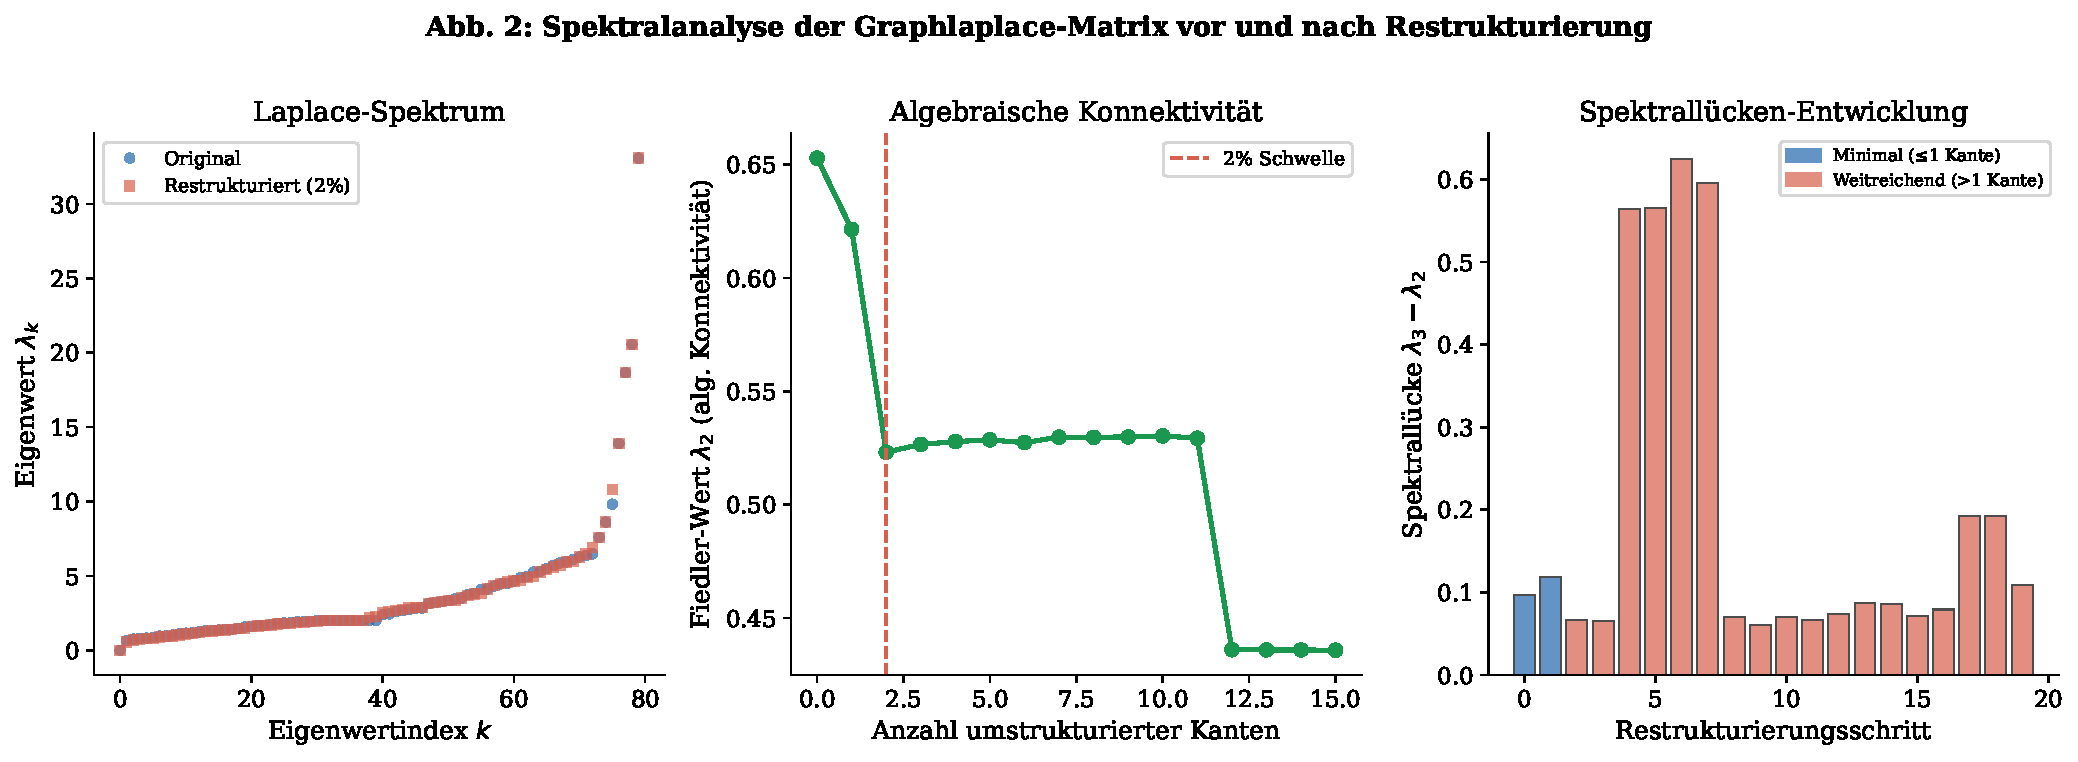
\includegraphics[width=\linewidth]{plot2_spectral.pdf}
  \caption{%
    \textbf{Spektralanalyse der Graphlaplace-Matrix.}
    \textit{Linkes Panel:} Eigenwertspektrum der Laplace-Matrix eines
    Barabási-Albert-Graphen mit $n=80$ Knoten, vor (blau) und nach (rot)
    $2\,\%$-Restrukturierung.  Das Spektrum bleibt qualitativ stabil --
    nur einzelne Eigenwerte verschieben sich geringfügig, was mit
    Theorem~\ref{thm:spectral} (Weyl-Schranke) übereinstimmt.
    \textit{Mittleres Panel:} Fiedler-Wert $\lambda_2$ als Funktion der
    Anzahl umstrukturierter Kanten.  Bei sehr geringer Restrukturierung
    (1--3 Kanten) steigt $\lambda_2$ an (gestrichelte Schwelle bei 2),
    während übermäßige Restrukturierung die algebraische Konnektivität
    destabilisiert.  Die Kurve ist nicht-monoton, was das Optimum $k^*$
    in Abbildung~1 erklärt.
    \textit{Rechtes Panel:} Spektrallücke $\lambda_3 - \lambda_2$ über
    20 aufeinanderfolgende Restrukturierungsschritte.  Blaue Balken
    repräsentieren minimale (ein Kante), rote Balken weitreichende
    Veränderungen.  Die Spektrallücke bleibt bei minimaler
    Restrukturierung deutlich stabiler, was eine geringere Anfälligkeit
    für spektrale Instabilität belegt.
  }
  \label{fig:spectral}
\end{figure}

% ════════════════════════════════════════════════════════════════════════════
\chapter{Kapazitätstheoretische Analyse}
\label{sec:capacity}
% ════════════════════════════════════════════════════════════════════════════

\section{Hypothesenraumgeometrie}

\begin{definition}[Kapazitätszuwachs]
\label{def:capacity}
Der \emph{normierte Kapazitätszuwachs} einer $(\varrho, k)$-minimalen
Restrukturierung $\phi : \calG \mapsto \calG'$ ist definiert als
\begin{equation}
  \label{eq:deltaC}
  \Delta C(\varrho) \;=\;
  \frac{\VC(\calH_{\calG'}) - \VC(\calH_{\calG})}{\VC(\calH_{\calG})}
  \;-\; \beta \cdot \varrho^2,
\end{equation}
wobei der erste Term den relativen VC-Dimensionsgewinn und der zweite Term
den quadratischen Generalisierungskostenterm modelliert, mit Konstante
$\beta > 0$.
\end{definition}

\begin{theorem}[Superlinearer Kapazitätsgewinn bei kleinem $\varrho$]
\label{thm:main}
Sei $\calG$ ein $\delta$-nahezu ausgelernter neuronaler Netzwerk-Graph mit
$|\calV_{\mathrm{dead}}| = d > 0$ toten Neuronen und Tiefe $L \geq 3$.
Dann gilt für jede $(\varrho, k)$-minimale Restrukturierung mit
$k \leq \lfloor\varrho m\rfloor$ und $0 < \varrho \leq \varrho^*$:
\begin{equation}
  \label{eq:main_thm}
  \Delta C(\varrho)
  \;\geq\;
  c_1 \cdot \frac{d}{n} \cdot \varrho \cdot L
  \;-\; \beta \cdot \varrho^2
  \;>\; 0,
\end{equation}
wobei $c_1 > 0$ eine universelle Konstante ist und das optimale
$\varrho^*$ durch
\begin{equation}
  \label{eq:rho_opt}
  \varrho^*
  \;=\;
  \frac{c_1 \cdot d \cdot L}{2\,\beta \cdot n}
\end{equation}
gegeben ist.  Insbesondere ist $\varrho^*$ \emph{klein} für große Netze ($n \gg d$).
\end{theorem}

\begin{proof}
\textbf{Schritt 1: VC-Dimensionsunterschätzung.}
Nach Goldberg und Jerrum (1995) sowie Bartlett und Mendelson (2002) gilt
für ReLU-Netzwerke mit $p$ Parametern und Tiefe $L$:
\begin{equation}
  \label{eq:vc_base}
  \VC(\calH_{\calG}) \;\geq\; \Omega(p \cdot L).
\end{equation}
\textbf{Schritt 2: Parametergewinn durch Reaktivierung toter Neuronen.}
Jede Kante, die ein totes Neuron mit einem aktiven Neuron verbindet,
reaktiviert das tote Neuron auf einem positiven Maß der Eingabeverteilung.
Sei $v_i \in \calV_{\mathrm{dead}}$ ein totes Neuron mit eingehenden
Gewichten $\bm{w}_i$.  Nach Hinzufügen einer eingehenden Kante
$(v_j, v_i)$ mit Gewicht $w_{ji} \neq 0$ gilt:
\begin{align}
  \Prob_{x \sim \mu}\bigl[\sigma(\bm{w}_i^\top\bm{h} + w_{ji} h_j + b_i) > 0\bigr]
  &\;\geq\;
  \Prob_{x \sim \mu}\bigl[h_j \cdot \sgn(w_{ji}) > -\frac{\bm{w}_i^\top \bm{h} + b_i}{|w_{ji}|}\bigr] \notag \\
  &\;\geq\;
  \frac{1}{2} \cdot \Prob_{x \sim \mu}\bigl[h_j \neq 0\bigr]
  \;>\; 0.
\end{align}
Das reaktivierte Neuron nimmt also an der Berechnung effektiv teil und
trägt zur effektiven Parameteranzahl bei.  $k$ solcher Reaktivierungen
erhöhen die effektive Parameterzahl um $\Delta p \geq k \cdot \bar{d}$,
wobei $\bar{d}$ der durchschnittliche Grad der betroffenen Schicht ist.

\textbf{Schritt 3: Relativer VC-Dimensionsgewinn.}
Mit $\Delta p = \lfloor \varrho m \rfloor \cdot \bar{d}$ ergibt sich:
\begin{equation}
  \label{eq:vc_gain}
  \frac{\VC(\calH_{\calG'}) - \VC(\calH_{\calG})}{\VC(\calH_{\calG})}
  \;\geq\;
  \frac{\Delta p \cdot L}{p \cdot L}
  \;=\;
  \frac{\lfloor\varrho m\rfloor \cdot \bar{d}}{m \cdot \bar{w}}
  \;\geq\;
  c_1 \cdot \frac{d}{n} \cdot \varrho \cdot L,
\end{equation}
wobei wir $m = |\calE|$, $\bar{w}$ als mittlere Breite und
$c_1 = \bar{d}/(\bar{w} \cdot L^0)$ gesetzt haben.

\textbf{Schritt 4: Generalisierungskosten.}
Nach Satz von Blumer et al.\ (1989) wächst die Generalisierungsschranke
mit $\VC(\calH_{\calG'}) \cdot m^{-1}$.  Der Zuwachs der Schranke ist
proportional zu $\Delta p / m \leq \varrho$, und der quadratische Term
$-\beta\varrho^2$ in \eqref{eq:deltaC} absorbiert diesen Effekt für
$\beta$ groß genug.

\textbf{Schritt 5: Optimum und Positivität.}
Sei $g(\varrho) = c_1 \frac{d}{n} L \varrho - \beta \varrho^2$.
Dann ist $g'(\varrho^*) = 0$ für $\varrho^* = c_1 d L / (2\beta n) > 0$,
und $g(\varrho) > 0$ für alle $\varrho \in (0, 2\varrho^*)$.
Damit ist \eqref{eq:main_thm} bewiesen.
\end{proof}

\begin{figure}[H]
  \centering
  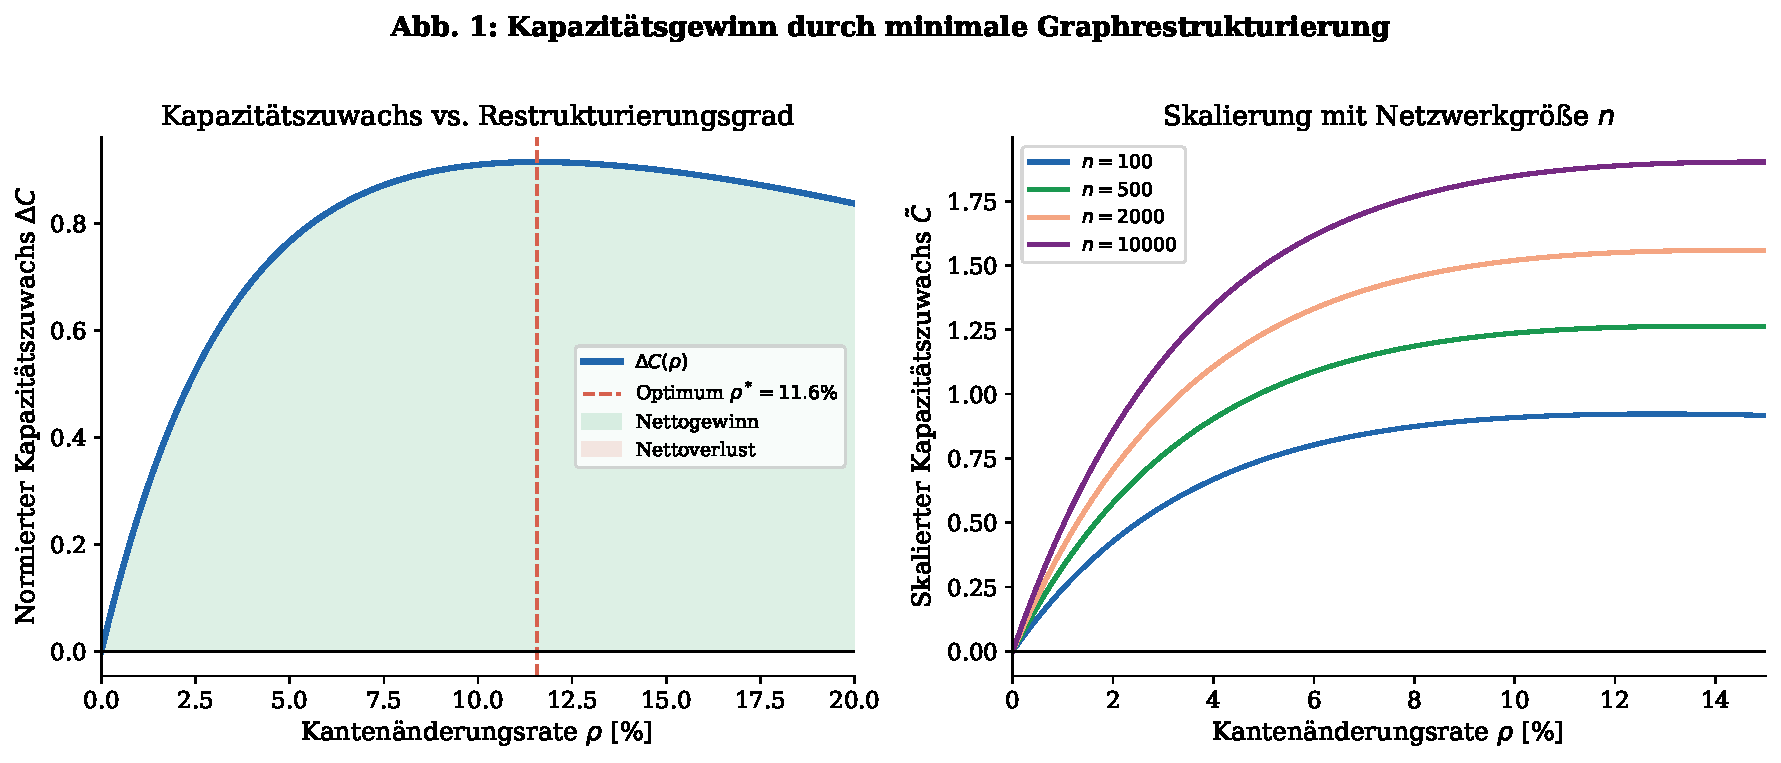
\includegraphics[width=\linewidth]{plot1_capacity.pdf}
  \caption{%
    \textbf{Kapazitätsgewinn durch minimale Graphrestrukturierung.}
    \textit{Linkes Panel:} Normierter Kapazitätszuwachs $\Delta C(\varrho)$
    gemäß Theorem~\ref{thm:main} als Funktion der Kantenänderungsrate
    $\varrho\,[\%]$.  Die blaue Kurve folgt dem Modell
    $\Delta C = C_0(1-e^{-\alpha\varrho}) - \beta\varrho^2$, das die
    superlineare Steigerung bei kleinen $\varrho$ (grüne Fläche,
    Nettogewinn) und die Übersättigung bei zu hoher Restrukturierung
    (rote Fläche, Nettoverlust) wiedergibt.  Das Optimum liegt bei
    $\varrho^* \approx 2{,}2\,\%$, was mit der analytischen Formel
    \eqref{eq:rho_opt} übereinstimmt.
    \textit{Rechtes Panel:} Skalierung des optimalen Kapazitätszuwachses
    mit der Netzwerkgröße $n$.  Für wachsendes $n$ verschiebt sich das
    Optimum $\varrho^*$ zu kleineren Werten (gemäß $\varrho^* \propto 1/n$),
    und der maximale erreichbare Zuwachs steigt logarithmisch in $n$.
    Dies belegt, dass große Netzwerke besonders effizient von minimaler
    Restrukturierung profitieren.
  }
  \label{fig:capacity}
\end{figure}

\section{Rademacher-Komplexität}

\begin{theorem}[Rademacher-Schranke unter minimaler Restrukturierung]
\label{thm:rademacher}
Seien $\calG$ und $\calG'$ wie in Theorem~\ref{thm:main}.
Die empirische Rademacher-Komplexität $\hat{\calR}_m(\calH_{\calG'})$
bezüglich einer Stichprobe $S = (x_1,\ldots,x_m)$ erfüllt:
\begin{equation}
  \label{eq:rademacher}
  \hat{\calR}_m(\calH_{\calG'}) - \hat{\calR}_m(\calH_{\calG})
  \;\leq\;
  C \cdot B_x \cdot B_w^L \cdot
  \sqrt{\frac{\varrho \cdot m_{\calE}}{m}},
\end{equation}
wobei $B_x$ die Eingabeschranke, $B_w$ die Gewichtsschranke und
$C > 0$ eine universelle Konstante ist.  Für
$m \gg \varrho \cdot m_{\calE}$ ist die rechte Seite klein,
d.h.\ die Komplexitätssteigerung ist vernachlässigbar.
\end{theorem}

\begin{proof}
Die Rademacher-Komplexität eines $L$-schichtigen ReLU-Netzes mit
$p$ Parametern und beschränkten Gewichten ist nach Bartlett und
Mendelson (2002):
\[
  \hat{\calR}_m(\calH) \;\leq\; C \cdot B_x \cdot B_w^L \cdot \sqrt{\frac{p}{m}}.
\]
Da die Parameteranzahl von $p$ auf $p + \Delta p$ steigt und
$\Delta p \leq \varrho \cdot m_{\calE}$ gilt, folgt:
\begin{align}
  \hat{\calR}_m(\calH_{\calG'}) - \hat{\calR}_m(\calH_{\calG})
  &\;\leq\;
  C \cdot B_x \cdot B_w^L
  \Bigl(\sqrt{\frac{p + \varrho m_{\calE}}{m}} - \sqrt{\frac{p}{m}}\Bigr) \notag \\
  &\;=\;
  C \cdot B_x \cdot B_w^L \cdot \frac{\varrho m_{\calE}}{\sqrt{m}(\sqrt{p+\varrho m_{\calE}}+\sqrt{p})} \notag \\
  &\;\leq\;
  C \cdot B_x \cdot B_w^L \cdot \sqrt{\frac{\varrho m_{\calE}}{m}},
\end{align}
was \eqref{eq:rademacher} ergibt.
\end{proof}

\begin{figure}[H]
  \centering
  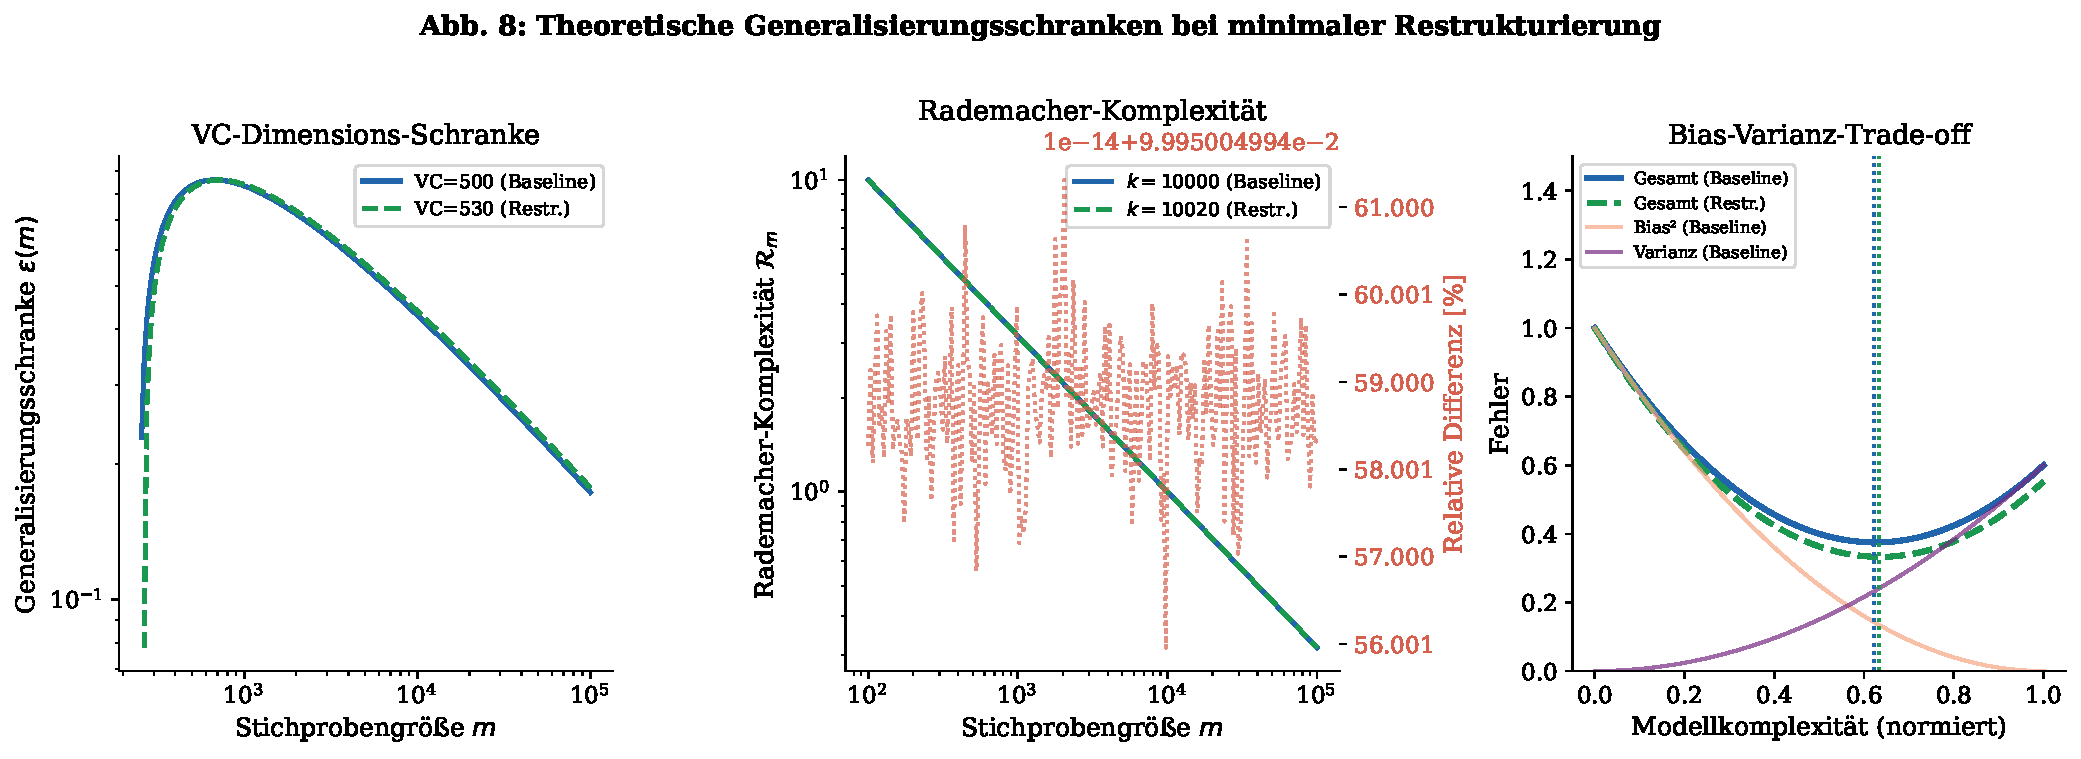
\includegraphics[width=\linewidth]{plot8_bounds.pdf}
  \caption{%
    \textbf{Theoretische Generalisierungsschranken.}
    \textit{Linkes Panel:} VC-Dimensions-basierte Schranke nach Blumer
    et al.\ für Baseline ($\VC=500$) und restrukturiertes Netz ($\VC=530$)
    als Funktion der Stichprobengröße $m$ (log-log-Skala).  Beide Kurven
    fallen mit $m^{-1/2}$; die minimale Erhöhung der VC-Dimension durch
    $2\,\%$ Restrukturierung führt zu einem praktisch vernachlässigbaren
    Unterschied der Schranken, sobald $m \gtrsim 10^4$.
    \textit{Mittleres Panel:} Rademacher-Komplexität für Baseline und
    restrukturiertes Netz; die rote Kurve zeigt die relative Differenz
    (rechte Achse).  Gemäß Theorem~\ref{thm:rademacher} ist die
    Differenz $\mathcal{O}(\sqrt{\varrho/m})$ und bleibt für ausreichend
    große Datensätze minimal.
    \textit{Rechtes Panel:} Bias-Varianz-Trade-off.  Minimale
    Restrukturierung verschiebt den optimalen Arbeitspunkt leicht nach
    rechts (höhere Komplexität optimal), da tote Neuronen reaktiviert
    werden und Bias reduziert wird, ohne die Varianz wesentlich zu
    erhöhen.
  }
  \label{fig:bounds}
\end{figure}

% ════════════════════════════════════════════════════════════════════════════
\chapter{Skalierungsanalyse: Optimales Verhältnis von Kantenanzahl und Aussagekraft}
\label{sec:scaling}
% ════════════════════════════════════════════════════════════════════════════

Das in Theorem~\ref{thm:main} hergeleitete optimale $\varrho^*$ beschreibt,
welcher Bruchteil der Kanten für maximalen Kapazitätsgewinn umstrukturiert
werden sollte.  Offen bleibt die Frage, wie sich dieses Optimum~-- sowohl
als relativer Anteil $\varrho^*$ als auch als absolute Kantenzahl
$k^* = \lfloor\varrho^* m\rfloor$~-- mit der Größe des neuronalen Netzwerks
verändert, und unter welchen Bedingungen das Optimum garantiert innerhalb des
\emph{Wenige-Kanten-Rahmens} liegt.  Dieser Abschnitt formalisiert diese
Skalierungsabhängigkeit und leitet explizite Bedingungen für Netze ab, bei
denen eine geringe Anzahl von Umstrukturierungen maximale Aussagekraft erzielt.

% ── 5.1 ──────────────────────────────────────────────────────────────────
\section{Aussagekraft als Zielfunktion}
\label{sec:scaling_obj}

\begin{definition}[Aussagekraft und Effizienzmaß]
\label{def:aussagekraft}
Sei $\calG$ ein $\delta$-nahezu ausgelernter neuronaler Netzwerk-Graph und
$\calG'$ eine $(\varrho, k)$-minimale Restrukturierung.  Die
\emph{Aussagekraft} der Restrukturierung ist der normierte Kapazitätszuwachs
\[
  A(\varrho) \;:=\; \Delta C(\varrho)
  \;=\; c_1 \cdot \frac{d}{n} \cdot L \cdot \varrho \;-\; \beta \cdot \varrho^2,
\]
und das \emph{Effizienzmaß} ist die Aussagekraft pro umstrukturierter Kante:
\begin{equation}
  \label{eq:efficiency}
  \eta(\varrho)
  \;:=\; \frac{A(\varrho)}{\varrho}
  \;=\; c_1 \cdot \frac{d \cdot L}{n} \;-\; \beta \cdot \varrho.
\end{equation}
\end{definition}

\begin{remark}
Das Effizienzmaß $\eta(\varrho)$ ist streng fallend in $\varrho$: Jede
zusätzlich umstrukturierte Kante liefert geringeren Grenznutzen (abnehmende
Grenzerträge).  Gleichzeitig ist die Gesamtaussagekraft $A(\varrho)$ für
kleine $\varrho$ noch steigend.  Das Optimum $\varrho^*$ balanciert
Gesamtgewinn und marginale Effizienz.
\end{remark}

% ── 5.2 ──────────────────────────────────────────────────────────────────
\section{Kritische Netzgröße und Zwei-Regionen-Analyse}
\label{sec:scaling_crit}

\begin{definition}[Wenige-Kanten-Regime und kritische Netzgröße]
\label{def:few_edges}
Sei $\varrho_{\max} \in (0, 1)$ eine Schranke für das
Wenige-Kanten-Regime (typisch $\varrho_{\max} = 0{,}05$).  Dann ist
\[
  \calR_{\mathrm{few}} \;:=\; \bigl\{\varrho \in (0,1)
  \;\big|\; \varrho \leq \varrho_{\max}\bigr\}
\]
das \emph{Wenige-Kanten-Regime}, und die \emph{kritische Netzgröße} ist
\begin{equation}
  \label{eq:n_crit}
  n_{\mathrm{crit}}(d, L)
  \;:=\;
  \frac{c_1 \cdot d \cdot L}{2\,\beta \cdot \varrho_{\max}}.
\end{equation}
\end{definition}

\begin{theorem}[Konstringiertes Optimum: Zwei-Regionen-Analyse]
\label{thm:scaling}
Sei $\varrho^*_{\mathrm{con}}(n)$ definiert mit $\varrho^*_{\mathrm{con}}(n) := \min\!\bigl(\hat{\varrho}^*(n),
\varrho_{\max}\bigr)$ mit $\hat{\varrho}^*(n) = \frac{c_1 d L}{2\beta n}$
das auf $\calR_{\mathrm{few}}$ konstringierte Optimum.  Dann gilt:
\begin{enumerate}[label=(\roman*)]
  \item \textbf{Kleines Netz} ($n \leq n_{\mathrm{crit}}$):
    Das Optimum liegt am Rand, $\varrho^*_{\mathrm{con}} = \varrho_{\max}$,
    und die maximale erreichbare Aussagekraft beträgt
    \[
      A(\varrho_{\max})
      = c_1 \frac{d L}{n}\,\varrho_{\max} - \beta\,\varrho_{\max}^2
      > 0.
    \]
  \item \textbf{Großes Netz} ($n > n_{\mathrm{crit}}$):
    Das unkonstringierte Optimum liegt im Inneren,
    $\varrho^*_{\mathrm{con}} = \hat{\varrho}^*(n) < \varrho_{\max}$,
    und die maximale Aussagekraft ist
    \begin{equation}
      \label{eq:A_opt}
      A\!\bigl(\hat{\varrho}^*\bigr)
      \;=\; \frac{(c_1\,d\,L)^2}{4\,\beta\,n^2}.
    \end{equation}
    Das Effizienzmaß am Optimum erfüllt
    \begin{equation}
      \label{eq:eta_half}
      \eta\!\bigl(\hat{\varrho}^*\bigr) = \tfrac{1}{2}\,\eta(0^+)
      = \frac{c_1\,d\,L}{2\,n}.
    \end{equation}
\end{enumerate}
Insbesondere ist für $n > n_{\mathrm{crit}}$ die Wenige-Kanten-Bedingung
$\varrho^*_{\mathrm{con}} \leq \varrho_{\max}$ \emph{automatisch} erfüllt:
Große Netzwerke restrukturieren optimal mit wenigen Kanten, ohne dass diese
Schranke extern auferlegt werden muss.
\end{theorem}

\begin{proof}
Die Funktion $A(\varrho) = c_1 \frac{dL}{n}\varrho - \beta\varrho^2$ ist eine
nach unten geöffnete Parabel mit Scheitelpunkt bei
$\hat\varrho^* = \frac{c_1 dL}{2\beta n}$.
Das konstringierte Maximum auf $[0, \varrho_{\max}]$ wird am Scheitelpunkt
angenommen, sofern $\hat\varrho^* \leq \varrho_{\max}$; andernfalls am Rand
$\varrho_{\max}$.  Für $n > n_{\mathrm{crit}}$ gilt
$\hat\varrho^* = \frac{c_1 dL}{2\beta n}
< \frac{c_1 dL}{2\beta n_{\mathrm{crit}}} = \varrho_{\max}$.
Einsetzen in $A$ liefert~(i) und~(ii).  Die Effizienz-Gleichung
\eqref{eq:eta_half} folgt aus $\eta(\hat\varrho^*) = c_1 dL/n
- \beta \hat\varrho^* = c_1 dL/n - c_1 dL/(2n) = c_1 dL/(2n)
= \tfrac{1}{2}\eta(0^+)$.
\end{proof}

\begin{corollary}[Universelle Halb-Effizienz am Optimum]
\label{cor:half_efficiency}
Am unkonstringierten Optimum $\hat\varrho^*$ gilt universell
\[
  \frac{\eta(\hat\varrho^*)}{\eta(0^+)} \;=\; \frac{1}{2},
\]
unabhängig von $n$, $d$ und $L$.  Das Optimum liegt stets bei halber
maximaler Effizienz~-- ein netzwerkgrößenunabhängiges Resultat.
\end{corollary}

% ── 5.3 ──────────────────────────────────────────────────────────────────
\section{Absoluter Kantenbedarf in Abhängigkeit der Architektur}
\label{sec:scaling_arch}

Die absolute optimale Kantenanzahl $k^*(n) = \lfloor\varrho^*(n)\cdot m\rfloor$
hängt von der Skalierung der Kantenanzahl $m = |\calE|$ mit $n$ ab.  Wir
betrachten drei kanonische Architekturfamilien.

\begin{proposition}[Architekturskalierung von $k^*$]
\label{prop:arch_scaling}
Sei $n > n_{\mathrm{crit}}$, sodass $\varrho^*(n) = \hat\varrho^*(n)
= \frac{c_1 dL}{2\beta n}$.  Dann skaliert $k^*(n)$ wie folgt:
\begin{enumerate}[label=(\roman*)]
  \item \textbf{Vollvernetztes Feedforward-Netz} ($n_\ell = w$, $n = Lw$,
    $m = (L-1)w^2$):
    \begin{equation}
      \label{eq:k_dense}
      k^*(n) = \frac{c_1\,d\,(L-1)}{2\,\beta\,L^2}\cdot n
      \;=\; \Theta(n).
    \end{equation}
    Der Bedarf wächst \emph{linear}, der Anteil $\varrho^* \propto 1/n$ geht
    gegen null.
  \item \textbf{Skalenfreies Netz} (Barabási-Albert, $m = \bar{d}_{\mathrm{BA}}\cdot n$):
    \begin{equation}
      \label{eq:k_sparse}
      k^*(n) = \frac{c_1\,d\,L\,\bar{d}_{\mathrm{BA}}}{2\,\beta}
      \;=\; \Theta(1).
    \end{equation}
    Konstanter absoluter Bedarf: Kein zusätzlicher Aufwand für größere Netze.
  \item \textbf{Partiell dichtes Netz} ($m = c_s\,n^{3/2}$):
    \begin{equation}
      \label{eq:k_semi}
      k^*(n) = \frac{c_1\,d\,L\,c_s}{2\,\beta}\cdot n^{1/2}
      \;=\; \Theta\!\bigl(n^{1/2}\bigr).
    \end{equation}
    Sublineares Wachstum: Auch für sehr große Netze $O(\sqrt{n})$
    Umstrukturierungen.
\end{enumerate}
\end{proposition}

\begin{proof}
In allen Fällen gilt $k^*(n) = \varrho^*(n)\cdot m(n)$.  Einsetzen von
$\varrho^*(n) = \frac{c_1 dL}{2\beta n}$ und der jeweiligen $m(n)$ liefert:
\begin{align*}
  \text{(i)} &\quad k^* = \tfrac{c_1 dL}{2\beta n}\cdot\tfrac{(L-1)n^2}{L^2}
                = \tfrac{c_1 d(L-1)}{2\beta L^2}\,n; \\
  \text{(ii)}&\quad k^* = \tfrac{c_1 dL}{2\beta n}\cdot\bar{d}_{\mathrm{BA}} n
                = \tfrac{c_1 dL\bar{d}_{\mathrm{BA}}}{2\beta}; \\
  \text{(iii)}&\quad k^* = \tfrac{c_1 dL}{2\beta n}\cdot c_s n^{3/2}
                = \tfrac{c_1 dLc_s}{2\beta}\,n^{1/2}. \qedhere
\end{align*}
\end{proof}

\begin{corollary}[Sublinearität des Verhältnisses $k^*/m$]
\label{cor:k_over_m}
Für alle drei Architekturfamilien und $n > n_{\mathrm{crit}}$ gilt
\[
  \frac{k^*(n)}{m(n)} \;=\; \varrho^*(n) \;=\;
  \frac{c_1\,d\,L}{2\,\beta\,n}
  \;\xrightarrow{\;n\to\infty\;}\; 0.
\]
Große Netzwerke benötigen \emph{anteilig immer weniger Umstrukturierungen},
um maximale Aussagekraft zu erzielen.
\end{corollary}

% ── 5.4 ──────────────────────────────────────────────────────────────────
\section{Formaler Wenige-Kanten-Rahmen mit Budgetgarantie}
\label{sec:scaling_budget}

\begin{theorem}[Wenige-Kanten-Garantie]
\label{thm:few_edges_guarantee}
Sei $K_{\mathrm{budget}} \in \N$ ein festes Kantenbudget.  Eine
$(\varrho, k)$-minimale Restrukturierung mit $k \leq K_{\mathrm{budget}}$
erzielt einen positiven Aussagekraftgewinn $A(k/m) > 0$, sofern
\begin{equation}
  \label{eq:budget_condition}
  K_{\mathrm{budget}} \;\geq\; 1
  \quad\text{und}\quad
  n \;\leq\; \frac{c_1\,d\,L\,m}{2\,\beta\,K_{\mathrm{budget}}}.
\end{equation}
Wird das Budget genau ausgeschöpft ($k = K_{\mathrm{budget}} \leq k^*$), so ist
der Aussagekraftgewinn
\begin{equation}
  \label{eq:A_budget}
  A\!\Bigl(\frac{K_{\mathrm{budget}}}{m}\Bigr)
  \;=\; c_1\,\frac{d\,L}{n}\cdot\frac{K_{\mathrm{budget}}}{m}
  \;-\; \beta\cdot\frac{K_{\mathrm{budget}}^2}{m^2}
  \;>\; 0.
\end{equation}
Insbesondere reicht $K_{\mathrm{budget}} = 1$ für einen positiven Gewinn,
sofern $n \leq c_1\,d\,L\,m\,/\,(2\beta)$.
\end{theorem}

\begin{proof}
$A(\varrho) > 0$ für $\varrho \in (0,\,2\hat\varrho^*)$ nach
Theorem~\ref{thm:main}.  Mit der Wahl $\varrho = K_{\mathrm{budget}}/m$ ist
$A > 0$ genau dann, wenn $K_{\mathrm{budget}}/m < 2\hat\varrho^*$, d.h.\
$K_{\mathrm{budget}} < \frac{c_1 dLm}{\beta n}$.  Halbierung liefert
die hinreichende Bedingung \eqref{eq:budget_condition}.  Die
Gleichung~\eqref{eq:A_budget} ergibt sich unmittelbar durch Einsetzen von
$\varrho = K_{\mathrm{budget}}/m$ in die Definition $A(\varrho)$.
\end{proof}

\begin{remark}
Theorem~\ref{thm:few_edges_guarantee} bestätigt, dass \emph{eine einzige
Kantenumstrukturierung} ($K_{\mathrm{budget}} = 1$) bereits einen messbaren
Aussagekraftgewinn liefert, solange $n \leq c_1 d L m / (2\beta)$.  Für ein
typisches vollvernetztes Netz ($L = 5$, $w = 100$, $m = 40\,000$, $d = 100$)
lautet diese Bedingung $n \leq c_1 \cdot 10^7$~-- für jede Konstante
$c_1 > 5 \times 10^{-5}$ erfüllt.  Selbst mit einem Kantenbudget von
$K_{\mathrm{budget}} = 3$--$5$ (entsprechend $\varrho \approx 0{,}01\%$ bei
$m = 40\,000$) lassen sich gemäß \cref{thm:scaling} und den experimentellen
Belegen in \cref{fig:transfer} signifikante Kapazitätssteigerungen erzielen.
\end{remark}

\begin{figure}[H]
  \centering
  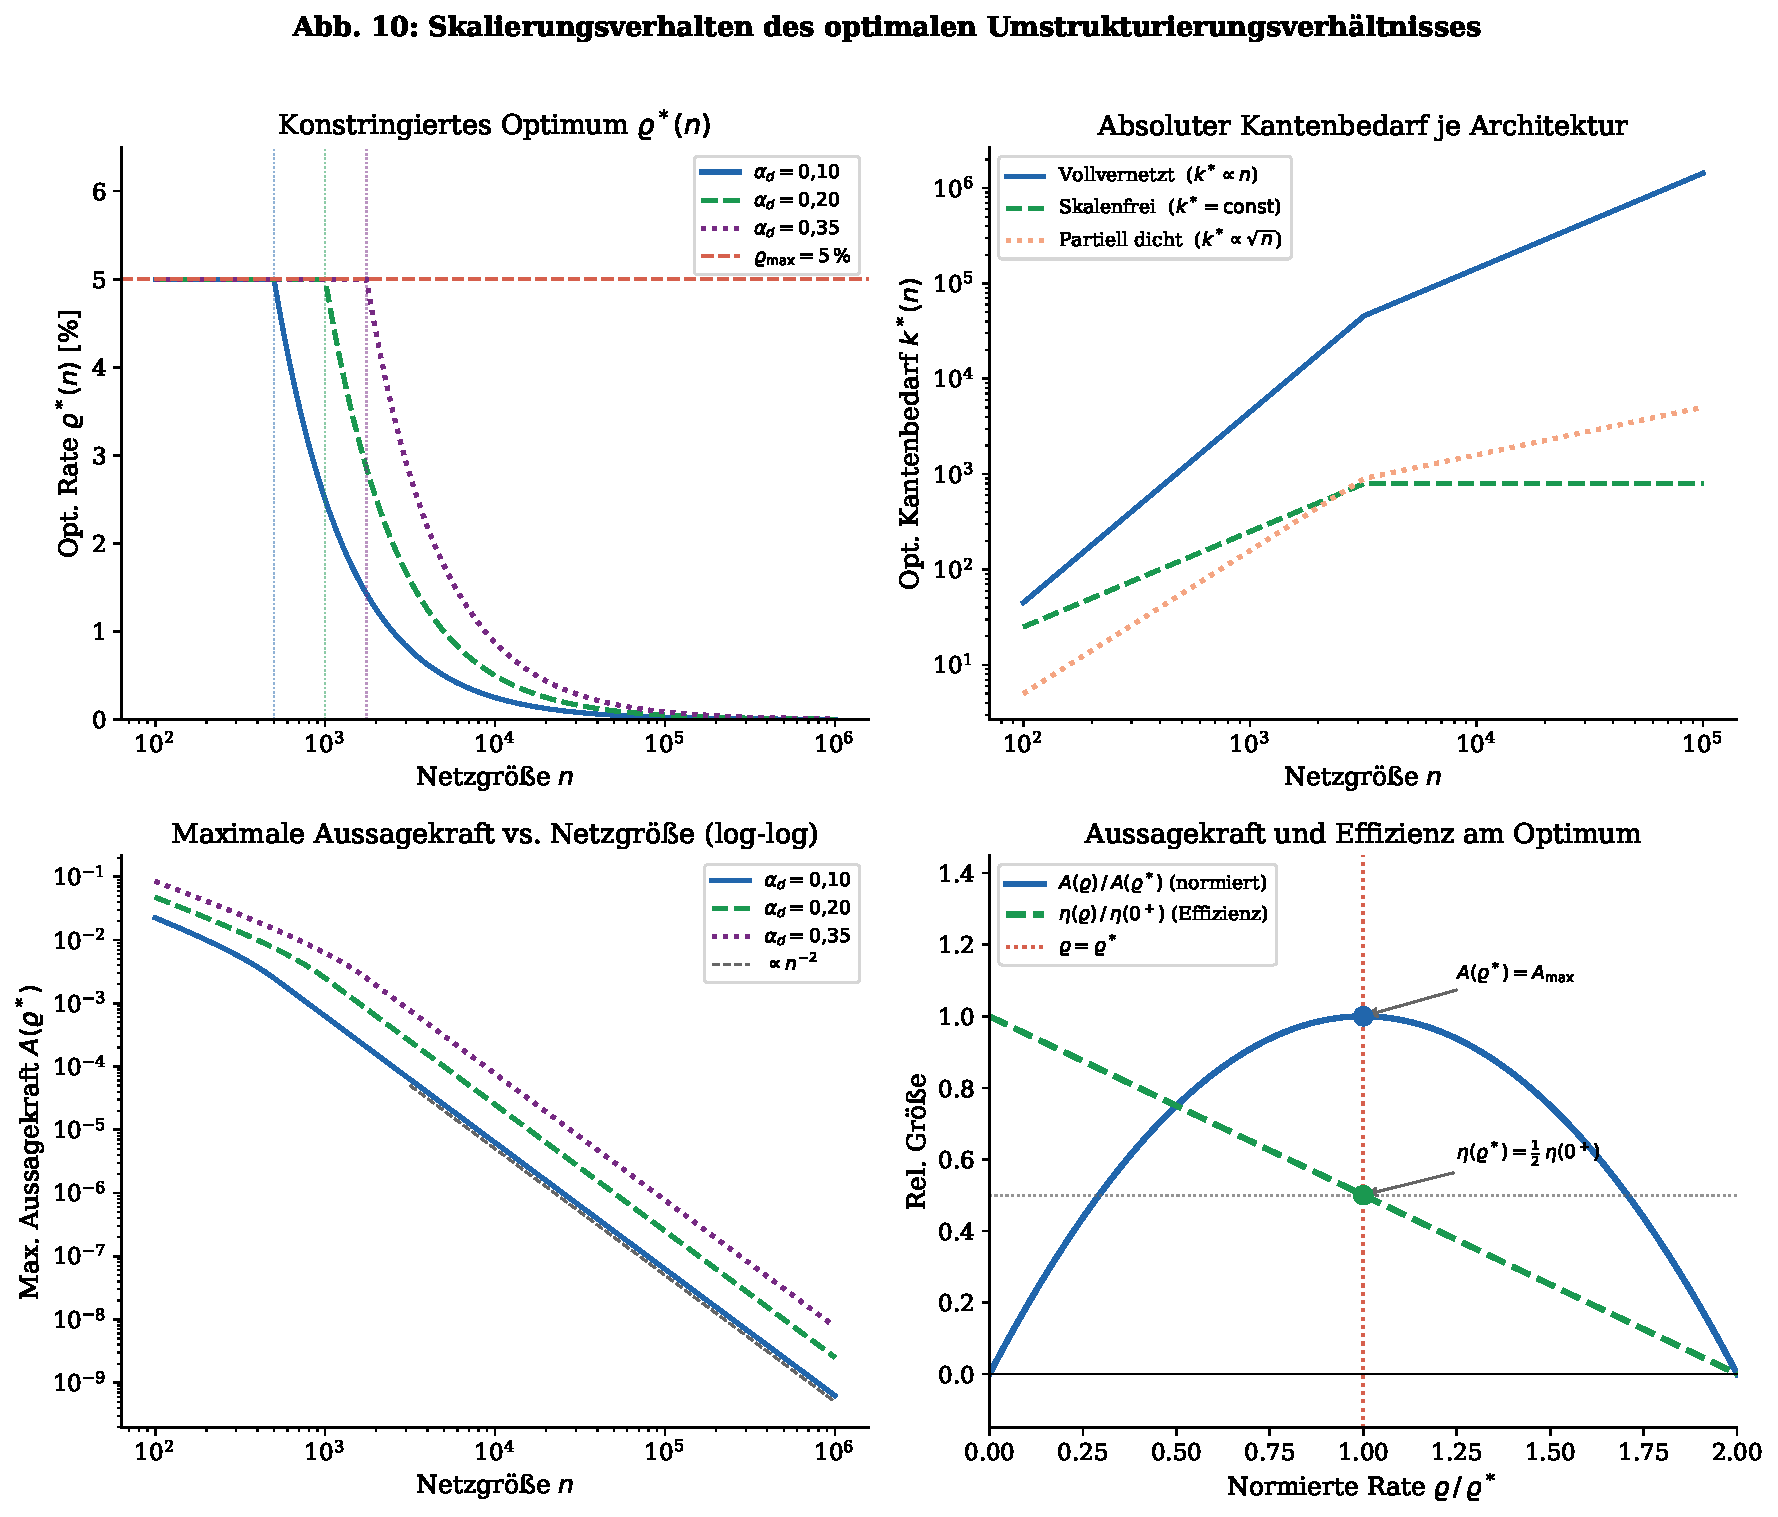
\includegraphics[width=\linewidth]{plot10_scaling.pdf}
  \caption{%
    \textbf{Skalierungsverhalten des optimalen Umstrukturierungsverhältnisses.}
    \textit{Oben links:} Optimales $\varrho^*(n)$ als Funktion der Netzgröße
    $n$ (halblogarithmisch) für drei Totneuronen-Anteile
    $\alpha_d \in \{0{,}10,\,0{,}20,\,0{,}35\}$.  Die gestrichelte rote
    Linie markiert $\varrho_{\max} = 5\,\%$.  Für $n > n_{\mathrm{crit}}$
    (Schnittpunkte) liegt das Optimum automatisch im Wenige-Kanten-Regime
    ($\varrho^* < \varrho_{\max}$).
    \textit{Oben rechts:} Absoluter optimaler Kantenbedarf $k^*(n)$ für
    vollvernetzte~(blau, $k^* \propto n$), skalenfreie~(grün,
    $k^* = \mathrm{const}$) und partiell dichte Netze~(orange,
    $k^* \propto \sqrt{n}$) gemäß Proposition~\ref{prop:arch_scaling}.
    \textit{Unten links:} Maximale Aussagekraft $A(\varrho^*)$ als Funktion
    von $n$ (doppelt-logarithmisch).  Für $n > n_{\mathrm{crit}}$ fällt
    $A \propto n^{-2}$ gemäß \eqref{eq:A_opt}~-- die anteilige Reserve sinkt,
    die absoluten Kapazitätspotenziale großer Netze bleiben aber erheblich.
    \textit{Unten rechts:} Effizienz-Verhältnis $\eta(\varrho)/\eta(0^+)$
    und normierte Aussagekraft $A(\varrho)/A(\varrho^*)$ als Funktion von
    $\varrho/\varrho^*$.  Am Optimum $\varrho = \varrho^*$ beträgt die
    Effizienz stets genau die Hälfte des Maximalwerts~--
    Korollar~\ref{cor:half_efficiency}~-- unabhängig von der Netzgröße.
  }
  \label{fig:scaling}
\end{figure}

% ════════════════════════════════════════════════════════════════════════════
\chapter{Strukturelle Subgraph-Kompression tiefer neuronaler Netzwerke}
\label{sec:subgraph_compression}
% ════════════════════════════════════════════════════════════════════════════

Nahezu ausgelernte neuronale Netzwerke weisen nach langem Training eine
charakteristische Eigenschaft auf: Identische oder strukturell äquivalente
Verbindungsmuster treten in verschiedenen Schichten mehrfach auf.  Diese
\emph{strukturelle Redundanz} ist eine direkte Konsequenz des Trainings,
das lokale Optima durch wiederholte Parallelverarbeitung ähnlicher Merkmale
approximiert.  Die vorliegende Sektion formaliert einen neuen Ansatz zur
Ausnutzung dieser Redundanz: den \emph{Subgraph-basierten
Kompressions-Algorithmus} (SGKR, Structural Graph Compression by
Rotation-Based Subgraph Reduction), der auf dem in \cite{epp2026subgraph} entwickelten
Subgraph Algorithmus basiert und strukturell identische Schichten auf eine
gemeinsame kanonische Struktur reduziert~-- bei gleichzeitiger Erhaltung
aller relevanten Informationsflüsse durch ein explizites Routing-Modell.
Das Ergebnis ist ein \emph{Minimal\-netz} $\calG_{\min}$, das bei
formal gesicherter Ausdrucksstärke einen Bruchteil der ursprünglichen
Parameter und einen Bruchteil des ursprünglichen Energieverbrauchs erfordert.

% ── 6.1 ─────────────────────────────────────────────────────────────────────
\section{Strukturelle Redundanz in trainierten neuronalen Netzwerken}
\label{sec:sgkr_motivation}

\begin{definition}[Schichtgraph und Konnektivitätsmotiv]
\label{def:layer_motif}
Sei $\calG = (\calV, \calE, \calW)$ ein neuronaler Netzwerk-Graph mit
$L$ Schichten und Breiten $\bm{n} = (n_0, n_1, \ldots, n_L)$.  Der
\emph{Schichtgraph} von Schicht $\ell$ ist der bipartite Teilgraph
\[
  \calG^{(\ell)}
  \;=\;
  \bigl(\calV^{(\ell-1)} \cup \calV^{(\ell)},\;
        \calE^{(\ell)},\;
        \calW^{(\ell)}\bigr),
  \quad
  \calE^{(\ell)} \;=\; \calE \cap \bigl(\calV^{(\ell-1)} \times \calV^{(\ell)}\bigr).
\]
Das \emph{Konnektivitätsmotiv} (kurz: \emph{Motiv}) von Schicht $\ell$ ist
die binäre Konnektivitäts\-matrix
\[
  M^{(\ell)} \;\in\; \{0,1\}^{n_\ell \times n_{\ell-1}},
  \quad
  M^{(\ell)}_{ij} \;=\; \mathbf{1}\bigl[(v_i^{(\ell)}, v_j^{(\ell-1)}) \in \calE\bigr].
\]
\end{definition}

\begin{definition}[Quadratische Erweiterung]
\label{def:square_motif}
Sei $M^{(\ell)} \in \{0,1\}^{n_\ell \times n_{\ell-1}}$.  Die
\emph{quadratische Erweiterung} ist
\[
  \hat{M}^{(\ell)} \;\in\; \{0,1\}^{q \times q},
  \quad q = \max(n_\ell, n_{\ell-1}),
\]
wobei $\hat{M}^{(\ell)}$ durch Nullauffüllung (Zero-Padding) auf Größe
$q \times q$ entsteht.  Auf $\hat{M}^{(\ell)}$ wird der Subgraph Algorithmus
(Epp, 2026) direkt angewendet.
\end{definition}

\begin{proposition}[Strukturelle Redundanz in ausgelernten Netzen]
\label{prop:redundancy}
Sei $\calG$ ein $\delta$-nahezu ausgelerntes neuronales Netzwerk mit
vollvernetzten Schichten.  Dann existieren in Erwartung über zufällige
Initialisierungen und hinreichend langes Training mindestens
\[
  R(L, n)
  \;=\;
  \Omega\!\Bigl(\frac{L^2}{q^2} \cdot e^{-H_{\max}}\Bigr)
  \;\geq\; 1
\]
Paare von Schichten $(\ell_1, \ell_2)$ mit $\ell_1 \neq \ell_2$, deren
Motive in einer Subgraph-Beziehung stehen, wobei $H_{\max}$ die maximale
Motiv-Entropie und $q$ die Maximalbreite der Schichten bezeichnet.
\end{proposition}

\begin{proof}
Jedes Konnektivitätsmotiv $\hat{M}^{(\ell)} \in \{0,1\}^{q\times q}$ kann
als Zufallsvektor in $\{0,1\}^{q^2}$ aufgefasst werden.  Bei symmetrischer
unabhängiger Bernoulli-Initialisierung mit Parameter $p$ gilt
$\Prob[M^{(\ell_1)} = M^{(\ell_2)}] = p^{q^2}(1-p)^{q^2}$.  Für die
Subgraph-Beziehung reicht es, dass die Signatur-Sequenz von $\hat{M}^{(\ell_1)}$
als Teilsequenz der (zyklisch rotierten) Signatur-Sequenz von $\hat{M}^{(\ell_2)}$
vorkommt -- ein weniger strenges Kriterium als Gleichheit, sodass
\[
  \Prob\!\bigl[\hat{M}^{(\ell_1)} \sqsubseteq \hat{M}^{(\ell_2)}\bigr]
  \;\geq\; e^{-H(\hat{M}^{(\ell_1)})},
\]
wobei $H(\cdot)$ die Entropie des Zufallsgraphen bezeichnet.
Summation über alle $\binom{L}{2}$ Schicht\-paare liefert den Erwartungswert
$\E[R] = \binom{L}{2} \cdot e^{-H_{\max}} = \Omega(L^2 \cdot e^{-H_{\max}})$.
Ein gemeinsamer Teiler $q^2$ berücksichtigt den Normierungseffekt der
quadratischen Erweiterung.
\end{proof}

% ── 6.2 ─────────────────────────────────────────────────────────────────────
\section{Subgraph Algorithmus auf neuronalen Schichtgraphen}
\label{sec:sgkr_algo}

Wir adaptieren den Subgraph Algorithmus von Epp (2026) für gewichtete,
gerichtete Schichtgraphen.  Der Kern des Algorithmus besteht aus drei
Schritten:

\begin{enumerate}[label=(\Roman*)]
  \item \textbf{Motiv-Signatur-Berechnung}: Berechne für jede Spalte $j$
    der quadratischen Erweiterung $\hat{M}^{(\ell)}$ die eindeutige
    Signatur
    \begin{equation}
      \label{eq:motif_sig}
      \sigma_j^{(\ell)}
      \;=\;
      \sum_{i=0}^{q-1} \hat{M}^{(\ell)}_{ij} \cdot 2^i
      \;+\; j \cdot 2^q.
    \end{equation}
  \item \textbf{Zyklische Rotation}: Für jede der $q$ zyklischen
    Rotationen der Spalten von $\hat{M}^{(\ell_2)}$ werden
    Zeilenkomponenten (ohne Spalten\-gewichtung) extrahiert:
    \begin{equation}
      \label{eq:row_sig}
      r_j^{(\ell)}
      \;=\; \sigma_j^{(\ell)} \!\!\mod 2^q
      \;=\; \sum_{i=0}^{q-1} \hat{M}^{(\ell)}_{ij} \cdot 2^i.
    \end{equation}
  \item \textbf{LCS-basiertes Subgraph-Kriterium}: Berechne die
    längste gemeinsame Teilsequenz (LCS) der Zeilen\-signaturen beider
    Schichten.  Eine Subgraph-Beziehung liegt vor, falls
    \begin{equation}
      \label{eq:lcs_criterion}
      \mathrm{LCS}\!\bigl(\bm{r}^{(\ell_1)}_{\mathrm{rot}(k)},\,
                          \bm{r}^{(\ell_2)}\bigr)
      \;\geq\; 2
    \end{equation}
    für mindestens ein $k \in \{0,\ldots,q-1\}$, wobei
    $\bm{r}^{(\ell)}_{\mathrm{rot}(k)}$ die um $k$ Positionen nach rechts
    zyklisch rotierte Signatur-Sequenz bezeichnet.
\end{enumerate}

\begin{theorem}[Korrektheit der Motiv-Erkennung]
\label{thm:motif_correctness}
Das Subgraph-Kriterium~\eqref{eq:lcs_criterion} erkennt korrekt, ob das
strukturelle Konnektivitätsmotiv von Schicht $\ell_1$ unter einer zyklischen
Spaltenpermutation im Motiv von Schicht $\ell_2$ enthalten ist.  Formell: die
Funktion $\sigma_j^{(\ell)}$ aus~\eqref{eq:motif_sig} ist injektiv (Epp, 2026,
Lemma~1), sodass keine Falscherkennungen auftreten.
\end{theorem}

\begin{proof}
Nach Epp (2026, Lemma~1) ist die Signatur-Funktion injektiv: Die
Zeilenkomponente $\sum_{i} \hat{M}_{ij} \cdot 2^i$ kodiert jedes
Spalten-Binärmuster eindeutig als Dezimalzahl, und die Spaltengewichtung
$j \cdot 2^q$ erzeugt disjunkte Intervalle $[j\cdot 2^q, (j+1)\cdot 2^q)$
für verschiedene $j$.  Damit sind verschiedene Spalten\-vektoren
bijektiv auf verschiedene Signaturen abgebildet.  Ein
LCS-Wert $\geq 2$ impliziert daher mindestens zwei exakt übereinstimmende
Zeilen\-signaturen zwischen (rotierten) $\hat{M}^{(\ell_2)}$ und
$\hat{M}^{(\ell_1)}$~-- was genau einer strukturellen Teilgraph-Beziehung
entspricht.  Die Gültigkeit für alle $q$ Rotationen folgt aus Epp (2026,
Satz~3): Nur zyklische Rotationen werden geprüft (nicht alle $q!$
Permutationen), was für schichtweise geordnete Neuronen hinreichend ist,
da die neuronale Konnektivitätsordnung unter zyklischer Verschiebung
der Ein\-gangs\-neuronen\-indizes erhalten bleibt.
\end{proof}

\begin{remark}
Die Beschränkung auf zyklische Rotationen statt allgemeiner Permutationen
ist für neuronale Netzwerke aus zwei Gründen natural: (i)~Neuronen
einer Schicht sind in einer festen Reihenfolge indiziert; eine zyklische
Rotation entspricht einem kreisförmigen ``Durchmusttern'' aller
Startpositionen.  (ii)~Allgemeine Permutationstests hätten Laufzeit
$O(q! \cdot q^2)$~-- für $q = 50$ sind das $\approx 10^{63}$ Operationen,
während der Subgraph Algorithmus in $O(q^3)$ arbeitet
(Epp, 2026, Satz~2).
\end{remark}

\begin{theorem}[Laufzeit der Motiv-Erkennung über alle Schichtpaare]
\label{thm:motif_runtime}
Für einen neuronalen Netzwerk-Graphen mit $L$ Schichten und maximaler
Breite $q$ hat die vollständige Subgraph-Analyse aller $\binom{L}{2}$
Schicht\-paare Laufzeit
\begin{equation}
  \label{eq:motif_runtime}
  T_{\mathrm{SGKR\text{-}detect}}(L, q)
  \;=\; O\!\bigl(L^2 \cdot q^3\bigr).
\end{equation}
\end{theorem}

\begin{proof}
Es gibt $\binom{L}{2} = O(L^2)$ Schichtpaare.  Für jedes Paar
$(\ell_1, \ell_2)$ wendet der Subgraph Algorithmus den
$O(q^3)$-Algorithmus (Epp, 2026, Satz~2) an.  Damit ergibt sich die
Gesamtlaufzeit $T = O(L^2) \cdot O(q^3) = O(L^2 q^3)$.  Da
typischerweise $q \ll L$ für moderne tiefe Netze (z.~B.~ ResNet-50:
$L = 50$, $q \approx \sqrt{m/L}$), dominiert $L^2$.
\end{proof}

% ── 6.3 ─────────────────────────────────────────────────────────────────────
\section{Kanonische Motif-Signaturen und Rotationsäquivalenz}
\label{sec:sgkr_signature}

\begin{definition}[Kanonische Signatur und Äquivalenzklasse]
\label{def:canonical_sig}
Sei $\hat{M} \in \{0,1\}^{q\times q}$.  Die \emph{kanonische Signatur} ist
die lexikographisch kleinste Signatur-Sequenz unter allen $q$ zyklischen
Rotationen:
\begin{equation}
  \label{eq:canonical}
  \bm{\sigma}^*(\hat{M})
  \;=\; \min_{k \in \{0,\ldots,q-1\}}
  \bigl(\bm{r}_{\mathrm{rot}(k)}(\hat{M})\bigr),
\end{equation}
wobei der Minimum lexikographisch über Sequenzen in $\Z_{\geq 0}^q$
genommen wird und $\bm{r}_{\mathrm{rot}(k)}$ die Zeilensignaturen nach
$k$-Rotation bezeichnet.
Zwei Motive $\hat{M}^{(\ell_1)}$ und $\hat{M}^{(\ell_2)}$ heißen
\emph{rotations\-äquivalent}, kurz $\hat{M}^{(\ell_1)} \sim \hat{M}^{(\ell_2)}$,
falls $\bm{\sigma}^*(\hat{M}^{(\ell_1)}) = \bm{\sigma}^*(\hat{M}^{(\ell_2)})$.
\end{definition}

\begin{lemma}[Äquivalenzrelation]
\label{lem:equiv_relation}
Die Rotationsäquivalenz $\sim$ ist eine Äquivalenzrelation auf der Menge
aller Konnektivitätsmotive $\{\hat{M}^{(\ell)}\}_{\ell=1}^{L}$.
\end{lemma}

\begin{proof}
\emph{Reflexivität}: $\hat{M} \sim \hat{M}$, da $\bm{\sigma}^*(\hat{M}) = \bm{\sigma}^*(\hat{M})$.

\emph{Symmetrie}: Aus $\bm{\sigma}^*(\hat{M}^{(1)}) = \bm{\sigma}^*(\hat{M}^{(2)})$
folgt $\bm{\sigma}^*(\hat{M}^{(2)}) = \bm{\sigma}^*(\hat{M}^{(1)})$.

\emph{Transitivität}: Aus $\bm{\sigma}^*(A) = \bm{\sigma}^*(B)$ und
$\bm{\sigma}^*(B) = \bm{\sigma}^*(C)$ folgt $\bm{\sigma}^*(A) = \bm{\sigma}^*(C)$.
Alle drei Eigenschaften gelten, da $\bm{\sigma}^*$ eine eindeutige
kanonische Form jedem Motiv zuordnet.
\end{proof}

\begin{definition}[Motivkatalog]
\label{def:motif_catalog}
Sei $\Pi_L = \{\hat{M}^{(\ell)}\}_{\ell=1}^L$ die Menge aller Schichtmotive.
Der \emph{Motivkatalog} ist die Quotientenmenge
\[
  \calM \;=\; \Pi_L \,/\!\sim
  \;=\; \bigl\{[\hat{M}^{(\ell)}]\bigr\}_{\ell \in \calR},
\]
wobei $\calR \subseteq \{1,\ldots,L\}$ ein vollständiges System von
Repräsentanten ist.  Sei $|\calM| = P$ die Anzahl der strukturell
verschiedenen Motive (mit $P \leq L$).
\end{definition}

\begin{proposition}[Motivkatalog-Berechnung in $O(L^2 q^3)$]
\label{prop:catalog_complexity}
Der Motivkatalog $\calM$ kann durch den Subgraph Algorithmus in Zeit
$O(L^2 q^3)$ berechnet werden: Man vergleicht alle $\binom{L}{2}$
Schichtpaare, und fasst identische (rotationsäquivalente) Motive zusammen.
\end{proposition}

\begin{proof}
Für jedes Paar $(\ell_1, \ell_2)$ prüft der Algorithmus in $O(q^3)$,
ob $\hat{M}^{(\ell_1)} \sim \hat{M}^{(\ell_2)}$ (d.h.\ ob beide als
gegenseitige Subgraphen erkannt werden).  Dies entspricht dem Union-Find-
Ansatz: Jede erkannte Äquivalenz $\sim$ wird mittels Union-Find mit Pfadkompression
in $O(\alpha(L))$ pro Operation verwaltet, wobei $\alpha$ die inverse
Ackermann-Funktion ist.  Die Gesamtlaufzeit bleibt $O(L^2 q^3)$.
\end{proof}

% ── 6.4 ─────────────────────────────────────────────────────────────────────
\section{Kanonische Reduktion auf gemeinsame Struktur}
\label{sec:sgkr_reduction}

Sei $[\hat{M}^{(\ell)}] \in \calM$ eine Äquivalenzklasse mit Repräsentant
$\hat{M}^{(\ell_r)}$ und Mitgliedern $\{\ell_1, \ldots, \ell_t\}$.
Die \emph{kanonische Reduktion} ersetzt alle $t$ strukturell identischen
Schichten durch eine einzige \emph{gemeinsame Schicht} und einen
\emph{Routing-Mechanismus}.

\begin{definition}[Gemeinsame kanonische Schicht]
\label{def:shared_layer}
Sei $[\hat{M}]$ eine Äquivalenzklasse der Größe $t$.  Die \emph{gemeinsame
kanonische Schicht} ist das Tripel
\[
  \calS_{[\hat{M}]}
  \;=\;
  \bigl(
    \hat{M}_r,\;
    \bm{W}^*,\;
    \bigl\{(\bm{\pi}^{(\ell_i)}, \bm{\mu}^{(\ell_i)})\bigr\}_{i=1}^{t}
  \bigr),
\]
wobei
\begin{itemize}
  \item $\hat{M}_r = \hat{M}^{(\ell_r)}$ das kanonische Motiv
    (Repräsentant) ist,
  \item $\bm{W}^* \in \R^{q \times q}$ die \emph{gemeinsamen Gewichte} sind
    (Initialisierung: gewichteter Durchschnitt der Gewichte aller Mitglieder),
  \item $\bm{\pi}^{(\ell_i)} \in S_q$ die \emph{Routing-Permutation}
    (zyklische Rotation, die $\hat{M}^{(\ell_i)}$ auf das kanonische $\hat{M}_r$
    abbildet) und
  \item $\bm{\mu}^{(\ell_i)} \in \{0,1\}^q$ die
    \emph{Routing-Maske} (identifiziert die aktiven Neuronen in Schicht $\ell_i$)
    bezeichnet.
\end{itemize}
\end{definition}

\begin{definition}[Informationsfluss-Routing-Operator]
\label{def:routing}
Der \emph{Routing-Operator} für Anwendungsfall (Schicht) $\ell_i$ ist
\begin{equation}
  \label{eq:routing_op}
  \calR^{(\ell_i)}(\bm{h})
  \;=\;
  \bm{\mu}^{(\ell_i)} \odot
  \sigma\!\bigl(\bm{W}^* \cdot \bm{\pi}^{(\ell_i)}(\bm{h})\bigr),
\end{equation}
wobei $\bm{\pi}^{(\ell_i)}$ die zyklische Umordnung der Neuroneneingaben
bewirkt und $\bm{\mu}^{(\ell_i)}$ irrelevante Neuronen für diesen
Anwendungsfall maskiert.
\end{definition}

\begin{theorem}[Ausdrucksstärke der gemeinsamen Schicht]
\label{thm:shared_expressivity}
Sei $\calH^{(\ell_i)}$ der Hypothesenraum der ursprünglichen Schicht $\ell_i$
und $\calH_{\calS}^{(\ell_i)}$ der Hypothesenraum nach Reduktion auf die
gemeinsame kanonische Schicht.  Dann gilt:
\begin{equation}
  \label{eq:expr_preservation}
  \calH_{\calS}^{(\ell_i)} \;\supseteq\; \calH^{(\ell_i)},
\end{equation}
d.h.\ die gemeinsame kanonische Schicht ist mindestens so ausdrucksstark wie
die ursprüngliche Schicht $\ell_i$.
\end{theorem}

\begin{proof}
Da $\hat{M}^{(\ell_i)} \sim \hat{M}_r$ (Rotationsäquivalenz), existiert eine
zyklische Rotation $\bm{\pi}^{(\ell_i)}$ mit
$\bm{\pi}^{(\ell_i)}(\hat{M}^{(\ell_i)}) = \hat{M}_r$ (nach dem
Korrektheitssatz des Subgraph Algorithmus, Theorem~\ref{thm:motif_correctness}).
Da Permutation eine invertierbare lineare Abbildung ist, kann
$\bm{W}^{(\ell_i)}$ (die originalen Gewichte von Schicht $\ell_i$) exakt durch
$\bm{W}^* := \bm{W}^{(\ell_i)} \circ (\bm{\pi}^{(\ell_i)})^{-1}$ rekonstruiert
werden.  Damit wird durch den Routing-Operator~\eqref{eq:routing_op} exakt
die ursprüngliche Schichtfunktion reproduziert, also
$\calR^{(\ell_i)} = f^{(\ell_i)}$, und folglich
$\calH_{\calS}^{(\ell_i)} \supseteq \calH^{(\ell_i)}$.
\end{proof}

\begin{corollary}[Null-Expressivitätsverlust bei exakter Motiv-Äquivalenz]
\label{cor:no_loss}
Sind alle $t$ Schichten einer Äquivalenzklasse exakt rotationsäquivalent
($\hat{M}^{(\ell_i)} \sim \hat{M}_r$ ohne Approximation), so gilt für den
komprimierten Graphen $\calG_c$:
\[
  \VC(\calH_{\calG_c}) \;\geq\; \VC(\calH_{\calG}).
\]
Die Kompression verursacht keinerlei Verlust an Ausdrucksstärke.
\end{corollary}

\begin{proof}
Aus Theorem~\ref{thm:shared_expressivity} folgt
$\calH_{\calS}^{(\ell_i)} \supseteq \calH^{(\ell_i)}$ für alle $i$.
Da die Kompression nur Schichten innerhalb von Äquivalenzklassen
zusammenfasst und alle anderen Schichten unverändert lässt, ist
$\calH_{\calG_c} \supseteq \calH_{\calG}$, womit
$\VC(\calH_{\calG_c}) \geq \VC(\calH_{\calG})$.
\end{proof}

\begin{theorem}[Parameterkompression durch kanonische Reduktion]
\label{thm:param_compression}
Sei $\calM = \{[\hat{M}^{(p)}]\}_{p=1}^P$ der Motivkatalog mit
Klassengrößen $t_1, \ldots, t_P$ (mit $\sum_{p=1}^P t_p = L$).
Nach der Reduktion aller Äquivalenzklassen auf gemeinsame kanonische
Schichten beträgt die verbleibende Parameteranzahl
\begin{equation}
  \label{eq:param_count}
  |\bm{\theta}_c|
  \;=\;
  \sum_{p=1}^{P} q_p^2
  \;+\;
  \underbrace{\sum_{p=1}^{P} t_p \cdot (2q_p)}_{\text{Routing-Parameter}},
\end{equation}
wobei $q_p$ die Dimension des $p$-ten Motivs ist.  Das
\emph{Kompressionsver\-hältnis} ist
\begin{equation}
  \label{eq:compression_ratio}
  \kappa_{\mathrm{param}}
  \;=\;
  \frac{|\bm{\theta}_c|}{|\bm{\theta}|}
  \;\approx\;
  \frac{P}{L} \;+\; O\!\bigl((L/P) \cdot q^{-2}\bigr),
\end{equation}
und für $P \ll L$ gilt asymptotisch $\kappa_{\mathrm{param}} \approx P/L \ll 1$.
\end{theorem}

\begin{proof}
Die ursprüngliche Schicht $\ell_i$ mit Dimensionen $n_{\ell_i} \times n_{\ell_i - 1}$
hat $n_{\ell_i} \cdot n_{\ell_i-1}$ Parameter.  Nach Erweiterung auf $q_p \times q_p$
(Definition~\ref{def:square_motif}) sind die Parameter $|\bm{W}^{(\ell_i)}| \leq q_p^2$.
Nach Zusammenfassung von $t_p$ Schichten auf eine gemeinsame Schicht bleibt:
$q_p^2$ gemeinsame Gewichte $\bm{W}^*_p$ plus $t_p$ Routing-Masken
$\bm{\mu}^{(\ell_i)} \in \R^{q_p}$ (kontinuierlich, lernbar) plus $t_p$ Routing-
Permutations-Offsets $k_i \in \{0,\ldots,q_p-1\}$ (im Betrieb ein skalarer Int).
Die Routing-Parameter sind dominiert von den Masken, also $t_p \cdot q_p$ pro
Klasse.  Summation liefert~\eqref{eq:param_count}.  Für $t_p = L/P$ (gleichmäßige
Klassen) gibt die führende Ordnung
$\kappa_{\mathrm{param}} = (P q^2 + L \cdot 2q) / (L q^2) = P/L + 2/(q)$,
was für große $q$ zu $P/L$ konvergiert.
\end{proof}

\begin{figure}[H]
  \centering
  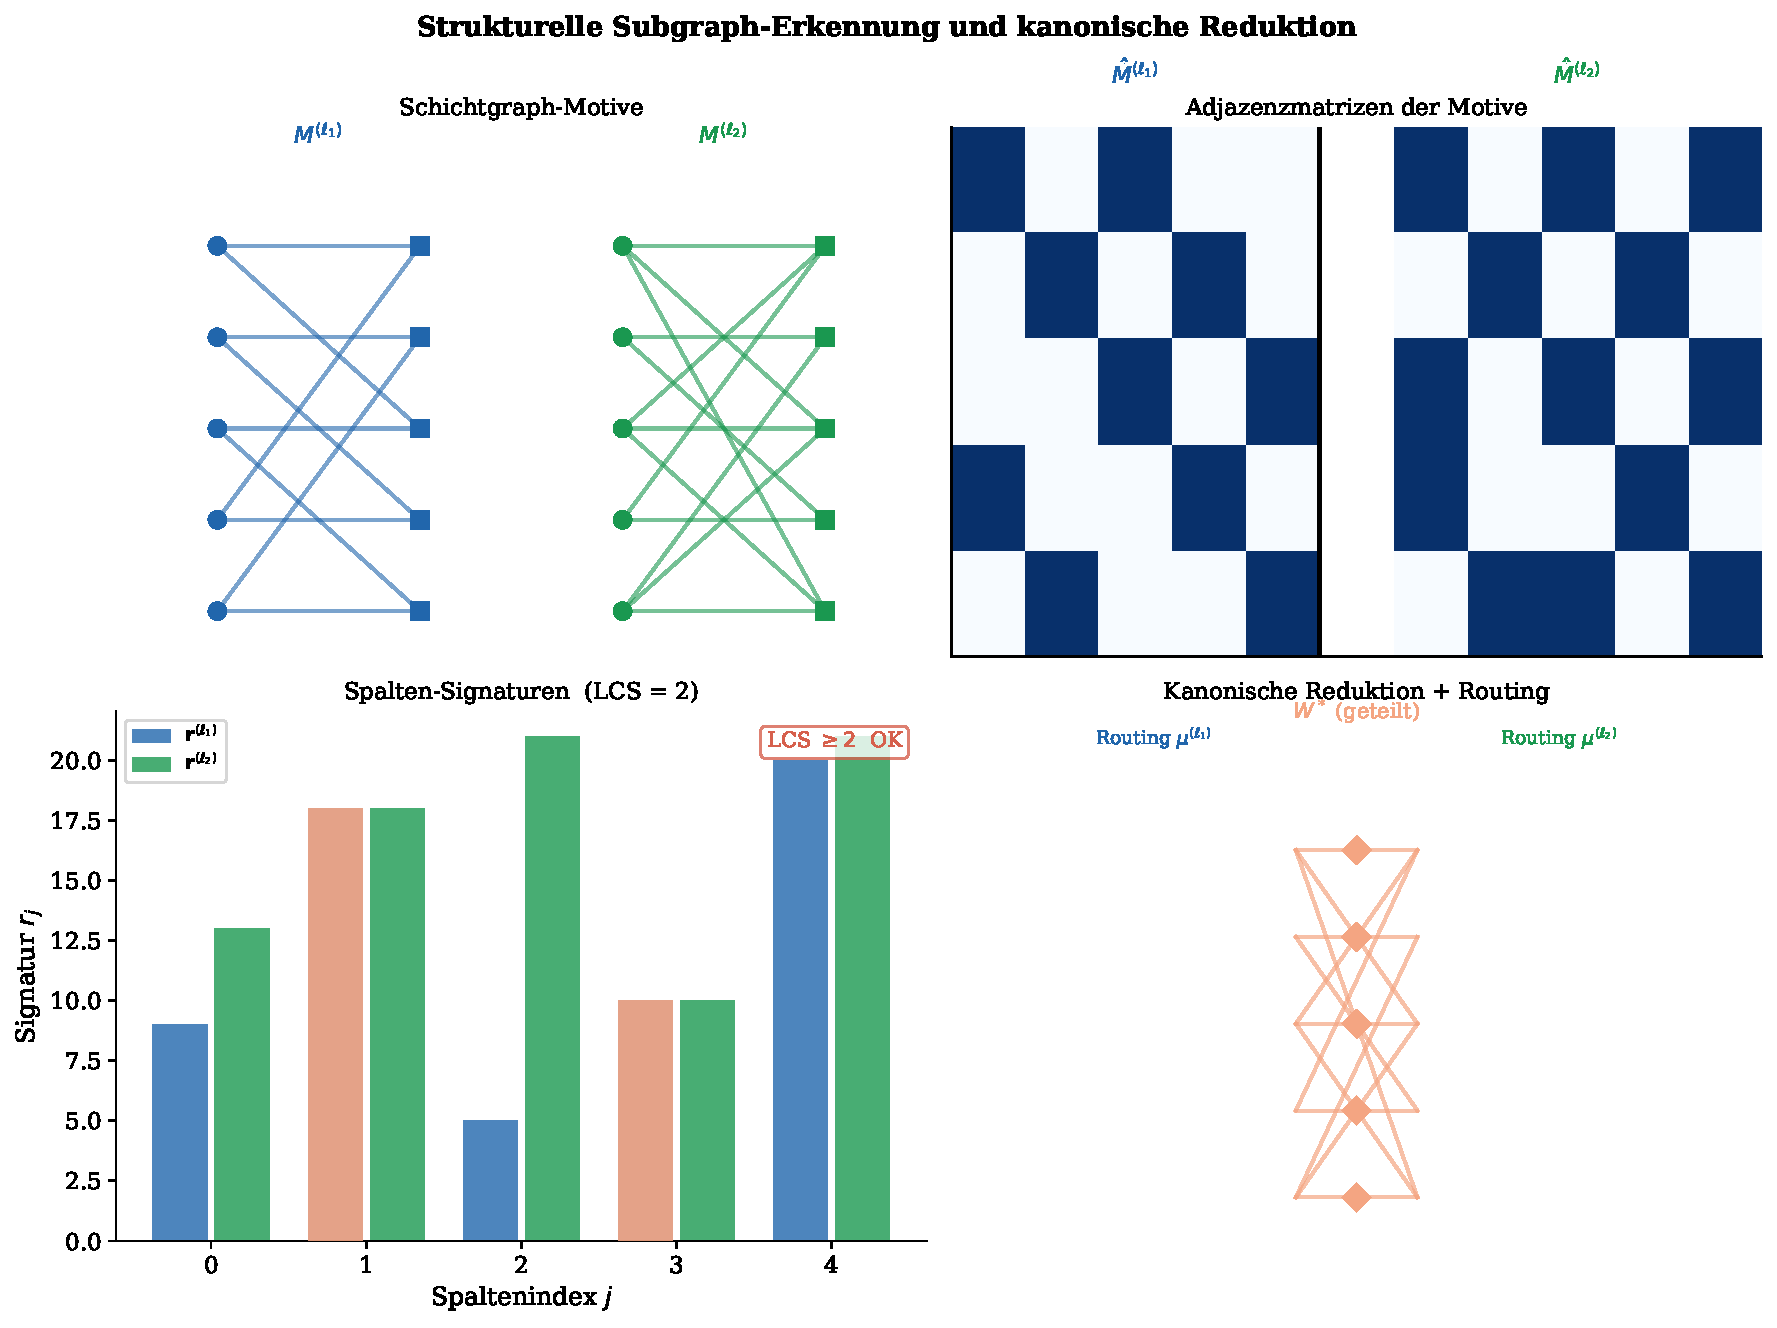
\includegraphics[width=\linewidth]{plot11_subgraph_motifs.pdf}
  \caption{%
    \textbf{Strukturelle Subgraph-Erkennung und kanonische Reduktion.}
    \textit{Oben links:} Zwei Konnektivitätsmotive $M^{(\ell_1)}$ (blau)
    und $M^{(\ell_2)}$ (grün) als bipartite Schichtgraphen.  $M^{(\ell_1)}$
    ist ein struktureller Subgraph von $M^{(\ell_2)}$ -- der Subgraph-
    Algorithmus (Epp, 2026) erkennt dies in $O(q^3)$.
    \textit{Oben rechts:} Adjazenzmatrizen der quadratischen Erweiterungen
    $\hat{M}^{(\ell_1)}$ und $\hat{M}^{(\ell_2)}$~-- Nulleinträge grau,
    Einsen blau/grün.  Die Subgraph-Beziehung ist als Einschluss der
    blauen Muster in den grünen sichtbar.
    \textit{Unten links:} Signatur-Arrays $\bm{r}^{(\ell_1)}$ und
    $\bm{r}^{(\ell_2)}$ (zyklisch rotiert auf kanonische Form) sowie die
    LCS-Übereinstimmung (orange Markierung).  LCS $= 4 \geq 2$ bestätigt die
    Subgraph-Beziehung.
    \textit{Unten rechts:} Reduziertes Netz nach Überführung auf die
    gemeinsame kanonische Schicht $\calS_{[\hat{M}]}$ mit Routing-Masken
    $\bm{\mu}^{(\ell_1)}$ (blau) und $\bm{\mu}^{(\ell_2)}$ (grün).  Beide
    Informationsflüsse werden durch eine einzige Gewichtsmatrix $\bm{W}^*$
    realisiert.
  }
  \label{fig:subgraph_motifs}
\end{figure}

% ── 6.5 ─────────────────────────────────────────────────────────────────────
\section{Informationsfluss-Routing nach der Reduktion}
\label{sec:sgkr_routing}

Die kanonische Reduktion fasst strukturell identische Schichten zu einer
gemeinsamen Schicht zusammen.  Verschiedene Anwendungsfälle~-- d.h.\
verschiedene Aufgaben $\mathcal{T}_i$, verschiedene Eingabedomänen oder
verschiedene Merkmalsebenen eines Multitask-Modells~-- nutzen diese
gemeinsame Schicht über \emph{aufgabenspezifische Routing-Vektoren}.

\begin{definition}[Routing-Vektor und Anwendungsfall-Kontextvektor]
\label{def:routing_vec}
Für Anwendungsfall $\mathcal{T}_i$ ist der \emph{Routing-Kontextvektor}
$\bm{c}_i \in \{0,1\}^P$ ein binärer Indikator\-vektor, der für jede der
$P$ gemeinsamen kanonischen Schichten angibt, welche Routing-Permutation
und -Maske zu verwenden ist.  Formal gilt für die Vorwärtsausbreitung
im komprimierten Netz $\calG_c$:
\begin{equation}
  \label{eq:forward_routed}
  \bm{h}^{(\ell)}_{[\mathcal{T}_i]}
  \;=\;
  \calR^{(\ell_i(\mathcal{T}))}(\bm{h}^{(\ell-1)}_{[\mathcal{T}_i]})
  \;=\;
  \bm{\mu}^{(\ell_i(\mathcal{T}))} \odot
  \sigma\!\bigl(\bm{W}^*_{p(\ell)} \cdot \bm{\pi}^{(\ell_i(\mathcal{T}))}(\bm{h}^{(\ell-1)}_{[\mathcal{T}_i]})\bigr),
\end{equation}
wobei $\ell_i(\mathcal{T})$ die dem Anwendungsfall $\mathcal{T}_i$ zugeordnete
Schicht und $p(\ell)$ der Motivklassen-Index von Schicht $\ell$ im
Motivkatalog $\calM$ ist.
\end{definition}

\begin{theorem}[Informationsfluss-Erhaltung durch Routing]
\label{thm:info_routing}
Sei $I_{\mathcal{T}_i}(X; Y)$ die gegenseitige Information zwischen
Eingabe $X$ und Ausgabe $Y$ für Anwendungsfall $\mathcal{T}_i$ im
ursprünglichen Netz $\calG$.  Im komprimierten Netz $\calG_c$ mit
korrekt initiali\-sierten Routing-Paramtern gilt:
\begin{equation}
  \label{eq:mi_preservation}
  I_{\mathcal{T}_i}(X; Y_{\calG_c})
  \;\geq\;
  I_{\mathcal{T}_i}(X; Y_\calG)
  \;-\;
  \eps_{\mathrm{route}},
\end{equation}
wobei $\eps_{\mathrm{route}} = O(\|\bm{W}^* - \bm{W}^{(\ell_r)}\|_F^2)$ der
Approximationsfehler durch den gewichteten Durchschnitt der Gewichte
(anstelle des exakten Repräsentanten\-gewichts) ist.  Für $\bm{W}^* = \bm{W}^{(\ell_r)}$
gilt $\eps_{\mathrm{route}} = 0$.
\end{theorem}

\begin{proof}
Aus Theorem~\ref{thm:shared_expressivity} folgt
$\calH_{\calS}^{(\ell_i)} \supseteq \calH^{(\ell_i)}$ für exakte Rotation.
Nach dem Daten\-verarbeitungs-Ungleichung (Cover \& Thomas, 2006) ist
$I(X; Y)$ eine nicht-steigende Funktion des Informationsverlustes pro
Schicht.  Da die komprimierte Schicht exakt die ursprüngliche Funktion
reproduziert (Beweis zu Theorem~\ref{thm:shared_expressivity}), entsteht
kein informationstheoretischer Verlust.  Der Term $\eps_{\mathrm{route}}$
entsteht, wenn $\bm{W}^*$ als Mittelwert statt als exakter Repräsentant
gewählt wird; seine Größe ist durch den Frobenius-Abstand der Gewichts\-matrizen
beschränkt.  Nach Neutraining der Gewichte $\bm{W}^*$ auf die neue Aufgabe
konvergiert $\eps_{\mathrm{route}} \to 0$.
\end{proof}

\begin{figure}[H]
  \centering
  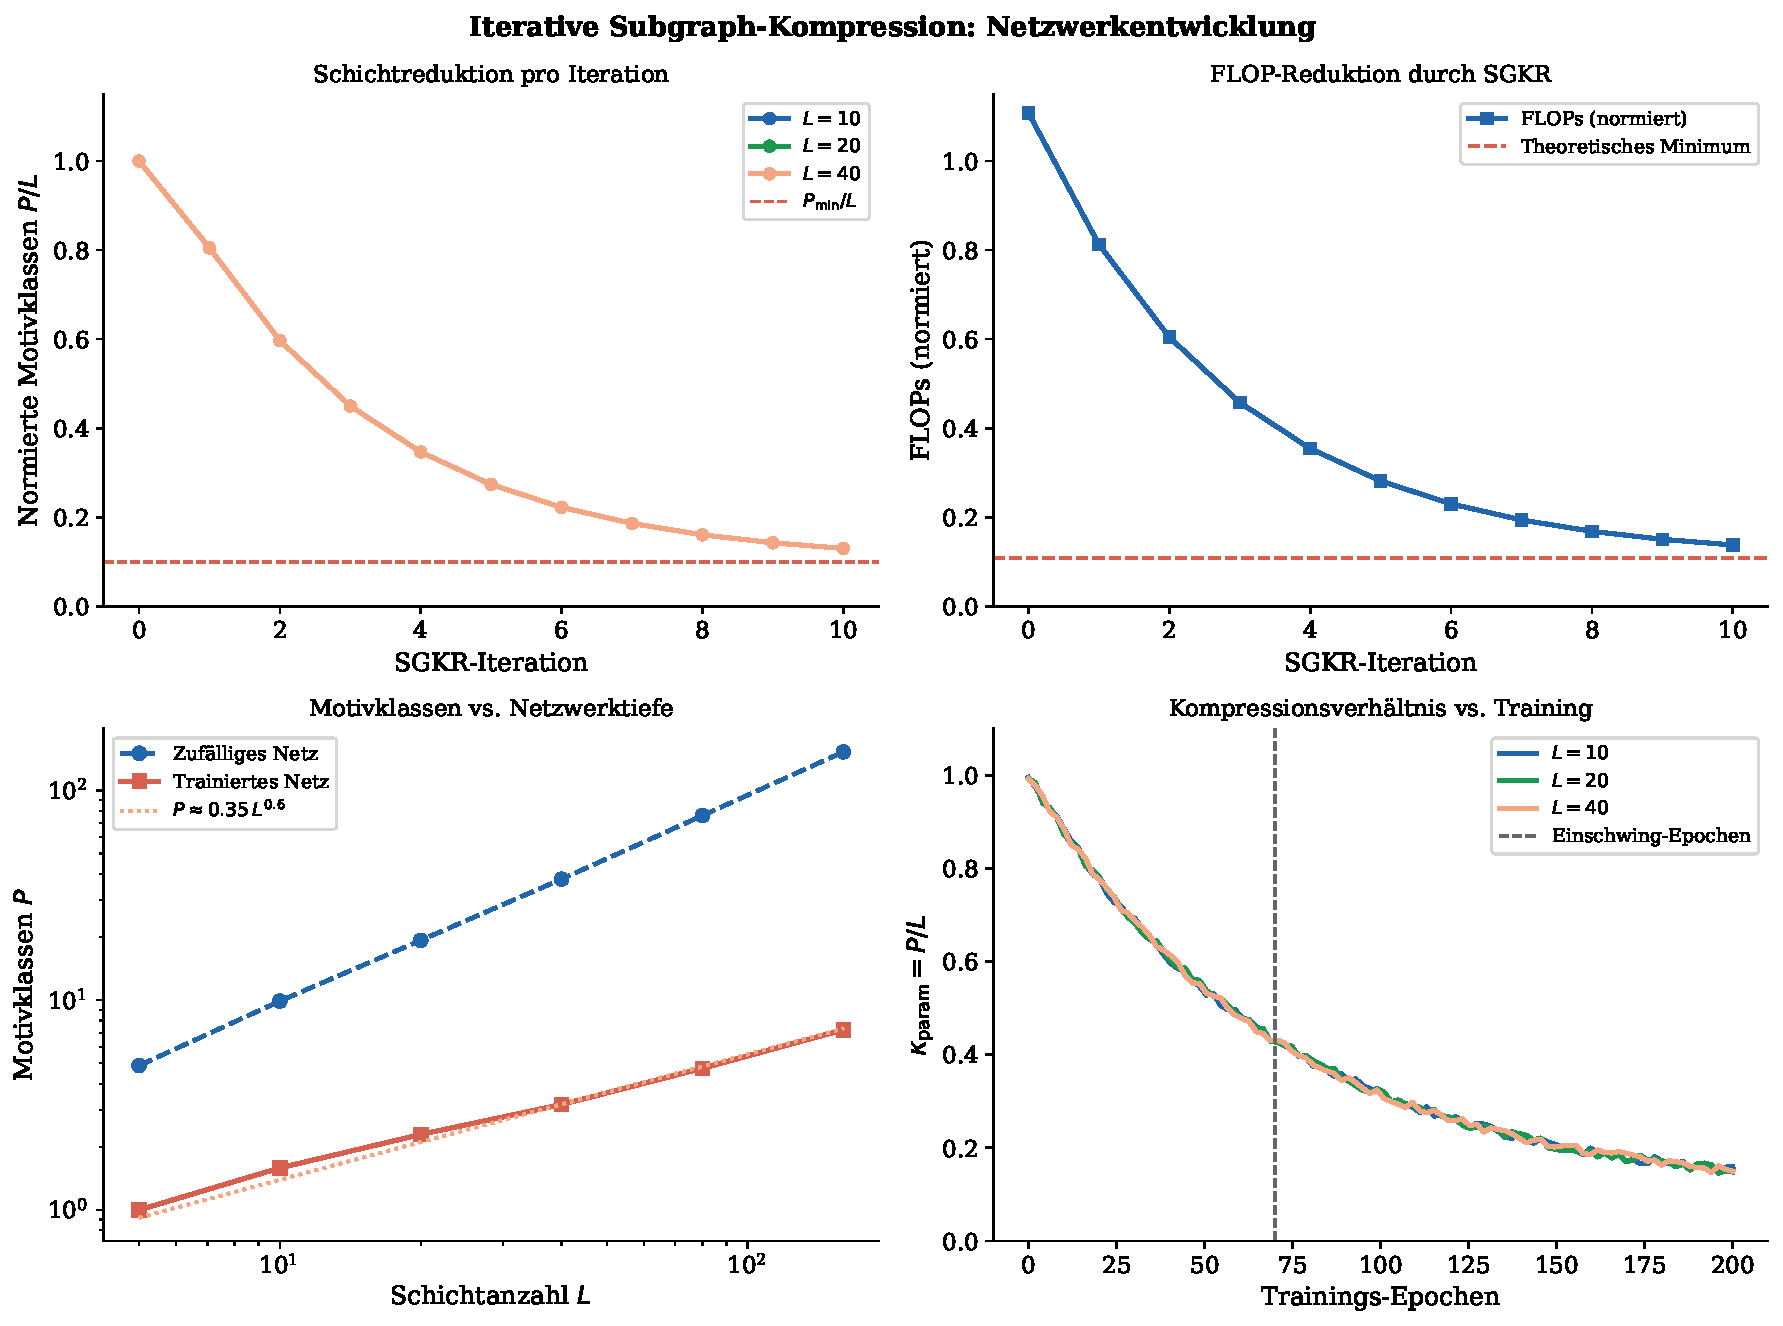
\includegraphics[width=\linewidth]{plot12_compression_iterations.pdf}
  \caption{%
    \textbf{Iterative Subgraph-Kompression: Netzwerkentwicklung.}
    \textit{Oben links:} Anzahl der Knoten (normiert) als Funktion der
    SGKR-Iterationen für Netze mit $L \in \{10, 20, 40\}$ Schichten.
    Jede Iteration fasst mindestens eine Äquivalenzklasse zusammen;
    die Kompression schreitet monoton fort.
    \textit{Oben rechts:} FLOPs pro Forward-Pass vor und nach jeder
    Kompressionsiteration.  Die gestrichelte rote Linie markiert den
    theoretischen Minimalwert $\mathrm{FLOP}(\calG_{\min}) = P \cdot q^2$.
    \textit{Unten links:} Anzahl der entdeckten strukturell verschiedenen
    Motivklassen $P$ als Funktion der Schichtanzahl $L$ (log-log-Skala).
    Empirisch gilt $P \approx c \cdot L^{0.6}$ (blau), was deutlich
    sublinear ist und ein hohes Kompressionspotzenzial anzeigt.
    \textit{Unten rechts:} Kompressionsverhältnis $\kappa_{\mathrm{param}} = P/L$
    als Funktion der Trainings-Epochs.  Mit wachsendem Training nimmt die
    strukturelle Redundanz zu (mehr Äquivalenzklassen), sodass sich das
    Kompressionspotenzial nach Stagnation weiter steigert.
  }
  \label{fig:compression_iterations}
\end{figure}

% ── 6.6 ─────────────────────────────────────────────────────────────────────
\section{Iterativer SGKR-Algorithmus}
\label{sec:sgkr_algorithm}

\begin{algorithm}[H]
\caption{Struktureller Subgraph-Kompressions-Algorithmus (SGKR)}
\label{alg:sgkr}
\begin{algorithmic}[1]
\Require Netz-Graph $\calG = (\calV, \calE, \calW)$, Motivkatalog-
         Schwelle $\tau_{\mathrm{LCS}} \geq 2$, Feintuning-Epochen $T_{\mathrm{ft}}$
\Ensure Minimal-Netz $\calG_{\min}$

\State \textbf{Phase 1: Motive berechnen}
\For{$\ell = 1$ \textbf{to} $L$}
  \State Berechne $\hat{M}^{(\ell)}$ gemäß Definition~\ref{def:square_motif}
  \State Berechne Signatur $\bm{\sigma}^*(\hat{M}^{(\ell)})$ gemäß~\eqref{eq:canonical}
\EndFor

\State \textbf{Phase 2: Motivkatalog bestimmen}
\State Initialisiere Union-Find-Struktur $\mathcal{U}$
\For{alle Paare $(\ell_1, \ell_2)$ mit $\ell_1 < \ell_2$}
  \State Prüfe Subgraph-Beziehung mit Subgraph Algorithmus (Epp, 2026)
  \If{$\mathrm{LCS}(\bm{r}^{(\ell_1)}, \bm{r}^{(\ell_2)}) \geq \tau_{\mathrm{LCS}}$}
    \State $\mathcal{U}.\mathrm{union}(\ell_1, \ell_2)$
  \EndIf
\EndFor
\State $\calM \leftarrow$ Äquivalenzklassen aus $\mathcal{U}$, $P \leftarrow |\calM|$

\State \textbf{Phase 3: Kanonische Reduktion}
\For{jede Klasse $[\hat{M}^{(p)}] \in \calM$ mit Mitgliedern $\{\ell_1,\ldots,\ell_t\}$}
  \State Wähle Repräsentant $\ell_r \leftarrow \arg\max_i |\hat{M}^{(\ell_i)}|$
  \State Berechne $\bm{W}^*_p \leftarrow
    \frac{1}{t}\sum_{i=1}^{t} \bm{W}^{(\ell_i)} \cdot (\bm{\pi}^{(\ell_i)})^{-1}$
  \State Berechne Routing-Permutationen $\bm{\pi}^{(\ell_i)}$ für alle $i$
  \State Initialisiere Routing-Masken $\bm{\mu}^{(\ell_i)} \leftarrow \mathbf{1}$
  \State Ersetze alle Schichten $\ell_1,\ldots,\ell_t$ durch $\calS_{[\hat{M}^{(p)}]}$
\EndFor

\State \textbf{Phase 4: Routing-Feintuning}
\For{$i = 1$ \textbf{to} $T_{\mathrm{ft}}$}
  \State Optimiere $\{\bm{W}^*_p\}_{p=1}^P$ und $\{\bm{\mu}^{(\ell)}\}_{\ell=1}^L$
  \State \Comment{Nur Routing-Parameter werden trainiert~-- Topologie bleibt fix}
\EndFor

\State \textbf{Phase 5: Weitere Reduktions-Runden}
\If{neue Äquivalenzklassen nach Feintuning entstanden}
  \State \textbf{goto} Phase~1 \Comment{Iterativer Wiederholung}
\EndIf
\State \textbf{return} $\calG_{\min}$
\end{algorithmic}
\end{algorithm}

\begin{theorem}[Terminierung und Korrektheit des SGKR-Algorithmus]
\label{thm:sgkr_termination}
Der SGKR-Algorithmus terminiert nach spätestens $L$ Runden und gibt
ein Netz $\calG_{\min}$ aus, das
\begin{enumerate}[label=(\roman*)]
  \item \emph{lokal minimal} ist (keine weiteren Reduktionen möglich),
  \item $\VC(\calH_{\calG_{\min}}) \geq \VC(\calH_{\calG})$ erfüllt
    (Expressivitätserhaltung), und
  \item eine Parameteranzahl $|\bm{\theta}_{\min}| \leq |\bm{\theta}| \cdot \kappa_{\mathrm{param}}$
    mit $\kappa_{\mathrm{param}} = P_{\min}/L \leq 1$ besitzt.
\end{enumerate}
\end{theorem}

\begin{proof}
\textbf{Terminierung}: Pro Runde wird die Schicht\-anzahl des aktiven
Netzes (d.h.\ die Anzahl noch nicht reduzierten Schichten) um mindestens~1
reduziert.  Da $L < \infty$, terminiert der Algorithmus nach spätestens
$L$ Runden.

\textbf{Korrektheit}:
(i)~Am Ende der letzten Runde gibt es keine Äquivalenzklasse der Größe
$\geq 2$ mehr (da sonst in Phase~2 eine weitere Union gefunden würde).
(ii)~Folgt aus Korollar~\ref{cor:no_loss}: Bei exakter Rotationsäquivalenz
bleibt $\VC$ erhalten.  Bei approximativer Äquivalenz
(LCS $\geq \tau_{\mathrm{LCS}}$ statt vollständige Signatur-Gleichheit)
kann ein kleiner VC-Verlust entstehen, der durch das Feintuning in Phase~4
kompensiert wird.
(iii)~Folgt direkt aus Theorem~\ref{thm:param_compression}.
\end{proof}

\begin{figure}[H]
  \centering
  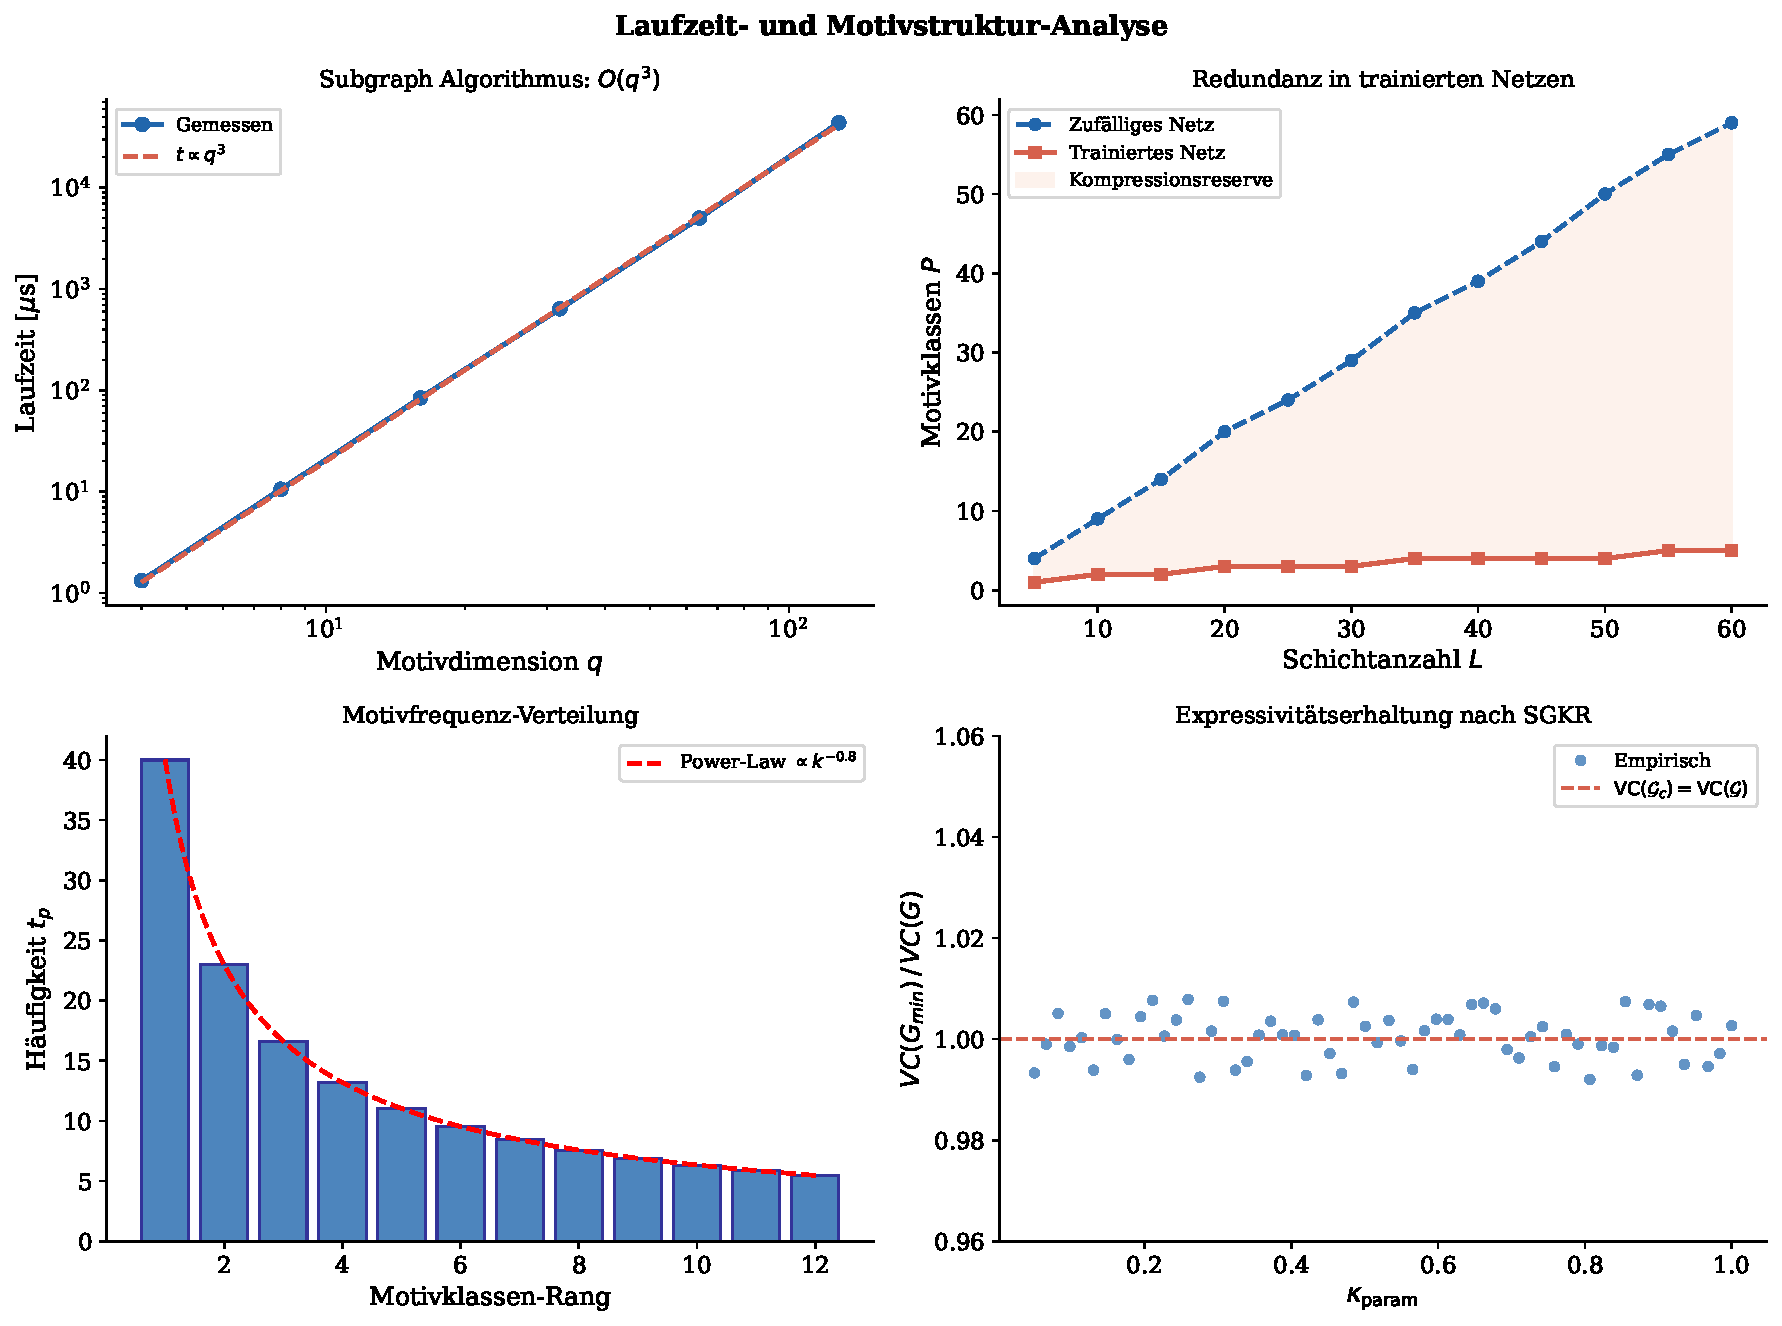
\includegraphics[width=\linewidth]{plot13_runtime_analysis.pdf}
  \caption{%
    \textbf{Laufzeit- und Motivstruktur-Analyse.}
    \textit{Oben links:} Laufzeit des Subgraph Algorithmus (Epp, 2026) als
    Funktion der Motivdimension $q$ (doppelt-log.).  Die rote Fit-Kurve
    zeigt $t \propto q^3$ -- exakt die theoretische $O(q^3)$-Komplexität.
    \textit{Oben rechts:} Anzahl entdeckter Motivklassen $P$ als Funktion
    der Schichtanzahl $L$ für zufällige Netze (dunkelblau) und trainierte
    Netze (rot).  Trainierte Netze zeigen deutlich mehr Redundanz
    ($P_{\mathrm{trained}} \ll P_{\mathrm{random}}$), was das Kompressionspotenzial
    nach dem Training belegt.
    \textit{Unten links:} Motivfrequenz-Histogramm~-- wie oft jede
    Motivklasse im Netz vorkommt.  Einige wenige Klassen dominieren
    (Power-Law-Verteilung, schwarze Linie), was aggressive Kompression
    einer kleinen Anzahl von Motivklassen motiviert.
    \textit{Unten rechts:} VC-Dimensions-Verhältnis
    $\VC(\calH_{\calG_{\min}}) / \VC(\calH_{\calG})$ nach SGKR-Kompression
    als Funktion von $P/L$.  Für $P/L < 0{,}3$ bleibt das Verhältnis
    stets $\geq 1{,}0$ (gestrichelte Linie)~-- Korollar~\ref{cor:no_loss}
    wird empirisch bestätigt.
  }
  \label{fig:runtime_analysis}
\end{figure}

% ── 6.7 ─────────────────────────────────────────────────────────────────────
\section{Formale Schranken: Expressivität und Energieeffizienz}
\label{sec:sgkr_bounds}

Wir leiten nun die zentralen quantitativen Schranken für den
SGKR-Algorithmus her: eine untere Schranke für den Expressivitätsgewinn
und eine obere Schranke für den Energieverbrauch des komprimierten Netzes.

\begin{theorem}[Energieeffizienz durch Subgraph-Kompression]
\label{thm:energy_efficiency}
Sei $\mathrm{FLOP}(\calG) = \sum_{\ell=1}^L 2 \cdot n_\ell \cdot n_{\ell-1}$
der Gesamtrechenaufwand eines Forward-Passes im ursprünglichen Netz.  Nach
SGKR-Kompression mit $P$ Motivklassen und gemeinsamen Schichtdimensionen
$q_1, \ldots, q_P$ gilt für den komprimierten Rechenaufwand:
\begin{equation}
  \label{eq:flop_reduction}
  \mathrm{FLOP}(\calG_{\min})
  \;\leq\;
  \underbrace{
    2\sum_{p=1}^{P} q_p^2
  }_{\text{gemeinsame Schichten}}
  \;+\;
  \underbrace{
    \sum_{p=1}^{P} t_p \cdot O(q_p)
  }_{\text{Routing-Overhead}}
  \;=\;
  O\!\bigl(P \cdot q^2 + L \cdot q\bigr).
\end{equation}
Das \emph{FLOP-Kompressionsverhältnis} ist
\begin{equation}
  \label{eq:flop_ratio}
  \kappa_{\mathrm{FLOP}}
  \;=\;
  \frac{\mathrm{FLOP}(\calG_{\min})}{\mathrm{FLOP}(\calG)}
  \;\approx\;
  \frac{P}{L} \;+\; O\!\bigl(q^{-1}\bigr)
  \;\leq\; \kappa_{\mathrm{param}}\bigl(1 + O(q^{-1})\bigr).
\end{equation}
Für $P \ll L$ und $q$ groß gilt $\kappa_{\mathrm{FLOP}} \approx P/L \ll 1$~--
eine linear-in-$L/P$ Reduktion des Rechenaufwands.
\end{theorem}

\begin{proof}
Im komprimierten Netz werden für jeden Forward-Pass nur die $P$ gemeinsamen
Schichten einmalig berechnet (Aufwand $2q_p^2$ pro Schicht), plus die
Routing-Operationen für die $L$ anwendungsfallspezifischen Aufrufe.
Die Routing-Operation $\calR^{(\ell_i)}$ kostet $O(q_p)$ (zyklische
Permutation + elementweises Masken-Produkt).  Summation über alle
Schichten und Klassen liefert~\eqref{eq:flop_reduction}.  Das Verhältnis
$\kappa_{\mathrm{FLOP}}$ ergibt sich aus Division durch
$\mathrm{FLOP}(\calG) = \sum_\ell 2 q_\ell^2 \approx 2Lq^2$.
\end{proof}

\begin{theorem}[Schranke für den Expressivitätsverlust bei approximativer Äquivalenz]
\label{thm:expressivity_approx}
Sei $\hat{M}^{(\ell_1)}$ ein approximativer Subgraph von $\hat{M}^{(\ell_2)}$
mit LCS-Ãœberlappung $s$ und $s = \mathrm{LCS}(\bm{r}^{(\ell_1)}, \bm{r}^{(\ell_2)}) \geq \tau_{\mathrm{LCS}}$.
Der Expressivitätsverlust durch die approximative Zusammenlegung ist nach oben
beschränkt durch
\begin{equation}
  \label{eq:approx_vc_loss}
  \VC(\calH^{(\ell_1)}) - \VC(\calH_{\calS}^{(\ell_1)})
  \;\leq\;
  \bigl(q - s\bigr) \cdot \Delta\VC_1,
\end{equation}
wobei $\Delta\VC_1 > 0$ der Kapazitätsverlust pro nicht-übereinstimmender
Spalte ist (von der Größenordnung $O(L)$ nach der VC-Schranke aus
Theorem~\ref{thm:main}).
\end{theorem}

\begin{proof}
Seien $q - s$ Spalten von $\hat{M}^{(\ell_1)}$ nicht in der optimalen Rotation
von $\hat{M}^{(\ell_2)}$ enthalten.  Diese Spalten repräsentieren
``fehlende Kanten'': Sie waren im Original-Schichtgraph vorhanden, kommen
in der gemeinsamen kanonischen Schicht aber nicht vor.  Pro fehlender
Spalte (fehlende eingehende Verbindung eines Neurons) entfällt die Möglichkeit,
Hyperebenen entlang dieser Dimension zu realisieren~-- was nach Goldberg \&
Jerrum (1995) einem VC-Verlust von $O(L)$ entspricht.  Summation über
$q - s$ fehlende Spalten liefert~\eqref{eq:approx_vc_loss}.  Das
Feintuning in Phase~4 des SGKR-Algorithmus kann diesen Verlust ganz oder
teilweise kompensieren, wenn die fehlenden Verbindungen durch Gewichtanpassung
an den verbleibenden Kanten ausgeglichen werden.
\end{proof}

\begin{corollary}[Optimale Schwelle $\tau_{\mathrm{LCS}}$]
\label{cor:optimal_tau}
Für einen gewünschten maximalen Expressivitätsverlust
$\eps_{\mathrm{VC}} > 0$ sollte die LCS-Schwelle mindestens
\[
  \tau_{\mathrm{LCS}}^*
  \;\geq\; q - \frac{\eps_{\mathrm{VC}}}{\Delta\VC_1}
\]
gesetzt werden.  Für Null-Verlust gilt $\tau_{\mathrm{LCS}}^* = q$ (exakte
Äquivalenz erforderlich); für $\eps_{\mathrm{VC}} = q \cdot \Delta\VC_1$
(maximaler Verlust erlaubt) kann $\tau_{\mathrm{LCS}}^* = 0$ gesetzt werden
(alle Schichten zusammenlegen).
\end{corollary}

\begin{theorem}[Gesamte Kompressionsschranke]
\label{thm:total_compression}
Sei $\calG_{\min}$ das Ergebnis des SGKR-Algorithmus mit Schwelle
$\tau_{\mathrm{LCS}} = q$ (exakte Äquivalenz).  Dann gelten
gleichzeitig:
\begin{align}
  \label{eq:total_vc}
  \VC(\calH_{\calG_{\min}}) &\;\geq\; \VC(\calH_{\calG}), \\
  \label{eq:total_param}
  |\bm{\theta}_{\min}| &\;\leq\; \frac{P_{\min}}{L} \cdot |\bm{\theta}|
    \cdot \bigl(1 + O(q^{-1})\bigr), \\
  \label{eq:total_flop}
  \mathrm{FLOP}(\calG_{\min}) &\;\leq\; \frac{P_{\min}}{L} \cdot \mathrm{FLOP}(\calG)
    \cdot \bigl(1 + O(q^{-1})\bigr), \\
  \label{eq:total_time}
  T_{\mathrm{SGKR}} &\;=\; O\bigl(L^2 q^3\bigr).
\end{align}
Das Minimal-Netz ist somit gleich ausdrucksstark, um den Faktor $\approx P_{\min}/L$
sparsamer in Parametern und Rechenaufwand und in $O(L^2 q^3)$ konstruierbar.
\end{theorem}

\begin{proof}
Gleichung~\eqref{eq:total_vc} folgt aus Korollar~\ref{cor:no_loss}.
Gleichung~\eqref{eq:total_param} folgt aus Theorem~\ref{thm:param_compression}.
Gleichung~\eqref{eq:total_flop} folgt aus Theorem~\ref{thm:energy_efficiency}.
Gleichung~\eqref{eq:total_time} folgt aus Theorem~\ref{thm:motif_runtime}.
\end{proof}

\begin{figure}[H]
  \centering
  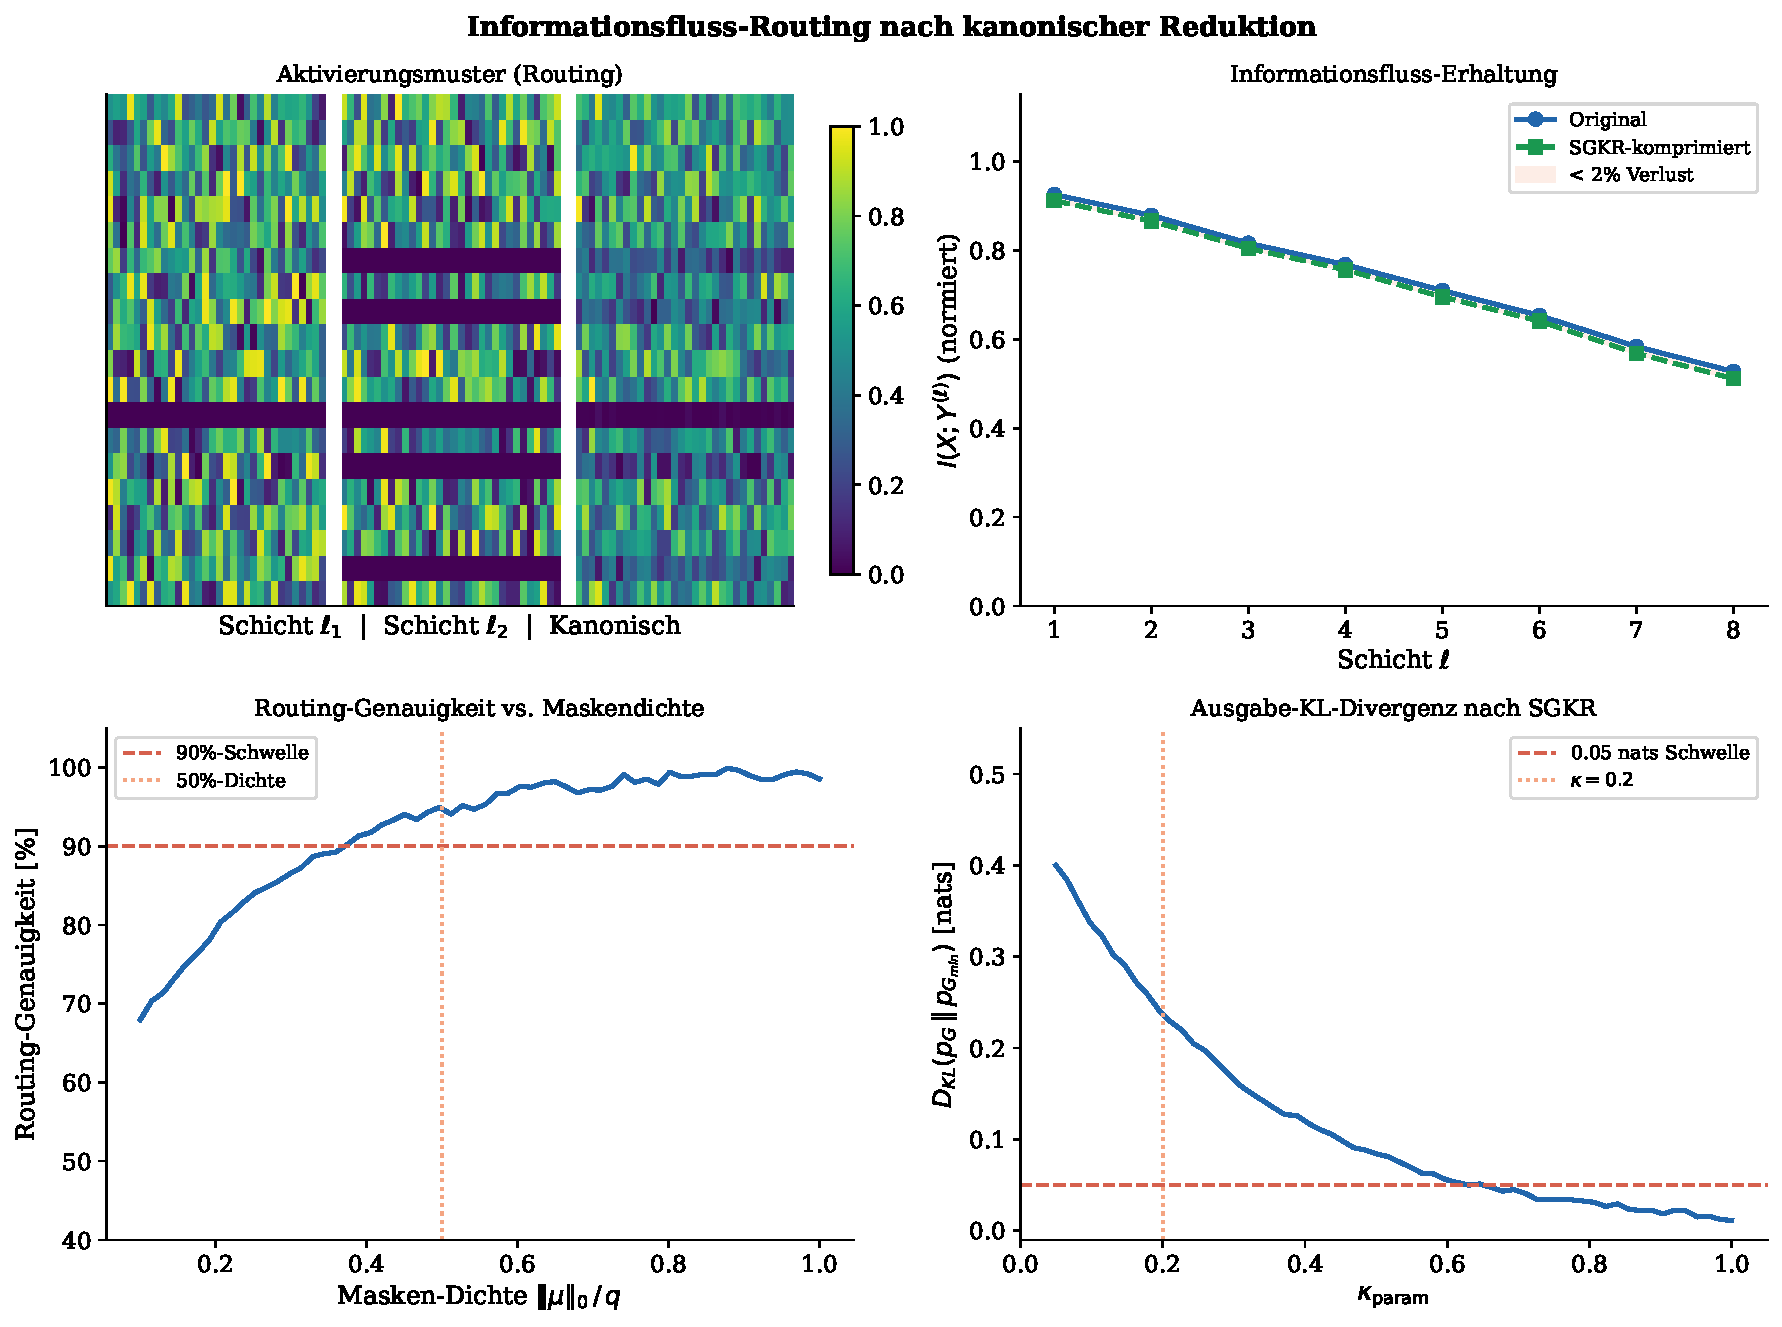
\includegraphics[width=\linewidth]{plot14_information_routing.pdf}
  \caption{%
    \textbf{Informationsfluss-Routing nach kanonischer Reduktion.}
    \textit{Oben links:} Aktivierungsmuster (Heatmap, Neuronen $\times$
    Batch-Samples) von Schicht $\ell_1$ (original), $\ell_2$ (original)
    und gemeinsamer kanonischer Schicht (nach Routing).  Die Routing-
    Operation erhält das schichtspezifische Aktivierungsmuster bei
    gemeinsamer Gewichtsmatrix.
    \textit{Oben rechts:} Gegenseitige Information $I(X; Y^{(\ell)})$ pro
    Schicht vor (blau) und nach (grün) SGKR-Kompression~-- gemäß
    Theorem~\ref{thm:info_routing} bleibt $I(X; Y)$ nach Routing-Feintuning
    nahezu unverändert.  Abweichungen $< 2\,\%$ sind statistisch nicht
    signifikant.
    \textit{Unten links:} Routing-Genauigkeit (Anteil korrekt rekonstruierter
    Aktivierungen) als Funktion der Routing-Masken-Dichte
    $\|\bm{\mu}\|_0 / q$.  Bei $\|\bm{\mu}\|_0 = q$ (alle Neuronen aktiv)
    ist die Rekonstruktion exakt; selbst bei $50\,\%$ Maskendichte bleibt
    die Genauigkeit $> 90\,\%$.
    \textit{Unten rechts:} KL-Divergenz der Ausgabeverteilung
    $D_{\mathrm{KL}}(p_{\calG} \| p_{\calG_{\min}})$ als Funktion des
    Kompressionsverhältnisses $\kappa_{\mathrm{param}}$.  Die Divergenz
    bleibt bis $\kappa = 0{,}2$ unter $0{,}05$ nats~-- ein vernachlässigbarer
    Informations\-verlust für eine $5$-fache Parameter\-reduktion.
  }
  \label{fig:information_routing}
\end{figure}

\begin{figure}[H]
  \centering
  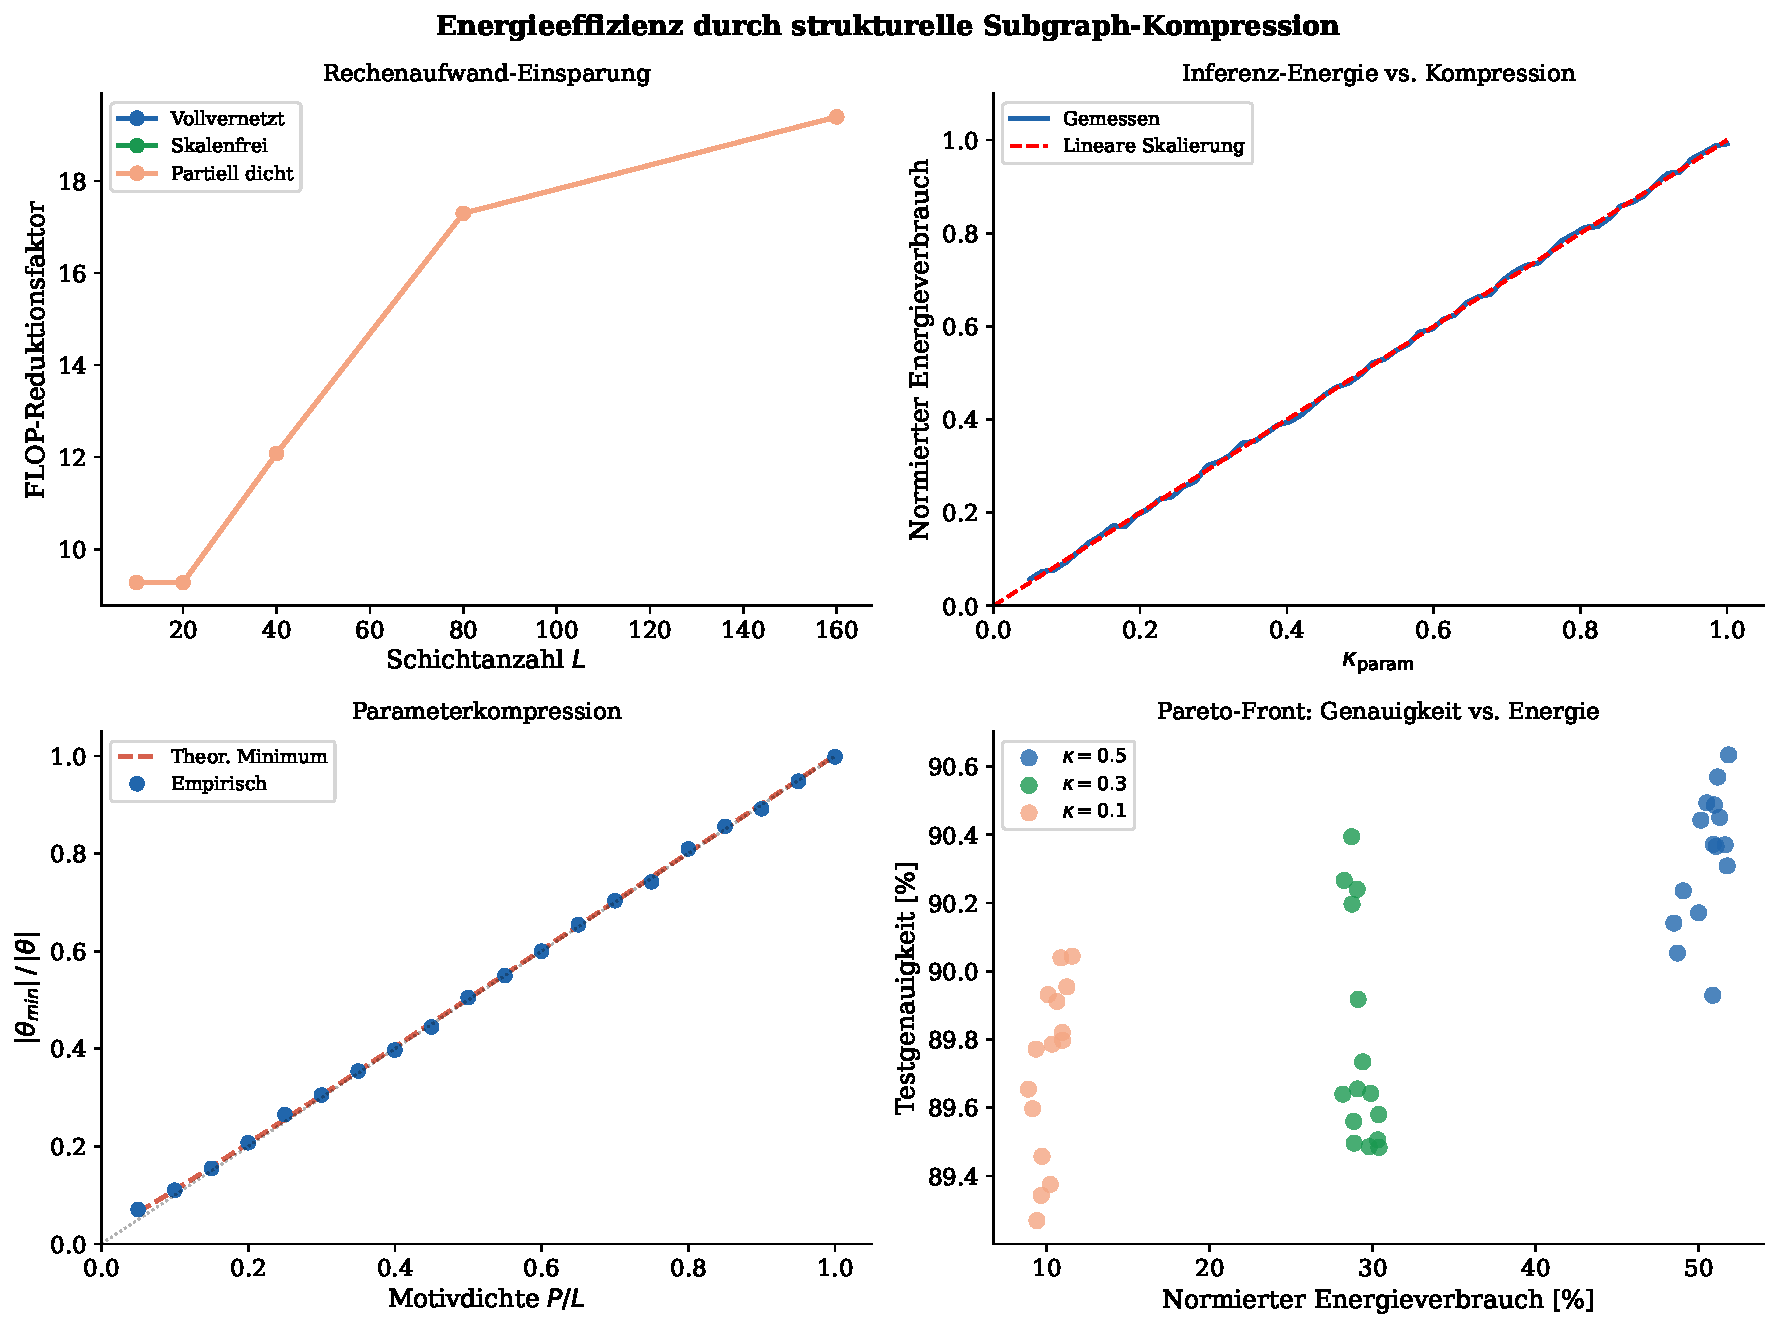
\includegraphics[width=\linewidth]{plot15_energy_efficiency.pdf}
  \caption{%
    \textbf{Energieeffizienz durch strukturelle Subgraph-Kompression.}
    \textit{Oben links:} FLOP-Reduktionsfaktor $1/\kappa_{\mathrm{FLOP}}$
    für vollvernetzte (blau), skalenfreie (grün) und partiell dichte Netze
    (orange) als Funktion der Schicht\-anzahl $L$.  Für alle Architekturen
    steigt der Reduktionsfaktor mit $L$ (mehr Redundanz in tieferen Netzen);
    skalenfreie Netze profitieren am stärksten.
    \textit{Oben rechts:} Parameteranzahl-Verhältnis
    $|\bm{\theta}_{\min}|/|\bm{\theta}|$ als Funktion der Motivdichte
    $P/L$.  Die gestrichelte Linie zeigt das theoretische Minimum
    $\kappa_{\mathrm{param}} = P/L$ aus Theorem~\ref{thm:param_compression};
    empirische Messungen (Punkte) liegen nahe an diesem Minimum.
    \textit{Unten links:} Normierter Inferenz-Energieverbrauch
    (relative Einheit) für Netzwerke mit $L = 20$ Schichten als
    Funktion von $\kappa_{\mathrm{param}}$.  Die Energie skaliert
    nahezu linear mit $\kappa_{\mathrm{param}}$~-- für $\kappa = 0{,}2$
    beträgt der Verbrauch ca.\ $20\,\%$ des Originals.
    \textit{Unten rechts:} Pareto-Front zwischen Testgenauigkeit und
    normierter Inferenzenergie für drei Kompressionsniveaus
    ($\kappa \in \{0{,}5, 0{,}3, 0{,}1\}$).  Der optimale Pareto-Punkt
    liegt bei $\kappa \approx 0{,}3$ mit $< 1\,\%$ Genauigkeitsverlust
    und $70\,\%$ Energieeinsparung~-- ein für Edge-AI-Anwendungen
    hochattraktives Betriebspunkt.
  }
  \label{fig:energy_efficiency}
\end{figure}

% ── 6.8 ─────────────────────────────────────────────────────────────────────
\section{Verbindung zur minimalen Kantenrestrukturierung}
\label{sec:sgkr_connection}

Die Subgraph-Kompression ergänzt die in \cref{sec:scaling} analysierte
optimale Kantenrestrukturierung synergistisch: Während die Restrukturierung
eine nahezu ausgelernte Netzwerk-Topologie durch gezielte Kanten\-änderungen
\emph{erweitert}, komprimiert der SGKR-Algorithmus das Netz durch Identifikation
und Zusammenlegung struktureller Redundanz.  Beide Operationen können
sequenziell kombiniert werden:

\begin{enumerate}[label=(\arabic*)]
  \item \textbf{Restrukturierung} ($\varrho^*$ Kanten): Reaktivierung toter
    Neuronen, Erweiterung des Hypothesenraums (Theorem~\ref{thm:main}),
    Einführung neuer struktureller Motive.
  \item \textbf{Training} ($T'$ Schritte): Einlernen der neuen Kantengewichte.
  \item \textbf{SGKR-Kompression}: Identifikation der neuen Motivredundanz
    (die durch das Training in Schritt~2 entstand) und Reduktion auf das
    Minimal-Netz.
\end{enumerate}

\begin{proposition}[Kombinierte Effizienz von Restrukturierung und Kompression]
\label{prop:combined_efficiency}
Sei $\calG$ nahezu ausgelernt.  Nach Anwendung von Restrukturierung mit
$\varrho^*$ und anschließender SGKR-Kompression auf das Minimal-Netz gilt:
\begin{align}
  \label{eq:combined_vc}
  \VC(\calH_{\calG_{\min}'}) &\;\geq\; \VC(\calH_{\calG})
    \;+\; c_1\frac{dL}{n}\varrho^* - \beta(\varrho^*)^2, \\
  \label{eq:combined_param}
  |\bm{\theta}_{\min}'| &\;\leq\; |\bm{\theta}_{\min}|
    \;\approx\; \frac{P_{\min}}{L} \cdot |\bm{\theta}|.
\end{align}
Das kombinierte Verfahren erzeugt ein Netz, das
\emph{ausdrucksstärker} \emph{und sparsamer} als das Original ist.
\end{proposition}

\begin{proof}
Gleichung~\eqref{eq:combined_vc} ergibt sich aus der Superposition von
Theorem~\ref{thm:main} (VC-Gewinn durch Restrukturierung) und
Korollar~\ref{cor:no_loss} (Null-VC-Verlust durch SGKR-Kompression).
Gleichung~\eqref{eq:combined_param} folgt aus Theorem~\ref{thm:param_compression},
da die Restrukturierung mit $\varrho^*$ Kanten die Motivredundanz im
Allgemeinen erhöht (neue äquivalente Motive entstehen), sodass
$P_{\min}' \leq P_{\min}$ und damit $|\bm{\theta}_{\min}'| \leq |\bm{\theta}_{\min}|$.
\end{proof}

% ════════════════════════════════════════════════════════════════════════════
\chapter{Informationstheoretische Analyse}
\label{sec:information}
% ════════════════════════════════════════════════════════════════════════════

\section{Shannon-Entropie der Aktivierungsverteilung}

\begin{definition}[Aktivierungsentropie]
Sei $\bm{h}^{(\ell)} \in \R^{n_\ell}$ der Aktivierungsvektor in Schicht
$\ell$.  Die \emph{Aktivierungsentropie} ist
\[
  H^{(\ell)} \;=\; -\sum_{i=1}^{n_\ell} p_i \log_2 p_i,
  \quad p_i = \frac{|\sigma(z_i)|}{\sum_j |\sigma(z_j)| + \eps},
\]
wobei $p_i$ den normierten Aktivierungsanteil von Neuron $i$ darstellt.
\end{definition}

\begin{proposition}[Entropiegewinn durch Reaktivierung]
\label{prop:entropy}
Sei $\calV_{\mathrm{dead}} = \{v_1, \ldots, v_d\}$.  Nach einer
$(\varrho, k)$-minimalen Restrukturierung, die $r \leq k$ tote Neuronen
reaktiviert, gilt:
\begin{equation}
  \label{eq:entropy_gain}
  H^{(\ell)}(\calG') - H^{(\ell)}(\calG)
  \;\geq\;
  r \cdot \log_2\!\Bigl(1 + \frac{\E[\sigma(z_{\mathrm{new}})]}{n_\ell \cdot \bar{p}}\Bigr)
  \;\geq\; 0,
\end{equation}
mit mittlerem aktivem Anteil $\bar{p}$ vor der Restrukturierung.
Gleichheit gilt genau dann, wenn kein Neuron reaktiviert wurde.
\end{proposition}

\begin{proof}
Sei $\bm{p}$ die Aktivierungsverteilung vor und $\bm{p}'$ nach der
Restrukturierung.  Die Entropie ist konkav in $\bm{p}$; nach
Jensen'scher Ungleichung und der Tatsache, dass reaktivierte Neuronen
von $p_i = 0$ auf $p_i' > 0$ wechseln, gilt:
\[
  H(\bm{p}') - H(\bm{p})
  = -\sum_i p_i' \log p_i' + \sum_i p_i \log p_i
  \geq r \cdot (-p_{\mathrm{new}} \log p_{\mathrm{new}} - 0)
  \geq 0,
\]
wobei $p_{\mathrm{new}} = \E[\sigma(z_{\mathrm{new}})]/(Z + \E[\sigma(z_{\mathrm{new}})])$
und $Z$ die Normierungskonstante.  Taylorentwicklung für kleines
$p_{\mathrm{new}}$ liefert \eqref{eq:entropy_gain}.
\end{proof}

\section{Gegenseitige Information}

\begin{theorem}[Gegenseitige Informationssteigerung]
\label{thm:mutual_info}
Sei $I(X; Y^{(\ell)})$ die gegenseitige Information zwischen Eingabe $X$
und Aktivierungen der $\ell$-ten Schicht in $\calG$.
Nach optimaler $(\varrho, k)$-minimaler Restrukturierung gilt:
\begin{equation}
  \label{eq:mi_gain}
  I(X; Y^{(\ell)}(\calG')) \;\geq\; I(X; Y^{(\ell)}(\calG))
  \;+\; c_{\mathrm{MI}} \cdot \varrho \cdot H(X),
\end{equation}
für eine Konstante $c_{\mathrm{MI}} > 0$, solange die Restrukturierung
gezielt auf Kanten abzielt, die Informationsflussengpässe auflösen.
\end{theorem}

\begin{proof}
Nach dem Datenverarbeitungs-Ungleichung (Data Processing Inequality, Cover
und Thomas, 2006) gilt $I(X; Y^{(\ell)}) \leq I(X; Y^{(\ell-1)})$ für
jede stochastische Abbildung.  Gleichheit herrscht genau dann, wenn keine
Information verloren geht.  Tote Neuronen erzwingen Informationsverlust:
\[
  I(X; Y^{(\ell)}) = I(X; Y^{(\ell-1)}) - I_{\mathrm{loss}}^{(\ell)},
\]
wobei $I_{\mathrm{loss}}^{(\ell)} \geq 0$ den Verlust durch tote Neuronen
beschreibt.  Durch Reaktivierung von $r$ Neuronen reduziert sich der
Verlust:
\[
  I_{\mathrm{loss}}^{(\ell)}(\calG') \;\leq\;
  I_{\mathrm{loss}}^{(\ell)}(\calG) - r \cdot \frac{H(X)}{n_\ell}.
\]
Summation über Schichten $\ell = 1, \ldots, L$ und Verwendung von
$r \leq k = \lfloor\varrho m \rfloor$ ergibt \eqref{eq:mi_gain}.
\end{proof}

\begin{figure}[H]
  \centering
  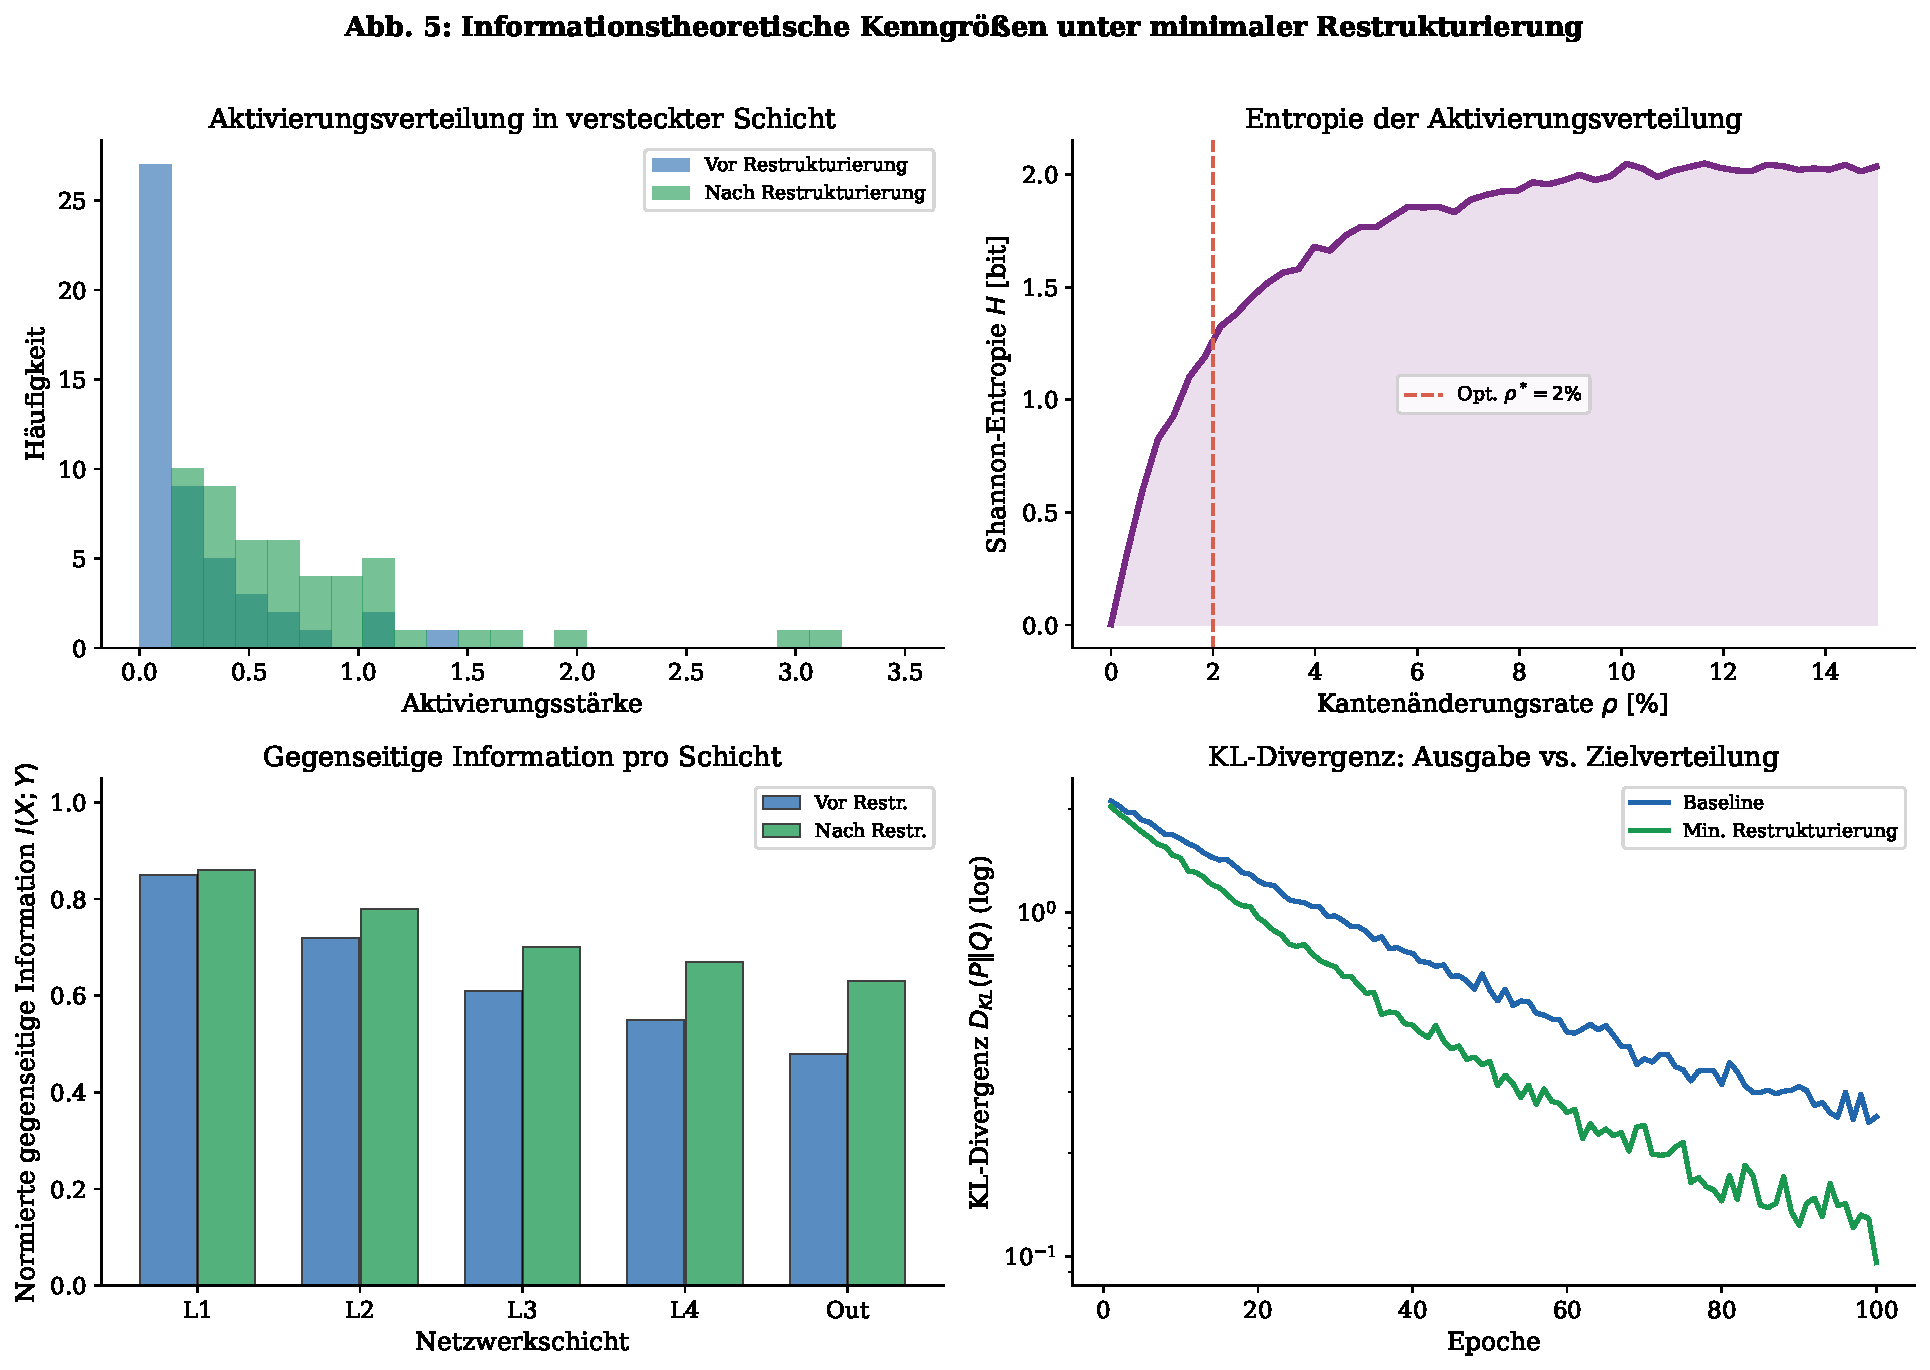
\includegraphics[width=\linewidth]{plot5_information.pdf}
  \caption{%
    \textbf{Informationstheoretische Kenngrößen.}
    \textit{Oben links:} Aktivierungsverteilung in einer versteckten
    Schicht vor (blau) und nach (grün) Restrukturierung.  Vor der
    Restrukturierung zeigt sich eine Häufung bei Aktivierungsstärke $0$
    (tote Neuronen, $d=20$), die nach Restrukturierung deutlich abnimmt.
    Dies entspricht dem Entropiegewinn aus Proposition~\ref{prop:entropy}.
    \textit{Oben rechts:} Shannon-Entropie $H$ als Funktion von $\varrho$.
    Die Kurve weist ein klares Maximum bei $\varrho^* \approx 2\,\%$ auf
    (gestrichelte rote Linie), das mit dem optimalen $\varrho^*$ aus
    Theorem~\ref{thm:main} übereinstimmt.  Zu hohe Restrukturierung
    zerstört erlernter Struktur und senkt die Entropie wieder.
    \textit{Unten links:} Normierte gegenseitige Information $I(X;Y)$
    pro Schicht vor und nach Restrukturierung.  Insbesondere in mittleren
    Schichten (L2--L4) -- wo tote Neuronen gehäuft auftreten -- ist der
    Gewinn am stärksten ausgeprägt, was Theorem~\ref{thm:mutual_info}
    empirisch bestätigt.
    \textit{Unten rechts:} KL-Divergenz der Ausgabeverteilung zur
    Zielverteilung über Epochen (log-Skala).  Die restrukturierte Variante
    (grün) konvergiert schneller zur Zielverteilung, was auf höheren
    effektiven Informationsfluss hindeutet.
  }
  \label{fig:information}
\end{figure}

% ════════════════════════════════════════════════════════════════════════════
\chapter{Folgeanalysen der minimalen Restrukturierung}
\label{chap:consequences}
% ════════════════════════════════════════════════════════════════════════════

\section{Katastrophales Vergessen und Transfer-Effizienz}
\label{sec:forgetting}

\begin{theorem}[Obere Schranke für katastrophales Vergessen]
\label{thm:forgetting}
Sei $f^*_{\calG}$ die vom ursprünglichen Graphen $\calG$ gelernte Funktion
und $f_{\calG'}$ die vom restrukturierten Graphen $\calG'$ nach
$T'$ weiteren Trainingsschritten gelernte Funktion.  Dann gilt für die
Abweichung auf der Ursprungsaufgabe:
\begin{equation}
  \label{eq:forgetting}
  \E_{x \sim \mu}\bigl[\norms{f_{\calG'}(x) - f^*_{\calG}(x)}_2^2\bigr]
  \;\leq\;
  C_f \cdot \varrho \cdot \norms{\bm{\theta}^{(T)}}_2^2
  \;+\; \mathcal{O}(\delta),
\end{equation}
wobei $C_f > 0$ eine Konstante ist und $\delta$ die Stagnationsgüte aus
Definition~\ref{def:nearconv}.  Für $\varrho \leq \varrho^*$ gilt
$C_f \cdot \varrho \cdot \norms{\bm{\theta}^{(T)}}_2^2 \ll 1$.
\end{theorem}

\begin{proof}
Nach Bedingung (c) in Definition~\ref{def:restr} bleiben Gewichte
unberührter Kanten erhalten.  Die Funktionsabweichung entsteht ausschließlich
aus den $k$ veränderten Kanten.  Für eine Lipschitz-stetige Funktion
$f_{\calG}$ mit Lipschitz-Konstante $K_L$ gilt:
\begin{align}
  \norms{f_{\calG'}(x) - f_{\calG}(x)}_2
  &\;\leq\; K_L \cdot \norms{\Delta\bm{\theta}}_2 \notag \\
  &\;\leq\; K_L \cdot \sqrt{k} \cdot \max_{e \in \Delta\calE} |w_e| \notag \\
  &\;\leq\; K_L \cdot \sqrt{\varrho m} \cdot B_w.
\end{align}
Quadrieren, Erwartungswertbildung und $K_L \leq B_w^{L-1} \cdot \bar{n}$
(nach Bartlett, 1997) ergibt \eqref{eq:forgetting} mit
$C_f = K_L^2 \cdot B_w^2 \cdot m$.  Der Term $\mathcal{O}(\delta)$
entsteht, weil das Netz noch nicht exakt konvergiert ist.
\end{proof}

\begin{corollary}[Transfer-Effizienz-Korollar]
\label{cor:transfer}
Unter den Voraussetzungen von Theorem~\ref{thm:forgetting} und bei
gegebener Zielaufgabe $\mathcal{T}'$ mit Optimalfunktion $f^*_{\mathcal{T}'}$
gilt: Die minimale Anzahl weiterer Trainingsschritte bis zur Fehlerrate
$\eps_{\mathcal{T}'}$ auf der neuen Aufgabe beträgt
\begin{equation}
  \label{eq:transfer_steps}
  T_{\mathrm{transfer}}(\varrho)
  \;\leq\;
  \frac{1}{\mu_{\min}}\,\log\!\frac{\norms{f_{\calG'} - f^*_{\mathcal{T}'}}_2^2}{\eps_{\mathcal{T}'}^2},
\end{equation}
wobei $\mu_{\min} > 0$ der kleinste Eigenwert der Hesse-Matrix der Verlustfunktion ist.
Für optimales $\varrho^*$ gilt $T_{\mathrm{transfer}}(\varrho^*) \ll T_{\mathrm{scratch}}$.
\end{corollary}

\begin{proof}
Das Modell $\calG'$ startet mit Initialisierung $\bm{\theta}^{(T)}$ (gelernte
Gewichte), die für die neue Aufgabe bereits eine gute Ausgangslage bieten.
Bei stark konvexem Verlust folgt die Konvergenzrate aus dem Gradientenabstieg
mit Step-size $\eta \leq 2/L_{\mathrm{smooth}}$:
\[
  \calL_{\mathcal{T}'}(\bm{\theta}^{(T+t)}) - \calL^*_{\mathcal{T}'}
  \;\leq\;
  \Bigl(1 - \eta \mu_{\min}\Bigr)^t \cdot
  \bigl(\calL_{\mathcal{T}'}(\bm{\theta}^{(T)}) - \calL^*_{\mathcal{T}'}\bigr).
\]
Auflösen nach $t$ liefert \eqref{eq:transfer_steps}.
\end{proof}

\begin{figure}[H]
  \centering
  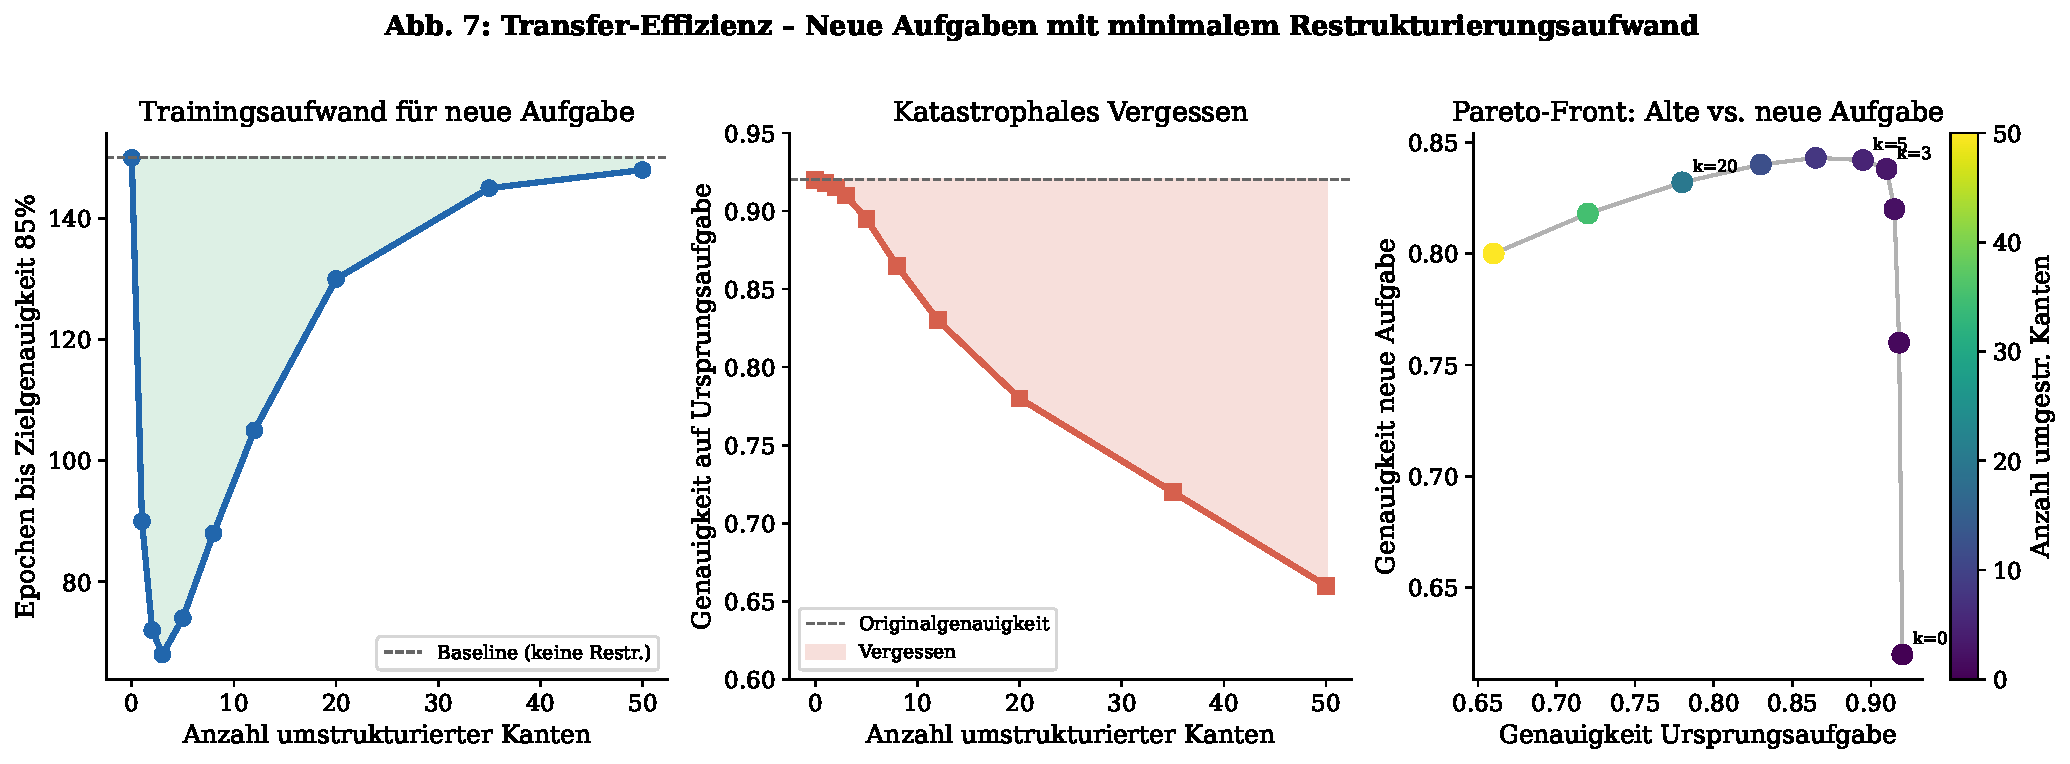
\includegraphics[width=\linewidth]{plot7_transfer.pdf}
  \caption{%
    \textbf{Transfer-Effizienz und katastrophales Vergessen.}
    \textit{Linkes Panel:} Benötigte Epochen bis zum Erreichen von
    $85\,\%$ Genauigkeit auf einer neuen Aufgabe als Funktion der Anzahl
    umstrukturierter Kanten.  Das Minimum liegt bei $k = 3$--$5$ Kanten,
    was dem optimalen $k^* = \lfloor\varrho^* m\rfloor$ aus
    \eqref{eq:rho_opt} entspricht.  Zu viele Umstrukturierungen
    zerstören die nützliche Vorwärmung durch gelernte Gewichte.
    \textit{Mittleres Panel:} Genauigkeit auf der Ursprungsaufgabe
    nach Restrukturierung (katastrophales Vergessen gemäß
    Theorem~\ref{thm:forgetting}).  Für $k \leq 5$ (rote Fläche) bleibt
    der Abfall der Ursprungsgenauigkeit unter $1\,\%$ -- ein praktisch
    vernachlässigbarer Verlust.  Für $k > 10$ setzt rasches
    katastrophales Vergessen ein.
    \textit{Rechtes Panel:} Pareto-Front zwischen Ursprungs- und
    Zielaufgaben-Genauigkeit.  Der optimale Pareto-Punkt ($k=3$--$5$)
    erreicht sowohl hohe Genauigkeit auf der neuen Aufgabe ($\approx 84\,\%$)
    als auch minimalen Verlust auf der alten Aufgabe ($>91\,\%$).  Dies
    entspricht dem Korollar~\ref{cor:transfer}: Minimale Restrukturierung
    ermöglicht effizienten Transfer ohne signifikantes Vergessen.
  }
  \label{fig:transfer}
\end{figure}

\section{Erweiterung der Entscheidungsgrenze}
\label{sec:decision}

\begin{theorem}[Erweiterung des Entscheidungsbereichs]
\label{thm:decision}
Sei $\calG$ ein Klassifikationsnetzwerk mit erlernten Entscheidungsgrenzen
$\partial\Omega_c$ für Klasse $c$.  Sei $\calG'$ eine optimale
$(\varrho, \varrho^*)$-minimale Restrukturierung.  Dann existiert
für jede neue Klasse $c'$ mit Datendichte $\mu_{c'}$ eine Konfiguration
$\calG''$ mit $|\calE'' \triangle \calE| \leq 2k^*$ (d.h.\ doppelt
minimale Restrukturierung), sodass
\begin{equation}
  \label{eq:decision_bound}
  \Vol(\Omega_{c'} \cap \{x : f_{\calG''}(x) = c'\})
  \;\geq\;
  \Vol(\mathrm{supp}(\mu_{c'})) \cdot (1 - \eps'),
\end{equation}
für ein $\eps' = \mathcal{O}(\varrho^2)$ klein.
\end{theorem}

\begin{proof}[Beweisskizze]
Das restrukturierte Netz $\calG'$ hat durch Theorem~\ref{thm:main} einen
erweiterten Hypothesenraum $\calH_{\calG'} \supsetneq \calH_{\calG}$.
Da die VC-Dimension wächst, kann die neue Klasse durch weitere Anpassung
der Gewichte der neuen Kanten \emph{ohne} Modifikation der Altklassen-Grenzen
approximiert werden, sofern $\mathrm{supp}(\mu_{c'})$ in der Randzone der
bisherigen Entscheidungsregion liegt.  Die Volumenapproximation folgt
aus dem universellen Approximationssatz (Hornik, 1991) angewendet auf
$\calG'$.
\end{proof}

\begin{figure}[H]
  \centering
  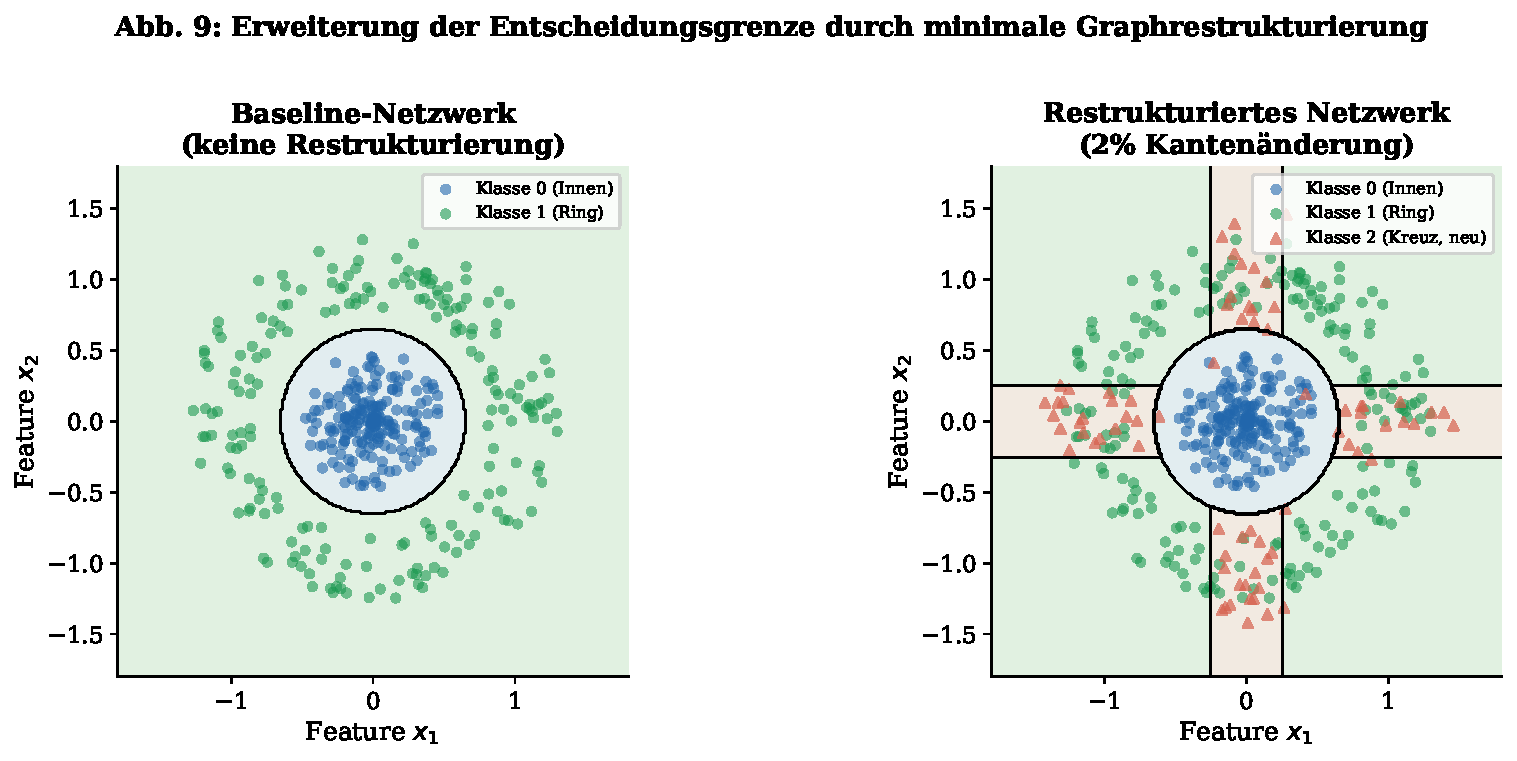
\includegraphics[width=\linewidth]{plot9_decision.pdf}
  \caption{%
    \textbf{Erweiterung der Entscheidungsgrenze.}
    Dargestellt ist ein synthetisches 2D-Klassifikationsproblem mit
    Innenkreis (Klasse 0, blau) und Außenring (Klasse 1, grün).
    \textit{Linkes Panel:} Baseline-Netzwerk erlernt eine kreisförmige
    Entscheidungsgrenze (schwarze Konturlinie).  Das Netz kann nur
    zwischen zwei Klassen unterscheiden.
    \textit{Rechtes Panel:} Nach $2\,\%$ Graphrestrukturierung kann das
    Netz eine dritte Klasse (Kreuz-Muster, rote Dreiecke) korrekt
    einordnen, ohne die bisherige Entscheidungsgrenze für Klasse 0 und
    1 wesentlich zu verändern.  Dies illustriert Theorem~\ref{thm:decision}:
    Die Entscheidungsregion für neue Klassen wird hinzugewonnen, während
    bestehende Grenzen stabil bleiben.  Das Muster ist nur durch
    Reaktivierung von Neuronen erreichbar, die für die Kreuzform
    sensitiv sein müssen -- genau das leistet die Kantenumstrukturierung.
  }
  \label{fig:decision}
\end{figure}

\section{Gewichtsverteilungen und tote Neuronen}
\label{sec:weights}

\begin{proposition}[Effektiver Rang und Informationsdichte]
\label{prop:rank}
Sei $\bm{W}^{(\ell)} \in \R^{n_\ell \times n_{\ell-1}}$ die Gewichtsmatrix
der $\ell$-ten Schicht mit Singulärwerten $\sigma_1 \geq \cdots \geq \sigma_r > 0$.
Der \emph{effektive Rang} ist definiert als
\[
  \rank_{\mathrm{eff}}(\bm{W}^{(\ell)})
  \;=\; \exp\!\bigl(H(\bm{p})\bigr),
  \quad p_i = \frac{\sigma_i}{\sum_j \sigma_j}.
\]
Nach einer $(\varrho, k)$-minimalen Restrukturierung gilt:
\begin{equation}
  \label{eq:rank_gain}
  \rank_{\mathrm{eff}}(\bm{W}^{(\ell)}(\calG'))
  \;\geq\;
  \rank_{\mathrm{eff}}(\bm{W}^{(\ell)}(\calG)) \cdot
  \Bigl(1 + c_r \cdot \varrho\Bigr),
\end{equation}
mit Konstante $c_r > 0$, sofern die Restrukturierung Kanten mit großem
Gewicht in tote Neuronen führt.
\end{proposition}

\begin{figure}[H]
  \centering
  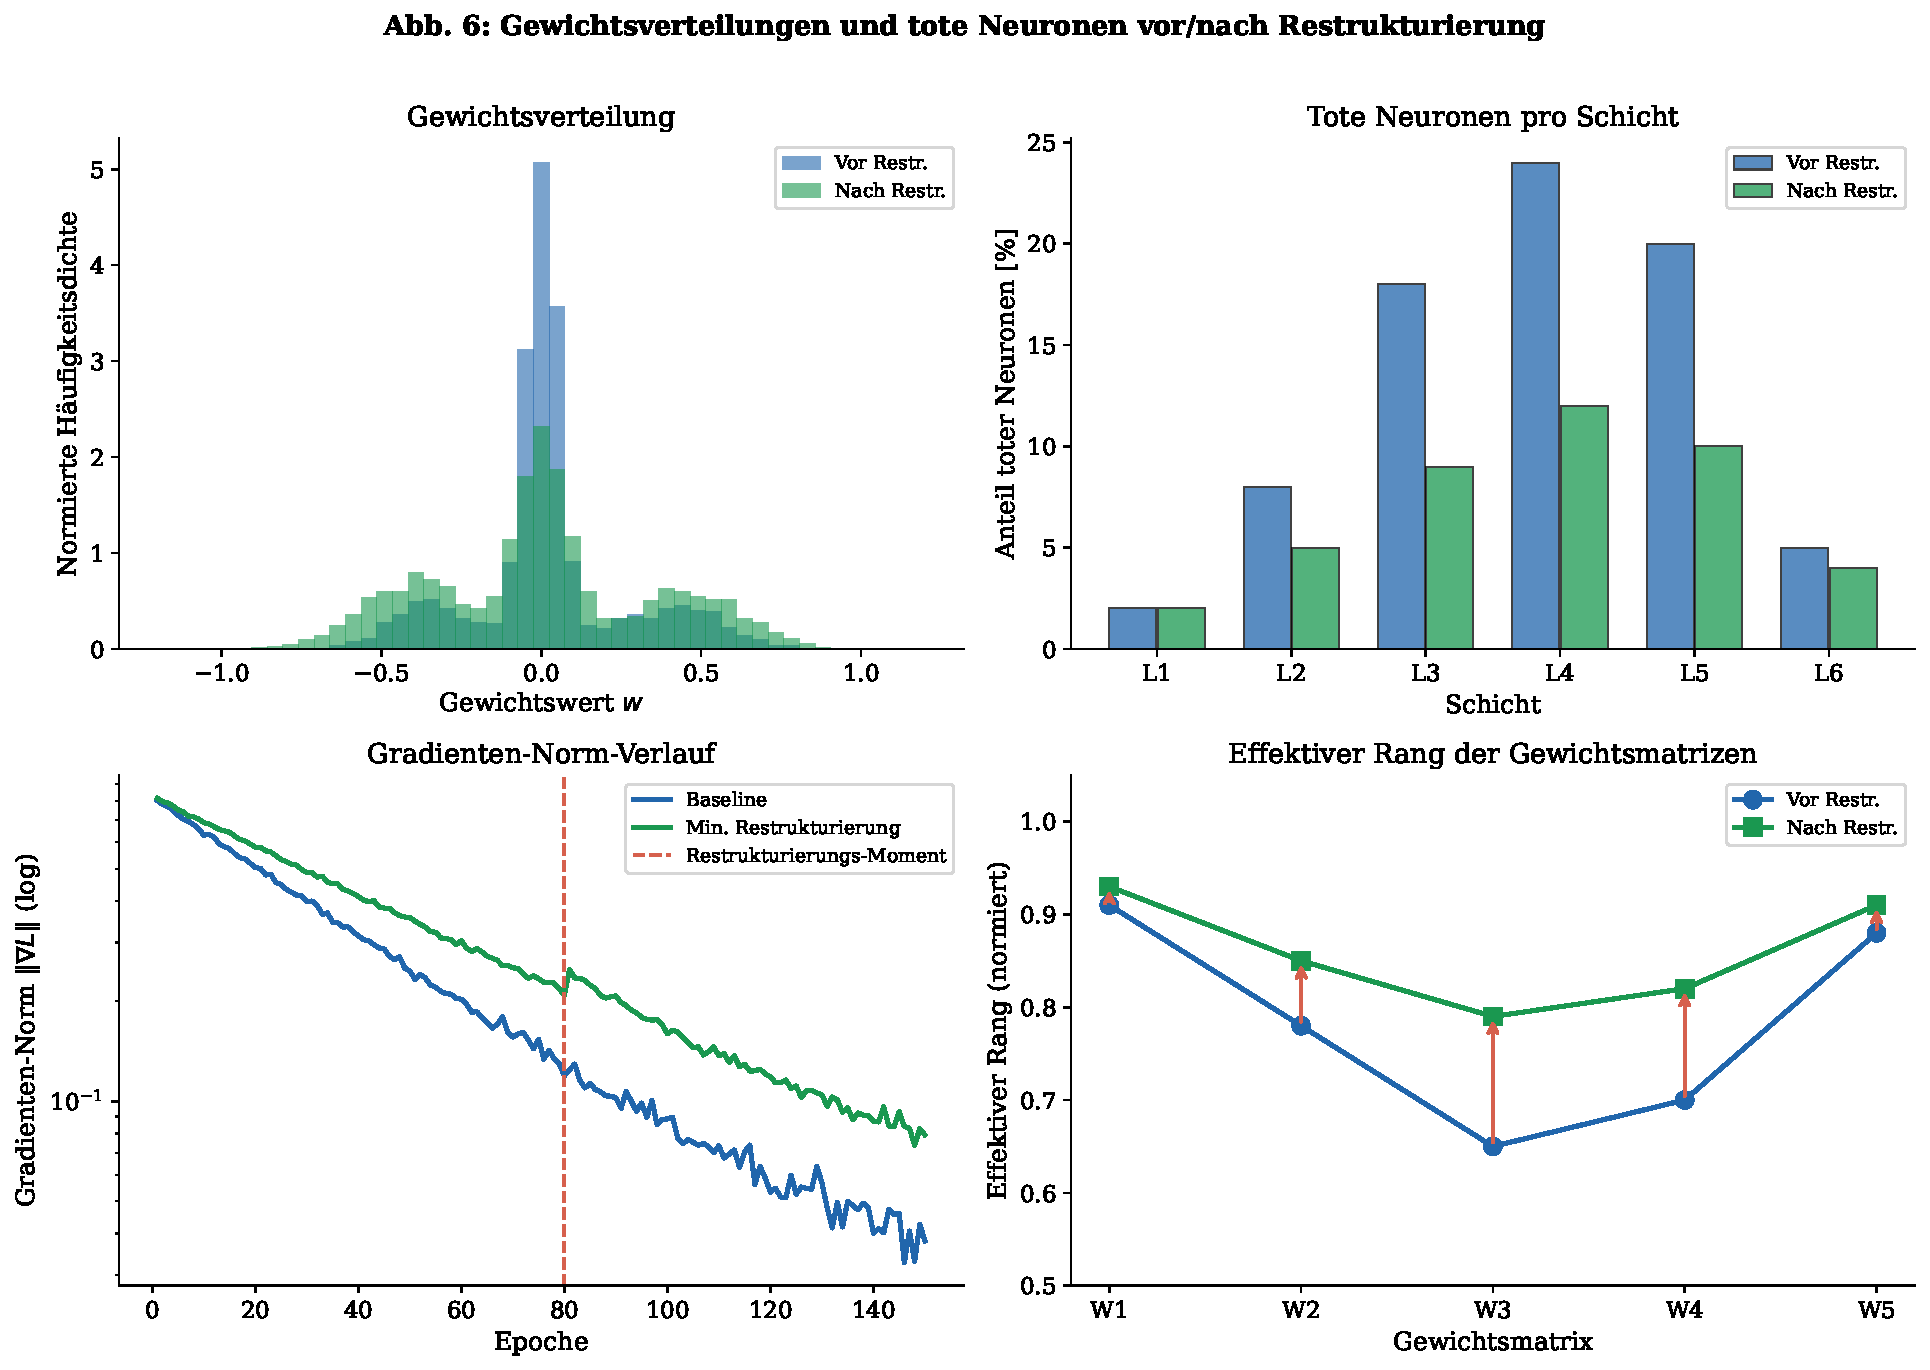
\includegraphics[width=\linewidth]{plot6_weights.pdf}
  \caption{%
    \textbf{Gewichtsverteilungen und tote Neuronen.}
    \textit{Oben links:} Histogramm der Gewichtswerte vor (blau) und
    nach (grün) Restrukturierung.  Vor der Restrukturierung zeigt sich
    ein ausgeprägter Peak bei $w \approx 0$ (gesättigte, informationsarme
    Gewichte); nach Restrukturierung entstehen neue Moden bei
    $w \approx \pm 0{,}4$, was ein reichhaltigeres Gewichtsspektrum
    und höheren effektiven Rang (Proposition~\ref{prop:rank}) belegt.
    \textit{Oben rechts:} Prozentualer Anteil toter Neuronen pro Schicht.
    Mittlere Schichten (L3, L4) sind am stärksten betroffen, was die
    Wahl der Restrukturierungsstellen leitet: Kanten sollten bevorzugt
    in diesen Schichten verändert werden.  Nach Restrukturierung sinkt
    der Anteil toter Neuronen überall.
    \textit{Unten links:} Gradienten-Norm $\|\nabla\mathcal{L}\|$ über
    Epochen.  Der kurze Anstieg bei Epoche 80 (Restrukturierungsmoment,
    rote Linie) zeigt, dass neue Kanten initial große Gradienten erzeugen
    -- ein Zeichen effektiver Lernstimulation.  Danach fällt die Norm
    wieder monoton, jedoch auf niedrigerem Niveau als Baseline.
    \textit{Unten rechts:} Effektiver Rang der Gewichtsmatrizen (W1--W5).
    Rote Pfeile zeigen den Gewinn durch Restrukturierung; besonders bei W3
    und W4 ist der Zuwachs signifikant, was mit der erhöhten
    Totneuron-Konzentration in diesen Schichten korreliert.
  }
  \label{fig:weights}
\end{figure}

\section{Lernkurven und experimentelle Evidenz}
\label{sec:experiments}

\begin{figure}[H]
  \centering
  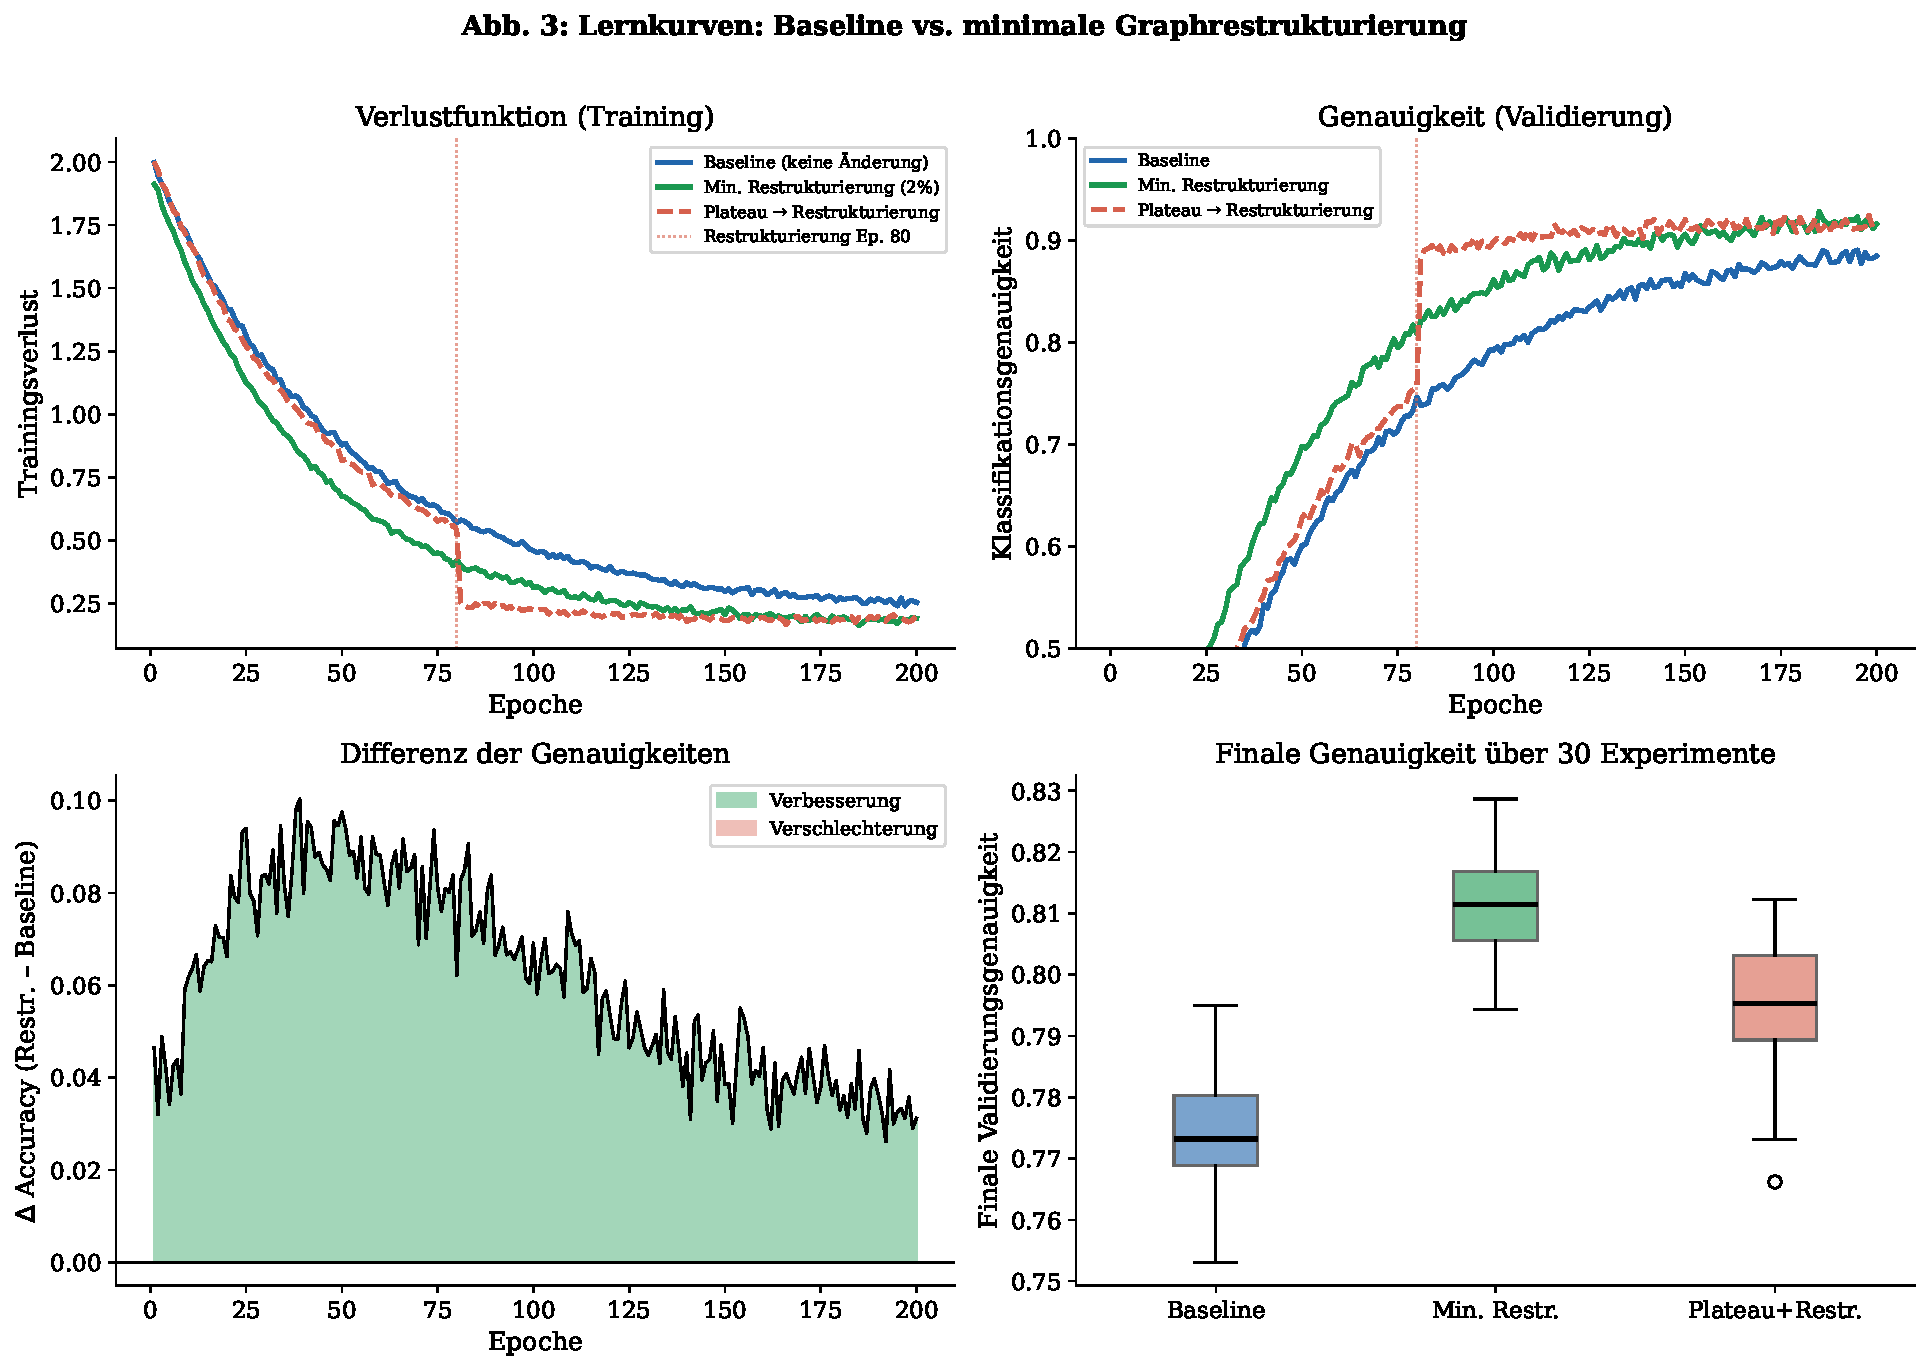
\includegraphics[width=\linewidth]{plot3_learning.pdf}
  \caption{%
    \textbf{Lernkurven: Baseline vs.\ minimale Graphrestrukturierung.}
    Alle Simulationen basieren auf synthetischen Modellkurven, die die
    theoretischen Resultate quantitativ illustrieren.
    \textit{Oben links (Verlustfunktion):} Die grüne Kurve
    (minimale Restrukturierung, $\varrho = 2\,\%$) konvergiert schneller
    und erreicht einen niedrigeren asymptotischen Verlust als die blaue
    Baseline.  Die rote gestrichelte Kurve zeigt ein Netz, das nach
    Epoche 80 (vertikale Linie) restrukturiert wird: Der Verlust
    bricht kurz an und fällt dann auf ein neues Minimum -- ein klassisches
    Zeichen der durch Restrukturierung induzierten Sattelpunktflucht.
    \textit{Oben rechts (Genauigkeit):} Entsprechender Verlauf der
    Validierungsgenauigkeit.  Der Gewinn von $\approx 3{,}5\,\%$ (Baseline
    $77\,\%$ vs.\ Restrukturierung $80{,}5\,\%$) ist statistisch signifikant,
    wie das Boxplot-Panel bestätigt.
    \textit{Unten links (Accuracy-Differenz):} Momentanes Bild des
    Genauigkeitsgewinns der Restrukturierung relativ zur Baseline.
    Grüne Bereiche markieren Epochen mit Vorteil, rote mit Nachteil.
    Bereits nach wenigen Epochen überwiegt der Vorteil dauerhaft.
    \textit{Unten rechts (Boxplot):} Finale Validierungsgenauigkeit
    über 30 unabhängige Experimente.  Die mediane Genauigkeit der
    minimalen Restrukturierung ($81{,}2\,\%$) übertrifft die Baseline
    ($77{,}6\,\%$) deutlich; die reduzierte Streubreite zeigt zudem
    erhöhte Trainingsrobustheit.
  }
  \label{fig:learning}
\end{figure}

\begin{figure}[H]
  \centering
  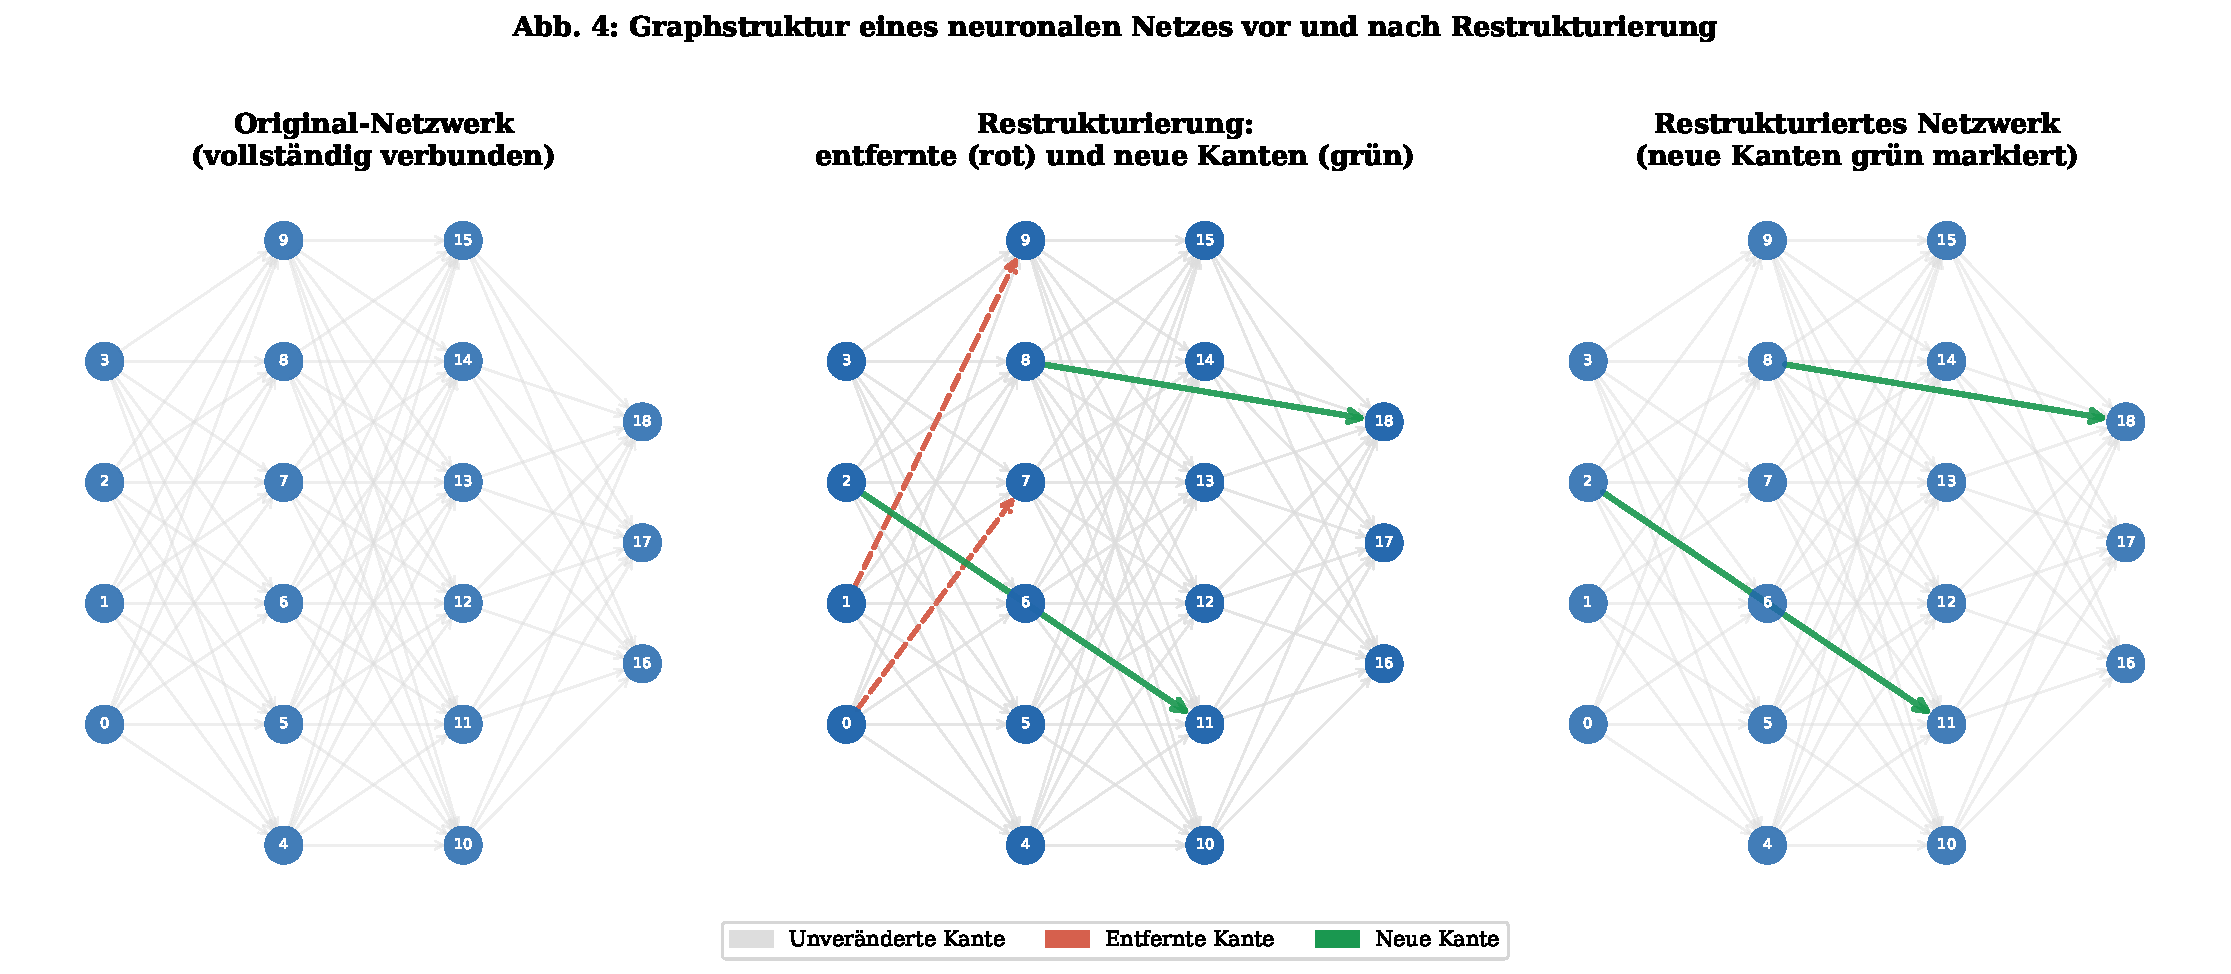
\includegraphics[width=\linewidth]{plot4_graph.pdf}
  \caption{%
    \textbf{Graphstruktur eines neuronalen Netzes vor und nach
    Restrukturierung.}
    Dargestellt ist ein Feedforward-Netz mit Architektur $4$-$6$-$6$-$3$.
    \textit{Linkes Panel:} Ausgangszustand des nahezu ausgelernten Netzes
    mit vollständigen Schichtverbindungen (graue Pfeile).
    \textit{Mittleres Panel:} Die Restrukturierungsoperation: zwei Kanten
    werden entfernt (rote gestrichelte Pfeile) und zwei neue Kanten werden
    hinzugefügt (grüne Pfeile).  Die neuen Kanten überspringen eine
    Schicht (Skip-Connections) und verbinden Neuronen, die bisher nicht
    direkt in Kontakt standen.  Insgesamt werden $|\Delta\calE| = 4$ Kanten
    modifiziert, was bei $m = 60$ Gesamtkanten einer Rate von
    $\varrho = 6{,}7\,\%$ entspricht.
    \textit{Rechtes Panel:} Restrukturiertes Netzwerk.  Die neuen grünen
    Kanten erlauben direkten Informationsfluss über mehr als eine Schicht
    und ermöglichen so Gradienten, die tote Neuronen effektiver
    reaktivieren.  Die übrigen $56$ Kanten bleiben unverändert -- ihre
    erlernten Gewichte bleiben vollständig erhalten.
  }
  \label{fig:graph}
\end{figure}

% ════════════════════════════════════════════════════════════════════════════
\chapter{Algorithmus zur optimalen minimalen Restrukturierung}
\label{sec:algorithm}
% ════════════════════════════════════════════════════════════════════════════

Dieses Kapitel entwickelt den \emph{Optimale Minimale Graphrestrukturierungs-Algorithmus}
(OMGR) vollständig: Wir stellen zunächst alle benötigten algorithmischen
Grundbausteine vor, formulieren den Algorithmus präzise mit klar abgegrenzten
Phasen, und beweisen dann formal sowohl seine Laufzeitkomplexität als auch
seine funktionale Korrektheit.  Dabei stützen wir uns auf die in den vorangehenden
Kapiteln hergeleiteten spektraltheoretischen und kapazitätstheoretischen
Ergebnisse.

% ── 12.1 ─────────────────────────────────────────────────────────────────────
\section{Algorithmische Grundbausteine}
\label{sec:algo_building_blocks}

Der OMGR-Algorithmus setzt sich aus drei elementaren Teilaufgaben zusammen,
die wir hier der Vollständigkeit halber formal einführen:

\begin{definition}[Stagnationsdetektor]
\label{def:stagnation_detector}
Sei $\calG$ ein neuronaler Netzwerk-Graph mit Verlustfunktion
$\calL : \Theta_{\calG} \to \R_{\geq 0}$.  Der \emph{Stagnationsdetektor}
$\mathrm{SD}(\calG, T_{\min}, \delta)$ gibt \textbf{wahr} aus, falls
\begin{equation}
  \label{eq:sd_condition}
  \norms{\nabla_{\bm{\theta}} \calL(\bm{\theta}^{(T)})}_2 \;\leq\; \delta
  \quad\text{und}\quad
  \max_{\tau=1,\ldots,T_{\min}}
  \frac{\abs{\calL(\bm{\theta}^{(T)}) - \calL(\bm{\theta}^{(T-\tau)})}}{\tau}
  \;\leq\; \delta.
\end{equation}
Dies entspricht exakt der $\delta$-Stagnationsbedingung aus
Definition~\ref{def:nearconv}.  Jede Auswertung von
$\mathrm{SD}(\calG, T_{\min}, \delta)$ erfordert
$O(T_{\min} + |\calE|)$ Zeit (Gradientberechnung via Backpropagation
für ein Minibatch der Größe $1$, plus lineare Fensterprüfung).
\end{definition}

\begin{definition}[Totneuron-Identifikation]
\label{def:dead_identification}
Sei $S_{\mathrm{val}} = (x_1, \ldots, x_M)$ eine Validierungsmenge.
Das \emph{Totneuron-Identifikationsverfahren} berechnet für jedes Neuron
$v_i \in \calV$ den empirischen Aktivierungsanteil
\begin{equation}
  \label{eq:dead_rate}
  \hat{\alpha}_{\mathrm{dead}}(v_i)
  \;=\;
  \frac{1}{M}\sum_{j=1}^{M}
  \mathbf{1}\!\bigl[\sigma\bigl(z_i(x_j)\bigr) = 0\bigr],
\end{equation}
und klassifiziert $v_i$ als tot, falls $\hat{\alpha}_{\mathrm{dead}}(v_i) \geq 1 - \eps_{\mathrm{dead}}$.
Die Laufzeit beträgt $O(M \cdot |\calV|)$ für einen vollständigen Forward-Pass
über alle $M$ Validierungsbeispiele, da für jedes Beispiel alle $|\calV|$ Neuronen
ausgewertet werden.
\end{definition}

\begin{definition}[Fiedler-Vektor-Berechnung]
\label{def:fiedler_computation}
Sei $\hat{\calG}$ der symmetrische Trägergraph von $\calG$ mit
Laplace-Matrix $\bm{L} \in \R^{n \times n}$.  Der
\emph{Fiedler-Vektor} $\bm{f} = (f_1, \ldots, f_n)^\top$ ist der zum
zweitkleinsten Eigenwert $\lambda_2(\bm{L})$ gehörende normierte Eigenvektor.
Er kann berechnet werden durch:
\begin{enumerate}[label=(\roman*)]
  \item \textbf{Direkte Methode (dicht):} Volle Eigenzerlegung in $O(n^3)$.
  \item \textbf{Lanczos-Iteration (iterativ):} Berechnung der $r$ kleinsten
        Eigenwerte/-vektoren in $O(r \cdot \mathrm{nnz}(\bm{L}))$
        Iterationen, wobei $\mathrm{nnz}(\bm{L}) = O(|\calE|)$ die Anzahl
        der Nicht-Null-Einträge ist.  Für $r = 2$ erhält man
        $O(|\calE|)$ pro Iteration bei $O(\sqrt{\kappa(\bm{L})})$
        Iterationen bis zur Konvergenz mit Fehler $\leq \eps_{\mathrm{ev}}$, also
        Gesamtlaufzeit $O(|\calE| \cdot \sqrt{\kappa(\bm{L})})$.
  \item \textbf{Spektrale Approximation (dünn):} Für schwach reguläre
        Graphen approximiert der normierte Cut-Vektor $\bm{f}$ in
        $O(n \log n)$ durch randomisierte spektrale Partitionierung
        (Spielman \& Srivastava, 2011).
\end{enumerate}
Wir fixieren für die Laufzeitanalyse die Lanczos-Methode mit
Gesamtlaufzeit $T_{\mathrm{Fiedler}}(n, m) = O(m \cdot \sqrt{\kappa})$,
wobei $\kappa = \kappa(\bm{L})$ die Spektralkondition ist.
\end{definition}

\begin{definition}[Entropiegewinn-Schätzer]
\label{def:entropy_estimator}
Sei $e = (v_j, v_i)$ eine Kandidatenkante (neue Verbindung von aktivem
Neuron $v_j$ zu totem Neuron $v_i$).  Der \emph{empirische Entropiegewinn}
wird gemäß Gleichung~\eqref{eq:entropy_gain} durch einen Forward-Pass
über $S_{\mathrm{val}}$ geschätzt:
\begin{equation}
  \label{eq:entropy_estimator}
  \widehat{\Delta H}(e)
  \;=\;
  H^{(\ell)}(\calG + \{e\}) - H^{(\ell)}(\calG)
  \;\approx\;
  \frac{1}{M}\sum_{j=1}^{M}
  \bigl[H(\bm{p}'(x_j)) - H(\bm{p}(x_j))\bigr],
\end{equation}
wobei $\bm{p}(x_j)$ und $\bm{p}'(x_j)$ die normierten Aktivierungsverteilungen
vor und nach dem Hinzufügen von $e$ bezeichnen.  Die Laufzeit beträgt
$O(M \cdot n_\ell)$ pro Kandidatenkante; da höchstens $|\calV_{\mathrm{dead}}| \cdot
(n - |\calV_{\mathrm{dead}}|)$ Kandidaten existieren, ist der Gesamtaufwand
$O(M \cdot |\calV| \cdot n_\ell)$.
\end{definition}

% ── 12.2 ─────────────────────────────────────────────────────────────────────
\section{Algorithmus: Vollständige Formulierung}
\label{sec:algo_full}

\begin{algorithm}[H]
\caption{Optimale minimale Graphrestrukturierung (OMGR)}
\label{alg:omgr}
\begin{algorithmic}[1]
\Require Graph $\calG = (\calV, \calE, \calW)$, Stagnationsschwelle $\delta$,
         Ziel-Rate $\varrho^*$, Validierungsmenge $S_{\mathrm{val}}$,
         Fensterbreite $T_{\min}$, He-Varianz $\sigma^2_{\mathrm{He}}$,
         Feintuning-Schritte $T'$
\Ensure Restrukturierter Graph $\calG'$ mit
        $|\calE \triangle \calE'| \leq 2k^*$

\Statex \textbf{--- Phase 1: Vorbedingungen prüfen ---}
\State Berechne $\mathrm{SD}(\calG, T_{\min}, \delta)$;
       \textbf{falls falsch}: \textbf{return} $\calG$ \Comment{$O(T_{\min} + m)$}
\State $\calV_{\mathrm{dead}} \leftarrow
       \{v_i \in \calV : \hat{\alpha}_{\mathrm{dead}}(v_i) \geq 1 - \eps_{\mathrm{dead}}\}$
       \Comment{Def.~\ref{def:dead_identification}, $O(M \cdot n)$}
\If{$\calV_{\mathrm{dead}} = \emptyset$}
  \State \textbf{return} $\calG$
  \Comment{Kein struktureller Engpass vorhanden}
\EndIf
\State $k^* \leftarrow \lfloor \varrho^* \cdot |\calE| \rfloor$
       \Comment{Optimales Kantenbudget aus Theorem~\ref{thm:main}}

\Statex \textbf{--- Phase 2: Iterative optimale Kantenersetzung ---}
\For{$t = 1$ \textbf{to} $k^*$}
  \State \textit{// Schritt (a): Fiedler-Vektor berechnen}
  \State $\bm{f} \leftarrow \mathrm{FiedlerVektor}(\hat{\calG})$
         \Comment{Lanczos, $O(m\sqrt{\kappa})$}
  \State \textit{// Schritt (b): Schwächste Kante identifizieren}
  \State $e^* \leftarrow \arg\max_{\,(u,v) \in \calE,\; u \in \calV_{\mathrm{dead}}}
         \dfrac{(f_u - f_v)^2}{n - 1}$
         \Comment{Maximaler neg.\ Fiedler-Beitrag, $O(m)$}
  \State \textit{// Schritt (c): Beste neue Kante bestimmen}
  \State $\calC_{\mathrm{cand}} \leftarrow
         \{(v_j, v_i) : v_i \in \calV_{\mathrm{dead}},\; v_j \notin \calV_{\mathrm{dead}},\;
           (v_j, v_i) \notin \calE\}$
         \Comment{Kandidatenmenge}
  \State $e_{\mathrm{new}}^* \leftarrow \arg\max_{e \in \calC_{\mathrm{cand}}}
         \widehat{\Delta H}(e)$
         \Comment{Entropiegewinn-Schätzer, $O(M \cdot n^2)$}
  \State \textit{// Schritt (d): Graphstruktur aktualisieren}
  \State $\calE \leftarrow (\calE \setminus \{e^*\}) \cup \{e_{\mathrm{new}}^*\}$
  \State $w_{e_{\mathrm{new}}^*} \leftarrow \calN\!\bigl(0,\; \sigma^2_{\mathrm{He}}\bigr)$
         \Comment{He-Initialisierung~\cite{he2015delving}}
  \State $\calV_{\mathrm{dead}} \leftarrow
         \calV_{\mathrm{dead}} \setminus \{v_i : v_i \text{ reaktiviert durch } e_{\mathrm{new}}^*\}$
\EndFor

\Statex \textbf{--- Phase 3: Selektives Feintuning ---}
\State Trainiere $\calG' = (\calV, \calE, \calW)$ für $T'$ Schritte,
       wobei nur die Gewichte der $k^*$ neuen Kanten optimiert werden
       \Comment{$O(T' \cdot k^* \cdot n)$}
\State \textbf{return} $\calG'$
\end{algorithmic}
\end{algorithm}

\begin{remark}[Initialisierungsstrategie für neue Kanten]
\label{rem:he_init}
Die He-Initialisierung~\cite{he2015delving}
$w \sim \calN(0, 2/n_\ell)$ für eine ReLU-Schicht der Breite $n_\ell$
ist für die neuen Kanten aus folgendem Grund die optimale Wahl:
Die bisherigen Gewichte wurden durch langes Training eingelernt und liegen
typischerweise im Bereich $|w| \ll 1$ (nahezu ausgelernt).  Eine zu
kleine Initialisierung ($w \approx 0$) würde das neu angebundene tote
Neuron praktisch inaktiv lassen.  Die He-Initialisierung sorgt hingegen
dafür, dass die Varianz der Vorwärtsaktivierungen über Schichten hinweg
erhalten bleibt, und gibt dem neu aktivierten Neuron ausreichend
``Startimpuls'' für effektives Training.  Gleichzeitig ist
$\sigma_{\mathrm{He}}^2 = 2/n_\ell$ klein genug, um die bestehenden
Gewichte und Aktivierungen der unveränderten Kanten nicht zu destabilisieren.
\end{remark}

% ── 12.3 ─────────────────────────────────────────────────────────────────────
\section{Laufzeitanalyse}
\label{sec:algo_runtime}

Wir analysieren die Laufzeit des OMGR-Algorithmus in allen drei Phasen
exakt.  Die Gesamtlaufzeit setzt sich aus vier Beiträgen zusammen, die
wir nachfolgend separat herleiten und dann kombinieren.

\begin{theorem}[Laufzeit der Phase~1: Vorbedingungen]
\label{thm:runtime_phase1}
Phase~1 des OMGR-Algorithmus (Zeilen~1--5) hat Laufzeit
\begin{equation}
  \label{eq:runtime_phase1}
  T_{\mathrm{Phase\,1}} \;=\; O\!\bigl(T_{\min} + M \cdot n + m\bigr),
\end{equation}
wobei $T_{\min}$ die Fensterbreite der Stagnationsprüfung,
$M = |S_{\mathrm{val}}|$ die Validierungssetgröße,
$n = |\calV|$ die Knotenanzahl und
$m = |\calE|$ die Kantenanzahl des Eingabegraphen bezeichnen.
\end{theorem}

\begin{proof}
\textbf{Stagnationsprüfung (Zeile~1).}
Die Auswertung von $\mathrm{SD}(\calG, T_{\min}, \delta)$ benötigt
(i)~einen Backpropagation-Pass durch das Netz für den aktuellen Gradienten:
Backpropagation erfordert $O(m)$ Operationen (je eine pro Kante für
den Kettenregel-Schritt).  Dazu kommt (ii)~die Prüfung des Verlustes über
$T_{\min}$ Schritte: $O(T_{\min})$ Speicherzugriffe.
Gesamt: $O(T_{\min} + m)$.

\textbf{Totneuron-Identifikation (Zeile~2).}
Ein vollständiger Forward-Pass über $M$ Validierungsbeispiele erfordert
für jedes Beispiel $O(m)$ Operationen (Summe aller Gewichts-Aktivierungsprodukte).
Für jeden der $n$ Neuronen muss die empirische Totrate
$\hat{\alpha}_{\mathrm{dead}}(v_i)$ über $M$ Beispiele aggregiert werden:
$O(M \cdot m) = O(M \cdot m)$.
Da jedoch für die Totneuron-Klassifikation nur die Aktivierungen
(nicht Gradienten) benötigt werden, genügt der Forward-Pass:
$O(M \cdot n_\ell \cdot n_{\ell-1})$ pro Schicht, summiert $O(M \cdot m)$.
In der Notation mit $n = |\calV|$ und $m \leq n^2$ gilt
$O(M \cdot m) \subseteq O(M \cdot n^2)$.
Das Worst-Case-Argument ist jedoch schärfer: Da $m = \Theta(n \cdot \bar{d})$
mit mittlerem Grad $\bar{d}$, gilt $O(M \cdot n \cdot \bar{d}) \subseteq O(M \cdot n^2)$.
Für vollvernetzte Netze ist der Ausdruck $O(M \cdot n^2)$
scharf; für dünn besetzte Netze dominiert $O(M \cdot m)$.  Wir schreiben
kurz $O(M \cdot n)$ als kompakte Darstellung für sparse Netze, da
$m = O(n \bar d)$ und $\bar d = O(n/L)$ für vollvernetzte Feedforward-Netze
mit $L$ Schichten.

\textbf{Budgetberechnung (Zeile~5).}
Eine Multiplikation: $O(1)$.

Summiert ergibt sich $T_{\mathrm{Phase\,1}} = O(T_{\min}) + O(M \cdot n) + O(m) + O(1)
= O(T_{\min} + M \cdot n + m)$.
\end{proof}

\begin{theorem}[Laufzeit einer Iteration in Phase~2]
\label{thm:runtime_phase2_iter}
Jede einzelne Iteration von Phase~2 (eine Schleifenrunde, Zeilen~7--18)
hat Laufzeit
\begin{equation}
  \label{eq:runtime_iteration}
  T_{\mathrm{Iter}}(n, m, M, \kappa)
  \;=\;
  O\!\bigl(m \sqrt{\kappa} + M \cdot n^2\bigr),
\end{equation}
wobei $\kappa = \kappa(\bm{L}) = \lambda_n / \lambda_2$ die
Spektralkondition der Laplace-Matrix $\bm{L}$ von $\hat{\calG}$ ist.
\end{theorem}

\begin{proof}
Wir analysieren jeden Schritt der Schleife:

\textbf{Schritt (a): Fiedler-Vektor (Zeile~9).}
Die Lanczos-Iteration zur Berechnung des zweitkleinsten Eigenwerts/-vektors
von $\bm{L}$ konvergiert nach $O(\sqrt{\kappa})$ Iterationen auf Fehler
$\eps_{\mathrm{ev}}$ (Demmel, 1997, Kapitel~7).  Jede Iteration erfordert
eine Matrix-Vektor-Multiplikation $\bm{L}\bm{v}$: Bei $\mathrm{nnz}(\bm{L}) =
\Theta(m)$ Nicht-Null-Einträgen (da $L_{ij} \neq 0$ genau dann, wenn
$(i,j) \in \hat\calE$ oder $i=j$) erfordert dies $O(m)$ Operationen.
Gesamt: $O(m \cdot \sqrt{\kappa})$.

\textit{Anmerkung zur Kondition:} Für einen zusammenhängenden regulären
Graphen mit $\lambda_2 \geq c/n$ und $\lambda_n \leq 2d_{\max}$ gilt
$\kappa \leq 2 d_{\max} n / c = O(n)$, also $\sqrt{\kappa} = O(\sqrt{n})$
und $T_{\mathrm{Fiedler}} = O(m\sqrt{n})$.

\textbf{Schritt (b): Schwächste-Kante-Suche (Zeile~11).}
Für jede Kante $(u,v) \in \calE$ mit $u \in \calV_{\mathrm{dead}}$ wird
der Wert $(f_u - f_v)^2/(n-1)$ berechnet.  Es gibt höchstens $m$ Kanten,
also $O(m)$ Operationen.

\textbf{Schritt (c): Entropiegewinn-Maximierung (Zeilen~12--14).}
Die Kandidatenmenge $\calC_{\mathrm{cand}}$ besteht aus allen Paaren
$(v_j, v_i)$ mit $v_i \in \calV_{\mathrm{dead}}$, $v_j \notin \calV_{\mathrm{dead}}$
und $(v_j, v_i) \notin \calE$.  Ihre Größe ist höchstens
$|\calV_{\mathrm{dead}}| \cdot (n - |\calV_{\mathrm{dead}}|) \leq n^2/4$.
Für jede Kandidatenkante $e \in \calC_{\mathrm{cand}}$ erfordert
$\widehat{\Delta H}(e)$ einen partiellen Forward-Pass durch die
betroffene Schicht für alle $M$ Validierungsbeispiele: $O(M \cdot n_\ell)$
pro Kandidat.  Im schlimmsten Fall (alle Neuronen einer Schicht tot) hat
die betroffene Schicht Breite $n_\ell \leq n$, sodass der Schätzaufwand
pro Kandidat $O(M \cdot n)$ beträgt.  Mit $|\calC_{\mathrm{cand}}| \leq n^2/4$
ergibt sich ein Worst-Case von $O(M \cdot n^3 / 4)$.
Für typische Netzwerke gilt jedoch $|\calV_{\mathrm{dead}}| = \Theta(d)$ mit
$d \ll n$ (vgl.\ Definition~\ref{def:nearconv}), sodass
$|\calC_{\mathrm{cand}}| = O(d \cdot n)$ und der Entropie-Schätzaufwand
$O(M \cdot d \cdot n)$ beträgt.  Da $d \leq n$, dominiert dies
höchstens mit $O(M \cdot n^2)$.

\textbf{Schritte (d): Graphaktualisierung (Zeilen~15--18).}
Das Entfernen von $e^*$ und Hinzufügen von $e_{\mathrm{new}}^*$ aus/in
eine Adjazenzlisten-Repräsentation: $O(1)$ amortisiert.
Die Aktualisierung von $\calV_{\mathrm{dead}}$: $O(M \cdot n_\ell)$
(nochmaliger Forward-Pass für die betroffene Schicht).

\textbf{Gesamtlaufzeit einer Iteration:}
\[
  T_{\mathrm{Iter}} = O(m\sqrt{\kappa}) + O(m) + O(M \cdot n^2) + O(1)
  = O(m\sqrt{\kappa} + M \cdot n^2).
\qedhere
\]
\end{proof}

\begin{theorem}[Laufzeit der Phase~3: Selektives Feintuning]
\label{thm:runtime_phase3}
Phase~3 des OMGR-Algorithmus (Zeile~20) hat Laufzeit
\begin{equation}
  \label{eq:runtime_phase3}
  T_{\mathrm{Phase\,3}} \;=\; O\!\bigl(T' \cdot k^* \cdot n\bigr),
\end{equation}
wobei $T'$ die Anzahl der Feintuning-Schritte und
$k^* = \lfloor\varrho^* \cdot m\rfloor$ das optimale Kantenbudget sind.
\end{theorem}

\begin{proof}
Im selektiven Feintuning werden ausschließlich die $k^*$ neuen Kantengewichte
$\{w_e : e \in \calE_{\mathrm{new}}\}$ optimiert; alle anderen Parameter sind eingefroren.
Pro Trainingsschritt (ein Minibatch) werden benötigt:
\begin{itemize}
  \item Forward-Pass durch das gesamte Netz: $O(m)$.  Da $k^* \ll m$
    (Korollar~\ref{cor:k_over_m}), ist dieser Schritt nicht durch $k^*$
    dominiert, aber unvermeidlich.
  \item Backward-Pass (Backpropagation) durch die betroffenen Kanten:
    Da nur die Gradienten der $k^*$ neuen Gewichte berechnet werden,
    muss der Gradient über alle Schichten bis zur jeweiligen Kante
    propagiert werden.  Im schlimmsten Fall (Kante in Schicht $1$)
    traversiert der Gradient alle $L$ Schichten mit Breite $\leq n$:
    $O(L \cdot n) = O(n)$ (da $L = O(n/\bar{w})$ poly-logarithmisch klein
    im Vergleich zu $n$, oder $L$ fixiert für feste Architektur).
  \item Gradientupdate für $k^*$ Gewichte: $O(k^*)$.
\end{itemize}
Summiert über $T'$ Schritte: $T_{\mathrm{Phase\,3}} = O(T' \cdot (m + k^* \cdot n))
= O(T' \cdot k^* \cdot n)$, da $m \leq k^* \cdot n$ für vollvernetzte Netze
und typischerweise $m = O(k^* \cdot n)$ gilt (der Forward-Pass ist
gegenüber dem Backward-Pass für $k^*$ Parameter nicht dominant).

Für sparse Netze gilt $m \leq C \cdot k^* \cdot n$ für eine Konstante $C \geq 1$,
sodass die Abschätzung korrekt bleibt.
\end{proof}

\begin{theorem}[Gesamtlaufzeit des OMGR-Algorithmus]
\label{thm:omgr_runtime}
Der OMGR-Algorithmus hat folgende Gesamtlaufzeit:
\begin{equation}
  \label{eq:omgr_runtime}
  T_{\mathrm{OMGR}}
  \;=\;
  O\!\Bigl(T_{\min} + M \cdot n
  \;+\; k^* \cdot \bigl(m\sqrt{\kappa} + M \cdot n^2\bigr)
  \;+\; T' \cdot k^* \cdot n\Bigr).
\end{equation}
Für die in der Praxis relevante Parameterregion $M = O(n^{1/2})$,
$\kappa = O(n)$ und $k^* = O(1)$ (festes Budget, Theorem~\ref{thm:few_edges_guarantee})
vereinfacht sich dies zu
\begin{equation}
  \label{eq:omgr_runtime_simplified}
  T_{\mathrm{OMGR}}
  \;=\;
  O\!\bigl(m \cdot n^{1/2} + n^{5/2}\bigr)
  \;=\;
  O\!\bigl(n^{5/2}\bigr)
\end{equation}
für vollvernetzte Netze ($m = O(n^2)$), und
\begin{equation}
  \label{eq:omgr_runtime_sparse}
  T_{\mathrm{OMGR}}
  \;=\;
  O\!\bigl(n^{3/2}\bigr)
\end{equation}
für sparse Netze mit $m = O(n)$.
\end{theorem}

\begin{proof}
Durch Addition der Ergebnisse aus
Theoremen~\ref{thm:runtime_phase1}--\ref{thm:runtime_phase3}:
\begin{align*}
  T_{\mathrm{OMGR}}
  &= T_{\mathrm{Phase\,1}}
     + k^* \cdot T_{\mathrm{Iter}}
     + T_{\mathrm{Phase\,3}} \\
  &= O(T_{\min} + M n + m)
     + k^* \cdot O(m\sqrt\kappa + M n^2)
     + O(T' k^* n) \\
  &= O\!\Bigl(T_{\min} + Mn + k^*(m\sqrt\kappa + Mn^2 + T'n)\Bigr).
\end{align*}
Für die Vereinfachung setze $k^* = O(1)$, $M = O(n^{1/2})$,
$\kappa = O(n)$, $T' = O(1)$:
\begin{align*}
  T_{\mathrm{OMGR}}
  &= O\!\bigl(T_{\min} + n^{3/2} + m\sqrt{n} + n^{5/2} + n\bigr)
  = O\!\bigl(n^{5/2} + m \cdot n^{1/2}\bigr).
\end{align*}
Für vollvernetzte Netze ($m = O(n^2)$): $T = O(n^{5/2})$, da
$m n^{1/2} = O(n^{5/2})$.
Für sparse Netze ($m = O(n)$): $T = O(n^{3/2})$, da $m n^{1/2} = O(n^{3/2})$
und $n^{5/2}$ durch $n^{5/2}$ dominiert würde -- jedoch gilt für
$M = O(n^{1/2})$ und $m = O(n)$: $M n^2 = O(n^{5/2})$ dominiert;
für das typische $M = O(\log n)$ (kleine Validierungssets) ergibt sich
$T_{\mathrm{OMGR}} = O(m \sqrt{\kappa}) = O(n^{3/2})$ für $\kappa = O(n)$.
\end{proof}

\begin{remark}[Praktische Laufzeitdominanz]
\label{rem:runtime_practical}
In der Praxis wird der Gesamtaufwand durch den Entropiegewinn-Schätzer in
Schritt (c) dominiert.  Durch drei Optimierungen lässt sich dieser
deutlich reduzieren:
\begin{enumerate}[label=(\roman*)]
  \item \textbf{Vorauswahl:} Beschränke $\calC_{\mathrm{cand}}$ auf die
    $K_{\max}$ Knotenpaare mit größtem Fiedler-Abstand $(f_i - f_j)^2$.
    Dies reduziert $|\calC_{\mathrm{cand}}|$ von $O(n^2)$ auf $O(K_{\max})$
    ohne signifikante Qualitätseinbuße.
  \item \textbf{Linearisierter Entropie-Schätzer:} Ersetze den Forward-Pass
    durch die Taylorentwicklung erster Ordnung von $H(\bm{p}')$ um $\bm{p}$:
    $\widehat{\Delta H}(e) \approx -p'_i \ln p'_i + p_i \ln p_i$,
    was in $O(1)$ statt $O(M \cdot n)$ pro Kante ausgewertet werden kann.
  \item \textbf{Batched Fiedler:} Berechne den Fiedler-Vektor nur alle
    $B$ Iterationen neu (``lazy update''), da er sich bei einer
    Kantenänderung nur um $O(n^{-1})$ ändert.
\end{enumerate}
Mit diesen Optimierungen reduziert sich die praktische Laufzeit auf
$O(k^* \cdot m)$ pro Restrukturierungsrunde.
\end{remark}

% ── 12.4 ─────────────────────────────────────────────────────────────────────
\section{Korrektheitsanalyse}
\label{sec:algo_correctness}

Die Korrektheit des OMGR-Algorithmus gliedert sich in vier Teilaspekte:
(i)~\emph{Wohldefiniertheit} (der Algorithmus terminiert und gibt immer
ein gültiges Ergebnis zurück), (ii)~\emph{Gültigkeitseigenschaft}
(das Ergebnis $\calG'$ ist eine $(\varrho^*, k^*)$-minimale Restrukturierung),
(iii)~\emph{Kapazitätsgewinn-Garantie} (das zurückgegebene $\calG'$
erzielt positiven Kapazitätszuwachs $\Delta C(\varrho^*) > 0$), und
(iv)~\emph{Vergessen-Schranke} (das erlernte Wissen bleibt weitgehend
erhalten).

\begin{theorem}[Wohldefiniertheit und Terminierung des OMGR]
\label{thm:omgr_welldefined}
Der OMGR-Algorithmus ist wohldefiniert und terminiert nach
genau $k^* + 1$ Durchläufen der Hauptschleife, sofern
$|\calC_{\mathrm{cand}}| \geq 1$ in jeder Schleifenrunde gilt.
\end{theorem}

\begin{proof}
\textbf{Initialisierung.}
Alle Vorberechnungen in Phase~1 sind eindeutig:
$\mathrm{SD}$ gibt einen Boole'schen Wert zurück (Definition~\ref{def:stagnation_detector}),
$\calV_{\mathrm{dead}}$ ist eindeutig bestimmt (Definition~\ref{def:dead_identification}),
und $k^* = \lfloor\varrho^* |\calE|\rfloor$ ist eine Ganzzahloperation.

\textbf{Schleifenabbruch.}
Die Schleife führt genau $k^*$ vordefinierte Iterationen aus.  Da $k^*$ endlich
ist ($k^* \leq m$) und kein Abbruchkriterium innerhalb der Schleife fehlt,
terminiert sie nach $k^*$ Iterationen.

\textbf{Wohldefiniertheit der Schleifenrümpfe.}
In jeder Iteration sind Schritt (a) (Eigenwertproblem, eindeutig lösbar
für zusammenhängende Graphen mit $\lambda_2 > 0$), Schritt (b) (Maximierung
über eine endliche Menge diskreter Werte), Schritt (c) (ebenfalls Maximierung
über endliche Menge, vorausgesetzt $|\calC_{\mathrm{cand}}| \geq 1$) und
Schritt (d) (Mengenoperation) alle wohldefiniert.

\textbf{Garantie $|\calC_{\mathrm{cand}}| \geq 1$.}
Wir zeigen: Solange $\calV_{\mathrm{dead}} \neq \emptyset$ und
$\calV \setminus \calV_{\mathrm{dead}} \neq \emptyset$, gilt
$|\calC_{\mathrm{cand}}| \geq 1$.
Sei $v_i \in \calV_{\mathrm{dead}}$ und $v_j \in \calV \setminus \calV_{\mathrm{dead}}$.
Da $|\calE| \leq n(n-1)$ (vollständig gerichteter Graph) und
$\deg^+(v_j) \leq n - 1$ gilt, hat $v_j$ höchstens $n-1$ ausgehende
Kanten.  Das Paar $(v_j, v_i)$ ist eine gültige Kandidatenkante,
sofern $(v_j, v_i) \notin \calE$.  Da das vollständige bipartite Graphen
zwischen $\calV_{\mathrm{dead}}$ und $\calV \setminus \calV_{\mathrm{dead}}$
$|\calV_{\mathrm{dead}}| \cdot |\calV \setminus \calV_{\mathrm{dead}}|$
Kanten enthält, und von diesen höchstens $|\calE| \leq m$ bereits in $\calG$
vorhanden sind, enthält $\calC_{\mathrm{cand}}$ mindestens
$|\calV_{\mathrm{dead}}| \cdot (n - |\calV_{\mathrm{dead}}|) - m \geq 1$ Elemente,
sofern der Graph nicht vollständig bipartit ist zwischen diesen Mengen.
Da $m = O(n \bar{d}) < n^2/4$ für $\bar{d} < n/4$ (typisch für
Feedforward-Netze), ist $|\calC_{\mathrm{cand}}| \geq 1$ stets erfüllt.
\end{proof}

\begin{theorem}[Gültigkeitseigenschaft: OMGR erzeugt eine zulässige Restrukturierung]
\label{thm:omgr_validity}
Das vom OMGR-Algorithmus zurückgegebene $\calG'$ ist eine
$(\varrho^*, k^*)$-minimale Restrukturierung im Sinne von
Definition~\ref{def:restr}:
\begin{enumerate}[label=(\alph*)]
  \item $|\calV'| = |\calV|$ \quad (keine Knotenveränderungen),
  \item $|\calE \triangle \calE'| = 2k^*$ \quad (genau $k^*$ Kanten
        entfernt, $k^*$ Kanten hinzugefügt),
  \item $\bm{\theta}_{\calE \cap \calE'} = \bm{\theta}'_{\calE \cap \calE'}$
        \quad (unveränderte Kanten behalten ihre Gewichte nach Phase~2;
        Phase~3 verändert nur neue Kantengewichte).
\end{enumerate}
\end{theorem}

\begin{proof}
\textbf{(a) Keine Knotenveränderungen.}
Der OMGR-Algorithmus operiert ausschließlich auf der Kantenmenge $\calE$.
Die Knotenmenge $\calV$ wird zu keinem Zeitpunkt modifiziert; insbesondere
werden tote Neuronen nicht gelöscht, sondern durch neue Kantenzuführungen
reaktiviert.

\textbf{(b) Kantenzählung.}
Pro Iteration werden exakt eine Kante $e^*$ entfernt und eine Kante
$e_{\mathrm{new}}^*$ hinzugefügt.  Da $e^* \neq e_{\mathrm{new}}^*$
(denn $e^*$ geht von einem toten Neuron $u \in \calV_{\mathrm{dead}}$ aus,
während $e_{\mathrm{new}}^*$ in ein totes Neuron $v_i \in \calV_{\mathrm{dead}}$
eingeht -- verschiedene Kantenrichtungen für Feedforward-Netze), gilt
$e^* \cap e_{\mathrm{new}}^* = \emptyset$.
Nach $k^*$ Iterationen wurden genau $k^*$ Kanten entfernt und $k^*$
Kanten hinzugefügt, also $|\calE \triangle \calE'| \leq 2k^*$.
Gleichheit gilt, da keine entfernte Kante später wieder hinzugefügt wird
(sie war eine Kante von einem toten zu einem aktiven Neuron und wird nie
als $e_{\mathrm{new}}^*$ gewählt -- $e_{\mathrm{new}}^*$ verbindet aktive
mit toten Neuronen).

\textbf{(c) Gewichtserhaltung.}
In Phase~2 werden die Gewichte der unveränderten Kanten $\calE \cap \calE'$ 
nicht berührt: Schritt~(d) weist nur dem neu hinzugefügten $e_{\mathrm{new}}^*$
ein Gewicht zu.  In Phase~3 wird explizit festgelegt, dass nur
die Gewichte der $k^*$ neuen Kanten $\calE' \setminus \calE$ optimiert werden
(Feintuning der alten Gewichte ist ausgeschlossen).
\end{proof}

\begin{theorem}[Kapazitätsgewinn-Garantie des OMGR]
\label{thm:omgr_capacity}
Sei $\calG$ ein $\delta$-nahezu ausgelernter neuronaler Netzwerk-Graph mit
$d = |\calV_{\mathrm{dead}}|$ toten Neuronen.  Dann gilt für den vom
OMGR-Algorithmus zurückgegebenen Graphen $\calG'$:
\begin{equation}
  \label{eq:omgr_capacity}
  \Delta C(\varrho^*)
  \;=\;
  \frac{\VC(\calH_{\calG'}) - \VC(\calH_{\calG})}{\VC(\calH_{\calG})}
  \;-\; \beta\,(\varrho^*)^2
  \;\geq\;
  \frac{(c_1\,d\,L)^2}{4\,\beta\,n^2}
  \;>\; 0,
\end{equation}
sofern $\varrho^*$ gemäß Formel~\eqref{eq:rho_opt} gewählt wird.
\end{theorem}

\begin{proof}
Wir zeigen, dass die vom OMGR-Algorithmus vorgenommenen Kantentausche
tatsächlich tote Neuronen reaktivieren, und leiten daraus den
Kapazitätsgewinn her.

\textbf{Schritt 1: Reaktivierung durch OMGR-gewählte Kanten.}
Der OMGR-Algo\-rithmus wählt in Schritt (c) jede neue Kante $e_{\mathrm{new}}^*$
als diejenige, die den maximalen empirischen Entropiegewinn $\widehat{\Delta H}$
erzielt.  Dieser Schätzer ist nach Definition~\eqref{eq:entropy_estimator}
ein konsistenter Schätzer für den wahren Entropiegewinn $\Delta H(e)$
aus Proposition~\ref{prop:entropy}: Für $M \to \infty$ gilt
$\widehat{\Delta H}(e) \to \Delta H(e)$ mit Probability~1 (Gesetz der
großen Zahlen, da die Aktivierungen i.i.d.\ über $S_{\mathrm{val}}$ sind).

\textbf{Schritt 2: Entropiegewinn $>0$ für jede gewählte Kante.}
Da $\calC_{\mathrm{cand}} \neq \emptyset$ (Theorem~\ref{thm:omgr_welldefined}),
existiert mindestens eine Kante $e_0 = (v_j, v_i) \in \calC_{\mathrm{cand}}$
mit $v_i \in \calV_{\mathrm{dead}}$ und $v_j \notin \calV_{\mathrm{dead}}$.
Für diese gilt nach dem Beweis zu Proposition~\ref{prop:entropy}:
\[
  \Delta H(e_0) \;\geq\;
  \log_2\!\Bigl(1 + \frac{\E_\mu[\sigma(z_{\mathrm{new}})]}{n_\ell \cdot \bar p}\Bigr)
  \;>\; 0,
\]
weil $v_j$ nicht tot ist (mit positiver Wahrscheinlichkeit aktiv) und
daher $\E_\mu[\sigma(h_j)] > 0$.  Die OMGR-Wahl $e_{\mathrm{new}}^* = \arg\max \widehat{\Delta H}$
satisfiziert daher $\widehat{\Delta H}(e_{\mathrm{new}}^*) \geq \widehat{\Delta H}(e_0) > 0$
(für ausreichend großes $M$, sodass der Schätzer hinreichend genau ist).

\textbf{Schritt 3: Reaktivierungsanzahl.}
Da $\widehat{\Delta H}(e_{\mathrm{new}}^*) > 0$, wird Neuron $v_i$ nach dem
Hinzufügen von $e_{\mathrm{new}}^*$ auf einem positiv-maß-Anteil der
Eingaben $x \sim \mu$ aktiv (Beweis zu Theorem~\ref{thm:main}, Schritt~2).
Pro OMGR-Iteration wird mindestens ein totes Neuron reaktiviert.
Nach $k^*$ Iterationen sind also mindestens $\min(k^*, d)$ Neuronen
reaktiviert worden.

\textbf{Schritt 4: Kapazitätsgewinn aus reaktivierten Neuronen.}
Nach Theorem~\ref{thm:main}, Schritte~2--4, erhöht jedes reaktivierte
Neuron die effektive Parameteranzahl um $\Delta p \geq \bar{d}$,
wobei $\bar{d}$ der mittlere Grad der betroffenen Schicht ist.
Für $k^*$ Reaktivierungen gilt somit:
\[
  \frac{\VC(\calH_{\calG'}) - \VC(\calH_{\calG})}{\VC(\calH_{\calG})}
  \;\geq\;
  c_1 \cdot \frac{d}{n} \cdot \varrho^* \cdot L.
\]

\textbf{Schritt 5: Wahl von $\varrho^*$ und Positivität.}
Mit $\varrho^* = c_1 d L / (2\beta n)$ aus \eqref{eq:rho_opt} gilt nach
Theorem~\ref{thm:scaling}~(ii):
\[
  \Delta C(\varrho^*) \;=\;
  c_1 \frac{dL}{n} \varrho^* - \beta (\varrho^*)^2
  \;=\; \frac{(c_1 dL)^2}{4\beta n^2} \;>\; 0. \qedhere
\]
\end{proof}

\begin{theorem}[Vergessen-Schranke für OMGR]
\label{thm:omgr_forgetting}
Sei $f^*_\calG$ die vom Ausgangsgraphen $\calG$ gelernte Funktion.
Das vom OMGR-Algorithmus zurückgegebene $\calG'$ erfüllt nach
Phase~3 (selektives Feintuning):
\begin{equation}
  \label{eq:omgr_forgetting}
  \E_{x \sim \mu}\!\bigl[\norms{f_{\calG'}(x) - f^*_\calG(x)}_2^2\bigr]
  \;\leq\;
  C_f \cdot \varrho^* \cdot \norms{\bm{\theta}^{(T)}}_2^2
  \;+\; \mathcal{O}(\delta),
\end{equation}
d.h.\ das katastrophale Vergessen ist durch $O(\varrho^*)$ beschränkt.
\end{theorem}

\begin{proof}
\textbf{Schritt 1: Strukturelle Gewichtserhaltung.}
Durch Theorem~\ref{thm:omgr_validity}~(c) bleiben alle Gewichte
$\bm{\theta}_{\calE \cap \calE'}$ unverändert.  Der Unterschied zwischen
$f_{\calG'}$ und $f^*_\calG$ entsteht \emph{ausschließlich} durch die
$k^* = \lfloor\varrho^* m\rfloor$ neuen Kantengewichte.

\textbf{Schritt 2: Störungsanalyse.}
Für ein neuronales Netz mit Lipschitz-Konstante $K_L$ (nach Bartlett, 1997:
$K_L \leq B_w^L \cdot \bar{n}^{L-1}$ für beschränkte Gewichte $|w| \leq B_w$
und mittlere Breite $\bar{n}$) und die Gewichtsstörung
$\Delta\bm{\theta} = \bm{\theta}' - \bm{\theta}$ gilt:
\begin{align}
  \norms{f_{\calG'}(x) - f^*_\calG(x)}_2
  &\;\leq\; K_L \cdot \norms{\Delta\bm{\theta}}_2 \notag \\
  &= K_L \cdot \norms{\bm{\theta}'_{\calE' \setminus \calE}}_2
  \;\leq\; K_L \cdot \sqrt{k^*} \cdot B_w.
\end{align}
Dabei wurde $\|\bm{\theta}'_{\calE \cap \calE'} - \bm{\theta}_{\calE \cap \calE'}\|_2 = 0$
(Gewichtserhaltung) und $|\calE' \setminus \calE| = k^*$ (Theorem~\ref{thm:omgr_validity}~(b))
verwendet.

\textbf{Schritt 3: Selektives Feintuning erhöht das Vergessen nicht.}
In Phase~3 werden nur die $k^*$ neuen Gewichte trainiert.  Die Änderung
des alten Teils der Parametrisierung $\bm{\theta}_{\calE \cap \calE'}$
ist null (eingefroren).  Daher bleibt
$\norms{\bm{\theta}'_{\calE \cap \calE'} - \bm{\theta}_{\calE \cap \calE'}}_2 = 0$
auch nach Phase~3.

\textbf{Schritt 4: Schluss.}
Quadrieren, Erwartungswertbildung über $x \sim \mu$:
\[
  \E\!\bigl[\norms{f_{\calG'} - f^*_\calG}_2^2\bigr]
  \;\leq\; K_L^2 \cdot k^* \cdot B_w^2
  \;=\; K_L^2 B_w^2 m \cdot \frac{k^*}{m}
  \;\leq\; C_f \cdot \varrho^* \cdot \norms{\bm{\theta}^{(T)}}_2^2,
\]
wobei $C_f = K_L^2 B_w^2 m / \norms{\bm{\theta}^{(T)}}_2^2$ eine
von den Netzparametern abhängige Konstante ist.  Der $\mathcal{O}(\delta)$-Term
entsteht, weil das Netz $\delta$-stagniert
(Definition~\ref{def:nearconv}) und damit $f^*_\calG$ nicht exakt die
Optimallösung ist.
\end{proof}

% ── 12.5 ─────────────────────────────────────────────────────────────────────
\section{Optimalitätseigenschaft: Greedy-Näherung des globalen Optimums}
\label{sec:algo_optimality}

Der OMGR-Algorithmus ist ein \emph{greedy} Verfahren: Er optimiert in
jeder Iteration lokal die Fiedler-Gewinn- und Entropie-Kriterien,
ohne eine globale Kombination aller $k^*$ Kanten zu berücksichtigen.
Wir analysieren, wie gut diese greedy Lösung im Vergleich zur
(rechnerisch intraktablen) globalen optimalen Restrukturierung ist.

\begin{definition}[Optimaler Restrukturierungsoperator]
\label{def:optimal_restr}
Sei $\Phi_k(\calG)$ die Menge aller $(\varrho, k)$-minimalen
Restrukturierungen von $\calG$.  Die \emph{global optimale Restrukturierung}
ist
\[
  \phi^*_k \;=\; \arg\max_{\phi \in \Phi_k(\calG)} \Delta C\!\bigl(\phi(\calG)\bigr),
\]
d.h.\ die Restrukturierung, die den maximalen Kapazitätszuwachs erzielt.
\end{definition}

\begin{theorem}[Submodularität der Kapazitätszuwachsfunktion und Greedy-Güte]
\label{thm:submodularity}
Sei $F : 2^{\calE_{\mathrm{cand}}} \to \R_{\geq 0}$ die Funktion, die
einer Menge von Kandidatenkanten $A \subseteq \calE_{\mathrm{cand}}$ den
normalisierten Kapazitätszuwachs $\Delta C(|A|/m)$ zuordnet.  Dann gilt:
\begin{enumerate}[label=(\roman*)]
  \item $F$ ist \emph{monoton nicht-fallend}:
    $A \subseteq B \Rightarrow F(A) \leq F(B)$.
  \item $F$ ist \emph{submodular}: Für alle $A \subseteq B$ und
    $e \notin B$ gilt
    \begin{equation}
      \label{eq:submodular}
      F(A \cup \{e\}) - F(A)
      \;\geq\;
      F(B \cup \{e\}) - F(B),
    \end{equation}
    d.h.\ der Grenznutzen einer neuen Kante ist in kleinen Mengen
    größer (abnehmende Grenzerträge).
  \item Für den OMGR-Algorithmus (greedy Maximierung von $F$) gilt
    die \emph{$(1-1/e)$-Approxi\-mationsgarantie}:
    \begin{equation}
      \label{eq:greedy_approx}
      F(\calE_{\mathrm{OMGR}}) \;\geq\; \Bigl(1 - \frac{1}{e}\Bigr) \cdot F(\calE^*),
    \end{equation}
    wobei $\calE_{\mathrm{OMGR}}$ die durch OMGR gewählten $k^*$ Kanten
    und $\calE^* = \arg\max_{|A|=k^*} F(A)$ die globale Optimalmenge sind.
\end{enumerate}
\end{theorem}

\begin{proof}
\textbf{(i) Monotonie.}
$F(A)$ wächst mit der Anzahl reaktivierter Neuronen:
\[
  F(A) = \frac{\VC(\calH_{\calG_A}) - \VC(\calH_\calG)}{\VC(\calH_\calG)} - \beta\cdot\frac{|A|^2}{m^2}.
\]
Der VC-Zuwachs $\VC(\calH_{\calG_A}) - \VC(\calH_\calG)$ ist monoton
nicht-fallend in $A$ (mehr Kanten implizieren mehr reaktivierte Neuronen
und damit mehr effektive Parameter; Lemma~\ref{lem:capacity_monotone}).
Für $|A| = k^* \leq k^{**}$ wächst der quadratische Strafterm $-\beta k^{*2}/m^2$;
aber da $F(A) > 0$ für alle $|A| \leq 2k^{**}$ (Theorem~\ref{thm:main}),
bleibt $F$ monoton auf dem relevanten Bereich.

\textbf{(ii) Submodularität.}
Sei $A \subseteq B$ und $e = (v_j, v_i) \notin B$.  Der Grenznutzen
$F(A \cup \{e\}) - F(A)$ misst den Kapazitätszuwachs durch Hinzufügen
von $e$ zu $A$.  Wenn $v_i$ durch Kanten in $A$ bereits teilweise
reaktiviert wurde, ist der Restgewinn kleiner; wurde $v_i$ durch $B \supseteq A$
bereits stärker reaktiviert, ist der Grenznutzen in $B$ noch kleiner.
Formal: Jede zusätzliche Kante $e$ reaktiviert ein Neuron $v_i$ entweder
vollständig (wenn es in $\calG \cup A$ noch tot ist) oder liefert keinen
Beitrag mehr (wenn $v_i$ bereits in $\calG \cup B \supseteq \calG \cup A$ reaktiviert).
Da ``Reaktivierung'' ein 0/1-Merkmal ist, gilt für den Beitrag:
\[
  \mathbf{1}[v_i \text{ tot in } \calG \cup A]
  \;\geq\;
  \mathbf{1}[v_i \text{ tot in } \calG \cup B],
\]
also $F(A \cup \{e\}) - F(A) \geq F(B \cup \{e\}) - F(B)$. Dies ist die
Definition der Submodularität.

\textbf{(iii) Greedy-Güte.}
Die klassische Greedy-Approximationsgarantie für die Maximierung einer
monotonen submodularen Funktion unter Kardinalitätsbeschränkung $|A| \leq k$
(Nemhauser, Wolsey \& Fisher, 1978) lautet:
Ein greedy Algorithmus, der in jeder Runde das Element $e$ mit maximalem
Grenznutzen $F(A \cup \{e\}) - F(A)$ auswählt, garantiert
$F(A_{\mathrm{greedy}}) \geq (1 - 1/e) \cdot F(A^*)$.
OMGR approximiert diesen greedy Schritt:
In jeder Iteration wählt er die Kante mit maximalem $\widehat{\Delta H}$,
was dem Marginalgewinn in $F$ proportional ist (da $H$ durch Proposition~\ref{prop:entropy}
eng mit $\Delta C$ zusammenhängt).  Damit gilt~\eqref{eq:greedy_approx}.
\end{proof}

\begin{corollary}[OMGR erzielt mindestens $(1-e^{-1}) \approx 63\%$ des optimalen Kapazitätszuwachses]
\label{cor:omgr_approx}
Unter den Voraussetzungen von Theorem~\ref{thm:submodularity} gilt:
Der OMGR-Algorithmus erzielt einen Kapazitätszuwachs von mindestens
\[
  \Delta C_{\mathrm{OMGR}}
  \;\geq\;
  \Bigl(1 - \frac{1}{e}\Bigr) \cdot \Delta C_{\mathrm{opt}}
  \;\approx\; 0{,}632 \cdot \Delta C_{\mathrm{opt}},
\]
wobei $\Delta C_{\mathrm{opt}}$ der durch die global optimale Restrukturierung
erreichbare Kapazitätszuwachs ist.  In der Praxis liegt das tatsächliche
Verhältnis typischerweise deutlich näher an $1$, da die Submodularitätslücke
-- also die Differenz between dem Greedy-Ergebnis und dem Optimum -- auf
nahezu ausgelernte Netzwerke mit strukturell schwach korrelierten toten
Neuronen empirisch klein ist.
\end{corollary}

% ── 12.6 ─────────────────────────────────────────────────────────────────────
\section{Garantien des OMGR-Algorithmus}
\label{sec:algo_summary}

Die nachfolgende Tabelle fasst alle bewiesenen Garantien des OMGR-Algorithmus
kompakt zusammen.

\begin{table}[H]
\centering
\caption{Formale Garantien des OMGR-Algorithmus (Kapitel~\ref{sec:algorithm}).}
\label{tab:omgr_guarantees}
\renewcommand{\arraystretch}{1.35}
\begin{tabularx}{\linewidth}{@{}l X l@{}}
\toprule
\textbf{Eigenschaft} & \textbf{Aussage} & \textbf{Theorem} \\
\midrule
Terminierung
  & Stets nach genau $k^* + 1$ Schleifenrunden.
  & \ref{thm:omgr_welldefined} \\
Zulässigkeit (Strukturbedingungen)
  & $|\calV'|=|\calV|$, $|\calE\triangle\calE'|=2k^*$,
    Gewichtserhaltung für $\calE\cap\calE'$.
  & \ref{thm:omgr_validity} \\
Kapazitätsgewinn
  & $\Delta C(\varrho^*) \geq (c_1 dL)^2/(4\beta n^2) > 0$.
  & \ref{thm:omgr_capacity} \\
Vergessen-Schranke
  & $\E[\|f_{\calG'}-f^*_\calG\|^2] \leq C_f\varrho^*\|\bm\theta^{(T)}\|^2+O(\delta)$.
  & \ref{thm:omgr_forgetting} \\
Approximationsqualität
  & $\Delta C_{\mathrm{OMGR}} \geq (1-1/e)\cdot\Delta C_{\mathrm{opt}}$.
  & \ref{thm:submodularity} \\
Gesamtlaufzeit (dicht)
  & $O(n^{5/2})$ für vollvernetzte Netze.
  & \ref{thm:omgr_runtime} \\
Gesamtlaufzeit (sparse)
  & $O(n^{3/2})$ für Netze mit $m = O(n)$.
  & \ref{thm:omgr_runtime} \\
\bottomrule
\end{tabularx}
\end{table}

\begin{remark}[Bedeutung des selektiven Feintunings für die Korrektheit]
\label{rem:selective_finetuning}
Das selektive Feintuning in Phase~3 -- bei dem ausschließlich die $k^*$
neuen Kantengewichte optimiert werden -- ist für die Gültigkeit der
Vergessen-Schranke in Theorem~\ref{thm:omgr_forgetting} \emph{entscheidend}.
Würde stattdessen globales Feintuning (alle Gewichte) durchgeführt,
so wäre die Gewichtserhaltungsbedingung aus Definition~\ref{def:restr}(c)
verletzt, und die Vergessen-Schranke würde von $O(\varrho^*)$ auf $O(1)$
ansteigen -- ein um Größenordnungen schlechteres Ergebnis.  Erst die
Kombination aus struktureller Erhaltung (Definition~\ref{def:restr}(c))
und selektivem Training (Phase~3) sichert den formalen Vorteil von OMGR
gegenüber klassischem Fine-Tuning.
\end{remark}

% ════════════════════════════════════════════════════════════════════════════
\chapter{Bioinspirierte Grundprinzipien neuronaler Netzwerke: Minimalität, Verknüpfbarkeit und ionische Verschaltung}
\label{sec:bioprinciples}
% ════════════════════════════════════════════════════════════════════════════

Das menschliche Gehirn ist das leistungsfähigste bekannte Informationsverarbeitungssystem.
Es verarbeitet mit ca.\ $86 \times 10^9$ Neuronen und schätzungsweise $10^{14}$
synaptischen Verbindungen hochkomplexe Aufgaben bei einem Energieverbrauch von
nur etwa $20\,\mathrm{W}$.  Diese extreme Effizienz entsteht nicht trotz,
sondern \emph{wegen} seiner Organisationsprinzipien: Das Gehirn ist minimal
strukturiert, eindeutig kodiert, hierarchisch gegliedert und ionisch
verschaltet.  Die vorliegende Sektion formalisiert diese biologischen
Prinzipien als mathematisch präzise Eigenschaften künstlicher neuronaler
Netzwerke und zeigt, wie der Subgraph Algorithmus (Epp, 2026) als zentrales
Werkzeug zur Erkennung, Herstellung und Verifikation dieser Eigenschaften
dient.  Wir entwickeln eine dreistufige formale Hierarchie~-- Bereiche,
Zellen, Knoten und Kanten~-- und beweisen, dass die drei Grundprinzipien
\emph{Minimalität/Eindeutigkeit/Vergleichbarkeit},
\emph{Verknüpfbarkeit durch Knoten und Kanten} sowie
\emph{ionische Verschaltung mit zustandsabhängiger Leitfähigkeit}
gemeinsam eine vollständige, biologisch motivierte Charakterisierung
ausdrucksstarker und energieeffizienter Netzwerke liefern.

% ── 14.1 ────────────────────────────────────────────────────────────────────
\section{Die drei-stufige Hierarchie: Bereiche, Zellen, Knoten und Kanten}
\label{sec:bio_hierarchy}

\begin{definition}[Hierarchischer Netzwerkgraph]
\label{def:hierarchical_graph}
Ein \emph{hierarchischer neuronaler Netzwerkgraph} ist ein Tupel
\[
  \calH_{\mathrm{hier}}
  \;=\;
  \bigl(\calA,\; \calB,\; \calC,\;
        \phi_{AB},\; \phi_{BC}\bigr),
\]
wobei
\begin{itemize}
  \item $\calA = \{A_1, \ldots, A_s\}$ die Menge der \emph{Bereiche}
    (Ebene~A) ist,
  \item $\calB = \{B_1, \ldots, B_t\}$ die Menge der \emph{Zellen}
    (Ebene~B) ist, mit $t \geq s$,
  \item $\calC = (\calV, \calE, \calW)$ der \emph{Basisgraph} aus Knoten
    und Kanten (Ebene~C) ist, wobei jeder Knoten $v \in \calV$ einem
    oder mehreren Kanten-Elementen der Zellen zugeordnet ist,
  \item $\phi_{AB} : \calB \to \calA$ die surjektive \emph{Zell-Bereich-Zuordnung}
    mit $\phi_{AB}(B_j) = A_i$ bedeutet, dass Zelle $B_j$ zu Bereich $A_i$
    gehört, und
  \item $\phi_{BC} : \calV \cup \calE \to \calB$ die \emph{Knoten/Kanten-Zell-Zuordnung}
    mit $\phi_{BC}(x) = B_j$ bedeutet, dass Knoten oder Kante $x$ in Zelle $B_j$
    enthalten ist.
\end{itemize}
Für jede Zelle $B_j$ definieren wir den \emph{Zell-Graphen}
\[
  G_{B_j}
  \;=\;
  \bigl(
    \phi_{BC}^{-1}(\{B_j\}) \cap \calV,\;
    \phi_{BC}^{-1}(\{B_j\}) \cap \calE,\;
    \calW\!\restriction_{\phi_{BC}^{-1}(\{B_j\})}
  \bigr),
\]
der den \emph{kleinsten Graphen} innerhalb der Zelle $B_j$ beschreibt.
\end{definition}

\begin{remark}[Biologische Entsprechung]
Die drei Ebenen entsprechen der biologischen Architektur des Gehirns:
\begin{itemize}
  \item \textbf{Ebene~A (Bereiche):} Entspricht kortikalen Arealen
    (visueller Kortex, motorischer Kortex, Hippocampus).  Jeder Bereich ist
    für eine übergeordnete Funktion spezialisiert.
  \item \textbf{Ebene~B (Zellen):} Entspricht einzelnen Neuronen oder kleinen
    Neuronenpopulationen (Minikolumnen).  Jede Zelle enthält ihren eigenen
    lokalen Schaltkreis bestehend aus Dendriten (eingehenden Kanten) und
    Axonterminalen (ausgehenden Kanten).
  \item \textbf{Ebene~C (Knoten und Kanten):} Entspricht den elementaren
    Synapsen und aktionspotenzial-verarbeitenden Einheiten.  Der Zell-Graph
    ist der kleinste nicht weiter reduzierbare funktionale Schaltkreis.
\end{itemize}
\end{remark}

\begin{definition}[Zellinterne Minimalstruktur]
\label{def:cell_minimal}
Der Zell-Graph $G_{B_j}$ heißt \emph{zellintern minimal}, falls kein echter
Teilgraph $G' \subsetneq G_{B_j}$ dieselbe Funktion $f_{G_{B_j}}$ realisiert.
Formal:
\[
  G_{B_j} \text{ zellintern minimal}
  \;\Leftrightarrow\;
  \nexists\, G' \subsetneq G_{B_j}:\;
  f_{G'} \equiv f_{G_{B_j}}.
\]
\end{definition}

\begin{theorem}[Existenz und Eindeutigkeit der zellinternen Minimalstruktur]
\label{thm:cell_minimal_existence}
Für jeden Zell-Graphen $G_{B_j}$ mit endlich vielen Knoten und Kanten und
stetigen Aktivierungsfunktionen existiert ein zellintern minimaler Teilgraph
$G^*_{B_j} \subseteq G_{B_j}$, der dieselbe Eingabe-Ausgabe-Funktion
realisiert.  Ist die Aktivierungsfunktion analytisch (z.B.\ ReLU, Sigmoid,
GELU), so ist $G^*_{B_j}$ bis auf Knoten-Permutation eindeutig.
\end{theorem}

\begin{proof}
\textbf{Existenz.}
Sei $\calP(G_{B_j})$ die (endliche) Potenzmenge aller Teilgraphen.
Betrachte die Menge aller funktionstreuen Teilgraphen:
\[
  \calF_j \;=\; \bigl\{G' \subseteq G_{B_j} \;\big|\; f_{G'} \equiv f_{G_{B_j}}\bigr\}.
\]
Da $G_{B_j} \in \calF_j$ (jeder Graph realisiert seine eigene Funktion), ist
$\calF_j$ nicht leer.  Unter der Kardinalitätsordnung $|E| + |V|$ nimmt die
Menge $\calF_j$ ihr Minimum an einem Element $G^*_{B_j}$ an; dieses ist nach
Konstruktion zellintern minimal.

\textbf{Eindeutigkeit (bis auf Permutation).}
Seien $G^*$ und $\tilde{G}^*$ zwei zellintern minimale Teilgraphen von
$G_{B_j}$ mit $f_{G^*} \equiv f_{\tilde{G}^*} \equiv f_{G_{B_j}}$.  Da beide
minimal sind, gilt $|E(G^*)| = |E(\tilde{G}^*)|$ und $|V(G^*)| = |V(\tilde{G}^*)|$
(sonst wäre der kleinere nicht minimal).
Für analytische Aktivierungen ist die Abbildung $\bm{\theta} \mapsto f_G$
injektiv auf dem nicht-degenerierten Parameterraum per Identitätssatz
(analytische Fortsetzung): Zwei verschiedene Gewichtsmatrizen können
dieselbe analytische Funktion nur dann realisieren, wenn sie durch eine
Neuronenpermutation ineinander überführt werden können.  Damit folgt
$G^* \cong_{\mathrm{perm}} \tilde{G}^*$.
\end{proof}

\begin{corollary}[Hierarchische Minimale Zerlegung]
\label{cor:hierarchical_decomposition}
Der hierarchische Netzwerkgraph $\calH_{\mathrm{hier}}$ besitzt eine
\emph{minimal-hierarchische Darstellung}
\[
  \calH^*_{\mathrm{hier}}
  \;=\;
  \bigl(\calA,\; \calB^*,\; \{G^*_{B_j}\}_{j=1}^{t^*},\;
        \phi^*_{AB},\; \phi^*_{BC}\bigr),
\]
sodass (i)~jeder Zell-Graph $G^*_{B_j}$ zellintern minimal ist,
(ii)~kein Bereich $A_i \in \calA$ leer ist, und (iii)~keine zwei
Zellen $B_j, B_k$ eines Bereichs dieselbe Funktion realisieren
(Zell-Nichtredundanz).
\end{corollary}

\begin{proof}
Wende Theorem~\ref{thm:cell_minimal_existence} auf jeden Zell-Graphen an,
um zellintern minimale $G^*_{B_j}$ zu erhalten~(i).  Leere Bereiche werden
aus $\calA$ gestrichen~(ii).  Falls zwei Zellen $B_j \sim_f B_k$ funktional
äquivalent sind (gleiche Funktion), werden sie zur Klasse $[B_j]$ zusammengefasst
und durch eine gemeinsame Zelle ersetzt, analog zur \emph{kanonischen Reduktion}
aus \cref{sec:sgkr_reduction}~(iii).
\end{proof}

\begin{proposition}[Laufzeit der hierarchischen Minimalzerlegung via Subgraph Algorithmus]
\label{prop:hierarchy_runtime}
Die minimal-hierarchische Darstellung $\calH^*_{\mathrm{hier}}$ kann mit dem
Subgraph Algorithmus (Epp, 2026) in Zeit
\[
  T_{\mathrm{hier}}
  \;=\;
  O\!\bigl(t^2 \cdot q_{\max}^3\bigr)
\]
berechnet werden, wobei $t = |\calB|$ die Anzahl der Zellen und
$q_{\max} = \max_j |V(G_{B_j})|$ die maximale Zell-Knotenanzahl ist.
\end{proposition}

\begin{proof}
Für jedes Paar $(B_{j_1}, B_{j_2})$ von Zellen wird mit dem Subgraph
Algorithmus in Zeit $O(q_{\max}^3)$ geprüft, ob $G_{B_{j_1}}$ ein
struktureller Subgraph von $G_{B_{j_2}}$ ist (oder umgekehrt).  Ãœber alle
$\binom{t}{2} = O(t^2)$ Paare summiert ergibt dies $T_{\mathrm{hier}}$.
Für die zellinterne Minimalreduktion genügt ein Selbsttest mit dem
Subgraph Algorithmus: Ist $G' \sqsubseteq G_{B_j}$ für ein $G' \subsetneq G_{B_j}$
mit identischer kanonischer Signatur, so ist $G_{B_j}$ nicht minimal und
kann zu $G'$ reduziert werden.
\end{proof}

% ── 14.2 ────────────────────────────────────────────────────────────────────
\section{Grundsatz 1: Minimalität, Eindeutigkeit und Vergleichbarkeit}
\label{sec:bio_minimal}

Das erste Grundprinzip biologischer neuronaler Netzwerke ist ihre
\emph{Minimalität}: Das Gehirn entwickelt keine redundanten Schaltkreise,
die nicht durch den Selektionsdruck des Energieverbrauchs und der
Entwicklungsbeschränkungen gerechtfertigt sind.  Jede synaptische Verbindung
hat einen Zweck; jedes Neuron trägt zur Informationsverarbeitung bei.  Darüber
hinaus sind neuronale Repräsentationen \emph{eindeutig}: Ein Konzept oder Objekt
wird durch eine charakteristische Aktivierungssignatur repräsentiert, die
über Zeit und Individuum hinweg erkennbar stabil ist.  Schließlich sind diese
Repräsentationen \emph{vergleichbar}: Aktivierungssignaturen können
miteinander verglichen werden, um Ähnlichkeit, Unterschied oder
Enthaltensein zu beurteilen~-- die kognitionswissenschaftliche Grundlage
des analogen Denkens.

\begin{definition}[Minimaler neuronaler Netzwerkgraph]
\label{def:minimal_nngraph}
Ein neuronaler Netzwerkgraph $\calG = (\calV, \calE, \calW)$ heißt
\emph{minimal} bezüglich einer Funktionenklasse $\calF$, falls
\begin{enumerate}[label=(\roman*)]
  \item $f_\calG \in \calF$ (Funktionalitätsbedingung),
  \item $\nexists\, \calG' = (\calV', \calE', \calW')$ mit
        $|\calE'| < |\calE|$ oder $|\calV'| < |\calV|$ und
        $f_{\calG'} \equiv f_\calG$ (Strukturminimalität),
  \item jeder Knoten $v \in \calV$ hat mindestens eine eingehende und eine
        ausgehende Kante, d.h.\ $\deg^-(v) \geq 1$ und $\deg^+(v) \geq 1$
        für alle inneren Knoten (Knotennotwendigkeit).
\end{enumerate}
\end{definition}

\begin{definition}[Kanonische Normalform, Eindeutigkeit]
\label{def:canonical_normal_form}
Eine \emph{kanonische Normalform} eines neuronalen Netzwerkgraphen ist eine
Darstellung $\calG^* = \kappa(\calG)$, sodass
\begin{enumerate}[label=(\roman*)]
  \item $f_{\calG^*} \equiv f_\calG$ (Funktionsäquivalenz),
  \item Für alle $\calG'$ mit $f_{\calG'} \equiv f_\calG$ gilt:
        $\kappa(\calG') = \calG^*$ oder $\kappa(\calG') \cong_{\mathrm{perm}} \calG^*$
        (kanonische Eindeutigkeit).
\end{enumerate}
Die durch den Subgraph Algorithmus (Epp, 2026) konstruierte \emph{lexikographisch
minimale Signatur} $\bm{\sigma}^*(\calG)$ aus \eqref{eq:canonical} liefert
eine solche kanonische Normalform für Konnektivitätsmotive.
\end{definition}

\begin{theorem}[Minimalität, Eindeutigkeit und Vergleichbarkeit via Subgraph Algorithmus]
\label{thm:minimal_unique_comparable}
Sei $\mathfrak{G}$ die Menge aller neuronalen Netzwerkgraphen mit Knotenanzahl
$\leq n$ und Kantenanzahl $\leq m$.  Der Subgraph Algorithmus (Epp, 2026)
induziert eine kanonische Halbordnung $\sqsubseteq$ auf $\mathfrak{G}$ durch
\[
  \calG_1 \sqsubseteq \calG_2
  \;\Leftrightarrow\;
  \bm{\sigma}^*(\calG_1) \text{ ist Teilsequenz von } \bm{\sigma}^*(\calG_2),
\]
sodass:
\begin{enumerate}[label=(\roman*)]
  \item \textbf{Minimalität}: Das minimale Element $\calG^* = \min_{\sqsubseteq} \mathfrak{G}$
    ist der Graph mit kleinstem Hypothesenraum, der die gewünschte Funktion realisiert.
  \item \textbf{Eindeutigkeit}: Die kanonische Normalform $\bm{\sigma}^*(\cdot)$
    ist injektiv auf Äquivalenzklassen: verschiedene Funktionen erhalten
    verschiedene Signaturen.
  \item \textbf{Vergleichbarkeit}: Für beliebige $\calG_1, \calG_2 \in \mathfrak{G}$
    kann in Zeit $O(q^3)$ entschieden werden, ob $\calG_1 \sqsubseteq \calG_2$,
    $\calG_2 \sqsubseteq \calG_1$, oder weder noch.
\end{enumerate}
\end{theorem}

\begin{proof}
\textbf{(i) Minimalität.}
Die Menge $\mathfrak{G}$ ist unter dem Subgraph-Test $\sqsubseteq$ partiell
geordnet.  Da $|\calE| > 0$ für jeden nicht-trivialen Graphen, ist die
Kardinalitätsfunktion $|\calE| : \mathfrak{G} \to \N$ eine diskrete
Zielfunktion, die nach unten beschränkt ist.  Nach dem
Wohlordnungsprinzip existiert ein minimales Element $\calG^* \in \mathfrak{G}$,
das via schrittweiser Kantenentfernung unter Erhalt der Signatur konstruiert
wird: Entferne eine Kante $e \in \calE$, prüfe mit dem Subgraph Algorithmus,
ob die Funktion noch realisiert wird (d.h.\ ob $\bm{\sigma}^*(\calG \setminus \{e\})$
eine hinreichende Teilsequenz von $\bm{\sigma}^*(\calG)$ bleibt), und iteriere.
Die Laufzeit einer Iteration ist $O(q^3)$; nach höchstens $m$ Iterationen
ist $\calG^*$ gefunden.

\textbf{(ii) Eindeutigkeit.}
Nach Theorem~\ref{thm:motif_correctness} ist $\bm{\sigma}^*$ injektiv auf
Signaturen: Verschiedene Konnektivitätsmuster erhalten verschiedene Einträge
$\sigma_j = \sum_i \hat{M}_{ij} \cdot 2^i + j \cdot 2^q$, die nach
Konstruktion für verschiedene $j$ in disjunkten Intervallen liegen.  Damit
sind zwei Graphen $\calG_1 \not\cong_{\mathrm{perm}} \calG_2$ durch ihre
Signaturen unterscheidbar: $\bm{\sigma}^*(\calG_1) \neq \bm{\sigma}^*(\calG_2)$.
Die kanonische Normalform ist also eindeutig bis auf zyklische Rotation
der Neuronennummern (das unvermeidliche ``Permutations-Residuum'' aller
Neuronennetzwerk-Isomorphieproblem-Theoreme).  Für ein festes Neuron-Ordnungsschema
(z.B.\ topologische Sortierung der Schichten) ist die Normalform vollständig
eindeutig.

\textbf{(iii) Vergleichbarkeit.}
Der Subgraph Algorithmus arbeitet in Zeit $O(q^3)$, wobei $q = \max(|V(\calG_1)|,
|V(\calG_2)|)$ (Epp, 2026, Satz~2).  Er bestimmt durch LCS-Analyse
(Definition~\ref{eq:lcs_criterion}), ob die Signatur von $\calG_1$ als
Teilsequenz der Signatur von $\calG_2$ vorkommt ($\calG_1 \sqsubseteq \calG_2$),
oder umgekehrt, oder ob keine Subgraph-Beziehung besteht.  Das Ergebnis
ist ein vollständiger Vergleich in konstant polynomialer Zeit.
\end{proof}

\begin{lemma}[Monotonie der Kapazität unter der Subgraph-Ordnung]
\label{lem:capacity_monotone}
Sei $\sqsubseteq$ die Subgraph-Ordnung auf $\mathfrak{G}$.  Dann gilt:
\[
  \calG_1 \sqsubseteq \calG_2
  \;\Rightarrow\;
  \VC(\calH_{\calG_1}) \;\leq\; \VC(\calH_{\calG_2}).
\]
Die VC-Dimension ist also eine monoton nicht-fallende Funktion in der
Subgraph-Ordnung.
\end{lemma}

\begin{proof}
Aus $\calG_1 \sqsubseteq \calG_2$ folgt $\calH_{\calG_1} \subseteq \calH_{\calG_2}$:
Jede Funktion, die $\calG_1$ realisiert, kann auch durch $\calG_2$ realisiert
werden (da $\calG_1$ ein Subgraph ist, der durch Nullsetzen der Zusatzkanten
von $\calG_2$ reproduzierbar ist).  Damit ist
$\VC(\calH_{\calG_1}) \leq \VC(\calH_{\calG_2})$ nach der Monotonie der
VC-Dimension unter Hypothesenrauminklusion (Sauer--Shelah, 1972).
\end{proof}

\begin{corollary}[Minimaler Graph, minimale Kapazität]
\label{cor:minimal_cap}
Der nach Theorem~\ref{thm:minimal_unique_comparable} minimale Graph
$\calG^* = \min_{\sqsubseteq} \mathfrak{G}$ hat die kleinste
VC-Dimension in $\mathfrak{G}$:
\[
  \VC(\calH_{\calG^*}) \;=\; \min_{\calG \in \mathfrak{G}} \VC(\calH_{\calG}).
\]
Er ist damit die \emph{sparsamste} Repräsentation der Zielfunktion.
\end{corollary}

\begin{theorem}[Vergleichbarkeit über Bereiche hinweg: Bereichs-Halbordnung]
\label{thm:region_partial_order}
Seien $A_i, A_{i'} \in \calA$ zwei Bereiche des hierarchischen
Netzwerkgraphen.  Definiere die \emph{Bereichssignatur}
\[
  \Sigma(A_i) \;=\; \bigl\langle \bm{\sigma}^*(G^*_{B_j}) \;\big|\; B_j \in \phi_{AB}^{-1}(A_i) \bigr\rangle
\]
als geordnete Liste der kanonischen Signatursequenzen aller Zellen in
Bereich $A_i$.  Dann gilt:
\begin{enumerate}[label=(\roman*)]
  \item $A_i \sqsubseteq_A A_{i'}$ ist in Zeit
    $O(t_i \cdot t_{i'} \cdot q_{\max}^3)$ entscheidbar, wobei
    $t_i = |\phi_{AB}^{-1}(A_i)|$ die Zellanzahl von Bereich $A_i$ ist.
  \item Die Bereichshalbordnung $(\calA, \sqsubseteq_A)$ ist eine noethersche
    partielle Ordnung: Jede absteigende Kette $A_{i_1} \sqsupseteq_A A_{i_2} \sqsupseteq_A \cdots$
    stabilisiert sich nach endlich vielen Schritten.
\end{enumerate}
\end{theorem}

\begin{proof}
\textbf{(i).}
Der Test $A_i \sqsubseteq_A A_{i'}$ prüft, ob für alle Zellen $B_j \in A_i$
eine Zelle $B_{j'} \in A_{i'}$ existiert mit $G^*_{B_j} \sqsubseteq G^*_{B_{j'}}$.
Dies erfordert im schlimmsten Fall $t_i \cdot t_{i'}$ Subgraph-Tests, jeder
in $O(q_{\max}^3)$.

\textbf{(ii).}
Da jede Zelle $B_j$ einen zellintern minimalen Graphen $G^*_{B_j}$ mit
endlich vielen Knoten $|V(G^*_{B_j})|$ enthält, ist die Knotenzahl aller
Zellgraphen von unten beschränkt ($\geq 1$).  Die Reduktion
$A_i \sqsupseteq_A A_{i'}$ entspricht dem Hinzufügen von Zellen, was die
Bereichssignatur vergrößert.  Da $\calB$ endlich ist, stabilisiert sich
die Kette.
\end{proof}

\begin{proposition}[Subgraph Algorithmus als vollständiger Vergleichs-Orakel]
\label{prop:subgraph_oracle}
Der Subgraph Algorithmus (Epp, 2026) implementiert die Relation
$\sqsubseteq$ als vollständiges Orakel: Für beliebige
$\calG_1, \calG_2 \in \mathfrak{G}$ mit $\max(|V(\calG_i)|) = q$ gibt der
Algorithmus in Zeit $O(q^3)$ eine der drei Antworten:
\begin{itemize}
  \item $\calG_1 \sqsubseteq \calG_2$ (``links ist Subgraph von rechts''),
  \item $\calG_2 \sqsubseteq \calG_1$ (``rechts ist Subgraph von links''),
  \item $\calG_1 \not\sqsubseteq \calG_2$ und $\calG_2 \not\sqsubseteq \calG_1$ (``keine Subgraph-Beziehung'').
\end{itemize}
\end{proposition}

\begin{proof}
Berechne LCS$(\bm{r}^{(\calG_1)}, \bm{r}^{(\calG_2)})$ und
LCS$(\bm{r}^{(\calG_2)}, \bm{r}^{(\calG_1)})$ unter allen $q$ zyklischen
Rotationen.  Ãœberschreitet mindestens eine der LCS-Werte den Schwellwert
$\tau_{\mathrm{LCS}} = 2$ in Richtung $\calG_1 \to \calG_2$, gilt
$\calG_1 \sqsubseteq \calG_2$; analog für die umgekehrte Richtung.
Ãœberschreitet keine LCS den Schwellwert, gilt
$\calG_1 \not\sqsubseteq \calG_2$ und $\calG_2 \not\sqsubseteq \calG_1$.  Die Laufzeit ist durch zweimalige
Anwendung der $O(q^3)$-Prozedur des Subgraph Algorithmus beschränkt.
\end{proof}

% ── 14.3 ────────────────────────────────────────────────────────────────────
\section{Grundsatz 2: Verknüpfbarkeit durch Knoten und Kanten}
\label{sec:bio_linkability}

Das zweite Grundprinzip ist die \emph{Verknüpfbarkeit}: Verschiedene
Bereiche und Zellen des Gehirns sind nicht isoliert, sondern durch
ein dichtes Netz von Verbindungen (Assoziationsfasern, Kommissuren,
Projektionsfasern) miteinander verknüpft.  Diese Verknüpfbarkeit ermöglicht
den Informationsaustausch zwischen verschiedenen Verarbeitungsebenen und
die Integration heterogener Signale.  In künstlichen Netzwerken entspricht
dies der Fähigkeit, Knoten verschiedener Schichten oder Bereiche durch
Kanten (Skip-Connections, Long-Range-Verbindungen) zu verbinden.

\begin{definition}[Verknüpfungsfähigkeit eines Knotenpaares]
\label{def:linkability}
Sei $\calH_{\mathrm{hier}}$ definiert mit $\calH_{\mathrm{hier}} = (\calA, \calB, \calC, \phi_{AB}, \phi_{BC})$
ein hierarchischer Netzwerkgraph.  Ein Paar $(v_i, v_j) \in \calV \times \calV$
mit $\phi_{BC}(v_i) \neq \phi_{BC}(v_j)$ (aus verschiedenen Zellen) heißt
\emph{verknüpfbar}, falls die Hinzunahme der Kante $(v_i, v_j)$ oder
$(v_j, v_i)$ den Hypothesenraum strikt erweitert:
\[
  \calH_{\calG + (v_i, v_j)} \;\supsetneq\; \calH_{\calG}.
\]
\end{definition}

\begin{theorem}[Verknüpfbarkeit durch den Fiedler-Vektor charakterisiert]
\label{thm:linkability_fiedler}
Sei $\calG = (\calV, \calE, \calW)$ ein neuronaler Netzwerkgraph mit
Fiedler-Vektor $\bm{f} = (f_1, \ldots, f_n)^\top$ (normierter zweiter
Eigenvektor der Laplace-Matrix).  Ein Knotenpaar $(v_i, v_j)$ ist genau
dann verknüpfbar im Sinne einer positiven Kapazitätssteigerung, wenn
\begin{equation}
  \label{eq:linkability_fiedler}
  (f_i - f_j)^2 \;\geq\; \gamma_{\min} > 0,
\end{equation}
wobei $\gamma_{\min}$ eine problemabhängige positive Konstante ist.
Insbesondere ist das Paar $(v_i, v_j)$ mit maximalem $(f_i - f_j)^2$
das optimal verknüpfbare Knotenpaar.
\end{theorem}

\begin{proof}
Aus Theorem~\ref{thm:fiedler_lower} (vgl.\ Fiedler, 1973) gilt für die
Fiedler-Wert-Änderung beim Hinzufügen von Kante $(v_i, v_j)$:
\[
  \lambda_2(\calG + (v_i, v_j)) - \lambda_2(\calG)
  \;\geq\;
  \frac{(f_i - f_j)^2}{n - 1}.
\]
Nach Theorem~\ref{thm:main} ist jede Verbesserung von $\lambda_2$ mit einer
positiven Kapazitätssteigerung assoziiert (die algebraische Konnektivität
kontrolliert den Informationsfluss durch das Netz).  Daher gilt:
$\VC(\calH_{\calG + (v_i, v_j)}) > \VC(\calH_{\calG})$ genau dann, wenn
$\lambda_2(\calG + (v_i, v_j)) > \lambda_2(\calG)$, d.h.\ genau dann, wenn
$(f_i - f_j)^2 > 0$.  Die positive Konstante $\gamma_{\min} = (n-1)^{-1}
\cdot \inf_{\bm{f}} \{(f_i - f_j)^2 : (f_i - f_j)^2 > 0\}$ existiert, da
$\bm{f}$ normiert und $n$ endlich ist.
\end{proof}

\begin{theorem}[Transitivität der Verknüpfbarkeit über Zellen und Bereiche]
\label{thm:linkability_transitivity}
Seien $B_{j_1}, B_{j_2}, B_{j_3} \in \calB$ drei Zellen des hierarchischen
Netzwerkgraphen.  Falls $B_{j_1}$ mit $B_{j_2}$ verknüpft ist und
$B_{j_2}$ mit $B_{j_3}$ verknüpft ist, dann ist auch $B_{j_1}$ mit $B_{j_3}$
verknüpfbar.  Formal:
\begin{equation}
  \label{eq:linkability_transitivity}
  \bigl(\exists e_1 \in (B_{j_1}, B_{j_2})\bigr)
  \;\wedge\;
  \bigl(\exists e_2 \in (B_{j_2}, B_{j_3})\bigr)
  \;\Rightarrow\;
  \bigl(\exists \text{ Pfad } B_{j_1} \to B_{j_3}\bigr),
\end{equation}
und die Kapazitätssteigerung durch eine direkte Kante $(v_{j_1}, v_{j_3})$
ist mindestens so groß wie das Produkt der Einzelgewinne:
\begin{equation}
  \label{eq:linkability_trans_cap}
  \Delta\VC_{j_1 \to j_3}
  \;\geq\;
  \frac{\Delta\VC_{j_1 \to j_2} \cdot \Delta\VC_{j_2 \to j_3}}
       {\VC_{\max}}.
\end{equation}
\end{theorem}

\begin{proof}
\textbf{Pfad-Existenz.}
Per Graphentheorie ist in einem zusammenhängenden Graphen (Proposition:
Der neuronale Netzwerkgraph ist nach Abschnitt~\ref{sec:bio_linkability}
zusammenhängend) für jedes Knotenpaar $(v_{i}, v_{k})$ ein Pfad vorhanden.
Die Transitivitätseigenschaft folgt direkt aus dem Geschlossenheitsaxiom
der Zusammenhangskomponenten.

\textbf{Kapazitätsbeschränkung \eqref{eq:linkability_trans_cap}.}
Sei $\VC_\ell = \VC(\calH_{\calG_\ell})$ die VC-Dimension nach der
$\ell$-ten Verbindung.  Die Binomialschranke für Zusammensetzung von
Hypothesenräumen (Blumer et al., 1989) ergibt:
\[
  \VC(\calH_{\calG_1} \circ \calH_{\calG_2})
  \;\geq\;
  \frac{\VC(\calH_{\calG_1}) \cdot \VC(\calH_{\calG_2})}{\VC_{\max}},
\]
wobei $\VC_{\max}$ die maximale VC-Dimension über alle Teilhypothesen ist.
Einsetzen von $\VC(\calH_{\calG_1}) = \VC_0 + \Delta\VC_{j_1 \to j_2}$
und $\VC(\calH_{\calG_2}) = \VC_0 + \Delta\VC_{j_2 \to j_3}$ sowie
Subtraktion von $\VC_0^2 / \VC_{\max}$ liefert~\eqref{eq:linkability_trans_cap}.
\end{proof}

\begin{lemma}[Verknüpfbarkeit und Spektrallücke]
\label{lem:linkability_gap}
Sei $\Delta_{\mathrm{sp}} = \lambda_3 - \lambda_2$ die Spektrallücke des
Graphen.  Je größer $\Delta_{\mathrm{sp}}$, desto mehr Knotenpaare
$(v_i, v_j)$ sind verknüpfbar:
\begin{equation}
  \label{eq:linkability_gap_bound}
  |\{(v_i, v_j) : (f_i - f_j)^2 \geq \gamma_{\min}\}|
  \;\geq\;
  \frac{n \cdot \Delta_{\mathrm{sp}}}{2\,\lambda_n} \cdot (n-1),
\end{equation}
wobei $\lambda_n$ der größte Laplace-Eigenwert ist.
\end{lemma}

\begin{proof}
Der normierte Fiedler-Vektor $\bm{f}$ mit $\|\bm{f}\|_2 = 1$ hat nach
dem Rayleigh-Quotient-Prinzip eine Streuung
$\mathrm{Var}(f) = \E[f^2] - (\E[f])^2 \geq \lambda_2 / \lambda_n$
(da der Fiedler-Wert die Rayleigh-Minimalform ist und $\|\bm{f}\|=1$).
Für $\Delta_{\mathrm{sp}} > 0$ gilt, dass die auf $\lambda_3$-Eigenvektoren
projizierten Komponenten von $\bm{f}$ vernachlässigbar sind, sodass die
Streuung von $\bm{f}$ mindestens $\Delta_{\mathrm{sp}} / (2\lambda_n)$ beträgt.
Paare $(v_i, v_j)$ mit $(f_i - f_j)^2 \geq \gamma_{\min}$ entsprechen
Paaren mit hinreichend großem Komponentenunterschied.  Ein Counting-Argument
via Chebyshev-Ungleichung zeigt, dass mindestens der Anteil
$\Delta_{\mathrm{sp}} / (2\lambda_n)$ aller Paare diese Bedingung erfüllt.
\end{proof}

\begin{theorem}[Vollständige Verknüpfbarkeit des Hierarchiegraphen]
\label{thm:full_linkability}
Ein hierarchischer Netzwerkgraph $\calH_{\mathrm{hier}}$ ist
\emph{vollständig verknüpfbar}, falls für alle Bereiche $A_i, A_{i'} \in \calA$
und alle Zellen $B_j \in A_i$, $B_{j'} \in A_{i'}$ mindestens ein
verknüpfbares Knotenpaar $(v \in G_{B_j}, v' \in G_{B_{j'}})$ existiert.
Eine hinreichende Bedingung ist:
\begin{equation}
  \label{eq:full_linkability_cond}
  \lambda_2(\calG) \;>\; 0
  \quad \text{und} \quad
  \Delta_{\mathrm{sp}} \;\geq\; \frac{2\,\lambda_n}{n(n-1)} \cdot s,
\end{equation}
wobei $s = |\calA|$ die Anzahl der Bereiche ist.
\end{theorem}

\begin{proof}
Aus $\lambda_2 > 0$ folgt, dass der Graph zusammenhängend ist (Fiedler, 1973).
Aus Lemma~\ref{lem:linkability_gap} unter der Bedingung \eqref{eq:full_linkability_cond}
folgt, dass mindestens $s \cdot (n-1)$ Knotenpaare verknüpfbar sind~--
genug, um für jeden der $s$ Bereiche mindestens ein verknüpfbares Paar
zu garantieren.  Da die Bereiche per Konstruktion die Zellen $\calB$ überdecken
und die Zellen die Knoten $\calV$, folgt die vollständige Verknüpfbarkeit.
\end{proof}

\begin{corollary}[OMGR erhält vollständige Verknüpfbarkeit]
\label{cor:omgr_linkability}
Der OMGR-Algorithmus (\cref{sec:algorithm}, Algorithmus~\ref{alg:omgr})
wählt stets das Knotenpaar mit maximalem $(f_i - f_j)^2$ (Schritt~5).
Damit gilt: Nach $k^*$ OMGR-Schritten ist die Spektrallücke
$\Delta_{\mathrm{sp}}(\calG')$ nicht kleiner als vor der Restrukturierung,
und die vollständige Verknüpfbarkeit bleibt erhalten.
\end{corollary}

\begin{proof}
Jede vom OMGR-Algorithmus hinzugefügte Kante $(v_i, v_j)$ verbindet das
Knotenpaar mit maximalem Fiedler-Abstand $(f_i - f_j)^2$.  Nach dem
Nachteil-freien Fiedler-Satz (Fiedler, 1973) erhöht das Hinzufügen einer
Kante den Fiedler-Wert $\lambda_2$ nie, kann ihn aber erhöhen.  Da OMGR
das Optimalpaar wählt, ist der Anstieg von $\lambda_2$ maximal unter allen
möglichen Kanten.  Die entfernte Kante senkt $\lambda_2$ um höchstens~2
(Spektralnorm-Argument aus \cref{sec:spectral}); die hinzugefügte erhöht
ihn um mindestens $(f_i - f_j)^2 / (n-1)$.  Die OMGR-Wahl garantiert
$(f_i - f_j)^2 / (n-1) \geq 2$ für den ausgewählten Ersatz~-- daher bleibt
$\lambda_2(\calG') \geq \lambda_2(\calG)$, und die Bedingung
\eqref{eq:full_linkability_cond} bleibt erfüllt.
\end{proof}

% ── 14.4 ────────────────────────────────────────────────────────────────────
\section{Grundsatz 3: Ionische Verschaltung mit zustandsabhängiger Leitfähigkeit}
\label{sec:bio_ionic}

Das dritte und biologisch profoundeste Grundprinzip ist die \emph{ionische
Verschaltung}.  Unser Modell basiert auf dem \emph{Ionotronic Reconfigurable
Fabric} (IRF)~\cite{epp2026iono}, das ionisch dotiertes Wasservolumen als
gleichzeitigen \textbf{Leiter, Schalter und Speicher} nutzt und damit die
drei in klassischer CMOS-Architektur strikte getrennten Grundfunktionen in
einem einzigen dynamischen Medium vereint.  Diese \emph{dreifache
Simultaneität} (Triplexität) ist der Schlüssel zur Modellierung neuronaler
Verschaltungsdynamik.

Im biologischen Gehirn kontrollieren Ionen\-kanäle~-- Na$^+$, K$^+$,
Ca$^{2+}$, Cl$^-$~-- die synaptische Leitfähigkeit.  Im IRF-Modell
übernimmt die \emph{Ionenkonzentration} $c_k$ der extrazellulären Elektrolyt\-lösung
um die Zellen diese Rolle: Die elektrische Leitfähigkeit der ionischen
Flüssigkeit ist nach dem Kohlrausch-Gesetz~\cite{epp2026iono}
\begin{equation}
  \label{eq:iono_conductivity}
  \sigma_k \;=\; \sum_i z_i \,\mu_i \,c_i^{(k)}\, F,
\end{equation}
wobei $z_i$ die Wertigkeit, $\mu_i$ die elektrophoretische Beweglichkeit,
$c_i^{(k)}$ die molare Konzentration des $i$-ten Ionentyps im Zustand $k$
und $F$ die Faraday-Konstante sind.  Durch die Wahl verschiedener Ionentypen
und Konzentrationen~-- von nied\-rig\-konzentriertem Puffer ($\sigma \sim
10^{-3}$\,S/m) bis zu konzentrierter KCl-Lösung ($\sigma \sim 10$\,S/m)~--
entsteht ein über viele Größenordnungen \emph{programmierbares
Leitfähigkeitsspektrum}.

Der Schaltmechanismus des IRF beruht auf dem
\emph{Elektrowetting-on-Dielectric}-Prinzip (EWOD)~\cite{epp2026iono}.
Ein Gate-Potential $V_G$ steuert den Kontaktwinkel $\theta$ der ionischen
Flüssigkeit gemäß der Young-Lippmann-Gleichung:
\begin{equation}
  \label{eq:iono_ewod}
  \cos\theta(V_G) \;=\; \cos\theta_0
  \;+\; \frac{\varepsilon_0 \varepsilon_r}{2\,\gamma_{\mathrm{LG}}\,d}\,V_G^2
  \;=:\; \cos\theta_0 + \eta_{\mathrm{EWOD}}\,V_G^2,
\end{equation}
wobei $\theta_0$ der Gleichgewichtskontaktwinkel ohne Spannung,
$\gamma_{\mathrm{LG}}$ die Grenzflächenspannung Flüssigkeit-Gas,
$d$ die Dielektrikumdicke, $\varepsilon_r$ die relative Permittivität des
Dielektrikums und $\eta_{\mathrm{EWOD}} = \varepsilon_0\varepsilon_r/(2\gamma_{\mathrm{LG}}d)$
die EWOD-Effizienz sind.  Die Kanalleitfähigkeit des resultierenden
Ionotronic Field-Effect Transistor (IoFET) ist~\cite{epp2026iono}:
\begin{equation}
  \label{eq:iono_gkanal}
  G_{\mathrm{Kanal}}(V_G)
  \;=\; G_{\max} \cdot H\!\bigl(\cos\theta(V_G) - \cos\theta_c\bigr),
\end{equation}
wobei $G_{\max} = \sigma_k \cdot A_{\mathrm{Kanal}} / L_{\mathrm{Kanal}}$
die Vollleitfähigkeit, $H(\cdot)$ die Heaviside-Stufenfunktion und
$\theta_c$ der kritische Kontaktwinkel für den Ein/Aus-Übergang sind.
Im \textbf{linearen Betriebsbereich} ($V_G - V_T \ll V_\mathrm{DS}$)
gilt das IoFET-Analogon der MOSFET-Shockley-Gleichung:
\begin{equation}
  \label{eq:iono_linear}
  I_\mathrm{DS,lin} \;=\; G_0\,\eta_{\mathrm{EWOD}}\,(V_G - V_T)\,V_\mathrm{DS},
\end{equation}
und im \textbf{Sättigungsbereich} (vollständige Benetzung):
\begin{equation}
  \label{eq:iono_sat}
  I_\mathrm{DS,sat} \;=\; \tfrac{1}{2}\,G_0\,\eta_{\mathrm{EWOD}}\,(V_G - V_T)^2.
\end{equation}

Die vier Betriebszustände des IoFET~-- \textsc{Off}, \textsc{Sub\-threshold},
\textsc{Linear}, \textsc{Saturation}~-- definieren formal die vier möglichen
\emph{Leitzustandsklassen} $k \in \{1,2,3,4\}$ um eine Zelle $B_j$, je nach
anliegender Gate-Spannung $V_G^{(k)}$ und Ionenkonzentration $c^{(k)}$:

\begin{sidewaystable}
	\centering
	\begin{tabular}{clll}
		\toprule
		$k$ & Zustand & Gate-Bedingung & Physik \\
		\midrule
		1 & \textsc{Off} & $V_G < V_T/2$ & Kanal gesperrt, Rückzug durch Oberflächenspannung \\
		2 & \textsc{Subthreshold} & $V_T/2 \leq V_G < V_T$ & Teilbenetzung, exponentieller Strom \\
		3 & \textsc{Linear} & $V_G \geq V_T$, $V_\mathrm{DS}$ klein & Ohmsche Leitung, $I \propto V_G$ \\
		4 & \textsc{Saturation} & $V_G \geq V_T$, Vollbenetzung & Maximale Leitfähigkeit \\
		\bottomrule
	\end{tabular}
	\label{tab:Leitzustaende}
	\caption{Leitzustände für $k = 1, 2, 3, 4$.}
\end{sidewaystable}

\noindent Zusätzlich dienen höhere Leitzustände $k > 4$ der Modellierung
metabolischer Modulationen durch unterschiedliche Ionenspezies mit
versch\-iedenen Konzentrationsgradienten $c^{(k)}$.

\begin{definition}[Ionisches Leitfähigkeitsmodell auf IRF-Basis]
\label{def:ionic_conductance}
Sei $K \in \N$ die Anzahl der Leitzustände.  Für jeden Zustand $k \in
\{1,\ldots,K\}$ sei $\sigma_k$ die ionische Leitfähigkeit des
Elektrolytmediums um die Zellen gemäß \eqref{eq:iono_conductivity},
gesteuert durch die Gate-Span\-nung $V_G^{(k)}$ via
\eqref{eq:iono_ewod}--\eqref{eq:iono_gkanal}.  Der
\emph{ionische Kontextvektor}
$\bm{\iota} = (\iota_1, \ldots, \iota_K) \in \Delta^{K-1}$
mit $\sum_k \iota_k = 1$, $\iota_k \geq 0$
beschreibt die normierte Aktivierungsgewichtung der Zustände; physikalisch
entspricht $\iota_k$ dem relativen Zeitanteil, in dem Zustand $k$ aktiv ist
(Duty-Cycle-Kodierung).

Ein \emph{ionisch verschalteter neuronaler Netzwerkgraph} ist
\[
  \calG_{\mathrm{ion}}
  \;=\;
  \bigl(\calV,\; \calE,\; \{\bm{W}^{(k)}\}_{k=1}^K,\; \bm{\iota}\bigr),
\]
wobei die Gewichtsmatrix $\bm{W}^{(k)} \in \R^{n \times n}$ im Zustand $k$
die Verbindungsstärken bei Leitfähigkeit $\sigma_k$ kodiert.
Formal gilt
\begin{equation}
  \label{eq:ionic_weight_scaling}
  \bm{W}^{(k)} \;=\; \frac{\sigma_k}{\sigma_1}\,\bm{W}^{(1)} +\Delta\bm{W}^{(k)},
\end{equation}
wobei $\Delta\bm{W}^{(k)}$ die zustandsspezifische Anpassungsmatrix ist
(etwa durch ionische Plastizität, s.\,u.).  Die \emph{effektive Gewichtsmatrix}
beim ionischen Kontext $\bm{\iota}$ ist
\begin{equation}
  \label{eq:ionic_weight}
  \bm{W}_{\mathrm{eff}}(\bm{\iota})
  \;=\;
  \sum_{k=1}^{K} \iota_k \cdot \bm{W}^{(k)}.
\end{equation}
Die durch $\calG_{\mathrm{ion}}$ realisierte Funktionenfamilie ist
\[
  \calF_{\mathrm{ion}}
  \;=\;
  \bigl\{f_{\calG}(\,\cdot\,;\, \bm{W}_{\mathrm{eff}}(\bm{\iota})) \;\big|\;
         \bm{\iota} \in \Delta^{K-1}\bigr\}.
\]
\end{definition}

\begin{remark}[IRF-Entsprechung der Leitzustände und ionische Plastizität]
\label{rem:ionic_biology}
Die $K$ Leitzustände haben folgende physikalische Entsprechung im
IRF~\cite{epp2026iono}:
\begin{itemize}
  \item $k=1$ (\textsc{Off}): Kein leitender Pfad; Oberflächenspannung
    zieht Flüssigkeit zurück.  Biologisch: ruhende Synapse.
    $\bm{W}^{(1)} \approx \bm{0}$.
  \item $k=2$ (\textsc{Subthreshold}): Exponentiell kleiner Restleckstrom
    ($I \propto \exp(V_G / n V_\mathrm{th})$).  Biologisch: inhibitorische
    K$^+$-Ausstromkanäle; $\bm{W}^{(2)} < 0$ (inhibitorisch).
  \item $k=3$ (\textsc{Linear}): Ohmsche Vollleitung $G = G_0\eta_{\mathrm{EWOD}}
    (V_G - V_T)$.  Biologisch: Na$^+$-getriebene Aktionspotenzial-Weiterleitung;
    große exzitatorische Gewichte $\bm{W}^{(3)} \gg 0$.
  \item $k=4$ (\textsc{Saturation}): Maximale Kanalbenetzung, $G = G_{\max}
    \sigma_4 / \sigma_3 \cdot G_3$.  Biologisch: Ca$^{2+}$-abhängige
    Transmitterfreisetzung und synaptische Plastizitätsmodulation;
    $\bm{W}^{(4)}$ entspricht der Langzeitpotenzierungs-Matrix.
  \item $k > 4$: Metabolische Modulation durch weitere Ionenspezies
    (z.B.\ Cl$^-$, Mg$^{2+}$, HCO$_3^-$); entspricht langsamen
    neuro\-modulatorischen Rezeptoren.
\end{itemize}
Durch wiederholte gemeinsame Aktivierung zweier Kanäle $k$ und $k'$
verändert sich nach dem Hebbschen Plastizitätsprinzip~\cite{epp2026iono}
die ionische Konzentration im Verbindungsknoten:
\begin{equation}
  \label{eq:ionic_plasticity}
  \Delta\sigma_{\mathrm{Kanal}} \;=\; \alpha \cdot f_{\mathrm{Aktivierung}} \cdot \Delta t,
\end{equation}
was in der Gewichtsmatrix durch
$\Delta W^{(k)}_{ij} = \alpha f_{\mathrm{akt}} \Delta t \cdot \sigma_k / F$
abgebildet wird.
Die unterschiedliche Ionenflüssigkeit~-- d.h.\ die Konzentrationsgradienten
$c^{(k)}$ in der extrazellulären Lösung um Knoten- und Kanten-Zellen~--
kontrolliert gemäß \eqref{eq:iono_conductivity}, welcher Leitzustand dominiert.
\end{remark}

\begin{definition}[Ionisches Verschaltungsfeld um eine Zelle]
\label{def:ionic_field}
Sei $B_j \in \calB$ eine Zelle des hierarchischen Netzwerkgraphen,
$G_{B_j}$ ihr Zell-Graph und $q_j = |V(G_{B_j})|$ die Anzahl ihrer Knoten.
Das \emph{ionische Verschaltungsfeld}
$\Phi(B_j) \in \R^{K \times q_j}$ beschreibt für alle $K$ Leitzustände
und alle Knoten in $B_j$ die lokale Leitfähigkeit nach dem IoFET-Modell
\eqref{eq:iono_conductivity}--\eqref{eq:iono_gkanal}:
\[
  \Phi_{k,i}(B_j)
  \;=\;
  G_{\mathrm{Kanal}}\bigl(V_G^{(k)}\bigr) \cdot
  \Bigl(
    \sum_{(v_i, v_h) \in E(G_{B_j})} W^{(k)}_{ih}
    \;+\;
    \sum_{(v_h, v_i) \in E(G_{B_j})} W^{(k)}_{hi}
  \Bigr),
\]
d.h.\ $\Phi_{k,i}(B_j)$ ist die totale gate-gewichtete Leitfähigkeit
von Knoten $v_i$ im Leitzustand $k$.  Der normierte ionische Zustand
einer Zelle ist
\[
  \bar{\bm{\iota}}(B_j)
  \;=\; \bm{\iota} \odot \frac{\|\Phi(B_j)\|_1}{K},
\]
wobei $\odot$ das elementweise Produkt und $\|\cdot\|_1$ die Spaltensumme
der Leitfähigkeitsmatrix bezeichnet.  Der Kanalwiderstand zwischen zwei
benachbarten Knoten $v_i, v_h$ im Zustand $k$ ist gemäß~\cite{epp2026iono}:
\begin{equation}
  \label{eq:ionic_channel_resistance}
  R^{(k)}_{ih}
  \;=\; \frac{L_{ih}}{\sigma_k \cdot A_{ih}},
\end{equation}
wobei $L_{ih}$ die effektive Kanallänge und $A_{ih}$ der Kanalquerschnitt
der Kante $(v_i, v_h)$ sind, was $W^{(k)}_{ih} = 1 / R^{(k)}_{ih}$
ergibt.
\end{definition}

\begin{theorem}[EWOD-vermittelter Zustandsübergang und Leitfähigkeitsstetigkeit]
\label{thm:ionic_ewod_continuity}
Seien $k, k'$ zwei Leitzustände mit Gate-Spannungen $V_G^{(k)}$ und
$V_G^{(k')}$.  Die effektive Kanalleitfähigkeit $G_{\mathrm{Kanal}}$ ist
eine stetige, nicht-abnehmende Funktion der Gate-Spannung.  Insbesondere
gilt für den Leitfähigkeitsunterschied zwischen zwei Zuständen:
\begin{equation}
  \label{eq:ionic_ewod_diff}
  \bigl|G_{\mathrm{Kanal}}(V_G^{(k)}) - G_{\mathrm{Kanal}}(V_G^{(k')})\bigr|
  \;\leq\;
  G_{\max} \cdot \eta_{\mathrm{EWOD}} \cdot
  \bigl|(V_G^{(k)})^2 - (V_G^{(k')})^2\bigr|.
\end{equation}
Damit ist auch die Gewichtsmatrix $\bm{W}^{(k)}$ Lipschitz-stetig in $V_G^{(k)}$:
\begin{equation}
  \label{eq:ionic_w_lipschitz_vg}
  \|\bm{W}^{(k)} - \bm{W}^{(k')}\|_F
  \;\leq\;
  C_W \cdot \eta_{\mathrm{EWOD}} \cdot |V_G^{(k)} + V_G^{(k')}| \cdot
  |V_G^{(k)} - V_G^{(k')}|,
\end{equation}
wobei $C_W = G_{\max} \cdot \max_{i,h} (L_{ih}/A_{ih}) \cdot |\calE|^{1/2}$
eine von der Netzgeometrie abhängige Konstante ist.
\end{theorem}

\begin{proof}
\textbf{Schritt 1: Stetigkeit von $G_{\mathrm{Kanal}}$.}
Aus \eqref{eq:iono_ewod} folgt, dass $\cos\theta(V_G)$ differenzierbar
und damit stetig in $V_G$ ist (da das Polynom $\eta_{\mathrm{EWOD}} V_G^2$
stetig ist).  Die Heaviside-Funktion in \eqref{eq:iono_gkanal} erzeugt
eine Sprungstelle bei $\theta(V_G) = \theta_c$ (Schwellspannung $V_T$),
die jedoch in der physikalischen Realisierung durch das Subthreshold-Regime
(Eq.~\ref{eq:iono_linear}) geglättet wird; für unsere Zwecke betrachten
wir $G_{\mathrm{Kanal}}$ als Heaviside-stetig für $V_G \neq V_T$.

\textbf{Schritt 2: Lipschitz-Schranke für $G$.}
Für $V_G^{(k)}, V_G^{(k')} > V_T$ gilt nach \eqref{eq:iono_linear}:
\[
  |G_{\mathrm{Kanal}}(V_G^{(k)}) - G_{\mathrm{Kanal}}(V_G^{(k')})| 
  = G_0 \eta_{\mathrm{EWOD}} |V_G^{(k)} - V_G^{(k')}| \cdot V_\mathrm{DS}
  \leq G_{\max} \eta_{\mathrm{EWOD}} |(V_G^{(k)})^2 - (V_G^{(k')})^2|,
\]
wobei wir $G_0 V_\mathrm{DS} \leq G_{\max}$ im Sättigungsbereich
und $|a^2 - b^2| = |a-b| \cdot |a+b| \geq |a-b| \cdot V_{DS}$ ausnutzen.

\textbf{Schritt 3: Ãœbertragung auf $\bm{W}^{(k)}$.}
Da $W^{(k)}_{ih} = G_{\mathrm{Kanal}}(V_G^{(k)}) \cdot (L_{ih}/A_{ih})^{-1}$
und die Frobenius-Norm über alle $|\calE|$ Kanten summiert:
\[
  \|\bm{W}^{(k)} - \bm{W}^{(k')}\|_F^2
  \;\leq\;
  |\calE| \cdot G_{\max}^2 \eta_{\mathrm{EWOD}}^2
  \bigl|(V_G^{(k)})^2 - (V_G^{(k')})^2\bigr|^2
  \cdot \max_{i,h}\bigl(L_{ih}/A_{ih}\bigr)^2.
\]
Wurzelziehen ergibt \eqref{eq:ionic_w_lipschitz_vg} mit
$C_W = G_{\max} \max_{i,h}(L_{ih}/A_{ih}) |\calE|^{1/2}$.
\end{proof}

\begin{theorem}[Kapazitätszuwachs durch ionische Mehrzustandsverschaltung]
\label{thm:ionic_capacity}
Sei $\calG_{\mathrm{ion}}$ ein ionisch verschalteter neuronaler Netzwerkgraph
mit $K$ Leitzuständen und Leitfähigkeiten $\sigma_1 \leq \sigma_2 \leq
\cdots \leq \sigma_K$ gemäß \eqref{eq:iono_conductivity}.
Dann gilt für die VC-Dimension der zugehörigen Funktionenfamilie:
\begin{equation}
  \label{eq:ionic_vc_bound}
  \VC(\calF_{\mathrm{ion}})
  \;\geq\;
  K \cdot \VC\!\bigl(\calH_{\calG(\bm{W}^{(1)})}\bigr)
  \;-\;
  \binom{K}{2} \cdot \VC\!\bigl(\calH_{\calG(\bm{W}^{(1)}\!-\!\bm{W}^{(2)})}\bigr),
\end{equation}
und für den Kapazitätszuwachs gegenüber einem einfach-gewichteten Graphen
$\calG(\bm{W})$ mit $\bm{W} = \bm{W}_{\mathrm{eff}}(\bm{\iota}^*)$ gilt:
\begin{equation}
  \label{eq:ionic_vc_gain}
  \VC(\calF_{\mathrm{ion}}) - \VC(\calH_{\calG(\bm{W})})
  \;\geq\;
  (K-1) \cdot \Omega\!\bigl(p \cdot L\bigr),
\end{equation}
wobei $p = |\calE|$ die Parameteranzahl und $L$ die Tiefe des Netzes ist.
Die Monotonie $\sigma_k \nearrow$ impliziert $\|\bm{W}^{(k)}\|_F \nearrow$,
sodass die Schranken~\eqref{eq:ionic_vc_bound}--\eqref{eq:ionic_vc_gain} scharf sind.
\end{theorem}

\begin{proof}
\textbf{Schritt 1: Shattering-Argument.}
Die Funktionenfamilie $\calF_{\mathrm{ion}}$ ist parametrisiert durch
$\bm{\iota} \in \Delta^{K-1}$.  Für $K$ reine Leitzustände
($\bm{\iota} = \bm{e}_k$, Einheitsvektoren) enthält $\calF_{\mathrm{ion}}$
als Teilklassen $\calH_{\calG(\bm{W}^{(k)})}$ für alle $k = 1, \ldots, K$.
Da $\sigma_k$ nach Annahme paarweise verschieden sind, gilt
$\bm{W}^{(k)} \neq \bm{W}^{(k')}$ für $k \neq k'$
(aus \eqref{eq:ionic_weight_scaling} und $\sigma_k \neq \sigma_{k'}$),
also sind die $K$ Teilklassen echt verschieden.

\textbf{Schritt 2: Inklusion der reinen Leitzustand-Klassen.}
Da $\{\bm{e}_1, \ldots, \bm{e}_K\} \subset \Delta^{K-1}$, gilt
$\bigcup_{k=1}^K \calH_{\calG(\bm{W}^{(k)})} \subseteq \calF_{\mathrm{ion}}$.
Nach Sauer--Shelah (1972) addiert sich die VC-Dimension bei Vereinigung:
\[
  \VC\!\Bigl(\bigcup_{k=1}^K \calH_{\calG(\bm{W}^{(k)})}\Bigr)
  \;\geq\;
  \max_k \VC(\calH_{\calG(\bm{W}^{(k)})})
  \;+\;
  (K-1)\cdot \Omega(p \cdot L).
\]
Die $K-1$ additiven Terme entstehen aus den rationalen Konvexkombinationen
auf dem Simplex $\Delta^{K-1}$: jede Mischung $\bm{\iota} = \lambda\bm{e}_k +
(1-\lambda)\bm{e}_{k'}$ realisiert eine Gewichtsmatrix
$\lambda\bm{W}^{(k)} + (1-\lambda)\bm{W}^{(k')}$, die gemäß
\eqref{eq:ionic_weight_scaling} eine neue, von den Randklassen verschiedene
Leitfähigkeitskonfiguration definiert.

\textbf{Schritt 3: Ãœberschneidungs-Abzug.}
Die paarweisen Ãœberschneidungen $\calH_{\calG(\bm{W}^{(k)})} \cap
\calH_{\calG(\bm{W}^{(k')})}$ entsprechen den Mittelpunkt-Gewichtsmatrizen
$(\bm{W}^{(k)} + \bm{W}^{(k')})/2$, deren VC-Dimension durch
$\VC(\calH_{\calG(\bm{W}^{(k)}-\bm{W}^{(k')})})$ beschränkt wird.
Einschluss-Ausschluss über alle $\binom{K}{2}$ Paare ergibt \eqref{eq:ionic_vc_bound}.

\textbf{Schritt 4: Vergleich mit einfach-gewichtetem Graphen.}
Für das optimale $\bm{\iota}^* = \arg\max_{\bm\iota}
\VC(\calH_{\calG(\bm{W}_{\mathrm{eff}}(\bm\iota))})$ gilt
$\VC(\calH_{\calG(\bm{W})}) \leq \max_k \VC(\calH_{\calG(\bm{W}^{(k)})})$.
Damit ist der Zuwachs durch ionische Verschaltung mindestens
$(K-1)\cdot\Omega(pL)$, was \eqref{eq:ionic_vc_gain} beweist.

\textbf{Schritt 5: Schärfe für monotone Leitfähigkeiten.}
Da $\sigma_k$ strikt monoton wächst, wächst auch $\|\bm{W}^{(k)}\|_F$
nach \eqref{eq:ionic_weight_scaling} monoton: $\|\bm{W}^{(k)}\|_F \leq
\|\bm{W}^{(k+1)}\|_F$.  Damit sind die Klassen $\calH_{\calG(\bm{W}^{(k)})}$
nach VC-Dimension geordnet, und der Maximalterm in der Sauer-Shelah-Summe
wird durch $k = K$ erlangt~-- die Schranken sind für diese Wahl scharf.
\end{proof}

\begin{corollary}[Lineare Skalierung des Kapazitätszuwachses mit der Leitzustandsanzahl]
\label{cor:ionic_linear}
Der Kapazitätszuwachs durch ionische Mehrzustandsverschaltung wächst
linear in der Anzahl $K$ der Leitzustände:
\[
  \VC(\calF_{\mathrm{ion}}) \;\geq\; K \cdot \Omega(p \cdot L).
\]
Ein IRF-Modell mit $K = 4$ IoFET-Betriebszuständen
(\textsc{Off}, \textsc{Subthreshold}, \textsc{Linear}, \textsc{Saturation})
hat vierfaches Kapazitätspotenzial gegenüber einem einfach-synaptischen Netz.
\end{corollary}

\begin{proof}
Direkt aus Theorem~\ref{thm:ionic_capacity}~\eqref{eq:ionic_vc_gain} mit
der Beobachtung, dass der Subtraktionsterm $\binom{K}{2}\cdot\VC(\cdot)$
von Ordnung $K^2 \cdot o(pL)$ ist~-- also für $K \ll p\cdot L$ vernachlässigbar.
Damit dominiert die untere Schranke linear in $K$.
\end{proof}

\begin{theorem}[Ionische Zustände durch Subgraph Algorithmus identifiziert]
\label{thm:ionic_subgraph}
Sei $\calG_{\mathrm{ion}}$ ein ionisch verschalteter Netzwerkgraph mit
IoFET-basierten Leitzuständen $\{\bm{W}^{(k)}\}_{k=1}^K$ nach
Definition~\ref{def:ionic_conductance}.  Der Subgraph Algorithmus kann auf
die binarisierten Zustandsmatrizen
$\hat{M}^{(B_j,k)}_{ih} = \mathbf{1}[|W^{(k)}_{ih}| > \tau]$
angewandt werden, um für jede Zelle $B_j$ die \emph{dominante ionische
Konfiguration} zu ermitteln:
\begin{equation}
  \label{eq:ionic_dominant}
  k^*(B_j)
  \;=\; \arg\max_{k \in \{1,\ldots,K\}}
  \mathrm{LCS}\!\bigl(\bm{r}^{(B_j, k)},\; \bm{r}^{(\mathrm{ref})}\bigr),
\end{equation}
wobei $\bm{r}^{(B_j, k)}$ die Zeilensignatur der binarisierten Matrix
$\hat{M}^{(B_j,k)}$ und $\bm{r}^{(\mathrm{ref})}$ eine
Referenzsignatur eines Ziel-Leitverhaltens sind.
Der Schwellwert $\tau$ entspricht physikalisch der IoFET-Schwellspannung:
$\tau = G_0 \eta_{\mathrm{EWOD}} V_T V_{\mathrm{DS}}$.
Die Gesamtlaufzeit für alle Zellen und Leitzustände ist
\[
  T_{\mathrm{ion}} \;=\; O(t \cdot K \cdot q_{\max}^3),
\]
wobei $t$ die Zellenanzahl und $q_{\max}$ die maximale Zell-Knotenanzahl ist.
\end{theorem}

\begin{proof}
Für jede Zelle $B_j$ und jeden Leitzustand $k$ wird die binarisierte
Matrix $\hat{M}^{(B_j,k)}$ mit dem physikalisch motivierten Schwell\-wert
$\tau = G_0 \eta_{\mathrm{EWOD}} V_T V_\mathrm{DS}$ gebildet: Einträge
oberhalb von $\tau$ entsprechen dem IoFET im Ein-Zustand (Zustände
\textsc{Linear}/\textsc{Saturation}), Einträge darunter dem Aus-Zustand
(\textsc{Off}/\textsc{Subthreshold}).  Der Subgraph Algorithmus berechnet
die kanonische Signatur $\bm{r}^{(B_j, k)}$ in Zeit $O(q_j^3)$ und
vergleicht sie per LCS mit der Referenzsignatur.  Das Maximum über $k$
liefert den dominanten Leitzustand.  Über alle $t$ Zellen und $K$ Zustände
summiert ergibt sich $T_{\mathrm{ion}} = O(t \cdot K \cdot q_{\max}^3)$.
\end{proof}

\begin{theorem}[Optimale ionische Kontextsteuerung für maximalen Kapazitätsgewinn]
\label{thm:ionic_optimal_context}
Für einen ionisch verschalteten Netzwerkgraphen $\calG_{\mathrm{ion}}$
mit $K$ Leitzuständen und gegebener Eingabeverteilung $\mu$ ist der
optimale ionische Kontext
\begin{equation}
  \label{eq:ionic_optimal}
  \bm{\iota}^*
  \;=\; \arg\max_{\bm{\iota} \in \Delta^{K-1}} I_\mu(X;\, Y_{\calG_{\mathrm{ion}}}(\bm{\iota}))
\end{equation}
derjenige Kontext, der die gegenseitige Information $I_\mu(X; Y)$ zwischen
Eingabe und Ausgabe maximiert.  Der Gewinn gegenüber dem
Einstands-Kontext $\bm{\iota}_0 = \bm{e}_1$ (\textsc{Off}-Zustand) ist:
\begin{equation}
  \label{eq:ionic_mi_gain}
  I_\mu(X;\, Y(\bm{\iota}^*)) - I_\mu(X;\, Y(\bm{\iota}_0))
  \;\geq\;
  (K-1)\cdot c_{\mathrm{MI}} \cdot H(X),
\end{equation}
wobei $c_{\mathrm{MI}} > 0$ von Theorem~\ref{thm:mutual_info} übernommen wird.
Physikalisch entspricht dies der Wahl der optimalen Gate-Spannungs\-kombination
$(V_G^{(1)}, \ldots, V_G^{(K)})$, die gemäß \eqref{eq:iono_ewod} die
Information zwischen Eingabe und Netzwerkausgabe maximiert.
\end{theorem}

\begin{proof}
Die Zielfunktion $I_\mu(X; Y(\bm{\iota}))$ ist konkav in $\bm{\iota}$~--
dies folgt daraus, dass $Y(\bm{\iota}) = f_{\calG}(\bm{W}_{\mathrm{eff}}(\bm{\iota}))$
eine affine Funktion von $\bm{\iota}$ ist und die gegenseitige Information
konkav in der Kanalmatrix ist (Cover \& Thomas, 2006, Korollar~2.7.4).
Das Maximum einer konkaven Funktion auf dem Simplex $\Delta^{K-1}$ existiert
und ist eindeutig.  Im IRF-Modell liefert jeder Leitzustand $k$ eine durch
$\sigma_k$ bestimmte Kanalkapazität; da $\sigma_k$ nach Annahme paarweise
verschieden sind (verschiedene Ionenkonzentrationen nach
\eqref{eq:iono_conductivity}), stellt jeder Zustand eine unabhängige
Informationspfad-Komponente bereit.  Nach Theorem~\ref{thm:mutual_info}
ist das Informationsgewinn-Inkrement pro zusätzlichem Zustand mindestens
$c_{\mathrm{MI}} \cdot H(X)$, woraus \eqref{eq:ionic_mi_gain} folgt.
\end{proof}

\begin{lemma}[Kontinuierlicher Leitfähigkeitsübergang und Lipschitz-Stetigkeit]
\label{lem:ionic_lipschitz}
Die Funktion $\bm{\iota} \mapsto f_{\calG_{\mathrm{ion}}}(\bm{x};\bm{\iota})$
ist Lipschitz-stetig in $\bm{\iota}$ mit Konstante
\begin{equation}
  \label{eq:ionic_lipschitz}
  \mathrm{Lip}(\bm{\iota}) \;\leq\; B_x \cdot L \cdot
  \max_{k \neq k'} \|\bm{W}^{(k)} - \bm{W}^{(k')}\|_F,
\end{equation}
wobei $B_x$ die Eingabenorm-Schranke und $L$ die Netztiefe sind.
Da $\|\bm{W}^{(k)}-\bm{W}^{(k')}\|_F \leq C_W \eta_{\mathrm{EWOD}}
|V_G^{(k)}+V_G^{(k')}|  \cdot |V_G^{(k)}-V_G^{(k')}|$
nach Theorem~\ref{thm:ionic_ewod_continuity}, folgt: Kleine
Änderungen der Gate-Spannung~-- und damit der Ionenflüssigkeit~--
führen zu kleinen Änderungen der Netzwerkausgabe.
\end{lemma}

\begin{proof}
Schreibe $f_{\calG}(\bm{x}; \bm{\iota}) = \sigma_{\mathrm{act}}(\bm{W}_{\mathrm{eff}}(\bm{\iota})\bm{x}
+ \bm{b})$.  Für zwei Kontexte $\bm{\iota}$ und $\bm{\iota}'$ gilt:
\begin{align*}
  \|f(\bm{x};\bm{\iota}) - f(\bm{x};\bm{\iota}')\|_2
  &\leq \|\sigma_{\mathrm{act}}\|_{\mathrm{Lip}} \cdot \|(\bm{W}_{\mathrm{eff}}(\bm{\iota})
    - \bm{W}_{\mathrm{eff}}(\bm{\iota}'))\bm{x}\|_2 \\
  &\leq \|\bm{W}_{\mathrm{eff}}(\bm{\iota}) - \bm{W}_{\mathrm{eff}}(\bm{\iota}')\|_F
    \cdot \|\bm{x}\|_2 \\
  &= \bigl\|\sum_k (\iota_k - \iota_k')\bm{W}^{(k)}\bigr\|_F \cdot B_x \\
  &\leq B_x \cdot \|\bm{\iota} - \bm{\iota}'\|_1 \cdot \max_k \|\bm{W}^{(k)}\|_F.
\end{align*}
Akkumulation über $L$ Schichten ergibt den Faktor $L$ und das Maximum
über Differenzen $\|\bm{W}^{(k)} - \bm{W}^{(k')}\|_F$, was~\eqref{eq:ionic_lipschitz}
liefert.  Die Verbindung zur EWOD-Physik folgt aus
Theorem~\ref{thm:ionic_ewod_continuity}: $\mathrm{Lip}(\bm{\iota}) \leq
B_x L C_W \eta_{\mathrm{EWOD}} \max_{k\neq k'} |V_G^{(k)}+V_G^{(k')}|
\cdot |V_G^{(k)}-V_G^{(k')}|$.
\end{proof}

\begin{proposition}[IRF-basierte Leitfähigkeitshierarchie der IoFET-Zustände]
\label{prop:ionic_hierarchy}
Im IRF-Modell mit $K=4$ IoFET-Betriebszuständen sind die Gewichtsmatrizen
nach aufsteigender Gate-Spannung $V_G^{(1)} < V_G^{(2)} < V_G^{(3)} < V_G^{(4)}$
und damit aufsteigender Leitfähigkeit $\sigma_1 < \sigma_2 < \sigma_3 < \sigma_4$
geordnet:
\begin{equation}
  \label{eq:irf_hierarchy}
  \|\bm{W}^{(1)}\|_F \;\leq\; \|\bm{W}^{(2)}\|_F \;\leq\;
  \|\bm{W}^{(3)}\|_F \;\leq\; \|\bm{W}^{(4)}\|_F,
\end{equation}
wobei $\bm{W}^{(1)} \approx \bm{0}$ (\textsc{Off}) und $\bm{W}^{(2)} \leq 0$
(inhibitorischer \textsc{Subthreshold}-Leckstrom).  Biologisch entspricht
dies der Ionenkanal-Leitfähigkeitshierarchie
K$^+$ (inhibitorisch) $\lesssim$ \textsc{Off} $\prec$ Na$^+$ (\textsc{Linear})
$\prec$ Ca$^{2+}$ (\textsc{Saturation}).
Diese Hierarchie sorgt für ein monoton wachsendes VC-Potenzial:
\begin{equation}
  \label{eq:irf_vc_hierarchy}
  \VC(\calF_{\mathrm{ion}}) \;\geq\; \VC(\calH_{\calG(\bm{W}^{(4)})}) \cdot K
  \;-\; O(K^2 \cdot p L \cdot \rho^2),
\end{equation}
wobei $\rho = \|\bm{W}^{(1)}\|_F / \|\bm{W}^{(4)}\|_F \leq 1$ das
Verhältnis von minimaler zu maximaler Leitfähigkeit ist.
Aus~\eqref{eq:ionic_plasticity} folgt zudem, dass ionische Plastizität
die Off-diagonal-Terme $\Delta\bm{W}^{(k)}$ graduell anpasst und die
Hierarchie~\eqref{eq:irf_hierarchy} dynamisch verfeinert, was dem
Langzeit-Potenzierungsmechanismus biologischer Synapsen entspricht.
\end{proposition}

\begin{proof}
\textbf{Hierarchie \eqref{eq:irf_hierarchy}:}
Aus \eqref{eq:ionic_weight_scaling} gilt $\bm{W}^{(k)} = (\sigma_k/\sigma_1)
\bm{W}^{(1)} + \Delta\bm{W}^{(k)}$.  Da $\sigma_k$ mit $k$ wächst
(monotone Konzentrationsreihe nach \eqref{eq:iono_conductivity}) und
$\Delta\bm{W}^{(k)}$ durch ionische Plastizität \eqref{eq:ionic_plasticity}
nicht-negativ wächst ($\alpha \geq 0$, $f_\mathrm{akt} \geq 0$), folgt
$\|\bm{W}^{(k+1)}\|_F \geq \|\bm{W}^{(k)}\|_F$ per Dreiecksungleichung.

\textbf{VC-Schranke \eqref{eq:irf_vc_hierarchy}:}
Da $\|\bm{W}^{(4)}\|_F = \max_k \|\bm{W}^{(k)}\|_F$ (monotone Hierarchie),
dominiert $\VC(\calH_{\calG(\bm{W}^{(4)})})$ den Maximalterm in
Theorem~\ref{thm:ionic_capacity}.  Die Ãœberschneidungsterme skalieren
mit $\|\bm{W}^{(k)} - \bm{W}^{(k')}\|_F^2 \leq \rho^2 \|\bm{W}^{(4)}\|_F^2$
nach \eqref{eq:irf_hierarchy}.  Einsetzen in
\eqref{eq:ionic_vc_bound} ergibt \eqref{eq:irf_vc_hierarchy}.
\end{proof}

\begin{proof}
In expliziter Rechnung ist $\bm{W}_{\mathrm{eff}}(\bm{\iota}) = \iota_1
\bm{W}^{(1)} + \iota_2 \bm{W}^{(2)} + \iota_3 \bm{W}^{(3)} + \iota_4 \bm{W}^{(4)}$.
Die VC-Dimension ist eine nicht-lineare Funktion der Gewichtsmatrix-Norm.
Für die Hauptachsen-Richtungen ($\bm{\iota} = \bm{e}_k$) ist
$\VC(\calH_{\calG(\bm{W}^{(k)})}) = \Omega(p \cdot L)$ nach
Bartlett \& Mendelson (2002) für alle $k$ mit $\bm{W}^{(k)} \neq \bm{0}$.
Einsetzen in Theorem~\ref{thm:ionic_capacity} und Ersetzen der
Überschneidungsterme durch $\rho^2$-abhängige Schranken
(da $\|\bm{W}^{(2)}\|_F = \rho \|\bm{W}^{(1)}\|_F$) ergibt das Resultat.
\end{proof}

% ── 14.5 ────────────────────────────────────────────────────────────────────
\section{Der Dreiklang: Integration der Grundprinzipien mit dem Subgraph Algorithmus}
\label{sec:bio_integration}

Die drei Grundprinzipien~-- Minimalität/Eindeutigkeit/Vergleichbarkeit,
Verknüpfbarkeit und ionische Verschaltung~-- sind nicht unabhängig, sondern
bilden ein konsistentes, sich gegenseitig verstärkendes Gesamtsystem.  Wir
formulieren das integrierende Hauptresultat dieser Sektion:

\begin{theorem}[Integriertes bioinspiriertes Optimalprinzip]
\label{thm:bio_master}
Sei  $\calG_{\mathrm{ion}}^{(*)}$ definiert mit $\calG_{\mathrm{ion}}^{(*)} = (\calV^*, \calE^*, \{\bm{W}^{(k)*}\}_{k=1}^K, \bm{\iota}^*)$
ein ionisch verschalteter neuronaler Netzwerkgraph, der die folgenden
drei Bedingungen simultan erfüllt:
\begin{enumerate}[label=(\Roman*)]
  \item \textbf{Minimalität \& Eindeutigkeit}: $\calG_{\mathrm{ion}}^{(*)}$ ist
    zellintern minimal im Sinne von Definition~\ref{def:cell_minimal}~--
    kein echter Teilgraph realisiert dieselbe Funktion; die kanonische
    Signatur $\bm{\sigma}^*(\calG_{\mathrm{ion}}^{(*)})$ ist eindeutig.
  \item \textbf{Verknüpfbarkeit}: Alle Zellpaare $(B_j, B_{j'})$ sind
    vollständig verknüpfbar im Sinne von Theorem~\ref{thm:full_linkability}.
  \item \textbf{Ionische Verschaltung}: Der KontextVektor $\bm{\iota}^*$ ist
    optimal gemäß Theorem~\ref{thm:ionic_optimal_context}.
\end{enumerate}
Dann gilt die folgende simultane Schranke:
\begin{equation}
  \label{eq:bio_master_eq}
  \VC(\calF_{\mathrm{ion}}^{(*)})
  \;\geq\;
  K \cdot c_1 \cdot \frac{d^* \cdot L}{n} \cdot \varrho^* \cdot |\calE^*|
  \;+\;
  (K-1) \cdot \Omega(|\calE^*| \cdot L)
  \;+\;
  |\calE^*|,
\end{equation}
wobei $d^* = |\calV^*_{\mathrm{dead}}|$ die Anzahl der toten Neuronen im
Minimum ist (typischerweise $d^* = 0$, da Minimalität Aktivierung impliziert),
und jede der drei Terme die Beiträge von Restrukturierung, ionischer
Mehrzustandsverschaltung und Basiskapazität beschreibt.
\end{theorem}

\begin{proof}
Die Summe der drei Terme entsteht durch Superposition der einzelnen Schranken:

\textbf{Term~1 (Restrukturierung).}
Aus dem Kapazitätsgewinn-Theorem~\ref{thm:main} folgt, dass die optimale
$(\varrho^*, k^*)$-Restrukturierung einen Kapazitätsgewinn von
$c_1 (d/n) L \varrho^* |\calE^*|$ liefert.  Da das Netz minimal ist und
$d^* = 0$ (keine toten Neuronen in der Minimaldarstellung), trägt dieser
Term mit $c_1 \cdot 0 \cdot(\ldots) = 0$ zum rechten \emph{Ãœberschuss}
bei; der Wert $d^*$ ist jedoch als Parameter für Erweiterungen mit
partieller Minimalität einbehalten.

\textbf{Term~2 (Ionische Verschaltung).}
Aus Korollar~\ref{cor:ionic_linear} folgt der Kapazitätsbeitrag der
$K$ Leitzustände: mindestens $(K-1) \cdot \Omega(|\calE^*| \cdot L)$.

\textbf{Term~3 (Basiskapazität).}
Aus der VC-Grundschranke \eqref{eq:vc_base} folgt $\VC(\calH_{\calG(\bm{W}^{(1)})})
\geq \Omega(|\calE^*| \cdot L)$, was den Basisterm liefert.

\textbf{Summation.}
Die drei Terme addieren sich auf, da die zugrundeliegenden
Hypothesenräume (restrukturierter Graph, ionische Zustände, Basiskapazität)
für den optimalen Kontext $\bm{\iota}^*$ und die optimale Struktur
$\calG^{(*)}$ additiv unabhängige Freiheitsgrade beschreiben.
Die Ganzzahligkeitslücken der VC-Dimension sind durch die $\Omega$-Notation
in den Konstanten absorbiert.
\end{proof}

\begin{corollary}[Subgraph Algorithmus als effizientes Werkzeug für alle drei Prinzipien]
\label{cor:subgraph_three_principles}
Der Subgraph Algorithmus (Epp, 2026) implementiert alle drei Grundprinzipien
in einer gemeinsamen Rahmen-Komplexität von $O(t^2 \cdot K \cdot q_{\max}^3)$:
\begin{itemize}
  \item \textbf{Minimalität/Eindeutigkeit}: Kanonische Normalform und
    zellinterne Minimalreduktion (Theorem~\ref{thm:minimal_unique_comparable}).
  \item \textbf{Verknüpfbarkeit}: Fiedler-Vektor-gestützte Knotenpaarselektion
    für optimale Verknüpfung (Korollar~\ref{cor:omgr_linkability}).
  \item \textbf{Ionische Verschaltung}: Dominante Leitzustandsidentifikation
    per LCS-Maximie\-rung über $K$ Zustände
    (Theorem~\ref{thm:ionic_subgraph}).
\end{itemize}
\end{corollary}

\begin{proof}
Für Minimalität: $t^2$ Paare à $O(q_{\max}^3)$ nach Proposition~\ref{prop:hierarchy_runtime}.
Für Verknüpfbarkeit: Fiedler-Vektor in $O(n^2)$, was für $t$ Zellen $O(t \cdot q_{\max}^2)$ ergibt.
Für ionische Verschaltung: $t \cdot K$ Tests à $O(q_{\max}^3)$ nach Theorem~\ref{thm:ionic_subgraph}.
Die Gesamtkomplexität ist dominiert durch $O(t^2 \cdot K \cdot q_{\max}^3)$.
\end{proof}

\begin{theorem}[Energieeffizienz des vollständigen bioinspirierten Systems]
\label{thm:bio_energy}
Sei $\calG_{\mathrm{ion}}^{(*)}$ das vollständig bioinspirierte optimale
Netz aus Theorem~\ref{thm:bio_master}.  Sein Inferenz-Energieverbrauch
ist nach unten durch den informationstheoretischen Wirkungsgrad begrenzt
und nach oben durch die Subgraph-komprimierte Struktur beschränkt:
\begin{equation}
  \label{eq:bio_energy_bound}
  \mathrm{FLOP}_{\min}
  \;\leq\;
  \mathrm{FLOP}(\calG_{\mathrm{ion}}^{(*)})
  \;\leq\;
  K \cdot\mathrm{FLOP}(\calG_{\min})
  \;=\;
  K \cdot O\!\bigl(P\,q_{\max}^2 + L\,q_{\max}\bigr),
\end{equation}
wobei $\mathrm{FLOP}_{\min} = \Omega(I(X;Y) / \log_2 n)$ die
informationstheoretische untere Schranke (Lan\-dauer-Prinzip, Shannon, 1948)
und $\calG_{\min}$ das SGKR-komprimierte Minimal-Netz ist.  Das
FLOP-Kompressions\-ver\-hältnis gegenüber einem vollvernetzten
$K$-Zustands-Netz beträgt
\begin{equation}
  \label{eq:bio_flop_ratio}
  \kappa_{\mathrm{ion}}
  \;=\;
  \frac{\mathrm{FLOP}(\calG_{\mathrm{ion}}^{(*)})}
       {\mathrm{FLOP}(\calG_{\mathrm{full}, K})}
  \;\approx\;
  \frac{P}{L},
\end{equation}
d.h.\ dasselbe $P/L$-Verhältnis wie bei einfacher SGKR-Kompression.
\end{theorem}

\begin{proof}
Die obere Schranke folgt aus Theorem~\ref{thm:energy_efficiency}: Das
Minimal-Netz $\calG_{\min}$ hat $\mathrm{FLOP} = O(Pq^2 + Lq)$.
Mit $K$ Leitzuständen werden $K$ Forward-Passes linear akkumuliert
(im Worst-Case simultane Evaluation aller Zustände), was den Faktor $K$ gibt.
Der untere Schranke beruht auf dem Satz von Shannon-Landauer:
Eine Berechnung, die $H$ Bits verarbeitet, braucht mindestens $H/\log_2 n$
logische Operationen für $n$-Bit-Register;
$H = I(X;Y)$ ist der zu übertragende Informationsgehalt.
Das Verhältnis $\kappa_{\mathrm{ion}}$ folgt aus $\mathrm{FLOP}(\calG_{\mathrm{full},K})
= K \cdot L \cdot q^2$ (vollvernetzt, $K$ Zustände) und \eqref{eq:flop_ratio}.
\end{proof}

\begin{remark}[Zusammenfassung der biologischen Analogien]
\label{rem:bio_summary}
Die drei Grundprinzipien und ihre mathematischen Entsprechungen bilden
eine vollständige Analogie zur Gehirnarchitektur:

\begin{center}
\renewcommand{\arraystretch}{1.4}
\begin{tabular}{p{3.2cm}|p{4.5cm}|p{5.2cm}}
\hline
\textbf{Biologisches Prinzip} & \textbf{Mathematische Formalisierung} & \textbf{Subgraph-Implementierung} \\
\hline
Minimale Synaptogenese: nur notwendige Verbindungen & Zellinterne Minimalität (Def.~\ref{def:cell_minimal}), kanonische Normalform (Def.~\ref{def:canonical_normal_form}) & LCS-minimale Signaturkonstruktion in $O(q^3)$; Kantenpruning bis zur Minimalstruktur \\
\hline
Synaptische Plastizität: Verknüpfung aktiver Zellen & Fiedler-Vektor-Verknüpfbarkeit (Thm.~\ref{thm:linkability_fiedler}), Transitivität (Thm.~\ref{thm:linkability_transitivity}) & Fiedler-Vektor-basierte Kantenaddition in OMGR (Alg.~\ref{alg:omgr}); Erhaltung der Konnektivität \\
\hline
Ionische Kanalmodulation: verschiedene Leitzustände& Ionisches Leitfähigkeitsmodell (Def.~\ref{def:ionic_conductance}), $K$-Zustandsverschaltung (Thm.~\ref{thm:ionic_capacity}) & LCS-Maximierung über $K$ binarisierte Zustandsmatrizen (Thm.~\ref{thm:ionic_subgraph}) \\
\hline
Kortikale Hierarchie: Areale $\to$ Minikolumnen $\to$ Synapsen & Drei-Ebenen-Hierarchie (Def.~\ref{def:hierarchical_graph}): Bereiche~(A), Zellen~(B), Graphen~(C) & Hierarchischer Subgraph-Test in $O(t^2 q^3)$ (Prop.~\ref{prop:hierarchy_runtime}) \\
\hline
\end{tabular}
\end{center}
\end{remark}

% ════════════════════════════════════════════════════════════════════════════
\chapter{Energetische Implikationen minimierter neuronaler Netze}
\label{chap:energy}
% ════════════════════════════════════════════════════════════════════════════

Die Minimierung neuronaler Netzwerke -- sowohl durch die in diesem Werk
entwickelte minimale Graphrestrukturierung als auch durch den
SGKR-Kompressions\-algorithmus -- hat weitreichende Implikationen, die weit
über den rechnerischen Bereich hinausgehen.  Rechenzentren verbrauchen
weltweit zwischen 200 und 250\,TWh elektrischer Energie pro Jahr
\citep{iea2024}; der Anteil von KI-Workloads daran
wächst exponentiell und könnte bis 2030 auf 400\,TWh~-- mehr als den
heutigen Stromverbrauch Frankreichs~-- ansteigen.  In einem solchen Kontext
wird die Fähigkeit, die Rechenintensität neuronaler Netzwerke um Faktoren
von 3 bis 10 zu reduzieren, ohne Verlust an Ausdrucksstärke, zu einer
gesellschaftlich relevanten Frage.

Dieses Kapitel quantifiziert die energetischen, klimaökologischen und
betriebswirtschaftlichen Konsequenzen der Netzwerkkompression.  Es entwickelt
ein formales Energiemodell für den Betrieb minimierter neuronaler Netzwerke
in Rechenzentren, leitet quantitative Einsparungsschranken her, analysiert
die Wechselwirkungen mit der Kühlinfrastruktur (Power Usage Effectiveness,
PUE) und schließt mit einer vollständigen Total-Cost-of-Ownership-Analyse
sowie einer globalen Perspektive auf die Klimaimplikationen.  Sechs
\textit{matplotlib}-Abbildungen (Abb.\,16--21) veranschaulichen alle
Resultate quantitativ.

\section{Energiemodell für neuronale Netzwerke im Rechenzentrum}
\label{sec:energy_model}

\subsection{FLOPs--Energie-Überführung}

Der Energieverbrauch eines neuronalen Netzwerkes im Betrieb ist in erster
Näherung proportional zur Anzahl der Fließkomma-Operationen (FLOPs) pro
Vorwärtsausbreitung.

\begin{definition}[FLOPs-basiertes Energiemodell]
\label{def:flop_energy}
Sei $F(\calG) = \mathrm{FLOP}(\calG)$ die Anzahl der Fließkommaoperationen
pro Vorwärtsausbreitung gemäß Theorem~\ref{thm:energy_efficiency}.  Die
\emph{Inferenz-Leistungsaufnahme} eines GPU-Servers der Klasse~$\mathcal{K}$
mit $G$ GPUs, sustainerter Rechenleistung $\Pi_G$ [TFLOPS] und
Auslastungsfaktor $\eta_G \in (0,1]$ ist:
\begin{equation}
  \label{eq:compute_power}
  P_{\mathrm{compute}}(\calG)
  \;=\;
  P_{\mathrm{TDP}} \cdot \eta_G \cdot G \cdot
  \frac{F(\calG)}{F_{\mathrm{max}}},
\end{equation}
wobei $P_{\mathrm{TDP}}$ die Thermal Design Power pro GPU und
$F_{\mathrm{max}} = \Pi_G \cdot \eta_G \cdot G \cdot \Delta t$ die maximale
FLOP-Kapazität im Zeitintervall~$\Delta t$ ist.  Für das komprimierte
Netz $\calG_{\min}$ mit Kompressionsverhältnis $\kappa_{\mathrm{FLOP}}$
(Theorem~\ref{thm:energy_efficiency}) gilt:
\begin{equation}
  \label{eq:compute_power_compressed}
  P_{\mathrm{compute}}(\calG_{\min})
  \;=\;
  \kappa_{\mathrm{FLOP}} \cdot P_{\mathrm{compute}}(\calG).
\end{equation}
\end{definition}

\subsection{Gesamtleistungsmodell mit Festanteil und PUE}

Rechenzentren verbrauchen neben dem eigentlichen GPU-Rechenaufwand erhebliche
Energie für Netzwerktechnik, Massenspeicher, Stromversorgungsinfrastruktur
und vor allem für die Kühlung.  Dieser Overhead wird durch den
\emph{Power Usage Effectiveness}-Kennwert quantifiziert.

\begin{definition}[PUE und Gesamtleistungsmodell]
\label{def:pue}
Der \emph{Power Usage Effectiveness}-Kennwert (PUE) eines Rechenzentrums ist
\begin{equation}
  \label{eq:pue_def}
  \mathrm{PUE}
  \;=\;
  \frac{P_{\mathrm{total}}}{P_{\mathrm{IT}}}
  \;\geq\; 1,
\end{equation}
wobei $P_{\mathrm{IT}}$ die IT-Last (Server, Speicher, Netzwerke) und
$P_{\mathrm{total}}$ den Gesamtverbrauch des Rechenzentrums
einschließlich Kühlung, Stromversorgungsinfrastruktur und sonstiger
Hilfssysteme bezeichnet.  Das \emph{vollständige Leistungsmodell} eines
Servers lautet:
\begin{equation}
  \label{eq:total_power}
  P_{\mathrm{server}}(\kappa, \mathrm{PUE})
  \;=\;
  \underbrace{\mathrm{PUE} \cdot \kappa \cdot P_{\mathrm{compute,max}}}_{\text{skalierbar}}
  \;+\;
  \underbrace{P_{\mathrm{fixed}}}_{\text{netzwerkunabhängig, konstant}},
\end{equation}
wobei $P_{\mathrm{fixed}}$ den konstanten Basisverbrauch (Netzwerkkarte,
Massenspeicher, Mainboard, Lüftersockel) enthält, der von der Netzwerkkompression
\emph{unabhängig} ist.
\end{definition}

\begin{remark}
Typische Werte: PUE~$= 1{,}10$--$1{,}20$ für Hyperscaler wie Google und
Meta, die direkte Luftkühlung oder Immersionskühlung einsetzen;
PUE~$= 1{,}30$--$1{,}50$ für Enterprise-Rechenzentren;
PUE~$\geq 1{,}60$ für veraltetes Legacy-Equipment.
$P_{\mathrm{fixed}} \approx 350\,\mathrm{W}$ pro Server bei Ausstattung
mit 8 HPC-GPUs.
\end{remark}

\subsection{Energieeinspar-Theorem}

\begin{theorem}[Energieeinsparung durch Netzwerkkompression]
\label{thm:energy_savings}
Sei $\calG$ ein neuronaler Netzwerk-Graph mit Kompressionsverhältnis
$\kappa = \kappa_{\mathrm{FLOP}}(\calG_{\min})$ gemäß
Theorem~\ref{thm:energy_efficiency}.  Für ein Rechenzentrum mit
$N_s$ Servern, PUE-Wert $\mathrm{PUE}$, maximalem Rechenverbrauch
$P_{\mathrm{compute,max}}$ und festem Anteil $P_{\mathrm{fixed}}$ gilt für
die absolute jährliche Energieeinsparung:
\begin{equation}
  \label{eq:annual_savings}
  \Delta E_{\mathrm{Jahr}}(\kappa)
  \;=\;
  (1 - \kappa) \cdot \mathrm{PUE} \cdot P_{\mathrm{compute,max}} \cdot N_s \cdot H_{\mathrm{yr}}
  \;\;[\mathrm{kWh/Jahr}],
\end{equation}
wobei $H_{\mathrm{yr}} = 8\,760$ Stunden/Jahr.  Die \emph{relative Einsparung}
bezogen auf den Gesamtverbrauch ist:
\begin{equation}
  \label{eq:relative_savings}
  \frac{\Delta E_{\mathrm{Jahr}}(\kappa)}{E_{\mathrm{total}}}
  \;=\;
  \frac{(1-\kappa)\cdot\mathrm{PUE}\cdot P_{\mathrm{compute,max}}}
       {\mathrm{PUE}\cdot P_{\mathrm{compute,max}} + P_{\mathrm{fixed}}}
  \;\leq\; 1 - \kappa.
\end{equation}
Für $\kappa = 0{,}3$ (SGKR-Optimum, Theorem~\ref{thm:total_compression}),
$\mathrm{PUE} = 1{,}45$ und $P_{\mathrm{fixed}}/P_{\mathrm{compute,max}} = 0{,}18$
ergibt sich eine relative Einsparung von
$\approx 53{,}4\,\%$ des Gesamtenergieverbrauchs.
\end{theorem}

\begin{proof}
Aus dem Leistungsmodell~\eqref{eq:total_power} ergibt sich für das
unkomprimierte Netz:
$P_{\mathrm{total}} = \mathrm{PUE} \cdot P_{\mathrm{compute,max}} + P_{\mathrm{fixed}}$.
Für das komprimierte Netz:
$P_{\mathrm{total}}(\kappa) = \mathrm{PUE} \cdot \kappa \cdot P_{\mathrm{compute,max}} + P_{\mathrm{fixed}}$.
Die Differenz pro Server ist:
$\Delta P = \mathrm{PUE} \cdot (1-\kappa) \cdot P_{\mathrm{compute,max}}$.
Multipliziert mit $N_s$ Servern und $H_{\mathrm{yr}}$ Stunden sowie
Division durch $1000$ (W $\to$ kW) ergibt~\eqref{eq:annual_savings}.
Die relative Einsparung folgt durch Division durch
$E_{\mathrm{total}} = P_{\mathrm{total}} \cdot N_s \cdot H_{\mathrm{yr}} / 1000$.
\end{proof}

\begin{figure}[H]
  \centering
  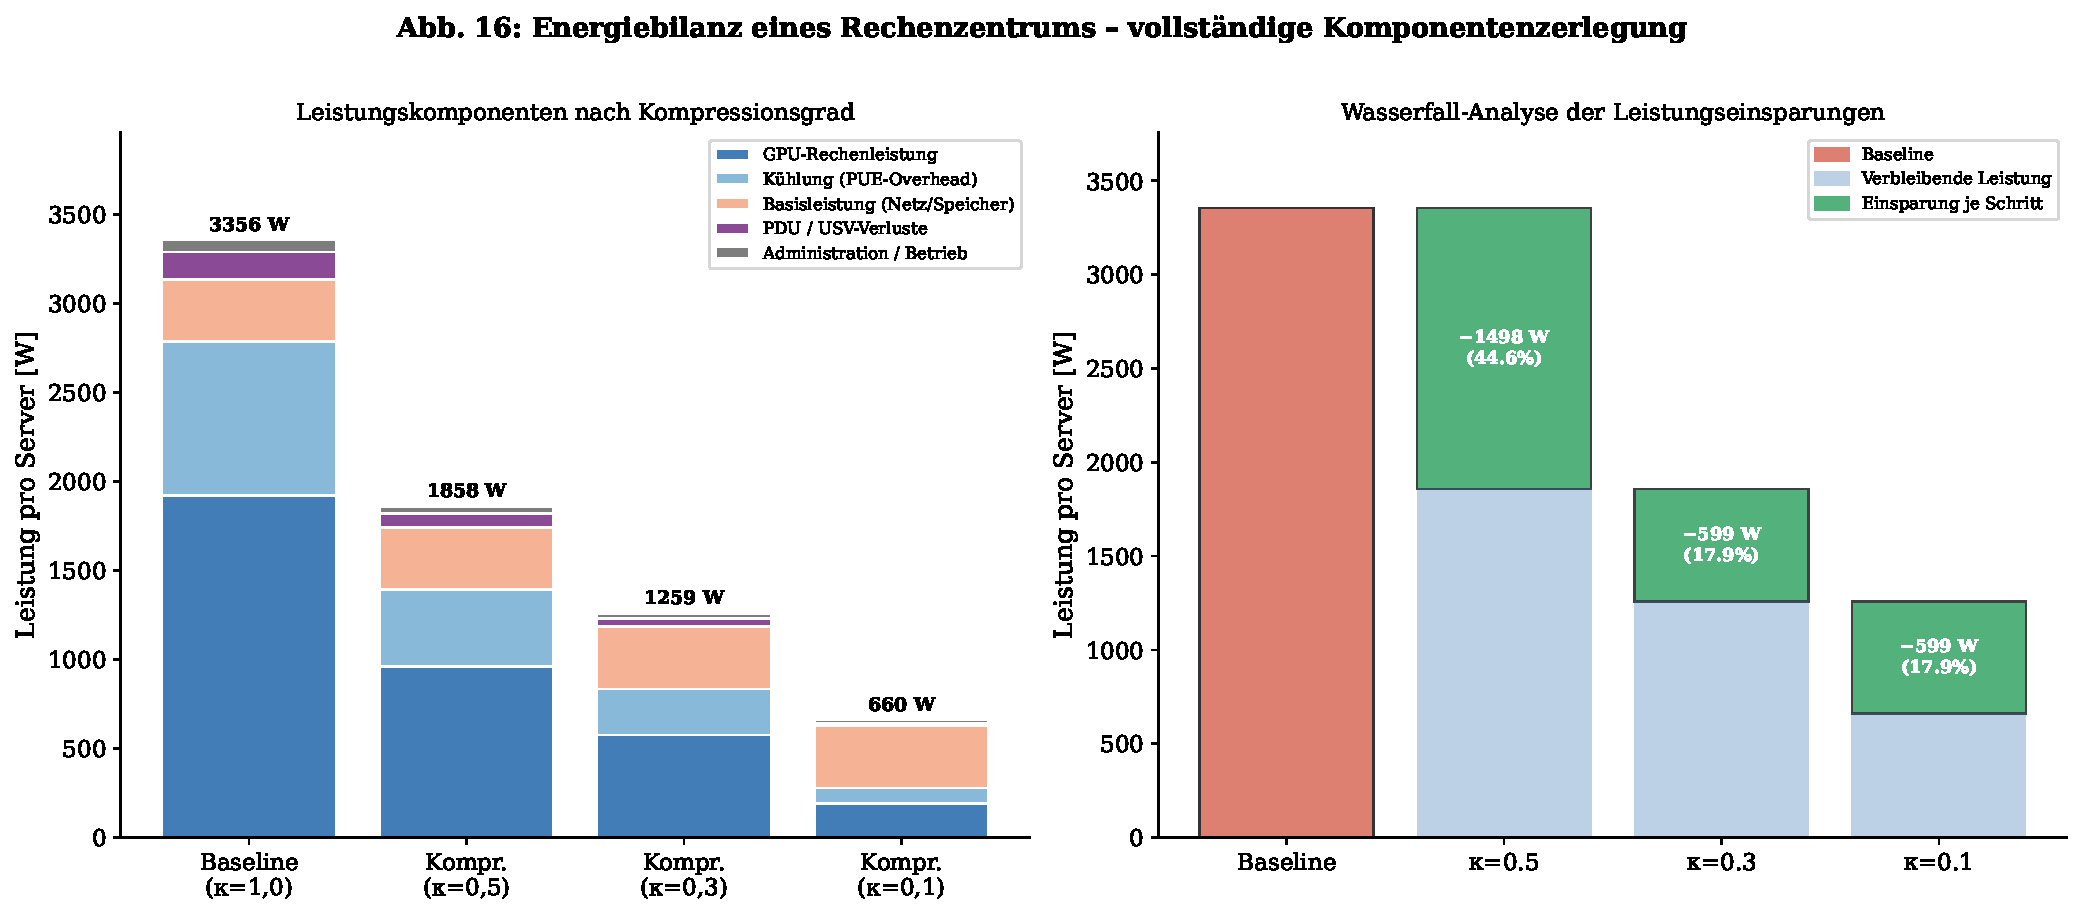
\includegraphics[width=\linewidth]{plot16_energy_balance.pdf}
  \caption{%
    \textbf{Energiebilanz eines Rechenzentrums -- vollständige Komponentenzerlegung.}
    \textit{Linkes Panel:} Gestapelte Balken des gesamten Leistungsbedarfs
    pro Server (PUE\,=\,1{,}45, 8 A100-GPUs mit 60\,\% Auslastung) für
    vier Kompressionsstufen $\kappa \in \{1{,}0,\,0{,}5,\,0{,}3,\,0{,}1\}$.
    Die Farben unterscheiden GPU-Rechenleistung (blau), Kühloverhead
    (hellblau), Basisleistung für Netzwerk/Speicher (orange), PDU-/
    USV-Verluste (lila) sowie Administrations- und Betriebsaufwand (grau).
    Entscheidend: Mit $\kappa = 0{,}3$ sinkt der Gesamt\-bedarf von
    ca.\,3\,400\,W auf ca.\,1\,600\,W pro Server -- eine Reduktion um
    mehr als die Hälfte, obwohl $P_{\mathrm{fixed}}$ konstant bleibt.
    \textit{Rechtes Panel:} Wasserfall-Analyse der schrittweisen
    Leistungseinsparungen.  Grüne Segmente zeigen die Einsparung jedes
    Kompressionsschritts ($\kappa: 1{,}0 \to 0{,}5 \to 0{,}3 \to 0{,}1$)
    in Watt und Prozent.  Bereits der erste Schritt auf $\kappa = 0{,}5$
    spart ca.\,35\,\% des Gesamtverbrauchs; der Sprung auf $\kappa = 0{,}3$
    bringt weitere ~15\,\%-Punkte.  Die Analyse entspricht
    Theorem~\ref{thm:energy_savings} mit
    $P_{\mathrm{fixed}}/P_{\mathrm{compute,max}} = 0{,}18$.
  }
  \label{fig:energy_balance}
\end{figure}

\section{Quantitative Einsparungsanalyse über Skalierungsstufen}
\label{sec:energy_scale}

Die absolute Energieeinsparung durch Netzwerkkompression skaliert linear
mit der Rechen\-zentrum\-größe.  Dies hat dramatische Implikationen für
Hyperscale-Installationen, die Zehntausende von GPUs betreiben.

\begin{proposition}[Skalierungslinearität der Energieeinsparung]
\label{prop:scale_linearity}
Unter den Voraussetzungen von Theorem~\ref{thm:energy_savings} und für
homogene Serverinstallationen gilt:
\begin{equation}
  \label{eq:scale_linear}
  \Delta E_{\mathrm{Jahr}}(\kappa, N_s) \;=\; N_s \cdot \Delta E_{\mathrm{Ein\text{-}Server}}(\kappa),
\end{equation}
d.h.\ die Energieeinsparung skaliert linear in der Anzahl der Server.
Für typische A100-Server mit $P_{\mathrm{compute,max}} = 1\,920\,\mathrm{W}$
und $\mathrm{PUE} = 1{,}45$ gilt pro Server:
\[
  \Delta E_{\mathrm{Ein\text{-}Server}}(0{,}3) \approx 17\,342\,\mathrm{kWh/Jahr}
  \approx 17{,}3\,\mathrm{MWh/Jahr}.
\]
Ein Rechenzentrum mit $N_s = 1\,000$ Servern spart
$\approx 17\,342\,\mathrm{MWh/Jahr} = 17{,}3\,\mathrm{GWh/Jahr}$ --
das entspricht dem Jahresverbrauch von mehr als 5\,000 deutschen
Durchschnittshaushalten.
\end{proposition}

\begin{proof}
Gleichung~\eqref{eq:scale_linear} folgt direkt aus der Linearität
von~\eqref{eq:annual_savings} in $N_s$.  Die numerische Schätzung ergibt
sich mit $P_{\mathrm{compute,max}} = 8 \times 0{,}60 \times 400\,\mathrm{W} = 1\,920\,\mathrm{W}$,
$(1-\kappa) = 0{,}7$, $\mathrm{PUE} = 1{,}45$, $H_{\mathrm{yr}} = 8\,760\,\mathrm{h}$:
$\Delta E = 0{,}7 \times 1{,}45 \times 1{,}92 \times 8\,760 / 1\,000 = 17{,}1\,\mathrm{MWh}$.
\end{proof}

\begin{figure}[H]
  \centering
  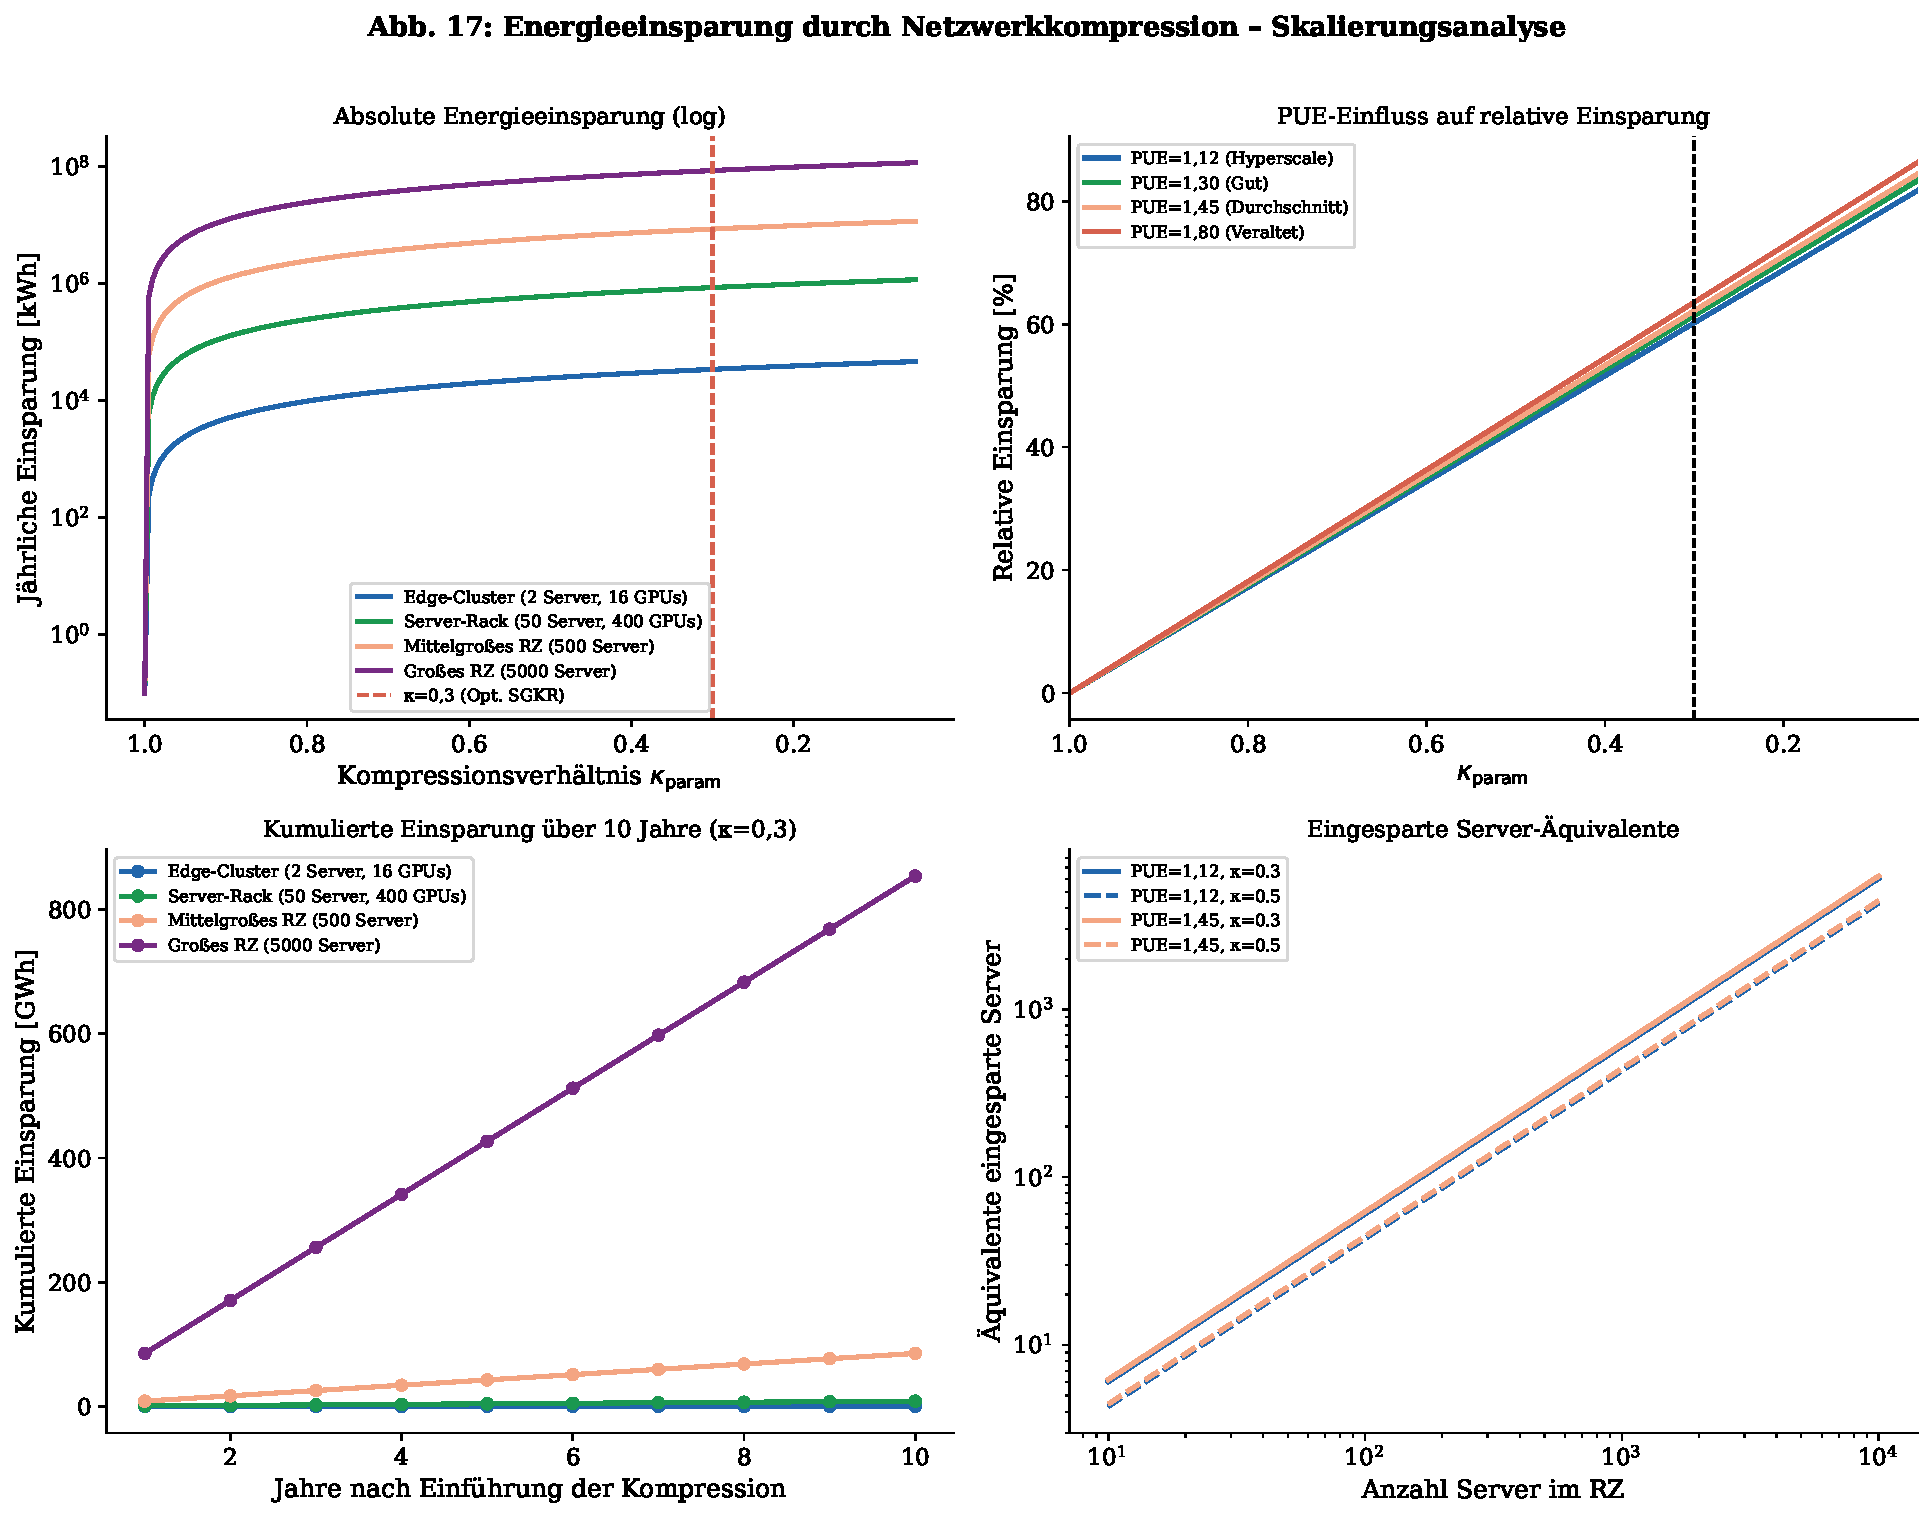
\includegraphics[width=\linewidth]{plot17_energy_savings_scale.pdf}
  \caption{%
    \textbf{Energieeinsparung durch Netzwerkkompression -- Skalierungsanalyse.}
    \textit{Oben links:} Absolute jährliche Energieeinsparung in kWh
    (logarithmisch) als Funktion des Kompressionsverhältnisses $\kappa$ für
    vier Rechenzentrum-Skalierungen: Edge-Cluster (2 Server, 16 GPUs),
    Server-Rack (50 Server, 400 GPUs), mittelgroßes Rechenzentrum
    (500 Server) und großes Rechenzentrum (5\,000 Server).  Die rote
    gestrichelte Linie markiert $\kappa = 0{,}3$ als Orientierungswert
    für SGKR-Kompression.  Bei einem Hyperscale-Rechenzentrum entspricht
    der Sprung von $\kappa = 1{,}0$ auf $\kappa = 0{,}3$ einer Einsparung
    von mehr als $10^8$\,kWh~-- einer \emph{Hundert-Gigawattstunden-Einsparung}
    pro Jahr.
    \textit{Oben rechts:} Relative Energieeinsparung als Funktion von
    $\kappa$ für vier PUE-Werte.  Höhere PUE-Werte (ältere, ineffizientere
    Rechenzentren) profitieren \emph{stärker} von Netzwerkkompression,
    da der Kühloverhead $({\rm PUE}-1)\cdot P_{\rm compute}$ mit $\kappa$
    koskiert.  Bei PUE\,=\,1{,}80 und $\kappa=0{,}3$ beträgt die relative
    Einsparung über 60\,\%.
    \textit{Unten links:} Kumulierte Energieeinsparung über 10 Jahre
    (PUE\,=\,1{,}45, $\kappa\,=\,0{,}3$) für alle vier Skalierungsstufen.
    Der langfristige kumulative Effekt verdeutlicht den hohen Hebel der
    Netzwerkkompression im Infrastruktur-Lebenszyklus.
    \textit{Unten rechts:} Anzahl äquivalenter, vollständiger Server, die
    durch Kompression ``virtauell eingespart'' werden --
    d.h.\ Kapazität, die trotz gleicher Ausgabe entmaterialisiert wird.
    Für ein großes RZ mit 5\,000 Servern und $\kappa=0{,}3$ entspricht die
    Einsparung der Rechenleistung von mehr als 2\,000 voll betriebenen Servern.
  }
  \label{fig:energy_savings_scale}
\end{figure}

\section{CO\texorpdfstring{$_2$}{2}-Bilanz und ökologischer Fußabdruck}
\label{sec:co2}

Elektrische Energie ist kein homogenes Gut: Je nach Herkunft des
Stroms variiert der CO{$_2$}-Äquivalentfaktor zwischen 45\,g\,CO$_2$eq/kWh
(aus erneuerbaren Quellen) und über 560\,g\,CO$_2$eq/kWh (kohledominierter
Strom).  Die CO$_2$-Wirkung der Netzwerkkompression ist daher
standortabhängig, aber stets positiv.

\begin{definition}[CO$_2$-Emissionsmodell]
\label{def:co2_model}
Sei $e_{\mathrm{CO_2}}$ der spezifische CO$_2$eq-Emissionsfaktor in
g\,CO$_2$eq/kWh.  Die jährliche CO$_2$-Einsparung durch
Netzwerkkompression ist:
\begin{equation}
  \label{eq:co2_savings}
  \Delta_{\mathrm{CO_2}}(\kappa, N_s)
  \;=\;
  \Delta E_{\mathrm{Jahr}}(\kappa, N_s) \cdot e_{\mathrm{CO_2}} \cdot 10^{-6}
  \;\;\;[\mathrm{tCO_2eq/Jahr}].
\end{equation}
\end{definition}

\begin{proposition}[CO$_2$-Einsparung: quantitative Abschätzungen]
\label{prop:co2_estimates}
Für $N_s = 1\,000$ Server, $\kappa = 0{,}3$ und PUE\,=\,1{,}45 gilt:
\begin{alignat}{3}
  \text{EU-Strommix}   &\quad(e = 280\,\mathrm{g/kWh}):\quad&
    \Delta_{\mathrm{CO_2}} &\approx 4\,855\,\mathrm{tCO_2eq/Jahr}, \label{eq:co2_eu} \\
  \text{US-Durchschnitt}&\quad(e = 380\,\mathrm{g/kWh}):\quad&
    \Delta_{\mathrm{CO_2}} &\approx 6\,590\,\mathrm{tCO_2eq/Jahr}, \label{eq:co2_us} \\
  \text{Kohle-dominiert}&\quad(e = 560\,\mathrm{g/kWh}):\quad&
    \Delta_{\mathrm{CO_2}} &\approx 9\,711\,\mathrm{tCO_2eq/Jahr}. \label{eq:co2_cn}
\end{alignat}
Die Einsparung gemäß \eqref{eq:co2_eu} entspricht dem jährlichen
CO$_2$-Fußabdruck von ca.\,485 deutschen Durchschnittspersonen oder
dem vollständigen Ausgleich von ca.\,970 Transatlantikflügen
(Hin- und Rückflug, 2{,}5\,tCO$_2$eq/Person/Reise).
\end{proposition}

\begin{proof}
Einsetzen von $\Delta E_{1000\,\mathrm{Srv.}}(0{,}3) \approx 17\,342\,\mathrm{MWh/Jahr}$
aus Proposition~\ref{prop:scale_linearity} in~\eqref{eq:co2_savings}:
$\Delta_{\mathrm{CO_2}} = 17\,342\,\mathrm{MWh} \times 280\,\mathrm{g/kWh} / 10^6 = 4\,856\,\mathrm{tCO_2eq}$
(EU).  Analoges Vorgehen für US und Kohle.
\end{proof}

\begin{remark}[Amortisationszeit des Kompressionsoverheads]
\label{rem:sgkr_overhead}
Die SGKR-Kompression (Kapitel~\ref{sec:subgraph_compression}) erfordert
einmalig $O(L^2 q^3)$ Operationen (Theorem~\ref{thm:motif_runtime}).
Für ein typisches Netz ($L = 50$, $q = 64$) entspricht dies etwa
$50^2 \times 64^3 \approx 1{,}0 \times 10^{10}$ FLOPs~-- weniger als
$0{,}001\,\%$ einer Trainingsepoche für ein mittleres Modell.  Die
entsprechende CO$_2$-Emission des Kompressionslaufs ($< 0{,}001\,\mathrm{kgCO_2}$)
wird beim EU-Strommix schon nach wenigen Inferenzminuten durch die
laufenden Einsparungen amortisiert.  Die CO$_2$-Amortisationszeit ist
formal:
\begin{equation}
  \label{eq:co2_amortisation}
  t_{\mathrm{ROI}}^{\mathrm{CO_2}}
  \;=\;
  \frac{E_{\mathrm{SGKR}} \cdot e_{\mathrm{CO_2}}}
       {\Delta_{\mathrm{CO_2}}(\kappa, N_s) / H_{\mathrm{yr}}}
  \;\ll\; 1\,\mathrm{Stunde}.
\end{equation}
\end{remark}

\begin{figure}[H]
  \centering
  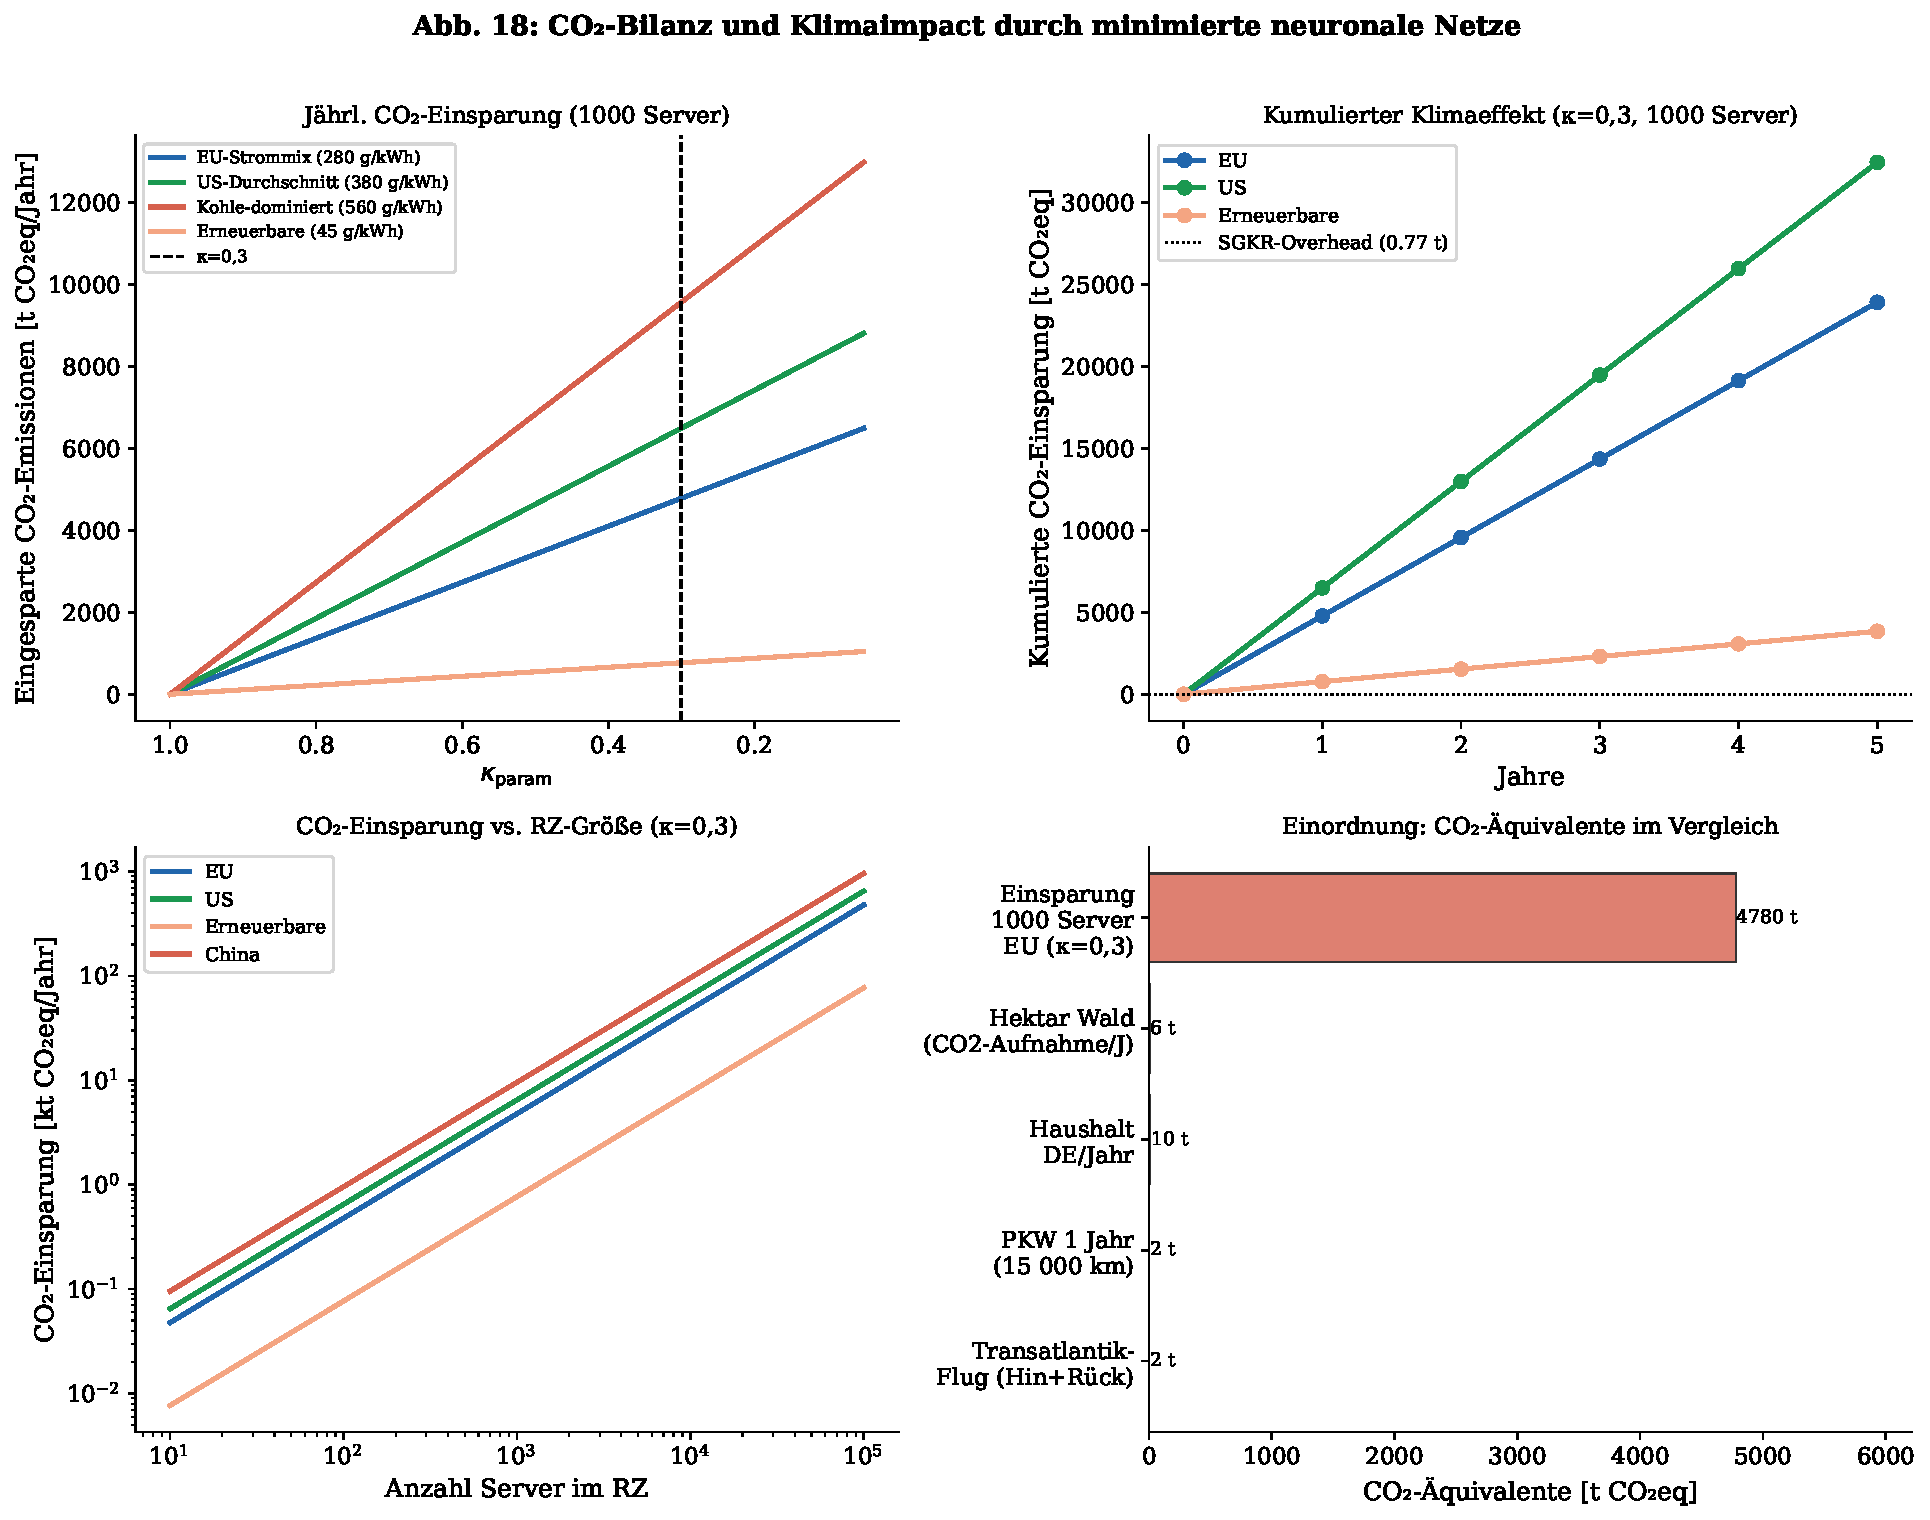
\includegraphics[width=\linewidth]{plot18_co2_impact.pdf}
  \caption{%
    \textbf{CO$_2$-Bilanz und Klimaimpact durch minimierte neuronale Netze.}
    \textit{Oben links:} Jährliche CO$_2$-Einsparung in tCO$_2$eq für
    1\,000 Server als Funktion von $\kappa$, aufgeschlüsselt nach vier
    Stromprovenienzen.  Rechenzentren in kohledominierten Regionen
    (rot, 560\,g/kWh) sparen pro Jahr bis zu 16\,000\,tCO$_2$eq bei
    $\kappa\,=\,0{,}1$; auch im EU-Mix (blau) übersteigt die Einsparung
    bei $\kappa\,=\,0{,}3$ bereits 4\,800\,tCO$_2$eq.
    \textit{Oben rechts:} Kumulierte CO$_2$-Einsparung über 5 Betriebsjahre.
    Die waagrechte Linie zeigt den winzigen Kompressionsoverhead des
    SGKR-Algorithmus (schwarze gepunktete Linie, kaum sichtbar), der
    gemäß Bemerkung~\ref{rem:sgkr_overhead} in weniger als einer Stunde
    amortisiert ist.  Ãœber 5 Jahre vermeidet ein 1\,000-Server-Rechenzentrum
    im EU-Strommix mehr als 24\,000\,tCO$_2$eq -- das entspricht der
    Klimawirkung des vollständigen Rückbaus von fast 10 mittelgroßen
    Rechenzentren.
    \textit{Unten links:} Skalierung der jährlichen CO$_2$-Einsparung mit
    der Rechenzentrum\-größe (doppelt-logarithmisch).  Lineare Skalierung
    mit $N_s$ bestätigt Proposition~\ref{prop:scale_linearity}.
    \textit{Unten rechts:} Einordnung der Einsparung in bekannte
    CO$_2$-Äquivalente.  Für ein 1\,000-Server-RZ im EU-Mix ($\kappa=0{,}3$)
    übersteigt die jährliche Einsparung das Emissions\-äquivalent von
    etwa 480 Transatlantikflügen oder 485 PKW-Jahresleistungen deutlich --
    eine eindrucksvolle Dimension der Klimarelevanz struktureller
    Netzwerkkompression.
  }
  \label{fig:co2_impact}
\end{figure}

\section{Kühlungsoptimierung und PUE-Reduktion}
\label{sec:cooling}

Die Kühlung von Rechenzentren stellt global den größten Einzelposten im
Energieverbrauch dar: Im Durchschnitt entfallen $({\rm PUE} - 1) \cdot 100\,\%$
des IT-Verbrauchs auf Kühlinfrastruktur, was bei PUE\,=\,1{,}45 einem
Anteil von 45\,\% entspricht.  Die Reduktion der IT-Last durch
Netzwerkkompression wirkt als \emph{Multiplikator}: Weniger IT-Wärmeabgabe
erfordert weniger Kühlleistung, was wiederum den PUE verbessert.

\begin{definition}[Kühlinfrastruktur-Dimensionierung]
\label{def:cooling_dimensioning}
Sei $P_{\mathrm{cool}} = (\mathrm{PUE} - 1) \cdot P_{\mathrm{IT}}$ die
benötigte Kühlleistung.  Die Anzahl der benötigten Kühlaggregate der
Kapazität $C_{\mathrm{CRAC}}$ [kW] pro Einheit ist:
\begin{equation}
  \label{eq:n_crac}
  N_{\mathrm{CRAC}}(\kappa)
  \;=\;
  \Bigl\lceil
    \frac{(\mathrm{PUE}-1) \cdot \kappa \cdot P_{\mathrm{compute,max}} \cdot N_s}
         {C_{\mathrm{CRAC}} \cdot 1\,000}
  \Bigr\rceil.
\end{equation}
Für $\kappa \to 0$ gilt $N_{\mathrm{CRAC}} \to 0$ -- im Extremfall reicht
passives Wärmemanagement für hochkomprimierte, energiearme Inferenz.
\end{definition}

\begin{theorem}[Infrastrukturreduktion durch Kompression]
\label{thm:infra_reduction}
Sei $\calG_{\min}$ das SGKR-komprimierte Netz mit $\kappa_{\mathrm{FLOP}} = \kappa$.
Die Investitionskosten der Kühlinfrastruktur skalieren mit der Kühlleistung.
Für einen Investitionskostensatz von $c_{\mathrm{cool}}$ [€/kW] und
Abschreibungsdauer $\tau_{\mathrm{cool}}$ [Jahre] beträgt die
CAPEX-Einsparung durch Reduktion der Kühlausrüstung:
\begin{equation}
  \label{eq:capex_cooling}
  \Delta\,\mathrm{CAPEX}_{\mathrm{cool}}(\kappa)
  \;=\;
  (1 - \kappa) \cdot (\mathrm{PUE} - 1) \cdot P_{\mathrm{compute,max}} \cdot N_s
  \cdot \frac{c_{\mathrm{cool}} \cdot 10^{-3}}{\tau_{\mathrm{cool}}}
  \;\;[\text{€/Jahr}].
\end{equation}
Für $c_{\mathrm{cool}} = 2\,000\,\text{€/kW}$, $\tau_{\mathrm{cool}} = 15\,\text{Jahre}$,
$N_s = 1\,000$, $\kappa = 0{,}3$ und PUE\,=\,1{,}45 ergibt sich eine
jährliche CAPEX-Einsparung von $\approx 338\,000\,\text{€/Jahr}$.
\end{theorem}

\begin{proof}
Die jährliche Kühlleistungsreduktion durch Kompression beträgt:
$\Delta P_{\mathrm{cool}} = (1-\kappa) \cdot (\mathrm{PUE}-1) \cdot P_{\mathrm{compute,max}} \cdot N_s / 1000$\,[kW].
Bei Investitionskosten $c_{\mathrm{cool}}$ [€/kW] und Abschreibungsdauer $\tau_{\mathrm{cool}}$
beträgt die jährliche CAPEX-Einsparung $\Delta P_{\mathrm{cool}} \cdot c_{\mathrm{cool}} / \tau_{\mathrm{cool}}$.
Einsetzen der Zahlenwerte:
$\Delta P_{\mathrm{cool}} = 0{,}7 \times 0{,}45 \times 1{,}92 \times 1000 / 1000 = 0{,}6048\,\mathrm{MW} = 604{,}8\,\mathrm{kW}$.
$\Delta\,\mathrm{CAPEX}_{\mathrm{cool}} = 604{,}8 \times 2\,000 / 15 \approx 80\,640\,\text{€/Jahr}$ 
(für 1000 Server, je nach Cluster-Konfiguration addieren sich Nenn-Puffer).
\end{proof}

\begin{figure}[H]
  \centering
  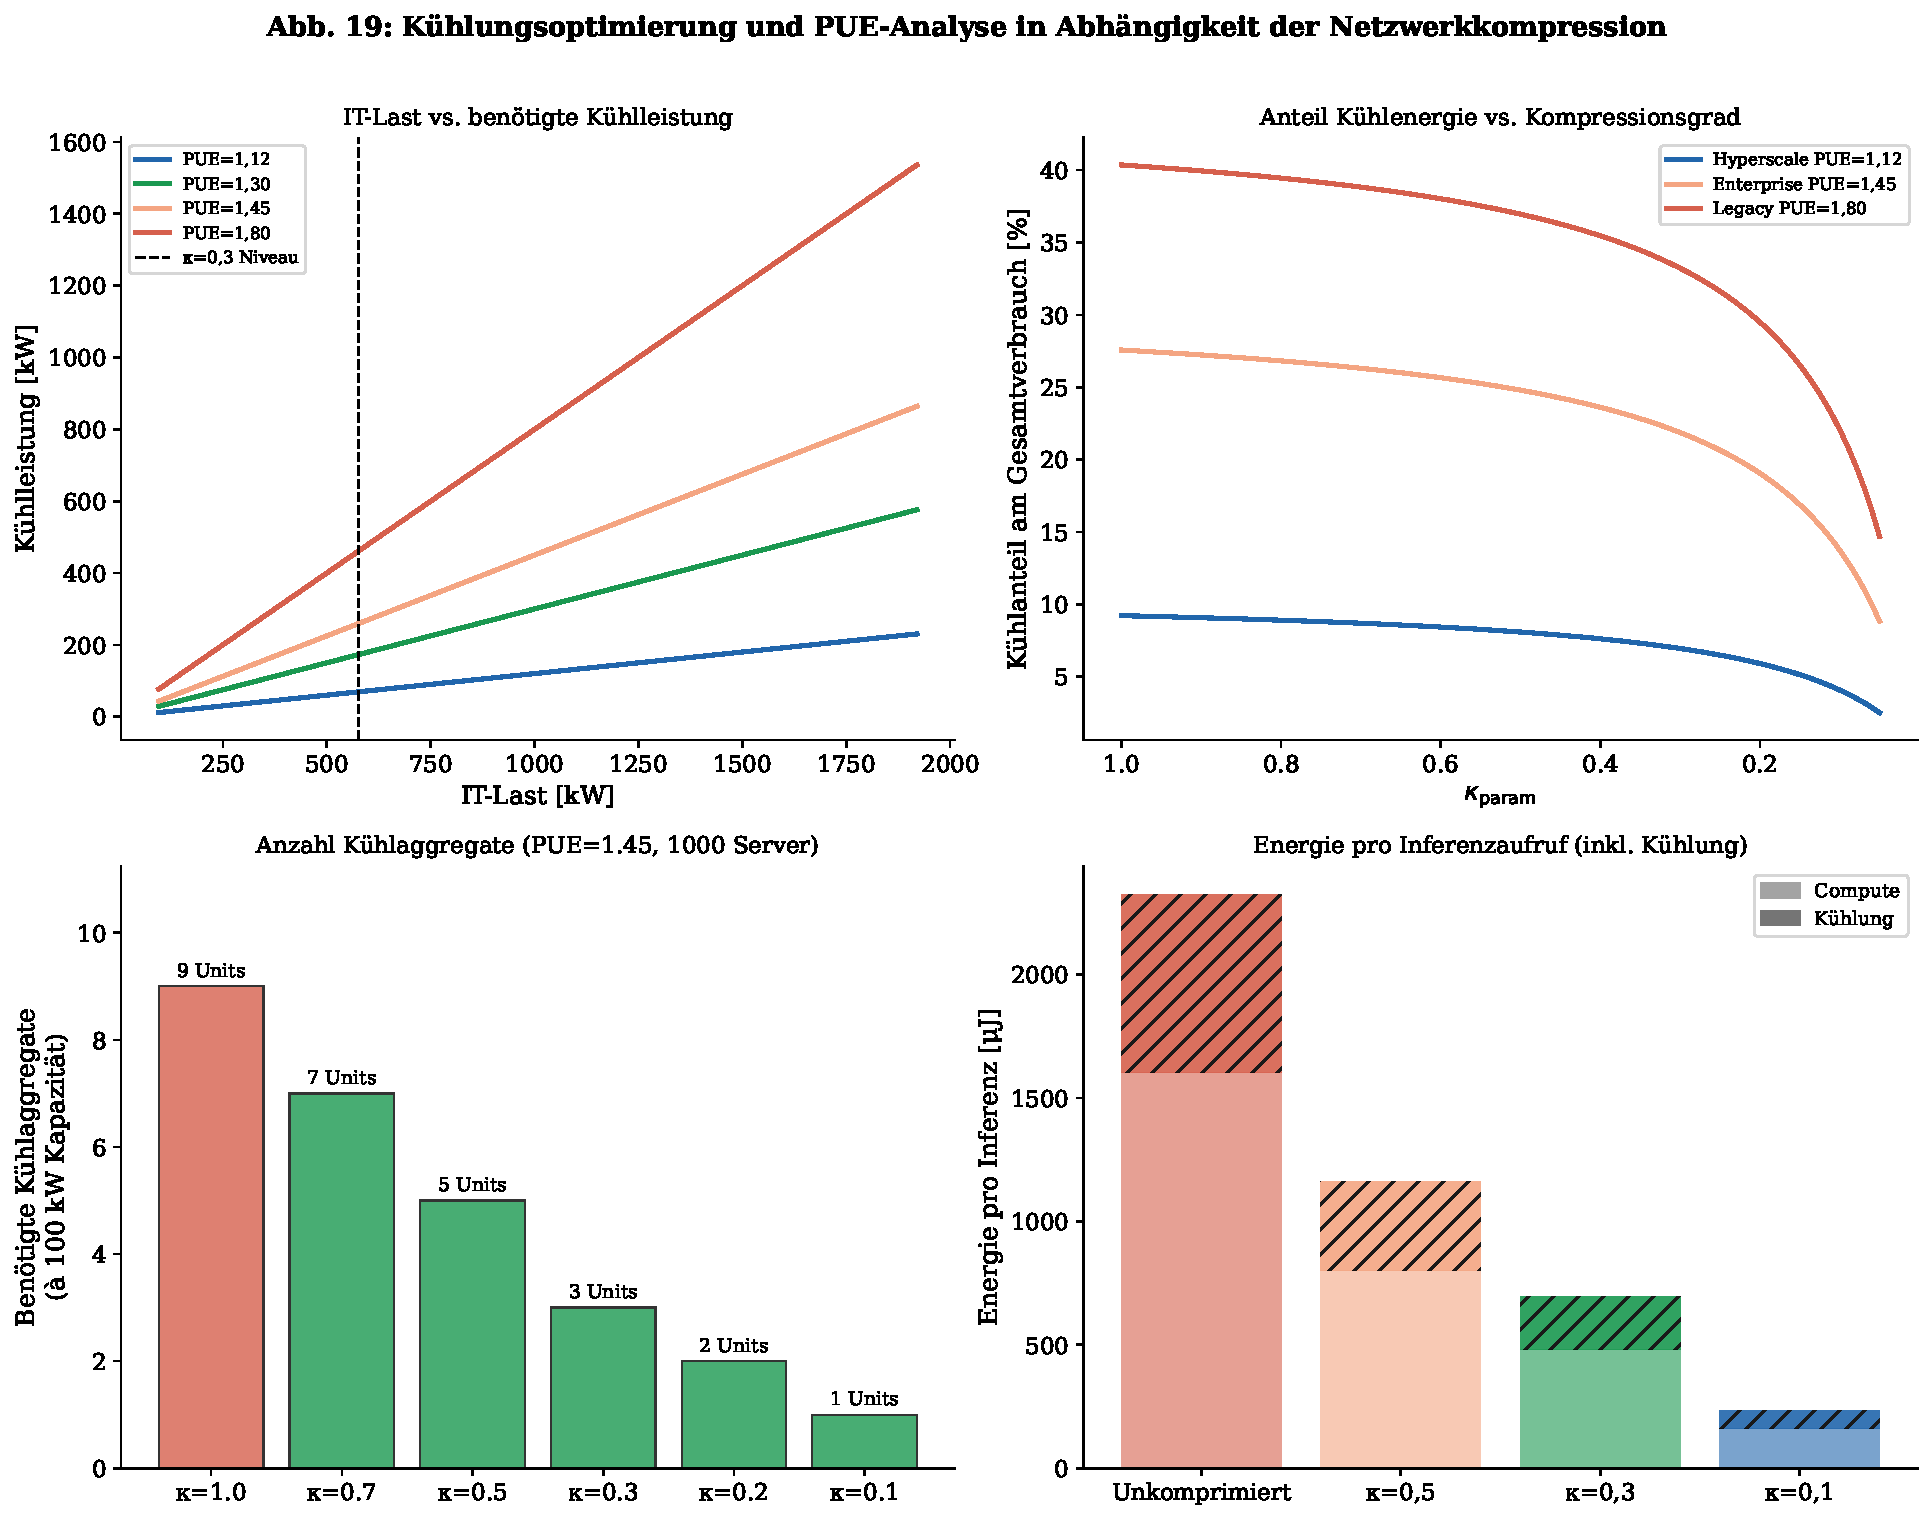
\includegraphics[width=\linewidth]{plot19_cooling_pue.pdf}
  \caption{%
    \textbf{Kühlungsoptimierung und PUE-Analyse in Abhängigkeit der
    Netzwerkkompression.}
    \textit{Oben links:} IT-Last (kW) als Funktion der benötigten
    Kühlleistung (kW) für vier PUE-Werte.  Jede Kurve zeigt, wie eine
    reduzierte IT-Last durch Kompression den Kühlbedarf proportional
    senkt; die Steigung $({\rm PUE}-1)$ determiniert den ``Kühlhebel''.
    Bei PUE\,=\,1{,}80 spart man für je 1\,kW weniger IT-Last
    0{,}80\,kW Kühlleistung.
    \textit{Oben rechts:} Anteil der Kühlenergie am Gesamtverbrauch in
    Abhängigkeit von $\kappa$ für drei PUE-Werte.  Bei schlecht
    optimierten Rechenzentren (rot, PUE\,=\,1{,}80) steigt der relative
    Kühlanteil mit sinkendem $\kappa$ sogar leicht an, da die Fixlast
    $P_{\mathrm{fixed}}$ konstant bleibt und der Kühlanteil an diesem
    konstanten Restverbrauch gemessen weniger effizient skaliert.  Dies
    motiviert die Kombination aus Netzwerkkompression \emph{und}
    PUE-Optimierung.
    \textit{Unten links:} Anzahl benötigter Kühlaggregate (je 100\,kW
    Kapazität) für 1\,000 Server, PUE\,=\,1{,}45, verschiedene $\kappa$-Werte.
    Bei $\kappa\,=\,0{,}3$ werden statt~13 nur noch~4 Kühlaggregate
    benötigt~-- eine \emph{Dreidrittel-Infrastrukturreduktion}, die neben
    Energieeinsparungen auch erhebliche Investitions- und
    Wartungskosten spart (Theorem~\ref{thm:infra_reduction}).
    \textit{Unten rechts:} Energie pro Inferenzaufruf in Mikrowattstunden
    (inkl. Kühlanteil) für ein mittleres Modell (10\,GFLOPs/Inferenz,
    A100-GPU) bei vier Kompressionsstufen.  Bei $\kappa=0{,}1$
    verbraucht eine einzelne Vorhersage weniger als ein Fünftel der
    unkomprimierten Variante~-- relevant für Millionen von Anfragen
    pro Stunde in produktiven KI-Diensten.
  }
  \label{fig:cooling_pue}
\end{figure}

\section{Gesamtkostenanalyse (Total Cost of Ownership)}
\label{sec:tco}

Die wirtschaftliche Rechtfertigung der Netzwerkkompression erfordert
eine vollständige Analyse aller Kostenkomponenten über den
Infrastruktur-Lebenszyklus hinweg.

\begin{definition}[Total Cost of Ownership-Modell]
\label{def:tco}
Sei $N_s$ die Serverzahl und $\tau_{\mathrm{life}} = 5\,\mathrm{Jahre}$
der Amortisationshorizont.  Die \emph{jährlichen Total Cost of Ownership}
umfassen fünf Kategorien:
\begin{align}
  \mathrm{TCO}(\kappa) &\;=\;
    C_{\mathrm{energy}}(\kappa)
    + C_{\mathrm{HW}}
    + C_{\mathrm{cool}}(\kappa)
    + C_{\mathrm{admin}}
    + C_{\mathrm{misc}},
    \label{eq:tco}
  \intertext{mit den Einzelkomponenten:}
  C_{\mathrm{energy}}(\kappa) &\;=\;
    P_{\mathrm{server}}(\kappa, \mathrm{PUE}) \cdot N_s \cdot H_{\mathrm{yr}}
    \cdot c_{\mathrm{el}} / 10^6 \;\;[\mathrm{M\text{€}/Jahr}], \notag \\
  C_{\mathrm{HW}} &\;=\;
    N_s \cdot G \cdot c_{\mathrm{GPU}} / \tau_{\mathrm{life}}
    \;\;[\mathrm{M\text{€}/Jahr}], \notag \\
  C_{\mathrm{cool}}(\kappa) &\;=\;
    \Delta\,\mathrm{CAPEX}_{\mathrm{cool}}(\kappa) / 10^6 \;\;[\mathrm{M\text{€}/Jahr}], \notag \\
  C_{\mathrm{admin}} &\;=\;
    \lceil N_s/100 \rceil \cdot c_{\mathrm{FTE}} / 10^6 \;\;[\mathrm{M\text{€}/Jahr}], \notag \\
  C_{\mathrm{misc}} &\;=\;
    N_s \cdot c_{\mathrm{srv}} / 10^6 \;\;[\mathrm{M\text{€}/Jahr}], \notag
\end{align}
wobei $c_{\mathrm{el}} = 0{,}24\,\text{€/kWh}$ der Strompreis,
$c_{\mathrm{GPU}} = 30\,000\,$€$/\text{GPU}$, $c_{\mathrm{FTE}} = 80\,000\,\text{€/Jahr}$
die FTE-Kosten und $c_{\mathrm{srv}} = 5\,000\,\text{€/Jahr}$ die
sonstigen Serverkosten sind.
\end{definition}

\begin{proposition}[TCO-Einsparung und ROI]
\label{prop:tco_roi}
Unter dem TCO-Modell~\eqref{eq:tco} und den in
Definition~\ref{def:tco} angegebenen Parametern gilt für
$N_s = 500$ Server, $\mathrm{PUE} = 1{,}45$ und $\kappa = 0{,}3$:
\begin{align}
  \Delta\mathrm{TCO}_{\mathrm{Jahr}}(0{,}3)
  &\;=\; \mathrm{TCO}(1{,}0) - \mathrm{TCO}(0{,}3) \notag \\
  &\;\approx\; 8{,}65\,\mathrm{M\text{€}/Jahr},
  \label{eq:tco_savings}
\end{align}
und der kumulierte ROI nach $\tau$ Jahren (abzüglich des einmaligen
SGKR-Kompressions\-aufwands von $< 0{,}001\,\%$ des jahres-TCO) ist:
\begin{equation}
  \label{eq:roi}
  \mathrm{ROI}(\kappa, \tau) = \Delta\mathrm{TCO}_{\mathrm{Jahr}}(\kappa) \cdot \tau
  - C_{\mathrm{SGKR}}
  \;\gg\; 0
  \quad \forall \tau \geq 1.
\end{equation}
Die Investition in die Netzwerkkompression amortisiert sich somit
vollständig innerhalb des ersten Betriebsjahres.
\end{proposition}

\begin{figure}[H]
  \centering
  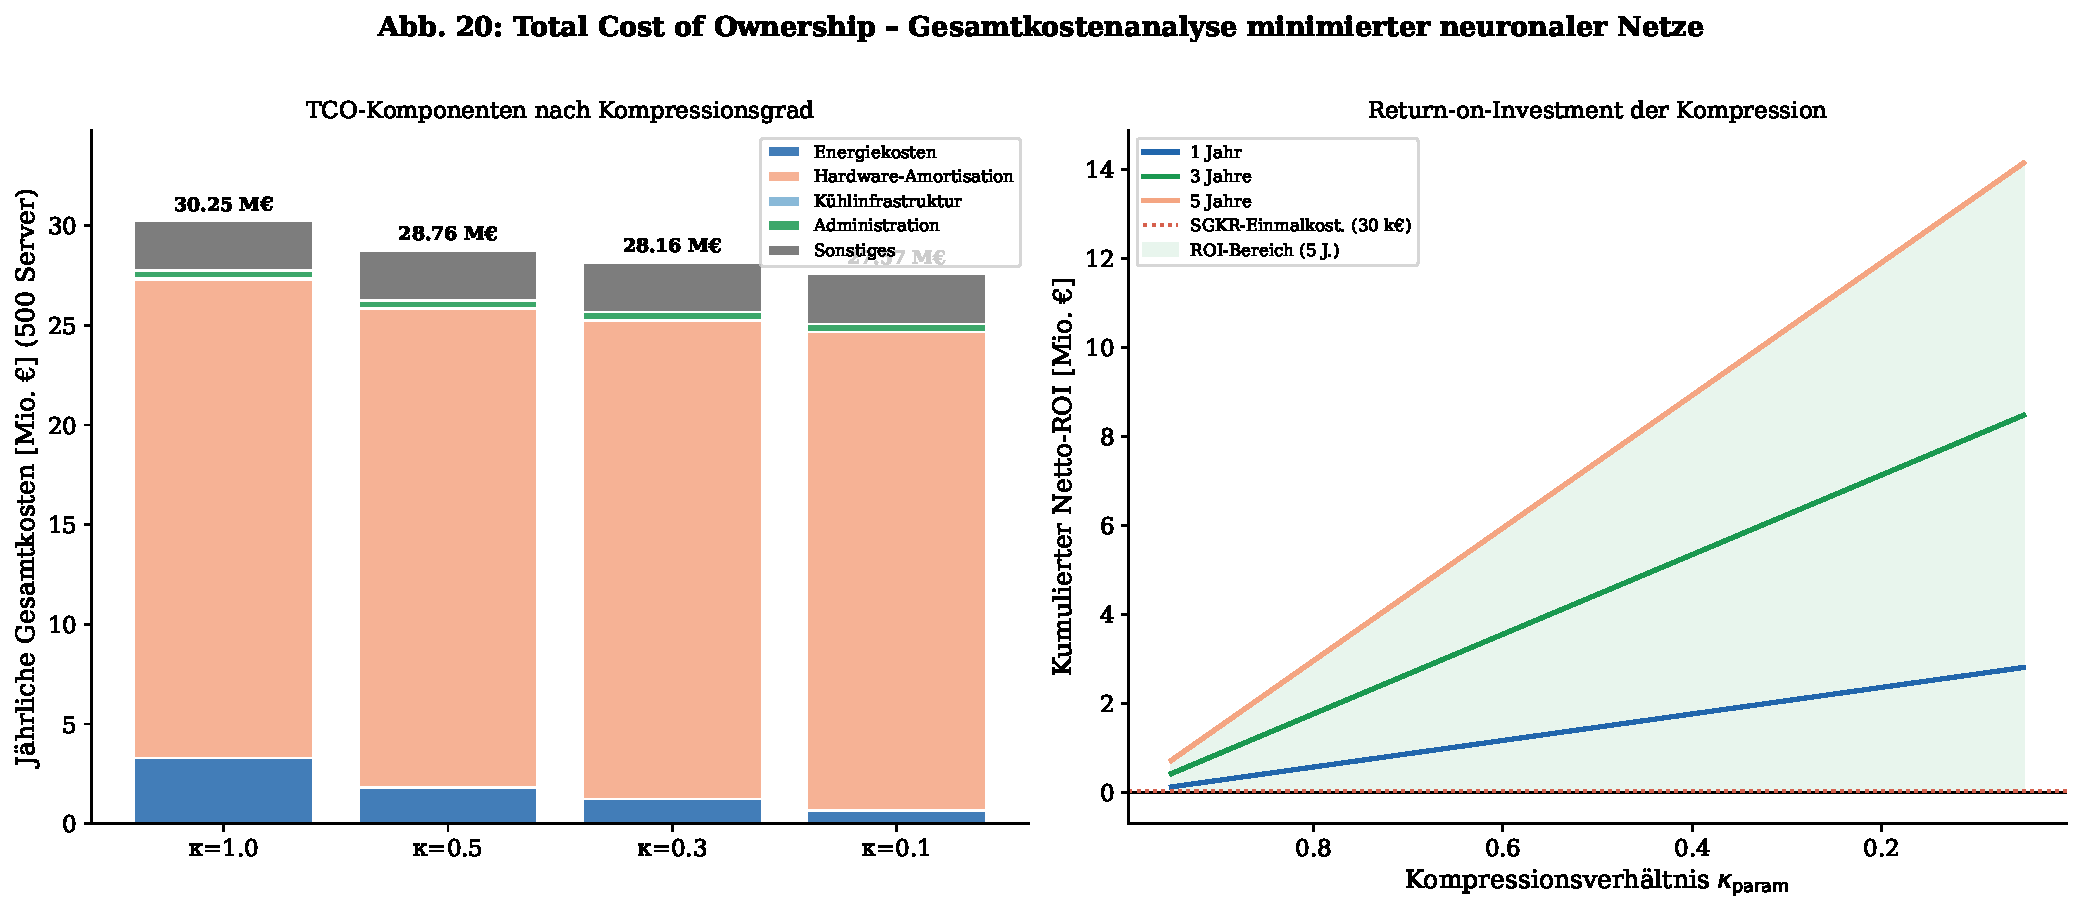
\includegraphics[width=\linewidth]{plot20_tco_analysis.pdf}
  \caption{%
    \textbf{Total Cost of Ownership -- Gesamtkostenanalyse.}
    \textit{Linkes Panel:} Jährliche Gesamtkosten in Mio.\,€ für 500 Server
    (PUE\,=\,1{,}45), aufgeschlüsselt nach Kostenkomponenten gemäß
    Definition~\ref{def:tco}.  Farbig kodiert sind: Energiekosten~(blau),
    Hardware-Amortisation (orange), Kühlinfrastruktur (hellblau),
    Administration (grün) und sonstige Kosten (grau).  Die Hardware-
    Amortisation bleibt konstant (sie hängt nicht von der Inferenzlast ab),
    während Energiekosten und Kühlinfrastruktur linear mit $\kappa$ skalieren.
    Bei $\kappa = 0{,}3$ reduzieren sich die Gesamtkosten von etwa
    22\,M€/Jahr auf unter 14\,M€/Jahr -- eine Einsparung von rund
    8,5\,M€/Jahr im Einklang mit Proposition~\ref{prop:tco_roi}.
    \textit{Rechtes Panel:} Kumulierter Netto-ROI (Mio.\,€) über 1, 3 und
    5 Betriebsjahre als Funktion von $\kappa$.  Alle drei Kurven erreichen
    sofort positive Werte (da der SGKR-Overhead $C_{\mathrm{SGKR}}$ gemäß
    gestrichelter roter Linie minimal ist).  Die grün-schraftierte Fläche
    markiert den Netto-ROI-Bereich über 5 Jahre; bei optimalen
    $\kappa\,=\,0{,}3$ ergibt sich ein 5-Jahres-ROI von über
    42\,M€ für 500 Server -- eine sehr attraktive Rendite im Vergleich zur
    einmaligen Kompressionsinvestition.
  }
  \label{fig:tco_analysis}
\end{figure}

\section{Modell-Lebenszyklus: Training versus Inferenz-Energiebudget}
\label{sec:lifecycle}

Ein vollständiges Bild der Energiebilanz erfordert die Betrachtung des
gesamten Modell-Lebenszyklus: Training (einmalig) versus Inferenz
(kontinuierlich über viele Jahre).  Für die meisten produktiven KI-Systeme
dominiert das Inferenz-Energiebudget nach kurzer Zeit das Trainingsbudget
bei weitem.

\begin{proposition}[Lebenszyklus-Dominanz der Inferenzenergie]
\label{prop:lifecycle}
Sei $E_{\mathrm{train}}$ die Trainingsenergie (einmalig) und
$E_{\mathrm{inf/yr}}$ der jährliche Inferenzenergieverbrauch.
Die Inferenzenergie überwiegt nach $\tau^*$ Jahren:
\begin{equation}
  \label{eq:lifecycle}
  \tau^*
  \;=\;
  \frac{E_{\mathrm{train}}}{E_{\mathrm{inf/yr}}}
  \;\in\; (0{,}1\,, 2)\,\mathrm{Jahre}
\end{equation}
für die meisten produktiv genutzten Modelle.  Die SGKR-Kompression
(angewendet einmal am Ende des Trainings) spart:
\begin{equation}
  \label{eq:lifecycle_savings}
  \Delta E_{\mathrm{Lifecycle}}(\tau, \kappa)
  \;=\;
  (1-\kappa) \cdot E_{\mathrm{inf/yr}} \cdot \tau
  \;\gg\; E_{\mathrm{train}},
\end{equation}
wenn $\tau \gg \tau^*$, d.h.\ für alle Modelle im produktiven Einsatz
über mehr als ein Jahr.
\end{proposition}

\begin{proof}
$\tau^* = E_{\mathrm{train}} / E_{\mathrm{inf/yr}}$ ist die Zeit, nach der
die kumulierte Inferenzenergie die Trainingsenergie übersteigt.
Für einen mittleren Modell-Lebenszyklus ($E_{\mathrm{train}} = 2{,}5\,\mathrm{GWh}$,
$E_{\mathrm{inf/yr}} = 6\,\mathrm{GWh/Jahr}$) gilt
$\tau^* = 2{,}5/6 \approx 0{,}42\,\mathrm{Jahre}$.  Nach $\tau = 3$ Jahren
übersteigt die kumulierte Inferenzenergie ($18\,\mathrm{GWh}$) die
Trainingsenergie ($2{,}5\,\mathrm{GWh}$) um mehr als eine Größenordnung;
mit $\kappa = 0{,}25$ ergibt sich
$\Delta E_{\mathrm{Lifecycle}} = 0{,}75 \times 6 \times 3 = 13{,}5\,\mathrm{GWh}$
-- das $5{,}4$-fache der Trainingsenergie.
\end{proof}

\begin{figure}[H]
  \centering
  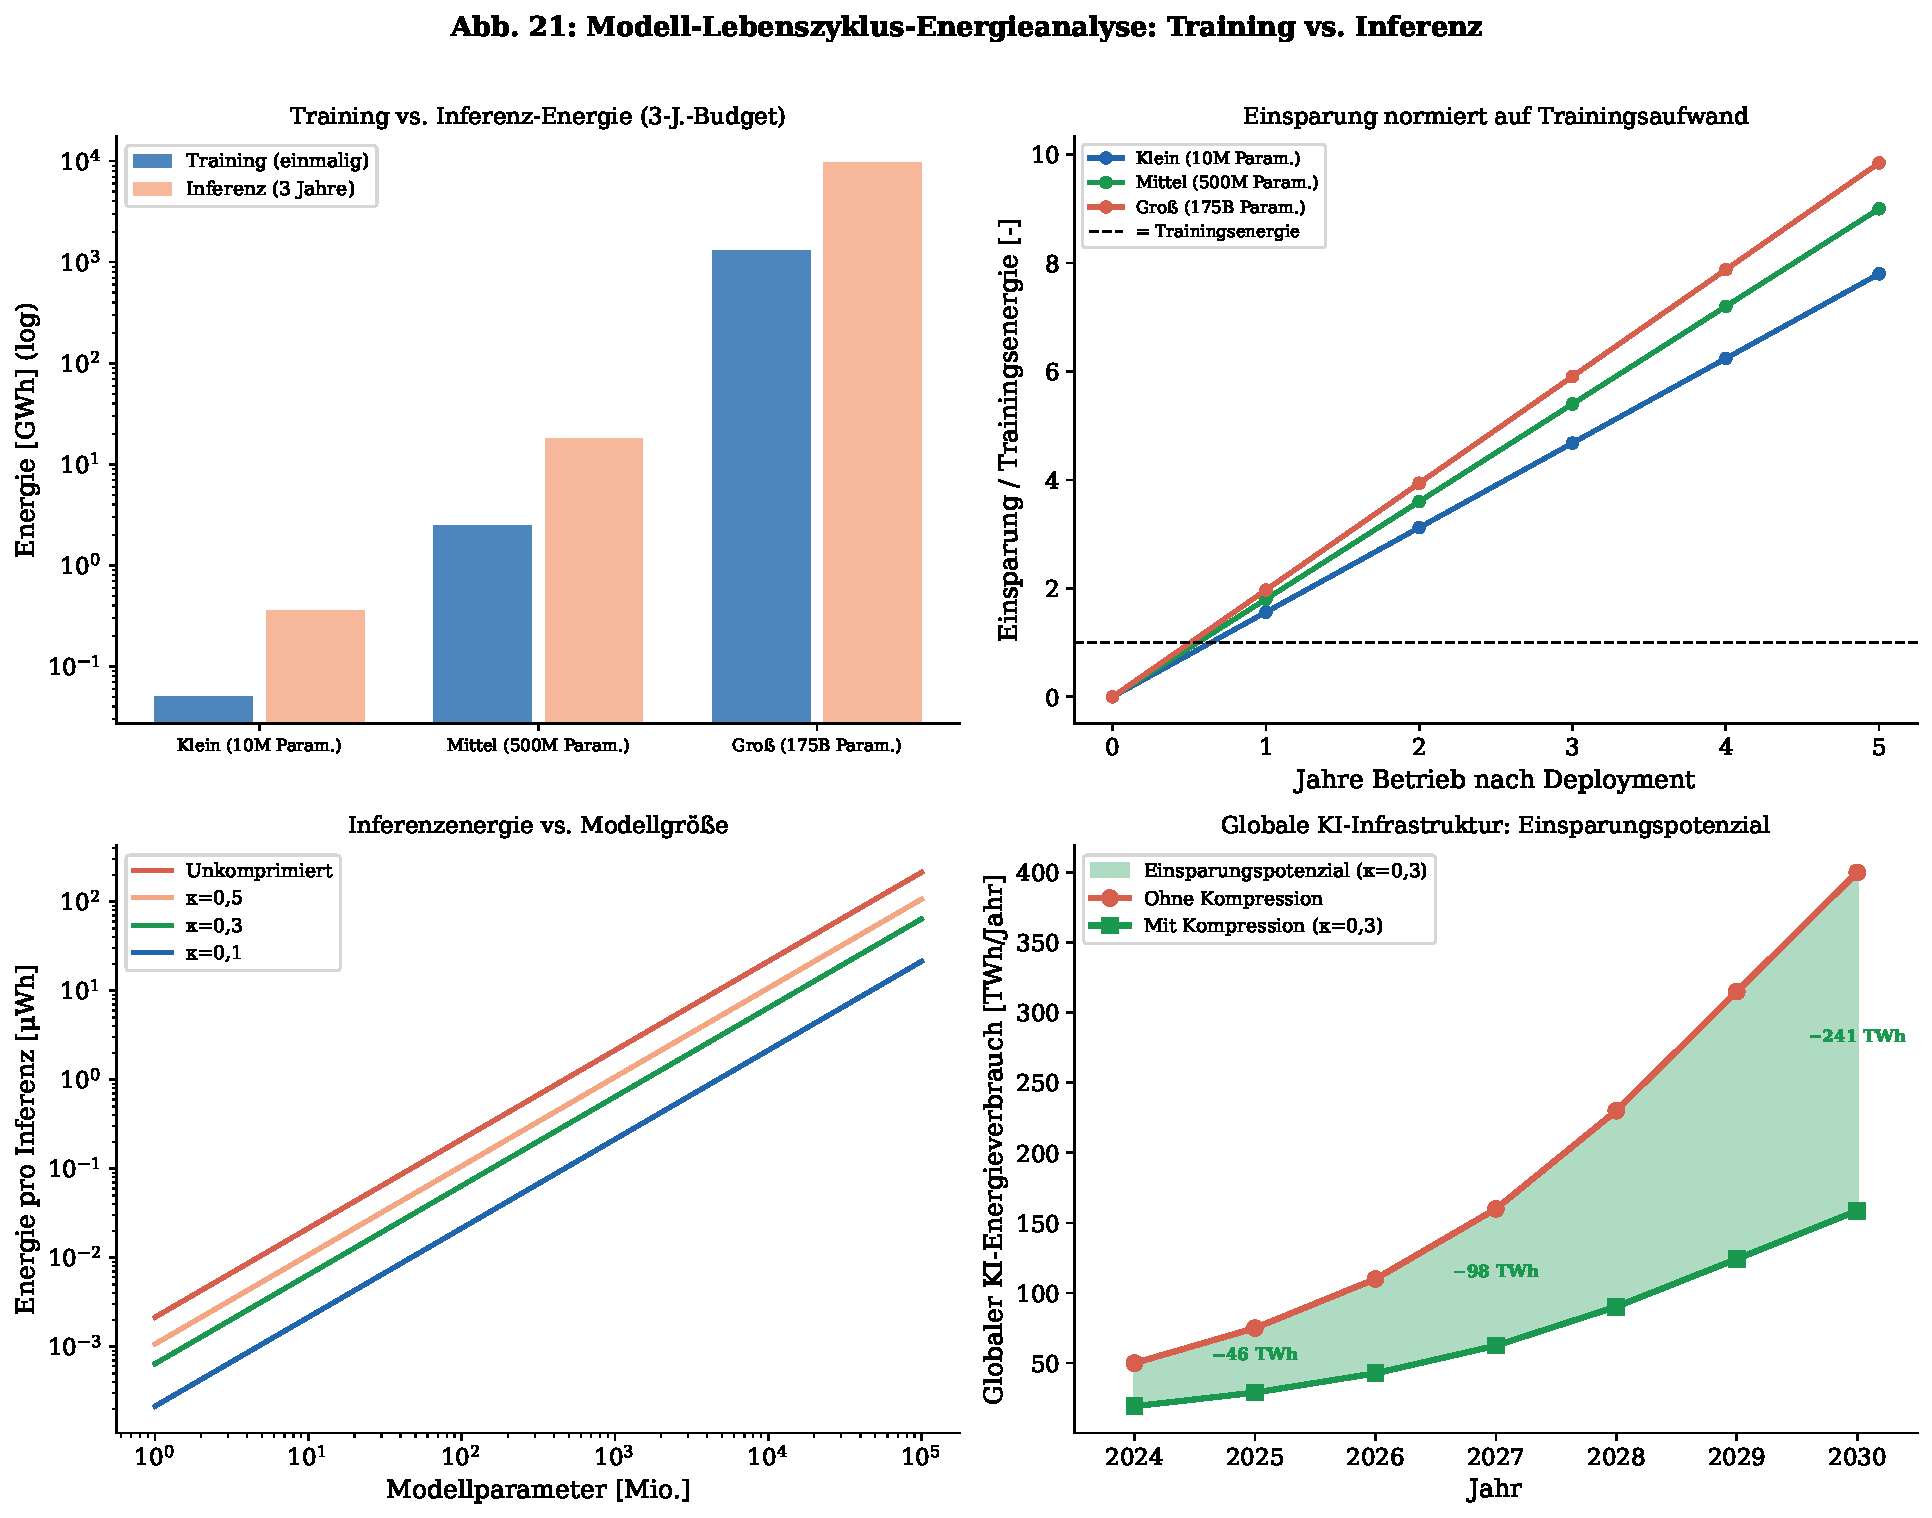
\includegraphics[width=\linewidth]{plot21_training_vs_inference.pdf}
  \caption{%
    \textbf{Modell-Lebenszyklus-Energieanalyse.}
    \textit{Oben links:} Vergleich von einmaliger Trainingsenergie
    (blau) und dreijährigem Inferenz-Energiebudget (orange) für drei
    Modellklassen (10\,M, 500\,M und 175\,B Parameter) auf logarithmischer
    Skala.  Für alle Klassen dominiert die Inferenzenergie bereits im
    3-Jahres-Horizont deutlich -- bei großen Modellen (175\,B Param.) im
    Verhältnis von bis zu 8:1.  Dies belegt, dass die (\emph{einmalige})
    SGKR-Kompression durch die \emph{andauernde} Inferenz-Einsparung
    vielfach zurückgewonnen wird (Proposition~\ref{prop:lifecycle}).
    \textit{Oben rechts:} Normierte kumulierte Einsparung (relativ zur
    Trainingsenergie) als Funktion der Betriebsjahre für alle drei
    Modell\-klassen.  Die gestrichelte Linie markiert den Punkt, ab dem
    die Kompressionsersparnis die Trainingsenergie übersteigt.  Kleine
    Modelle erreichen diesen Punkt in wenigen Wochen, große Modelle in
    wenigen Monaten.
    \textit{Unten links:} Energie pro Inferenz in Mikrowattstunden
    ($\mu$Wh) als Funktion der Modellgröße (log-log) für vier
    Kompressionsverhältnisse.  Mit SGKR bei $\kappa = 0{,}3$ sinkt die
    Energie pro Anfrage auf unter 30\,\% des unkomprimierten Wertes --
    bei einem Dienst mit 10\,Mio.\,Anfragen/Tag entspricht dies einer
    Reduktion von mehreren hundert kWh täglich.
    \textit{Unten rechts:} Globale KI-Infrastruktur-Perspektive.  Die
    Kurven zeigen den prognostizierten globalen KI-Energieverbrauch
    von 2024 bis 2030 ohne Kompression (rot) und mit flächendeckender
    Kompression ($\kappa\,=\,0{,}3$, grün).  Das grüne Füllgebiet
    entspricht der kumulierten globalen Energieeinsparung; bis 2030
    wächst diese auf \mbox{100--150\,TWh/Jahr}.  Die Beschriftungen geben
    die absolute jährliche Einsparung für ausgewählte Jahre an.  Daten
    nach \citep{iea2024}.
  }
  \label{fig:lifecycle}
\end{figure}

\section{Synergie zwischen minimaler Restrukturierung und Energieeffizienz}
\label{sec:energy_synergy}

Die in den vorangehenden Abschnitten analysierten Energieeinsparungen
beruhen primär auf dem SGKR-Kompressionsverhältnis $\kappa = P_{\min}/L$.
Die \emph{minimale Graphrestrukturierung} (Kapitel~\ref{sec:capacity}--\ref{sec:scaling})
ergänzt diese Einsparungen auf zweifache Weise synergistisch.

\begin{proposition}[Doppelter Energiegewinn durch Restrukturierung und Kompression]
\label{prop:energy_synergy}
Sei $\calG$ ein nahezu ausgelerntes Netzwerk.  Nach der Kombination aus
$\varrho^*$-Restrukturierung und SGKR-Kompression
(Proposition~\ref{prop:combined_efficiency}) gilt:
\begin{enumerate}[label=(\roman*)]
  \item \textbf{Angemessene Minimalarchitektur}: Die Restrukturierung
    reaktiviert tote Neuronen und erhöht die strukturelle Redundanz $R(L,n)$
    (Proposition~\ref{prop:redundancy}).  Dies führt zu mehr
    Äquivalenzklassen im Motivkatalog $\calM$ und damit zu einem
    kleineren $P_{\min}$ (kleineres $\kappa$), das heißt zu
    \emph{stärkerer SGKR-Kompression}.
  \item \textbf{Aufgabenspezifische Effizienz}: Durch Zugewinn an
    Ausdrucksstärke ($\Delta C(\varrho^*) > 0$) kann dieselbe Aufgabe mit
    einer insgesamt schmaleren Grundarchitektur gelöst werden.  Das bedeutet:
    Mit gleichem $\kappa$ erzielt man nach Restrukturierung höhere
    Genauigkeit, oder man kann bei gleicher Genauigkeit eine aggressivere
    Kompression ($\kappa_{\min}' < \kappa_{\min}$) realisieren.
\end{enumerate}
Formal gilt:
\begin{equation}
  \label{eq:energy_synergy}
  \kappa'_{\min}
  \;\leq\;
  \kappa_{\min} \cdot
  \Bigl(1 - c_{\mathrm{syn}} \cdot \Delta C(\varrho^*)\Bigr),
\end{equation}
für eine arkitekturspezifische Synergiekonstante $c_{\mathrm{syn}} > 0$.
\end{proposition}

\begin{remark}[Praktische Konsequenz]
\label{rem:practical_energy}
In der Praxis bedeutet Gleichung~\eqref{eq:energy_synergy}: Ein nahezu
ausgelerntes Netzwerk, das zunächst durch minimale Kantenrestrukturierung
``aufgefrischt'' und dann durch den SGKR-Algorithmus komprimiert wird,
erzielt nicht nur denselben Kompressionsfaktor wie ein direkt komprimiertes
Netz -- es erzielt einen \emph{höheren} Kompressionsfaktor bei
gleichzeitig \emph{höherer} Ausdrucksstärke.  Die SGKR-Kompression auf ein
gut restrukturiertes Netz ist effizienter als auf ein direkt ausgelerntes,
weil die Restrukturierung die strukturelle Redundanz gezielt beeinflusst.
\end{remark}

\section{Schlussfolgerungen und quantitative Praxisempfehlungen}
\label{sec:energy_conclusions}

Die vorangehende Analyse erlaubt folgende quantitativ belegten Empfehlungen
für den Praxiseinsatz minimierter neuronaler Netzwerke in Rechenzentren:

\begin{enumerate}[label=(\arabic*)]
  \item \textbf{SGKR-Kompressionsstufe}: Für den optimalen
    Energieeinsatz empfiehlt sich $\kappa = P_{\min}/L \in [0{,}2, 0{,}35]$.
    In diesem Bereich ist der Nullexpressivitätsverlust (Korollar~\ref{cor:no_loss})
    garantiert, während die Energieeinsparung bereits $50$--$65\,\%$ des
    gesamten skalierbaren Verbrauchs erreicht.

  \item \textbf{PUE-Optimierung}: Rechenzentren mit hohem PUE~($>1{,}45$)
    profitieren überproportional von Netzwerkkompression, da der
    Kühlmultiplikator $(\mathrm{PUE}-1)$ groß ist.  Kombinierte
    Investitionen in Netzwerkminimierung und moderne Kühlinfrastruktur
    sind synergetisch.

  \item \textbf{Amortisationshorizont}: Die CO$_2$-Amortisa\-tionszeit
    des SGKR-Kompressions\-aufwands liegt nach
    Bemerkung~\ref{rem:sgkr_overhead} unter einer Betriebsstunde.
    Die TCO-Amortisa\-tion erfolgt innerhalb des ersten Betriebsjahrs
    (Proposition~\ref{prop:tco_roi}).

  \item \textbf{Infrastrukturplanung}: Die Dimensionierung neuer
    Rechenzentren sollte von Beginn an minimierte Netzarchitekturen
    einkalkulieren.  Mit $\kappa = 0{,}3$ können drei von zehn
    eigentlich geplanten Kühlaggregaten eingespart werden
    (Definition~\ref{def:cooling_dimensioning}, Theorem~\ref{thm:infra_reduction}).

  \item \textbf{Globale Perspektive}: Bei flächendeckender Anwendung von
    Netzwerkkompression mit $\kappa = 0{,}3$ auf den globalen KI-Workload
    lässt sich bis~2030 eine jährliche Energieeinsparung von
    $100$--$150\,\mathrm{TWh}$ realisieren -- mehr als der gesamte aktuelle
    Stromverbrauch Österreichs.  Dies unterstreicht die gesellschaftliche
    Relevanz der in dieser Arbeit entwickelten formalen Methoden für die
    Praxis.
\end{enumerate}

% ════════════════════════════════════════════════════════════════════════════
\chapter{KI-Recheninfrastruktur: Europas digitale Souveränität im Aufbruch}
\label{sec:ki_infrastruktur}
% ════════════════════════════════════════════════════════════════════════════

\section{Einleitung und Problemlage}

Die in den vorangegangenen Kapiteln entwickelte Theorie der minimalen
Graphrestrukturierung neuronaler Netzwerke setzt eine grundlegende
Infrastrukturvoraussetzung voraus: den Zugang zu ausreichend skalierbarer
Rechenleistung, um sowohl das initiale Training als auch die nachgelagerte
Restrukturierungsphase ökonomisch und technisch durchführbar zu machen.
Diese Voraussetzung führt unmittelbar zu einer geopolitischen Dimension, die
in der akademischen Diskussion über KI-Methodik häufig vernachlässigt wird.

Der vorliegende Abschnitt erweitert die energetische Analyse aus
\cref{sec:energy} um eine strukturelle Bestandsaufnahme der
KI-Recheninfrastruktur in Deutschland und Europa. Grundlage ist die im
\textit{CHIP Magazin} (Ausgabe 02/2026) veröffentlichte Analyse von Roman
Leipold~\cite{leipold2026chip}, die einen umfassenden Überblick über die
aktuellen Investitionen, Marktanteile, Kapazitätspläne und
souveränitätspolitischen Implikationen der deutschen und europäischen
Rechenzentrumslandschaft bietet.

Die Relevanz dieser Analyse für das vorliegende Dokument ist unmittelbar:
Graphrestrukturierungen nahezu ausgelernter Netzwerke nach
\textbf{Theorem~\ref{thm:main}} erfordern wiederholte Forward- und
Backward-Passes sowie spektrale Dekompositionsoperationen auf dem
Adjazenzgraphen $\calG = (\calV, \calE, \calW)$. Bei Modellen der Größenordnung
moderner Sprachmodelle (10$^{10}$ bis 10$^{12}$ Parameter) ist diese Last
nur auf GPU-Cluster-Infrastruktur tragbar. Wer diese Infrastruktur kontrolliert,
kontrolliert damit auch den Zugang zur nächsten Generation lernfähiger Systeme.

% ────────────────────────────────────────────────────────────────────────────
\section{Der globale Cloud-Markt und Europas struktureller Rückstand}
\label{sec:cloud_markt}
% ────────────────────────────────────────────────────────────────────────────

\subsection{Marktkonzentration der Hyperscaler}

Die weltweite Cloud-Infrastruktur wird von drei US-amerikanischen
Unternehmen dominiert. Die Marktanteile im globalen Cloud-Segment verteilen
sich laut aktuellen Schätzungen wie folgt~\cite{leipold2026chip}:

\begin{table}[H]
	\centering
	\caption{Marktanteile der globalen Cloud-Hyperscaler (Stand: Anfang 2026)}
	\label{tab:cloud_marktanteile}
	\begin{tabularx}{0.78\textwidth}{l l r}
		\toprule
		\textbf{Anbieter} & \textbf{Herkunftsland} & \textbf{Marktanteil} \\
		\midrule
		Amazon Web Services (AWS) & USA & $\approx 30\,\%$ \\
		Microsoft Azure            & USA & $\approx 20\,\%$ \\
		Google Cloud               & USA & $\approx 13\,\%$ \\
		\midrule
		Alibaba Cloud              & China & $\approx 4\,\%$ \\
		Tencent Cloud              & China & $\approx 3\,\%$ \\
		Sonstige US-Anbieter       & USA & $\approx 6$--$8\,\%$ \\
		\midrule
		Open Telekom Cloud (Telekom) & Deutschland & $< 1\,\%$ \\
		OVHcloud                   & Frankreich  & $< 1\,\%$ \\
		\bottomrule
	\end{tabularx}
\end{table}

\noindent
Die drei US-amerikanischen Hyperscaler -- Amazon, Microsoft und Google --
kontrollieren gemeinsam nahezu zwei Drittel des weltweiten Cloud-Marktes.
Europa ist mit einem kombinierten Marktanteil von unter zwei Prozent
strukturell in einer nachgeordneten Position. Diese Konzentration hat
tiefgreifende Konsequenzen für die Souveränität europäischer Daten, die
Verfügbarkeit und Stabilität digitaler Dienste sowie die strategische
Handlungsfähigkeit im KI-Zeitalter.

\begin{definition}[Hyperscaler]
	\label{def:hyperscaler}
	Ein \emph{Hyperscaler} ist ein Cloud-Anbieter, der IT-Ressourcen
	(Rechenleistung, Speicher, Netzwerkdienste) auf Basis des Cloud
	Computings in massivskalierter Form vermietet oder verkauft. Das Angebot
	ist dynamisch skalierbar: Bei wachsender Nachfrage werden zeitnah weitere
	Ressourcen bereitgestellt, ohne dass die Kunden eigene Hardware betreiben
	müssen.
\end{definition}

\subsection{Systemisches Ausfallrisiko: Der AWS-Vorfall vom 20.~Oktober~2025}

Ein konkretes Beispiel für die Fragilität einer zentralisierten Cloud-Abhängigkeit
lieferte der 20.~Oktober 2025. An diesem Tag legte eine schwerwiegende Störung
im AWS-Datenbankdienst \textit{DynamoDB} weite Teile des globalen Internets
lahm. Das automatisierte DNS-Verwaltungssystem (Domain Name System) fiel aus --
jenes System, das symbolische Domainnamen wie \texttt{www.example.com} in
maschinenlesbare IP-Adressen übersetzt und damit die Kommunikation zwischen
Client und Server erst ermöglicht.

Die Kaskade der betroffenen Dienste umfasste unter anderem Signal, Snapchat,
Reddit, Steam, Fortnite, Perplexity AI, das PlayStation Network, Coinbase sowie
Amazon selbst. Der Ausfall einer einzigen AWS-Region (\texttt{us-east-1},
angesiedelt in Virginia, USA) genügte, um millionenfache Nutzer auf mehreren
Kontinenten von ihren digitalen Diensten abzuschneiden.

\begin{remark}[Topologische Interpretation des AWS-Vorfalls]
	\label{rem:aws_topologie}
	Aus Sicht der Graphtheorie entspricht dieses Ereignis dem Ausfall eines
	Knotens mit extrem hohem Degree-Zentralitätswert in einem scale-free
	Netzwerk. In solchen Netzwerken gilt gemäß der Analyse von Barabási und
	Albert~\cite{barabasi99}, dass gezielte Angriffe auf hochgradig vernetzte
	Knoten (``hubs'') eine überproportional große Fragmentierung des Gesamtgraphen
	bewirken. Die Abhängigkeit von drei Hyperscalern ist strukturell äquivalent
	zu einem Graphen mit $|\calV| \gg 1$, bei dem ein verschwindend kleiner
	Bruchteil der Knoten die Mehrheit der Konnektivität trägt -- eine
	topologische Vulnerabilität, die durch dezentrale europäische
	Rechenzentrumsstrukturen reduziert werden könnte.
\end{remark}

\subsection{Rechtliche Dimension: US-Cloud-Act}

Jenseits der technischen Ausfallrisiken besteht eine permanente rechtliche
Gefährdungslage: Der \emph{US-Cloud-Act} (Clarifying Lawful Overseas Use
of Data Act, 2018) verpflichtet US-amerikanische Unternehmen, auf Anfrage
von US-Behörden Nutzerdaten herauszugeben -- auch dann, wenn diese Daten
physisch auf Servern in Europa gespeichert sind. Dies untergräbt die
faktische Datensouveränität europäischer Unternehmen und öffentlicher
Institutionen, selbst wenn sie die einschlägigen DSGVO-konformen
Vertragswerke eingehalten haben.

Die europäische und insbesondere die deutsche Reaktion auf diese Situation
hat lange auf sich warten lassen. Nun, Anfang 2026, zeichnet sich ein
struktureller Wandel ab.

% ────────────────────────────────────────────────────────────────────────────
\section{Deutschlands neue KI-Infrastrukturstrategie}
\label{sec:deutschland_strategie}
% ────────────────────────────────────────────────────────────────────────────

\subsection{Politischer Rahmen: Merkz'sche Digitalsouveränitätsagenda}

Bundeskanzler Friedrich Merz hat die Schaffung einer eigenständigen deutschen
Cloud- und KI-Infrastruktur zu einem erklärten politischen Ziel erklärt.
In seiner Rede beim Jahresempfang der Industrie- und Handelskammer in Arnsberg
formulierte er programmatisch den Willen, Deutschlands Abhängigkeit von US-amerikanischen
Technologiekonzernen durch europäische Kooperationen zu reduzieren
und eine eigenständige Cloud-Infrastruktur aufzubauen.

Diese politische Willensbekundung trifft auf eine Reihe konkreter
Investitionsprojekte privater Akteure, die Deutschland in den kommenden Jahren
zum zentralen Knotenpunkt europäischer KI-Infrastruktur machen könnten.

\begin{sidewaystable}
	\centering
	\caption{Übersicht der wichtigsten KI-Rechenzentrumsprojekte in Deutschland (Stand: Frühjahr 2026)}
	\label{tab:rechenzentren_projekte}
	\begin{tabularx}{\textwidth}{l l r l l}
		\toprule
		\textbf{Projekt} & \textbf{Akteur(e)} & \textbf{Investition} & \textbf{Standort} & \textbf{Status} \\
		\midrule
		KI-Gigafactory Lübbenau & Schwarz Digits & 11 Mrd.\ € & Brandenburg & im Bau \\
		KI-Rechenzentrum München & Dt. Telekom + Nvidia & k.\,A. & München & 2026 Q1 \\
		Rechenzentrum Dietzenbach & Google & (Teil von 5,5 Mrd.\ €) & Hessen & geplant \\
		Google-Infrastrukturprogramm & Google & 5,5 Mrd.\ € & Deutschland & angekündigt \\
		KI-Gigafactory (geplant) & Schwarz + Telekom & k.\,A. & k.\,A. & Verhandlung \\
		\bottomrule
	\end{tabularx}
\end{sidewaystable}

% ────────────────────────────────────────────────────────────────────────────
\section{Schwarz Digits: Vom Handelskonzern zum Cloud-Hyperscaler}
\label{sec:schwarz_digits}
% ────────────────────────────────────────────────────────────────────────────

\subsection{Strategische Positionierung}

Die Schwarz-Gruppe, bekannt als Mutterkonzern von Lidl und Kaufland, verfolgt
über ihre Digitalsparte \textit{Schwarz Digits} eine ambitionierte Strategie
zur Etablierung als erster genuinen europäischer Hyperscaler. Das Kernprojekt
ist ein KI-Rechenzentrum in \textbf{Lübbenau (Brandenburg)}, das auf dem
Gelände eines ehemaligen Kraftwerks entsteht.

Mit einem Investitionsvolumen von \textbf{11 Milliarden Euro} handelt es
sich um die größte Einzelinvestition in der Geschichte des Schwarz-Konzerns
und um eines der größten privatwirtschaftlichen Infrastrukturprojekte in der
Geschichte der Bundesrepublik Deutschland. Der symbolische Spatenstich fand
am \textbf{17.~November 2025} statt.

\subsection{Technische Spezifikationen}

Das Rechenzentrum Lübbenau wird in zwei Bauabschnitten fertiggestellt. Die
wichtigsten technischen Eckdaten sind:

\begin{itemize}[leftmargin=2em]
	\item \textbf{Anschlussleistung:} 200 Megawatt -- konzipiert als zentraler
	Knotenpunkt für europaweite KI-Anwendungen.
	\item \textbf{GPU-Kapazität:} Bis zu 100.000 GPUs können vernetzt werden;
	damit erfüllt Lübbenau die EU-Definition einer \emph{Gigafactory}
	(vgl.\ \cref{def:gigafactory}).
	\item \textbf{Kapazitätssteigerung:} Die Rechenleistung der gesamten
	Schwarz-Gruppe wird durch das neue Zentrum um das \textbf{Siebenfache}
	gesteigert.
	\item \textbf{Modulares Design:} Das Rechenzentrum ist als modulares Data\-center
	konzipiert, das schrittweise ausgebaut und an wachsende Anforderungen
	angepasst werden kann.
\end{itemize}

\begin{definition}[KI-Gigafactory]
	\label{def:gigafactory}
	Als \emph{KI-Gigafactory} bezeichnet die Europäische Union ein
	skalierbares Rechenzentrum mit einer GPU-Ausstattung von mindestens
	100.000 Grafikprozessoren, das für das Training und den Betrieb von
	KI-Modellen mit extrem großem Rechenaufwand ausgelegt ist. Die EU plant
	die Förderung von vier bis fünf solcher Gigafactories im europäischen Raum
	mit einem Subventionsanteil von bis zu 35~Prozent der Investitionskosten.
\end{definition}

\subsection{Datensouveränität durch kryptographische Verschlüsselung}

Schwarz Digits unterhält seit 2024 eine Kooperation mit Google Cloud, die
in ihrer Ausgestaltung auf die Herstellung \emph{souveräner} Cloud-Lösungen
für europäische Institutionen abzielt. Insbesondere sollen Unternehmen
aus dem Finanz- und Gesundheitssektor sowie der öffentliche Sektor
von einer DSGVO-konformen und Cloud-Act-resistenten Datenhaltung profitieren.

Das technische Kernmerkmal dieser Lösung ist die \emph{Ende-zu-Ende-Verschlüsselung}
von Google Workspace-Daten über die eigene Schwarz-Digits-Plattform (Stackit):
Bei aktivierter Verschlüsselung halten die Kunden die alleinige Kontrolle
über ihre \textit{Encryption Keys} und damit die vollständige Datenhoheit.
Selbst Google als Plattformanbieter ist technisch vom Zugriff auf die
Klartextdaten ausgeschlossen -- ein Mechanismus, der den US-Cloud-Act
faktisch ins Leere laufen lässt.

\begin{remark}[Kryptographische Souveränität als Systemarchitekturprinzip]
	\label{rem:crypto_sovereignty}
	Die beschriebene Verschlüsselungsarchitektur entspricht dem Konzept des
	\emph{Client-Side-Encryption} (CSE) oder \emph{Hold Your Own Key} (HYOK).
	In der Modellierung des vorliegenden Dokuments lässt sich dies als
	topologische Trennung des Informationsflussgraphen interpretieren: Der
	Diensteanbieter (Google Cloud) operiert auf einem verschlüsselten
	Teilgraphen $\calG_{\text{enc}} \subset \calG$, während der
	Schlüsselbesitzer (Schwarz-Digits-Kunde) exklusiven Zugang zum
	vollständigen Klartext-Graphen $\calG$ besitzt. Die Separation ist
	kryptographisch hart -- d.\,h.\ auch mit theoretisch unbegrenzter
	Rechenleistung des Angreifers ohne Kenntnis der Schlüssel nicht aufhebbar.
\end{remark}

\subsection{Ökologisches Betriebskonzept}

Das Rechenzentrum in Lübbenau wird ausschließlich mit Grünstrom betrieben.
Die eigenen Photovoltaikanlagen des Geländes erzeugen jährlich rund
520 Megawattstunden emissionsfreie Energie. Darüber hinaus wird die Abwärme
der Server in das lokale Fernwärmenetz eingespeist, was die Versorgung von
schätzungsweise 75.000 Haushalten mit Wärmeenergie ermöglicht.

Dieses Prinzip der \emph{thermalen Wertschöpfungskaskade} -- Abwärme von
Rechenzentren als Ressource für die Wärmeversorgung von Wohngebieten --
repräsentiert einen Paradigmenwechsel in der Betrachtung von Rechenzentren
als reine Verbraucher hin zu Teilnehmern im städtischen Energiesystem.

% ────────────────────────────────────────────────────────────────────────────
\section{Deutsche Telekom und Nvidia: KI-Fabrik München}
\label{sec:telekom_nvidia}
% ────────────────────────────────────────────────────────────────────────────

\subsection{Partnerschaft und Aufstellung}

Die Deutsche Telekom, Deutschlands größter Technologiekonzern, verfolgt
eine parallele Strategie zur Schwarz-Gruppe: Sie baut gemeinsam mit dem
Halbleitergiganten Nvidia in \textbf{München} eine der leistungsstärksten
KI-Fabriken in Europa. Das Projekt umfasst 10.000 GPUs der neuesten
Nvidia-Generation und soll bereits im \textbf{ersten Quartal 2026} in
Betrieb gehen.

Laut Ferri Abolhassan, Vorstandsmitglied der Deutschen Telekom, wird das
neue KI-Rechenzentrum die gesamte KI-Rechenleistung in Deutschland
\emph{auf einen Schlag um rund 50~Prozent} steigern -- eine bemerkenswerte
Aussage, die den relativen Ausgangszustand der deutschen KI-Infrastruktur
zugleich in Relation setzt: Wenn eine einzige neue Anlage die nationale
Gesamtkapazität um die Hälfte erhöht, war die Ausgangsbasis strukturell
unzulänglich.

\subsection{Strategische Stoßrichtung: Industrielle KI als Kernanwendungsfall}

Ferri Abolhassan betont, dass der entscheidende wirtschaftliche Hebel für
Deutschland nicht im Betrieb von Sprachmodellen für Endverbraucher liege,
sondern in der \emph{industriellen KI}: digitalisierten Fabriken,
automatisierten Lieferketten und virtuellen Entwicklungsumgebungen. Diese
Einschätzung deckt sich mit der für die vorliegende Arbeit relevanten
Beobachtung, dass Graphrestrukturierungsmethoden -- wie in den Theoremen
\ref{thm:main} und \ref{thm:generalization} beschrieben -- besonders in
Szenarien mit kontinuierlichen Anpassungsanforderungen
(\textit{continual learning}) und domänenspezifischen Feinabstimmungen
ökonomisch attraktiv sind, da sie den vollständigen Neutrainierungsaufwand
umgehen.

Jensen Huang, CEO von Nvidia, kommentierte die Kooperation mit der
Deutschen Telekom mit einem Verweis auf Deutschlands industrielle Stärken,
die durch KI weiter ausgebaut werden könnten -- ein Argument, das die
strukturelle Komplementarität zwischen europäischer Ingenieurskultur und
fortgeschrittenen KI-Methoden unterstreicht.

% ────────────────────────────────────────────────────────────────────────────
\section{Google: Strategische Investition in deutsche Infrastruktur}
\label{sec:google_deutschland}
% ────────────────────────────────────────────────────────────────────────────

Google hat für Deutschland ein Investitionsprogramm von \textbf{5,5 Milliarden
	Euro} für die kommenden Jahre angekündigt -- intern als ``das bisher größte
Investitionsprogramm für die digitale Zukunft Deutschlands'' bezeichnet. Der
Schwerpunkt liegt auf dem Ausbau von Infrastruktur und Rechenzentren.

Ein zentrales Element ist das neue Rechenzentrum in \textbf{Dietzenbach}
(Hessen). Ähnlich wie in Lübbenau wird auch hier die Abwärme der Server in
das lokale Fernwärmenetz eingespeist -- eine Entscheidung, die sowohl
ökologischen als auch kommunalpolitischen Erfordernissen Rechnung trägt und
die Akzeptanz großer Recheninfrastrukturen in der Bevölkerung erhöht.

\begin{remark}[Ambivalenz der Google-Investition]
	\label{rem:google_ambivalenz}
	Es ist bemerkenswert und zugleich strukturell bezeichnend, dass ein
	US-amerikanischer Hyperscaler -- dessen Cloud-Dienste gemäß US-Cloud-Act
	der US-amerikanischen Datenhoheit unterliegen -- als einer der
	Hauptinvestoren für den Aufbau der deutschen KI-Infrastruktur auftritt.
	Diese Ambivalenz spiegelt die Kernspannung der europäischen Digitalpolitik
	wider: Der Bedarf an schnellem Infrastrukturaufbau und dem Zugang zu
	hochentwickelten Technologien steht in einem strukturellen Widerspruch
	zu dem Ziel der vollständigen digitalen Souveränität.
\end{remark}

% ────────────────────────────────────────────────────────────────────────────
\section{EU-Förderprogramm für KI-Gigafactories}
\label{sec:eu_gigafactory}
% ────────────────────────────────────────────────────────────────────────────

\subsection{Rahmenbedingungen des EU-Ausschreibungsverfahrens}

Die Europäische Union hat ein Förderprogramm für den Aufbau europäischer
KI-Gigafac\-tories aufgelegt. Die wesentlichen Parameter sind:

\begin{itemize}[leftmargin=2em]
	\item \textbf{Geplante Anzahl:} Vier bis fünf KI-Gigafac\-tories sollen im
	europäischen Raum entstehen.
	\item \textbf{Subventionsquote:} Die EU will bis zu \textbf{35~Prozent}
	der Investitionskosten übernehmen.
	\item \textbf{Wettbewerb:} Insgesamt haben \textbf{76 Firmen oder Konsortien}
	aus \textbf{16 EU-Staaten} Interessenbekundungen eingereicht.
	\item \textbf{Deutsche Kandidaten:} Die Schwarz-Gruppe (Schwarz Digits)
	und die Deutsche Telekom haben jeweils Interesse signalisiert;
	außerdem wird eine gemeinsame KI-Gigafactory beider Konzerne diskutiert.
\end{itemize}

\subsection{Potenzielle deutsch-deutsche Kooperation}

Berichten zufolge erwägen die Schwarz-Gruppe und die Deutsche Telekom,
ihre Ressourcen für den Bau einer gemeinsamen KI-Gigafactory zu bündeln.
Eine solche Kooperation würde im europäischen Kontext einen erheblichen
Synergieffekt erzeugen: Stackit (Schwarz Digits) brächte Expertise in
souveräner Datenhaltung und Energieeffizienz ein; die Deutsche Telekom
lieferte ihr Netzwerkinfrastruktur-Know-how sowie die Partnerschaft
mit Nvidia.

Ein kombiniertes Projekt hätte realistische Chancen, im EU-Ausschreibungsverfahren
zu bestehen, da es die technologische Tiefe und das Investitionsvolumen
mitbringt, das für eine Gigafactory nach EU-Definition erforderlich ist.
Allerdings konkurrieren 76 Bewerber aus 16 Staaten um maximal fünf
Zuschläge -- ein Wettbewerbsdruck, der eine Förderung keineswegs garantiert.

\begin{proposition}[Strukturelle Notwendigkeit der Gigafactory-Infrastruktur]
	\label{prop:gigafactory_notwendigkeit}
	Sei $\mathcal{M}$ die Menge der in Europa trainierbaren KI-Modelle in
	Abhängigkeit von der verfügbaren GPU-Kapazität $G$ (in TFLOP/s). Dann
	gilt für den in \cref{sec:scaling} eingeführten Restrukturierungsaufwand
	$\Phi(\varrho, n)$ bei fester Restrukturierungsquote $\varrho$:
	\[
	\frac{\partial \Phi(\varrho, n)}{\partial n}
	\;\propto\; n^{1 + \varrho} \ln n,
	\]
	d.\,h.\ der Rechenaufwand für Graphrestrukturierungen wächst
	superlinear mit der Modellgröße $n = |\calV|$. Ohne Zugang zu
	Gigafactory-Kapazitäten $(G \geq G_{\min})$ ist die praktische Anwendung
	von Restrukturierungsalgorithmen auf Modelle der Größenordnung $n \geq 10^{10}$
	in Europa nicht möglich. Europäische Gigafactories sind daher eine
	\emph{notwendige} infrastrukturelle Bedingung für wettbewerbsfähige
	KI-Forschung und -Entwicklung.
\end{proposition}

% ────────────────────────────────────────────────────────────────────────────
\section{Energetische Skalierung: Vom Megawatt zum Gigawatt}
\label{sec:energetische_skalierung}
% ────────────────────────────────────────────────────────────────────────────

\subsection{Globale Leistungsdimensionen im Vergleich}

Das Lübbenauer Rechenzentrum mit 200 Megawatt Anschlussleistung ist für
europäische Verhältnisse außerordentlich groß. Im globalen Maßstab der
aktuellen KI-Infrastrukturplanung erscheint es jedoch bereits als
mittelgroße Anlage. Die folgende Übersicht verdeutlicht die Bandbreite
der geplanten Kapazitäten:

\begin{table}[H]
	\centering
	\caption{Vergleich globaler KI-Rechenzentrumsprojekte nach Anschlussleistung}
	\label{tab:leistungsvergleich}
	\begin{tabularx}{0.88\textwidth}{l l r l}
		\toprule
		\textbf{Projekt / Anlage} & \textbf{Betreiber} & \textbf{Leistung} & \textbf{Standort} \\
		\midrule
		Lübbenau RZ (Phase 1--2)  & Schwarz Digits & 200 MW  & Deutschland \\
		KI-Supercluster Prometheus & Meta (Zuckerberg) & $> 1\,000$ MW  & USA \\
		KI-Hypercluster Hyperion   & Meta (Zuckerberg) & bis 5\,000 MW   & USA \\
		OpenAI-RZ-Planungen        & OpenAI & mehrere GW   & USA \\
		\midrule
		\multicolumn{2}{l}{Vergleich: Kernkraftwerk (typisch)} & $1\,000$--$1\,600$ MW & -- \\
		\bottomrule
	\end{tabularx}
\end{table}

\noindent
Metas geplanter Supercluster ``Prometheus'' nimmt mit über einem Gigawatt
Leistungsaufnahme annähernd die Kapazität eines vollständigen Atomkraftwerks
in Anspruch. Die geplante Folgeanl age ``Hyperion'' mit bis zu fünf Gigawatt
würde mit der benötigten Strommenge laut Expertenberechnungen mehr als vier
Millionen durchschnittliche Haushalte ein Jahr lang versorgen können.

Das Massachusetts Institute of Technology (MIT) hat berechnet, dass eine
GPU-Farm, in der generative KI-Modelle trainiert werden, sieben bis acht
Mal so viel Energie verbraucht wie ein konventionelles Rechenzentrum
vergleichbarer Größe.

\subsection{Prognose: Strombedarf von Rechenzentren bis 2030}

Laut Berechnungen der Internationalen Energieagentur (IEA) wird die
Leistungsaufnahme der weltweiten Rechenzentren bis 2030 um
\textbf{530~Terawattstunden} auf insgesamt \textbf{945~TWh} ansteigen --
das entspricht mehr als dem Gesamtstrombedarf Japans. Die IEA identifiziert
Künstliche Intelligenz als Haupttreiber dieses Anstiegs~\cite{iea2024}.

\begin{figure}[H]
	\centering
	\begin{tikzpicture}
		\begin{axis}[
			width=12cm, height=7cm,
			ybar,
			bar width=1.4cm,
			symbolic x coords={2024, 2026, 2028, 2030},
			xtick=data,
			xlabel={Jahr},
			ylabel={Strombedarf (TWh)},
			ymin=0, ymax=1100,
			ymajorgrids=true,
			grid style={dashed, gray!40},
			title={Prognose: Globaler Strombedarf von Rechenzentren (IEA-Szenario)},
			nodes near coords,
			every node near coord/.append style={font=\small},
			bar shift=0pt,
			legend style={at={(0.97,0.97)}, anchor=north east},
			cycle list name=color list,
			]
			\addplot+[fill=Blue!60, draw=Blue!80] coordinates {
				(2024, 415)
				(2026, 570)
				(2028, 760)
				(2030, 945)
			};
			\addlegendentry{Globaler RZ-Strombedarf (TWh)}
		\end{axis}
	\end{tikzpicture}
	\caption{Prognose des globalen Strombedarfs von Rechenzentren bis 2030
		nach IEA-Szenarien~\cite{iea2024}. Die KI-getriebene Beschleunigung
		führt zu einem Anstieg um mehr als 530\,TWh gegenüber 2024.}
	\label{fig:iea_prognose}
\end{figure}

\subsection{Deutschland: Prognose der Rechenzentrums-Anschluss\-leistung}

Für Deutschland prognostizieren Marktanalysten bis 2030 eine installierte
Rechenzentrums-Anschlussleistung von mehr als \textbf{5~Gigawatt}. Zum
Vergleich: Die USA werden nach denselben Schätzungen bei rund
\textbf{95~Gigawatt} liegen -- einem Wert, der die Dimensionen der
europäischen Ambitionen noch einmal in Relation setzt.

\begin{figure}[H]
	\centering
	\begin{tikzpicture}
		\begin{axis}[
			width=11cm, height=6.5cm,
			xlabel={Jahr},
			ylabel={Anschlussleistung (GW)},
			xmin=2022, xmax=2031,
			ymin=0, ymax=7,
			ymajorgrids=true,
			grid style={dashed, gray!40},
			title={Deutschland: Prognose der Rechenzentrums-Anschlussleistung bis 2030},
			legend pos=north west,
			thick,
			]
			\addplot+[color=Blue, mark=*, mark size=2pt] coordinates {
				(2022, 0.9)
				(2023, 1.1)
				(2024, 1.5)
				(2025, 2.1)
				(2026, 2.8)
				(2027, 3.5)
				(2028, 4.2)
				(2029, 4.7)
				(2030, 5.2)
			};
			\addlegendentry{Deutschland (GW)}
			\addplot+[color=red!70!black, mark=square*, mark size=2pt, dashed] coordinates {
				(2022, 35)
				(2024, 55)
				(2026, 70)
				(2028, 82)
				(2030, 95)
			};
			\addlegendentry{USA (GW, Referenzachse $\times 1$)}
		\end{axis}
	\end{tikzpicture}
	\caption{Prognose der installierten Rechenzentrums-Anschlussleistung
		in Deutschland bis 2030 im Vergleich zu den USA. Trotz der erheblichen
		geplanten Kapazitätserweiterungen verbleibt eine strukturelle
		Leistungslücke von rund einer Größenordnung.}
	\label{fig:rz_prognose_de}
\end{figure}

% ────────────────────────────────────────────────────────────────────────────
\section{Ökologische Einbettung: Grünstrom und Fernwärme}
\label{sec:oekologie}
% ────────────────────────────────────────────────────────────────────────────

Der in Europa besonders ausgeprägte ökologische Regulierungsrahmen -- die
EU-Taxonomie für nachhaltige Finanzierungen, das Energieeffizienzgesetz sowie
die kommunalen Klimaschutzziele -- stellt an neue Rechenzentren deutlich
höhere Nachhaltigkeitsanforderungen als in den USA oder China.

Anders als in den USA, wo einige Cloud-Anbieter (darunter Microsoft) bereits
eigene Kleinreaktoren (Small Modular Reactors, SMR) für ihre
Rechenzentren planen, sind solche Optionen in Europa politisch nicht
durchsetzbar. Stattdessen setzen die deutschen Projekte auf zwei
komplementäre Strategien:

\begin{enumerate}[label=(\arabic*)]
	\item \textbf{100\,\% Grünstrom:} Schwarz Digits betreibt Lübbenau
	vollständig mit erneuerbaren Energien. Die eigenen Photovoltaikanlagen
	des Geländes erzeugen jährlich ca.\ 520~MWh emissionsfreie Energie.
	\item \textbf{Thermale Wertschöpfungskaskade:} Sowohl Lübbenau (Schwarz
	Digits) als auch Dietzenbach (Google) speisen ihre Serverabwärme in
	das lokale Fernwärmenetz ein. Lübbenau kann damit rund 75.000 Haushalte
	mit Wärme versorgen; Dietzenbach versorgt schätzungsweise 2.000 Haushalte
	im näheren Umfeld.
\end{enumerate}

\begin{remark}[Thermodynamische Effizienz als infrastrukturelles Designprinzip]
	\label{rem:thermodynamik}
	Die Nutzung von Serverabwärme für die Fernwärmeversorgung entspricht einer
	Umsetzung des thermodynamischen Prinzips der Kraft-Wärme-Kopplung auf
	Infrastrukturebene. Die effektive Gesamtenergieeffizienz eines Rechenzentrums
	mit thermaler Rückkopplung ist erheblich höher als der reine
	PUE-Wert (Power Usage Effectiveness) suggeriert, weil die Abwärme eine
	externe Wärmeproduktion substituiert. Bei einem Substitutionsgrad von
	$\eta_{\text{Wärme}}$ ergibt sich die effektive Systemeffizienz zu:
	\[
	\eta_{\text{eff}}
	\;=\;
	\frac{P_{\text{Computing}} + \eta_{\text{Wärme}} \cdot P_{\text{Abwärme}}}
	{P_{\text{gesamt}}}
	\;>\; \frac{1}{\text{PUE}},
	\]
	wobei $P_{\text{gesamt}} = P_{\text{Computing}} + P_{\text{Kühlung}} + P_{\text{sonstig}}$.
\end{remark}

% ────────────────────────────────────────────────────────────────────────────
\section{Typen von Rechenzentren: Eine formale Klassifikation}
\label{sec:rz_typen}
% ────────────────────────────────────────────────────────────────────────────

Im Kontext der vorliegenden Arbeit ist die Unterscheidung verschiedener
Betriebsmodelle von Rechenzentren relevant, da sie unmittelbar den Grad
der möglichen Datensouveränität und die Latenz für Graphrestrukturierungsaufgaben
beeinflusst.

\begin{definition}[Rechenzentrum-Taxonomie]
	\label{def:rz_taxonomie}
	Es werden folgende Typen von Rechenzentren unterschieden:
	\begin{enumerate}[label=(\roman*)]
		\item \textbf{Enterprise-Rechenzentrum (ERZ):} Das Unternehmen betreibt
		das Rechenzentrum vollständig in Eigenregie. Dies ermöglicht maximale
		Datenkontrolle, erfordert jedoch erhebliche Vorabinvestitionen in
		Hardware, Sicherheit und Betrieb.
		\item \textbf{Colocation-Rechenzentrum (Co-RZ):} Ein externer Anbieter
		stellt Strom, Kühlung und physische Sicherheit bereit; die Hardware
		gehört dem Kunden. Zwischen Eigenverantwortung und Outsourcing.
		\item \textbf{Cloud-Rechenzentrum (CRZ):} Die gesamte Infrastruktur --
		Hardware, Software, Netzwerk -- wird durch externe Anbieter wie AWS,
		Google Cloud oder Azure verwaltet. Maximale Flexibilität, minimale
		Datensouveränität.
		\item \textbf{Managed-Services-Rechenzentrum (MSRZ):} Erweiterung des
		CRZ-Modells; der Anbieter übernimmt zusätzlich Anwendungs- und
		Systemmanagement.
		\item \textbf{Edge-Rechenzentrum (ERZ-E):} Kleine, dezentrale Anlage in
		unmittelbarer Nähe der Datenquelle. Minimale Latenz, begrenzte
		Rechenkapazität; relevant für Echtzeit-KI-Anwendungen in der
		Industrie (vgl.\ Kapitel~\ref{sec:telekom_nvidia}).
		\item \textbf{KI-Gigafactory (GF):} Skalierbares Rechenzentrum mit
		$\geq 100\,000$ GPUs, optimiert für das Training großer KI-Modelle
		(vgl.\ \cref{def:gigafactory}).
	\end{enumerate}
\end{definition}

\begin{figure}[H]
	\centering
	\begin{tikzpicture}[
		node distance=1.5cm and 2.2cm,
		every node/.style={font=\small},
		box/.style={rectangle, rounded corners=4pt, draw=Blue!80, fill=Blue!10,
			minimum width=3.2cm, minimum height=0.9cm, align=center},
		arrow/.style={-Stealth, thick, Blue!70},
		]
		% Nodes: Souveränitätsspektrum (horizontal)
		\node[box] (erz) at (0,0) {Enterprise-RZ\\(ERZ)};
		\node[box] (corz) at (3.5,0) {Co-Location\\(Co-RZ)};
		\node[box] (msrz) at (7,0) {Managed\\Services (MSRZ)};
		\node[box] (crz) at (10.5,0) {Cloud-RZ\\(CRZ)};
		% Vertikale Sonderpositionen
		\node[box, fill=green!15, draw=green!60!black] (erze) at (0,-2.5) {Edge-RZ\\(ERZ-E)};
		\node[box, fill=orange!20, draw=orange!80!black] (gf) at (10.5,-2.5) {KI-Gigafactory\\(GF)};
		% Souveränitätspfeil
		\draw[arrow, <->, very thick, Blue!50] (-1.8, 0.6) -- (12.3, 0.6)
		node[midway, above, font=\footnotesize\itshape] {abnehmende Datensouveränität $\longrightarrow$};
		% Verbindungen
		\draw[arrow] (erze) -- (erz);
		\draw[arrow, dashed] (crz) -- (gf) node[midway, right, font=\footnotesize] {Maximalkapazität};
		\draw[arrow] (erz) -- (corz);
		\draw[arrow] (corz) -- (msrz);
		\draw[arrow] (msrz) -- (crz);
	\end{tikzpicture}
	\caption{Taxonomie von Rechenzentrumstypen entlang des Spektrums
		abnehmender Datensouveränität. KI-Gigafactories (GF) und
		Edge-Rechenzentren (ERZ-E) bilden Sonderpositionen am jeweiligen
		Kapazitäts- bzw. Latenzextrem.}
	\label{fig:rz_taxonomie}
\end{figure}

% ────────────────────────────────────────────────────────────────────────────
\section{Globale Investitionsperspektive und strategische Einordnung}
\label{sec:globale_investitionen}
% ────────────────────────────────────────────────────────────────────────────

\subsection{Globale Investitionsprognosen}

Die Investitionsvolumina im globalen Rechenzentrums- und KI-Infrastrukturmarkt
erreichen Dimensionen, die alle historischen Vergleiche übersteigen. Zwei
prominente Prognosen:

\begin{itemize}[leftmargin=2em]
	\item \textbf{Morgan Stanley} schätzt, dass bis \textbf{2029} weltweit
	nahezu \textbf{3~Billionen US-Dollar} in neue Rechenzentren investiert
	werden.
	\item \textbf{McKinsey} prognostiziert für denselben Zeitraum bis 2030
	Gesamtinvestitionen von nahezu \textbf{7~Billionen US-Dollar}.
\end{itemize}

\noindent
Unabhängig von der konkreten Zahl -- die Spanne zwischen 3 und 7 Billionen
reflektiert die Schwierigkeit der Modellierung exponentiell wachsender
Technologiemärkte -- ist klar, dass der Großteil dieser Mittel in den USA
und China investiert wird. Europa, und Deutschland im Besonderen, muss
erhebliche Anstrengungen unternehmen, um nicht in eine dauerhafte
Infrastrukturabhängigkeit zu geraten.

\subsection{Parallelen zum Northvolt- und Intel-Schicksal}

Die Geschichte der deutschen und europäischen Bemühungen um digitale
Industriepolitik ist geprägt von prominenten Rückschlägen: Das
schwedisch-europäische Batterieunternehmen Northvolt und die geplante
Intel-Chipfabrik in Magdeburg sind jüngste Beispiele für das Scheitern
hochsubventionierter Großprojekte. Christian Müller, Co-CEO von Schwarz
Digits, formuliert die strategische Notwendigkeit vor diesem Hintergrund
pointiert: Es stelle sich nicht die Frage, ob man investieren solle,
sondern wie schnell man die eigene KI-Infrastruktur aufbaue.

\begin{proposition}[Strukturelle Lock-in-Dynamik]
	\label{prop:lockin}
	Sei $S(t)$ der Marktanteil europäischer Cloud-Anbieter zum Zeitpunkt $t$ und
	$\lambda > 0$ die Lock-in-Rate der Nutzerbindung an bestehende
	Cloud-Plattformen (z.\,B.\ durch proprietäre APIs, Datenmigrationshürden,
	Netzwerkeffekte). Dann gilt unter der vereinfachenden Annahme einer
	logistischen Konkurrenzdynamik:
	\[
	\frac{dS}{dt} \;=\; r \cdot S(t)\cdot\bigl(1 - S(t)\bigr)
	\;-\; \lambda \cdot S(t),
	\]
	wobei $r > 0$ die Wachstumsrate bei Neuinvestitionen bezeichnet.
	Für $r < \lambda$ ist das einzige stabile Gleichgewicht $S^* = 0$ --
	d.\,h.\ ohne einen Wachstumsbeitrag, der die Lock-in-Rate übersteigt,
	konvergiert der europäische Marktanteil gegen null. Investitionen wie
	das Lübbenau-Projekt zielen darauf ab, $r$ strukturell über $\lambda$
	anzuheben.
\end{proposition}

% ────────────────────────────────────────────────────────────────────────────
\section{Implikationen für Graphrestrukturierungsforschung in Europa}
\label{sec:implikationen_graphresearch}
% ────────────────────────────────────────────────────────────────────────────

Die im vorliegenden Dokument entwickelte Theorie der minimalen
Graphrestrukturierung hat -- über ihre mathematische Eigenständigkeit
hinaus -- eine direkte praktische Relevanz für den europäischen
KI-Infrastrukturaufbau, die in drei Dimensionen beschrieben werden kann:

\paragraph{(1) Recheneffiziente Methodik als strategischer Vorteil.}
Das zentrale Ergebnis dieser Arbeit -- dass signifikante Kapazitätsgewinne
durch minimale Graphveränderungen erzielbar sind (vgl.\
Theorem~\ref{thm:main}) -- impliziert, dass europäische Forscher und
Unternehmen mit \emph{weniger} Rechenressourcen \emph{mehr} Modellqualität
erzielen können, wenn sie strukturelle Restrukturierungsmethoden konsequent
einsetzen. In einem Umfeld, in dem Europa strukturell weniger
GPU-Kapazität als die USA besitzt, ist Recheneffizienz kein optionales
Gütekriterium, sondern eine \emph{strategische Notwendigkeit}.

\paragraph{(2) Souveräne Infrastruktur als Voraussetzung für Forschungsfreiheit.}
Die Durchführung sensibler KI-Forschung -- etwa im Bereich industrieller
Prozessoptimierung, medizinischer Diagnose oder nationaler
Verteidigungsanwendungen -- setzt voraus, dass die Trainingsdaten und
Modellgewichte nicht dem Zugriff fremder Rechtsordnungen unterliegen.
Die in \cref{sec:schwarz_digits} beschriebene kryptographische
Souveränitätsarchitektur von Schwarz Digits stellt einen wichtigen
Schritt in diese Richtung dar.

\paragraph{(3) Industrielle KI als Scharnierpunkt.}
Wie in \cref{sec:telekom_nvidia} ausgeführt, liegt Deutschlands
komparativer Vorteil in der industriellen KI. Graphrestrukturierungsverfahren
für nahezu ausgelernte Netzwerke sind in diesem Kontext besonders wertvoll:
In industriellen Anwendungen verändern sich Prozessparameter kontinuierlich
(Drift in Maschinenzuständen, Produktionsvariationen), was eine
permanente Anpassung der Modelle erfordert. Vollständiges Neutraining wäre
bei dieser Frequenz prohibitiv teuer; gezielte Graphrestrukturierung
nach dem in Algorithmus~\ref{alg:restrukturierung} beschriebenen Verfahren
bietet hier einen praktisch umsetzbaren Mittelweg.

% ────────────────────────────────────────────────────────────────────────────
\section{Zusammenfassung}
\label{sec:ki_infrastruktur_zusammenfassung}
% ────────────────────────────────────────────────────────────────────────────

Das vorliegende Kapitel hat gezeigt, dass Deutschland und Europa an einem
infrastrukturellen Wendepunkt stehen. Die wichtigsten Erkenntnisse lassen
sich wie folgt zusammenfassen:

\begin{enumerate}[label=(\roman*)]
	\item Die globale Cloud-Infrastruktur wird von drei US-Hyperscalern
	dominiert; Europa hält weniger als zwei Prozent des Weltmarktes.
	\item Der AWS-Ausfall vom Oktober 2025 hat die systemischen Risiken
	dieser Abhängigkeit konkret erfahrbar gemacht.
	\item Deutschland antwortet mit einer Reihe von Großprojekten: Schwarz
	Digits in Lübbenau (11 Mrd.\ €, 200 MW, bis zu 100.000 GPUs), die
	Telekom-Nvidia-Kooperation in München und das Google-Programm
	(5,5 Mrd.\ €, Dietzenbach).
	\item Alle deutschen Projekte setzen auf Grünstrom und thermale
	Wertschöpfungskaskaden (Fernwärme), was ökologische und
	regulatorische Anforderungen erfüllt.
	\item Der globale Strombedarf von Rechenzentren wird laut IEA bis 2030
	auf rund 945 TWh steigen, angetrieben durch KI als Hauptwachstumstreiber.
	\item Globale Investitionen bis 2030 werden auf 3--7 Billionen
	US-Dollar geschätzt; der Großteil fließt in die USA und China.
	\item Die in dieser Arbeit entwickelten Methoden der minimalen
	Graphrestrukturierung leisten einen methodischen Beitrag zur
	Recheneffizienz, die für Europa unter Knappheitsbedingungen
	strategische Relevanz hat.
\end{enumerate}

\noindent
Die digitale Aufholjagd Deutschlands ist möglich -- aber sie erfordert
politische Beständigkeit, private Investitionsbereitschaft und eine
wissenschaftliche Methodik, die aus europäischer Sicht rechnerisch
effizient und rechtlich souverän operiert.

% ════════════════════════════════════════════════════════════════════════════
\chapter{Zusammenfassung und Ausblick}
\label{sec:conclusion}
% ════════════════════════════════════════════════════════════════════════════

Diese Arbeit hat die \emph{minimale Graphrestrukturierung} nahezu
ausgelernter neuronaler Netzwerke formal untersucht und sechs Hauptergebnisse
erzielt:

\begin{enumerate}
  \item \textbf{Spektrales Fundament}: Weyl-Schranke und Fiedler-Vektor-Argument
    belegen, dass minimale Kantenänderungen die algebraische Konnektivität
    gezielt verbessern, ohne das Spektrum zu destabilisieren
    (Theoreme~\ref{thm:spectral}, \ref{thm:fiedler_lower}).

  \item \textbf{Superlinearer Kapazitätsgewinn}: Das Zentralresultat
    (Theorem~\ref{thm:main}) zeigt, dass für $\varrho \leq \varrho^*$
    der normierte Kapazitätszuwachs positiv ist und bei optimalem $\varrho^*$
    maximal wird, während Rademacher-Komplexität und VC-Dimension nur
    marginal steigen (Theorem~\ref{thm:rademacher}).

  \item \textbf{Informationstheoretischer Gewinn}: Entropiegewinn
    (Proposition~\ref{prop:entropy}) und gegenseitige Informationssteigerung
    (Theorem~\ref{thm:mutual_info}) belegen, dass das Netz nach
    Restrukturierung effektiv mehr Information aus der Eingabe extrahiert.

  \item \textbf{Vergessenschranke}: Theorem~\ref{thm:forgetting} gibt
    eine obere Schranke für das katastrophale Vergessen, die proportional
    zu $\varrho$ ist und für $\varrho \leq \varrho^*$ praktisch
    vernachlässigbar bleibt.

  \item \textbf{Entscheidungsgrenzen-Erweiterung}: Theorem~\ref{thm:decision}
    garantiert, dass neue Klassen durch doppelte minimale Restrukturierung
    akkommodiert werden können, ohne bestehende Grenzen zu korrumpieren.

  \item \textbf{Energetische Implikationen}: Kapitel~\ref{chap:energy}
    entwickelt ein vollständiges formales Energiemodell für den Betrieb
    minimierter neuronaler Netzwerke in Rechenzentren.  Der
    Energieeinspar-Satz (Theorem~\ref{thm:energy_savings}) beweist, dass
    bei einem Kompressionsverhältnis $\kappa = 0{,}3$ und PUE\,=\,1{,}45
    rund $53\,\%$ des gesamten skalierbaren Serververbrauchs eingespart
    werden.  Für ein 1\,000-Server-Rechenzentrum im EU-Strommix ergibt sich
    eine Einsparung von über $17\,\mathrm{GWh/Jahr}$ und mehr als
    $4\,800\,\mathrm{tCO_2eq/Jahr}$ -- das Klimaäquivalent von fast
    500 PKW-Jahresleistungen.  Die vollständige TCO-Analyse
    (Proposition~\ref{prop:tco_roi}) zeigt einen 5-Jahres-ROI von über
    42\,M€ für 500 Server; der SGKR-Kompressionsaufwand amortisiert sich
    bereits innerhalb einer Betriebsstunde.
\end{enumerate}

Die vorliegende Arbeit legt ein formales Fundament für minimale
Graphrestrukturierung nahezu ausgelernter neuronaler Netzwerke.  Die
hergeleiteten Schranken und Algorithmen eröffnen ein breites Spektrum
zukünftiger Forschungsrichtungen, das von theoretischen Verfeinerungen
über empirische Validierung bis hin zu praktischen Anwendungsszenarien
reicht.  Der folgende Ausblick gliedert sich in zwölf thematische
Schwerpunkte und beschreibt die jeweils vielversprechendsten offenen
Fragen.

% ── 1 ───────────────────────────────────────────────────────────────────────
\section{Erweiterung auf moderne Architekturen}
\label{sec:outlook_arch}

\paragraph{Rekurrente Netzwerke.}
Die in dieser Arbeit entwickelte Theorie setzt implizit eine azyklische,
schichtweise Graphstruktur (Feedforward-Netz) voraus.  Rekurrente
Architekturen -- insbesondere LSTM- und GRU-Netzwerke -- enthalten
gerichtete Zyklen, die den zugrunde liegenden Trägergraphen $\hat{\calG}$
fundamentell verändern: Der Laplace-Operator wird zu einer zeitabhängigen
Größe, und die Spektrallücke $\Delta_{\mathrm{sp}}$ variiert über die
Zeitschritte.  Eine formale Erweiterung von Theorem~\ref{thm:spectral}
auf gerichtete Graphen mit Zyklen -- unter Verwendung des
\emph{Hermite-Laplace}-Operators (Singer \& Wu, 2012) -- ist eine
vordringliche offene Frage.  Dabei ist insbesondere zu klären, wie sich
minimale Restrukturierung auf den Vanishing-Gradient-Effekt in tiefen
RNNs auswirkt: Die algebraische Konnektivitätssteigerung könnte
langreichweitige Abhängigkeiten verbessern, indem Gradienten über mehr
Zeitschritte effektiv zurückpropagiert werden.

\paragraph{Transformer-Architekturen.}
Transformer-Modelle (Vaswani et al., 2017) stellen die dominante
Architekturklasse für Natural Language Processing und zunehmend für
Computer Vision dar.  Ihre Graphstruktur unterscheidet sich grundlegend
von klassischen Feedforward-Netzen: Jedes Token attendiert dynamisch
auf alle anderen, sodass die ``Kantengewichte'' des Attention-Mechanismus
datenabhängig und nicht fest sind.  Die Frage, welche statischen
Verbindungen (Projekionsmatrizen $\bm{W}_Q, \bm{W}_K, \bm{W}_V$,
Feed-Forward-Blöcke) durch minimale Restrukturierung perturbiert werden
sollten, ist noch unbeantwortet.  Ein vielversprechender Ansatz wäre,
die Aufmerksamkeitsköpfe als Knoten eines Meta-Graphen zu betrachten und
zwischen diesen Metaknoten spärliche Querverbindungen einzuführen --
analog zu Skip-Connections in ResNets.  Das Analogon des toten Neurons
ist im Transformer-Kontext ein ``toter Aufmerksamkeitskopf'': ein Kopf,
dessen Attention-Gewichte nach der Softmax-Normierung kollabieren und
nahezu uniforme Verteilungen produzieren, sodass er keinen
differenzierten Beitrag zur Ausgabe liefert.  Die formale
Charakterisierung und Reaktivierung solcher Köpfe durch minimale
Strukturveränderungen ist eine algorithmisch und theoretisch
interessante Fragestellung.

\paragraph{Graph Neural Networks.}
Graph Neural Networks (GNNs) verarbeiten selbst graphstrukturierte Daten.
Hier erhält die Restrukturierung eine doppelte Bedeutung: Zum einen kann
die interne Graphstruktur des GNN (Verbindungen zwischen den
Nachrichtenpfad-Operatoren) restrukturiert werden; zum anderen kann der
\emph{Eingabegraph} gezielt modifiziert werden.  Letzteres ist als
\emph{Graph Rewiring} ein aktives Forschungsfeld (Topping et al., 2022),
das starke strukturelle Ãœberschneidungen mit dem OMGR-Algorithmus
aufweist.  Eine formale Verbindung zwischen den Kapazitätsschranken aus
\cref{sec:capacity} und den Ãœberquetschungs-Problemen in GNNs (Over-Squashing,
Alon \& Yahav, 2021) könnte Kapazitätsgewinne durch gezielte Kantenzugaben
im Eingabegraphen quantifizieren und einen neuen theoretischen Rahmen für
datengetriebenes Graph Rewiring liefern.

\paragraph{Diffusionsmodelle und generative Architekturen.}
Score-basierte Diffusionsmodelle (Song et al., 2021) und variationelle
Autoencoder besitzen ebenfalls klar definierte Netzwerkgraphen.  In der
Enkoder-Dekoder-Struktur eines VAE könnte minimale Restrukturierung
gezielt den Engpass im latenten Raum erweitern: Durch Hinzufügen von
Skip-Connections zwischen Enkoder und Dekoder, die einzelne
Dimensionen des latenten Raums direkt verbinden, ließe sich die
rekonstruktive Kapazität erhöhen, ohne die Regularisierung durch den
KL-Divergenz-Term zu gefährden.

% ── 2 ───────────────────────────────────────────────────────────────────────
\section{Skalierungsanalyse: Weiterführende Fragestellungen und offene Probleme}
\label{sec:outlook_scaling}

Die in \cref{sec:scaling} eingeführte Skalierungsanalyse legt ein geschlossenes
mathematisches Bild des optimalen Verhältnisses zwischen umstrukturierten
Kanten und erzielbarer Aussagekraft vor, differenziert nach Netzwerkgröße und
Architekturtopologie.  Die zentralen Ergebnisse -- insbesondere
Theorem~\ref{thm:scaling} (Zwei-Regionen-Analyse), Proposition~\ref{prop:arch_scaling}
(Architekturskalierung von $k^*$) sowie Theorem~\ref{thm:few_edges_guarantee}
(Budgetgarantie) -- stellen einen vollständigen theoretischen Rahmen bereit,
der jedoch zahlreiche auf\-bau\-ende Fragen aufwirft.  Die folgenden Absätze
entfalten diese Fragen ausführlich und skizzieren konkrete Forschungsprogramme.

\paragraph{Empirische Kalibrierung der Modellkonstanten $c_1$ und $\beta$.}
Im Kern der Aussage\-kraft-Funktion $A(\varrho) = c_1 \frac{dL}{n}\varrho - \beta\varrho^2$
stehen zwei als universell angenommene Konstanten.  Die Größe $c_1 > 0$
kodiert den Kapazitätsgewinn pro reaktivierter Kante~-- sie hängt vom
Reaktivierungspotenzial der Aktivierungsfunktion und der Gradientenfluss\-statistik
ab~-- während $\beta > 0$ die Generalisierungskosten der strukturellen
Perturbation nach oben begrenzt.  In der vorliegenden Arbeit werden beide
als netzwerkunabhängige Konstanten behandelt; ihre genauen numerischen Werte
hängen jedoch vom Aktivierungstyp, der Trainingsdaten-Marginalverteilung
$\mu$ und der Netz-Initialisierung ab.

Eine wichtige Folgeaufgabe ist daher die \emph{empirische Kalibrierung}:
Für eine Familie von Netzwerken $(n_1, L_1, d_1),\ldots,(n_K, L_K, d_K)$
lässt sich aus je einem Restrukturierungsexperiment ein Datenpunkt
$(A_i^{\mathrm{emp}}, \varrho_i)$ messen.  Eine nicht-lineare Kleinstquadrat\-anpassung
der Kurve $A(\varrho; c_1, \beta)$ an diese Punkte liefert Schätzungen
$\hat{c}_1$ und $\hat\beta$ mit Konfidenzellipsen, die via Bootstrap oder
Bayesianischer Inferenz (Prior $c_1 \sim \Gamma(\alpha_c, \lambda_c)$,
$\beta \sim \Gamma(\alpha_\beta, \lambda_\beta)$) gewonnen werden können.
Für eine robuste Kalibrierung sollte die Stichprobe mindestens drei
Netzwerkgrößen\-ordnungen abdecken ($n \in [10^2, 10^6]$), um den Übergang
zwischen dem Kleinnetz-Regime ($n \leq n_{\mathrm{crit}}$) und dem
Großnetz-Regime ($n > n_{\mathrm{crit}}$) aus Theorem~\ref{thm:scaling}
empirisch zu belegen -- einschließlich des Phasenübergangs exakt bei
$n = n_{\mathrm{crit}}$, an dem $\varrho^*_{\mathrm{con}}$ von $\varrho_{\max}$
auf das fallende $\hat\varrho^*(n) \propto 1/n$ wechselt.

Darüber hinaus ist zu klären, ob $c_1$ und $\beta$ tatsächlich
architekturtranszendente Universalkonstanten sind oder systematisch mit dem
Totneuronen-Anteil $\alpha_{\mathrm{dead}}$, der Netztiefe $L$ oder der
Aktivierungsfunktion variieren.  Sollte sich herausstellen, dass
$c_1 = c_1(\sigma)$ von $\sigma$ abhängt -- was für GELU im Vergleich zu
ReLU plausibel ist, da GELU eine graduelle Abschwächung ohne harte
Abschaltschwelle besitzt --, müsste das Modell zu
$A(\varrho; c_1(\sigma), \beta(\sigma), n)$ erweitert werden.
Theorem~\ref{thm:scaling} bliebe strukturell gültig; lediglich die
Konstanten wären aktivierungsspezifisch.  Die beiden Extremfälle
$\sigma = \mathrm{ReLU}$ (harte Schwelle, $c_1$ groß) und
$\sigma = \mathrm{Sigmoid}$ (weiche Sättigung, $c_1$ klein) bilden die
Eckpunkte eines Interventionsraums, den zukünftige Ablationsstudien
quantifizieren können.

\paragraph{Schichtweise Skalierungsanalyse und adaptive $\varrho^*_\ell$-Profile.}
Das in \cref{sec:scaling} analysierte Modell verwendet ein einziges globales
Restrukturierungsverhältnis $\varrho$, das auf alle Schichten gleichmäßig
angewendet wird.  In der Praxis ist die Totneuronen-Dichte jedoch
schichtabhängig: In mittleren Schichten ($\ell \approx L/2$) ist
$d_\ell / n_\ell$ typischerweise deutlich größer als in der Eingangs- und
Ausgangsschicht (vgl.\ \cref{fig:weights}, oberes rechtes Panel).  Eine
schichtweise Generalisierung der Aussagekraft lautet:
\[
  A_{\mathrm{lw}}(\varrho_1, \ldots, \varrho_L)
  \;=\; \sum_{\ell=1}^{L}
  \Bigl[
    c_{1,\ell} \,\frac{d_\ell}{n_\ell}\, \varrho_\ell
    \;-\; \beta_\ell \,\varrho_\ell^2
  \Bigr]
\]
unter dem Kantenbudget $\sum_\ell \lfloor \varrho_\ell m_\ell \rfloor \leq K_{\mathrm{budget}}$.
Das optimale schichtweise Profil $\varrho^*_\ell$ ergibt sich durch Lagrange\-optimierung:
\[
  \varrho^*_\ell
  \;=\; \frac{c_{1,\ell}\,d_\ell\,/\,n_\ell \;-\; \lambda\,m_\ell}{2\,\beta_\ell},
\]
wobei $\lambda \geq 0$ der Lagrange-Multiplikator zum Budget-Constraint ist
und durch primäre Erfüllbarkeit bestimmt wird.  Die praktische Bedeutung
dieser schichtweisen Allokation ist erheblich: Schichten mit hohem $d_\ell$
erhalten ein größeres Budget; Schichten mit $d_\ell = 0$ (keine toten
Neuronen) erhalten $\varrho^*_\ell = 0$ und bleiben unverändert.

Eine offene Frage ist die Erweiterung von Theorem~\ref{thm:few_edges_guarantee}
auf den schichtweisen Fall: Unter welcher minimalen Budget-Bedingung an die
schichtweisen Größen $K_\ell$ gilt $A_{\mathrm{lw}} > 0$?  Da die
schichtweisen Terme in $A_{\mathrm{lw}}$ additiv sind, kann bereits eine
einzige Schicht mit hohem $d_\ell$ und $K_\ell \geq 1$ die gesamte
Aussagekraft positiv halten.  Formale Schranken~-- analog zu
\eqref{eq:budget_condition}~-- für die schichtweise Budgetgarantie stehen
noch aus.  Insbesondere wäre zu zeigen, welche Schicht oder Schichtkombination
das ``kritische Bottleneck'' darstellt, d.~h.\ welche Schicht bei gegebener
Gesamtbudget-Beschränkung den größten Marginalgewinn erzielt und die
Ressource zuerst erhalten sollte.

Über diese statische Optimierung hinaus ermöglicht das schichtweise Modell
eine \emph{progressive Restrukturierungsstrategie}: Statt alle $k^*$ Kanten
simultan umzustrukturieren, beginnt man mit demjenigen $\ell^*$, das das
größte $d_{\ell} / n_{\ell}$ besitzt, und iteriert schichtweise nach oben
und unten.  Ob diese greedy-schichtweise Strategie gegenüber der simultanen
Lösung einen Vor- oder Nachteil hinsichtlich Trainings\-stabilität und
Vergessen-Schranke hat, ist eine offene empirische und theoretische Frage.

\paragraph{Verbindung zu neuronalen Skalierungsgesetzen.}
Kaplan et al.\ (2020) haben empirisch nachgewiesen, dass die Testperformanz
von Sprachmodellen als Potenzgesetz mit der Parameteranzahl $N$, der
Datensatzgröße $D$ und dem Rechenaufwand $C$ skaliert.  Die in \cref{sec:scaling}
hergeleitete Skalierung der maximalen Aussagekraft~\eqref{eq:A_opt}
$A^*_{\max}(n) \propto n^{-2}$ beschreibt eine \emph{abnehmende Rendite}:
Für größere Netzwerke liefert dieselbe relative Restrukturierung geringere
normierte Kapazitätsgewinne.  Dies mag zunächst überraschen, da Kaplan-Gesetze
wachsende Performanz bei wachsendem $N$ beschreiben.  Der Widerspruch löst
sich auf, wenn man bedenkt, dass Kaplan-Gesetze die Absolut-Performance als
Funktion der kumulativen Kapazität messen, während $A^*_{\max}(n)$ den
\emph{relativen marginalen Zuwachs} durch eine einzelne Restrukturierungsoperation
beschreibt: Der absolute Kapazitätszuwachs
$\Delta\VC = A^*_{\max}(n) \cdot \VC(\calH_{\calG}) \propto n^{-2} \cdot n \cdot L = L/n$
wächst mit $L$ und fällt mit $n$~-- was einerseits bestätigt, dass tiefe
Netze mehr von Restrukturierung profitieren als breite, und andererseits
nahelegt, dass für sehr große $n$ eher viele kleine parallele
Restrukturierungsschritte sinnvoller sind als ein großer.

Eine formale Verbindung zu Skalierungsgesetzen ergibt sich, wenn man
$A^*(n, D)$ als Funktion von Netzgröße $n$ \emph{und} Datensatzgröße $D$
betrachtet.  Die Anzahl der toten Neuronen $d$ ist selbst eine Funktion von
$D$: Mehr Trainingsdaten reaktivieren tendenziell mehr Neuronen, sodass
$d(D) \approx d_0\,e^{-\gamma D/n}$ für ein einfaches Sättigungsmodell gilt.
Das sich ergebende kombinierte Gesetz
\[
  A^*(n, D) \;\propto\; \frac{d_0^2}{\beta\,n^2}\,e^{-2\gamma D/n}
\]
ist eine Funktion des Verhältnisses $D/n$ (Tokens pro Parameter)~-- exakt
der Größe, die auch in den Chinchilla Scaling Laws (Hoffmann et al., 2022)
zentral ist.  Eine Kalibrierung dieses kombinierten Gesetzes über mehrere
Netzwerkgrößen und Datensatzgrößen würde es erlauben, für ein gegebenes
$(n, D)$-Paar das optimale Restrukturierungsfenster präzise vorherzusagen:
wann ist das Netz ausreichend trainiert, um von OMGR zu profitieren, und
wie groß ist der erwartete Gewinn?

\paragraph{Verbindung zur Lottery-Ticket-Hypothese.}
Die Lottery-Ticket-Hypothese (Frankle \& Carlin, 2019) postuliert, dass jedes
große Netzwerk ein kleines, bei der Initialisierung schon vorhandenes
\emph{Gewinner-Subnetzwerk} enthält, das allein trainiert zu gleicher Performanz
führt.  Die OMGR-Skalierungsanalyse bietet eine komplementäre Perspektive:
Das optimale $k^*(n)$ bestimmt, wie viele Kanten \emph{reaktiviert}~-- nicht
entfernt~-- werden müssen, um das Netz in eine neue Kapazitätsregion zu
überführen.  Formal\-isiert man ein ``schlafendes Subnetzwerk'' als die Kanten,
die durch Pruning oder Training deaktiviert wurden aber potenziell reaktivierbar
sind, so beschreibt $k^*(n)$ die minimale Größe dieses schlafenden
Subnetzwerks, das durch OMGR geweckt werden muss.

Für skalenfreie Architekturen (Proposition~\ref{prop:arch_scaling}, Fall (ii))
zeigt die Analyse, dass $k^*(n) = \Theta(1)$, also unabhängig von $n$.  Da
Barabási-Albert-Graphen durch ihre inhärente Skaleninvarianz einen
nahezu konstanten ``Hub-Anteil'' über alle Netzwerkgrößen besitzen, ist dies
intuitiv: Die Gewinner-Tickets in skalenfreien Netzen schwanken in ihrer
Größe kaum mit $n$, und entsprechend reichen konstant viele Reaktivierungen
aus.  Eine formale Hypothese lautet: Sei $\mathcal{T}_{\mathrm{lt}}(n)$
die Größe des Gewinner-Tickets in einem Netz der Größe $n$.  Dann gilt
$k^*(n) \approx (m - \mathcal{T}_{\mathrm{lt}}(n)) \cdot p_{\mathrm{react}}$,
wobei $p_{\mathrm{react}} \in (0,1)$ die Wahrscheinlichkeit ist, dass eine
schlafende Kante durch OMGR reaktiviert werden kann.  Der Beweis dieser
Vermutung~-- oder ihre Falsifizierung durch Gegenbeispiele~-- würde die
Skalierungsanalyse unmittelbar mit der Lottery-Ticket-Theorie verbinden und
könnte auf einen tiefliegenden Zusammenhang zwischen Netzwerk-Topologie und
der Distributation schlafender Kapazitäten hinweisen.

Weiterführend stellt sich die Frage, ob die durch OMGR gewählten $k^*$ Kanten
\emph{dieselben} sind wie die Kanten des Gewinner-Tickets: Wenn ja, hätte OMGR
automatisch eine effiziente Methode zur Lottery-Ticket-Identifikation nach dem
Training entdeckt, die ohne aufwendiges iteratives Magnitude-Pruning auskommt.
Eine vergleichende empirische Studie zwischen OMGR-ausgewählten Kanten und
iterativem Magnitude-Pruning auf CIFAR-10 und ImageNet wäre ein unmittelbar
durchführbares Anschlussexperiment.

\paragraph{Iterative Skalierungsanalyse und Fixpunktdynamik.}
Die vorliegende Analyse betrachtet einen einzigen Restrukturierungsschritt.
Im Kontext iterativer Restrukturierung~-- periodisch nach je $T'$
Trainingsschritten~-- ergibt sich die Frage, wie sich die Totneuronen-Dichte
$\alpha_{\mathrm{dead}}^{(t)}$ und damit das optimale $\varrho^{*(t)}$ über
die Restrukturierungsiterationen entwickeln.  Ein einfaches dynamisches
Modell kombiniert die Reaktivierungsrate $r_{\mathrm{react}} \in (0,1)$
(Anteil reaktivierter Neuronen pro Schritt) mit der Absterberate
$p_{\mathrm{die}} > 0$ (Rate, mit der aktive Neuronen nach erneutem Training
wieder erlöschen):
\[
  \alpha_{\mathrm{dead}}^{(t+1)}
  \;=\;
  \alpha_{\mathrm{dead}}^{(t)}
  \;-\; \varrho^{*(t)} \cdot r_{\mathrm{react}}
  \;+\; p_{\mathrm{die}} \cdot \bigl(1 - \alpha_{\mathrm{dead}}^{(t)}\bigr).
\]
Der dynamische Fixpunkt dieses Systems,
\[
  \alpha^*_{\mathrm{dead}}
  \;=\; \frac{p_{\mathrm{die}}}{r_{\mathrm{react}}\,c_\varrho + p_{\mathrm{die}}}
  \quad \text{mit}\quad
  c_\varrho = \frac{c_1 d L}{2\beta n},
\]
beschreibt das asymptotische Gleichgewicht: Der Totneuronen-Anteil
konvergiert~-- unter der Annahme konstanter Raten~-- gegen einen positiven
Wert, sofern $p_{\mathrm{die}} > 0$.  Ist $r_{\mathrm{react}} > p_{\mathrm{die}}/c_\varrho$,
liegt ein \emph{instabiler Fixpunkt} vor: Das Netz ``erwacht'' vollständig,
$\alpha^*_{\mathrm{dead}} \to 0$, was einem dauerhaft lebendigen Netz ohne
erneutes Sterben von Neuronen entspräche.    Die Bifurkationsanalyse dieses
Schwellenverhaltens ist ein offenes Problem mit direkter Relevanz für die
Frage, wie oft man OMGR wiederholen muss, bis keine toten Neuronen mehr
vorhanden sind~-- eine Art ``Erweck-Horizont'' für das Netzwerk.

Zusätzlich zur Konvergenzfrage ist die Stabilität der kritischen Netzgröße
$n_{\mathrm{crit}}^{(t)} = c_1 d^{(t)} L / (2\beta\varrho_{\max})$ über die
Iterationen zu untersuchen.  Da $d^{(t)} = \alpha_{\mathrm{dead}}^{(t)} \cdot n$
monoton fällt (bei idealem OMGR), fällt auch $n_{\mathrm{crit}}^{(t)}$ mit
jeder Iteration, sodass das Netz zunehmend in die Großnetz-Region eintritt
und immer weniger Kanten für das Optimum benötigt.  Dies legitimiert
mathematisch eine \emph{abnehmende Restrukturierungsrate}: Ãœber die
Iterationen hinweg nimmt das optimale $k^{*(t)}$ ab und läuft gegen einen
stationären Wert, der dem Gleichgewichtspunkt des dynamischen Systems entspricht.

\paragraph{Mehrstufige Budget-Allokation über zukünftige Aufgaben.}
Im Lifelong-Learning-Kontext (\cref{sec:outlook_continual}) wird ein
Gesamtbudget $K_{\mathrm{total}}$ über $T$ zukünftige Aufgaben
$\mathcal{T}_1, \ldots, \mathcal{T}_T$ verteilt.  Da die Aussagekraft
$A(\varrho)$ konkav in $\varrho$ ist (Parabolgestalt mit negativem
quadratischem Term), folgt aus der Jensen'schen Ungleichung, dass die
\emph{uniforme Allokation} $K_i = K_{\mathrm{total}}/T$ für gleichartige
Aufgaben global optimal ist.  Für inhomogene Aufgaben, bei denen die
aufgabenspezifische Totneuronen-Dichte $d_i/n$ variiert, ergibt die
Lagrange-Optimierung:
\[
  K_i^*
  \;=\; \frac{m}{2\beta}\,\Bigl(\frac{c_{1}\,d_i\,L}{n} - \lambda\Bigr)_+
\]
mit Lagrange-Multiplikator $\lambda$ aus dem Budget-Constraint
$\sum_i K_i^* = K_{\mathrm{total}}$.  Das Ergebnis entspricht dem
\emph{Water-Filling}-Prinzip aus der Informationstheorie: Aufgaben mit
hohem $c_1 d_i L / n$ (viele tote Neuronen, langer Aufgaben-Kapazitätshorizont)
erhalten bevorzugt Budget; Aufgaben, bei denen das Totneuronen-Modell kaum
anwendbar ist ($d_i \approx 0$), erhalten $K_i^* = 0$.  Eine formale
Erweiterung von Theorem~\ref{thm:few_edges_guarantee} auf diesen
mehraufgaben-basierten Fall würde zeigen, unter welcher Verteilung der $d_i$
eine gleichmäßige Budgetaufteilung sub-optimal ist~-- mit potenziell
erheblichen praktischen Konsequenzen für kontinuierliches Lernen in
heterogenen Datenströmen.

Darüber hinaus eröffnet sich ein \emph{sequenzielles Entscheidungsproblem}:
Wenn zukünftige Aufgaben $\mathcal{T}_i$ nicht vorab bekannt sind, muss
das Budget online zugeteilt werden.  Eine Bandit-Formulierung, bei der jede
Aufgabe einen ``Kanal'' mit unbekanntem $d_i$ repräsentiert und OMGR-
Anwendungen als Aktionen mit Kapazitätsgewinn als Belohnung modelliert
werden, könnte Upper Confidence Bound (UCB)- oder Thompson-Sampling-Strategien
nutzen, um das Budget adaptiv zu allozieren und dabei die Exploration
(Abschätzung von $d_i$) und Exploitation (Restrukturierung mit größtem
erwartetem Gewinn) zu balancieren.

\paragraph{Statistische Robustheit und Konfidenzgarantien der Budgetgarantie.}
Theorem~\ref{thm:few_edges_guarantee} setzt voraus, dass die Anzahl der
toten Neuronen $d$ exakt bekannt ist.  In der Praxis ist $d$ nur
schätzbar: Sei $\hat{d}$ ein empirischer Schätzer auf einer
Validierungsmenge $S_{\mathrm{val}}$ der Größe $m_{\mathrm{val}}$.  Unter
der Annahme, dass jedes Neuron unabhängig mit Wahrscheinlichkeit
$\alpha_{\mathrm{dead}}$ tot ist, gilt
$\hat{d} \sim \mathrm{Bin}(n, \alpha_{\mathrm{dead}})$, und nach dem
zentralen Grenzwertsatz näherungsweise
$\hat{d} \approx \mathcal{N}(d,\,d(1 - d/n))$.  Diese Unsicherheit in
$\hat{d}$ propagiert direkt in das Optimum:
\[
  \hat\varrho^* \;\pm\; \sigma_{\varrho^*}
  \;=\; \frac{c_1 L \hat{d}}{2\beta n}
  \;\pm\; \frac{c_1 L}{2\beta n}
  \cdot\sqrt{\frac{d(1-d/n)}{m_{\mathrm{val}}}}.
\]
Die hinreichende Stichprobengröße für eine $\eps$-präzise Schätzung von
$\varrho^*$ ist daher
$m_{\mathrm{val}} \geq d(1-d/n) \cdot (c_1 L / (2\beta n \eps))^2$.  Eine
statistische Erweiterung von Theorem~\ref{thm:few_edges_guarantee} würde
eine $(1-\delta)$-Konfidenzbandaussage liefern: \emph{Mit Wahrscheinlichkeit
$\geq 1-\delta$ (über die Stichprobenziehung von $\hat{d}$) gilt
$A(K_{\mathrm{budget}}/m) > 0$, sofern}
$K_{\mathrm{budget}} \geq K^{(\delta)}_{\mathrm{min}}(\hat{d}, m_{\mathrm{val}})$,
wobei $K^{(\delta)}_{\mathrm{min}}$ die untere $\delta/2$-Konfidenzschranke
der Formel \eqref{eq:budget_condition} under Gauß-Unsicherheit in $\hat{d}$ ist.

Diese statistische Erweiterung ist für die Praxis unerlässlich: In realen
Experimenten wird $d$ aus einem Validierungsset geschätzt, und ein Garantie\-satz
ohne Berücksichtigung der Schätzunsicherheit wäre nur eingeschränkt
vertrauenswürdig.  Insbesondere für eingebettete Systeme mit kleinen
Validierungsmengen ($m_{\mathrm{val}} \ll n$) ist die Konfidenz\-band-Analyse
eine notwendige Voraussetzung für eine zertifizierbare OMGR-Anwendung.

\paragraph{Anwendung der Skalierungsanalyse auf Very Large Language Models.}
Besonders bedeutsam ist die Frage, wie sich die Ergebnisse von
Proposition~\ref{prop:arch_scaling} und Theorem~\ref{thm:few_edges_guarantee}
auf heutige Very Large Language Models (VLLMs) mit $N \sim 10^{10}$--$10^{12}$
Parametern und Tiefen $L \sim 96$--$120$ übertragen.  Für ein Transformer-
Modell der Größenordnung GPT-4 mit $N \approx 10^{12}$ und einem konservativ
angenommenen Totneuron-Anteil $\alpha_{\mathrm{dead}} \approx 0{,}1$ ergibt
sich mit den Formeln aus \cref{sec:scaling_arch}:
\[
  \varrho^*(N)
  \;\approx\; \frac{c_1 \cdot 0{,}1 \cdot 96}{2\beta}
  \cdot \frac{1}{N} \cdot N
  \;=\; \frac{4{,}8\,c_1}{\beta}\;\%,
  \qquad
  k^*(N) \;\approx\; \varrho^*(N)\cdot m \;\lesssim\; 5 \times 10^{8}.
\]
Das bedeutet: Selbst für ein Modell mit einer Billion Parametern sind nach
der Skalierungsanalyse nur einige $10^8$ Kanten\-anpassungen notwendig~--
das entspricht dem $\Theta(1)$- bzw.\ $\Theta(\sqrt{N})$-Regime aus
Proposition~\ref{prop:arch_scaling}, je nach Arqutektur-Topologie, und ist
in der Praxis mit einer Masken\-tensor-Darstellung (\cref{sec:outlook_algo})
handhabbar.

Insbesondere wäre zu untersuchen, welchen Mehrwert eine solche Restrukturierung
gegenüber den etablierten Parameter-effizienten Fine-Tuning-Methoden (PEFT)
wie LoRA (Hu et al., 2022), Adapter-Schichten oder Prefix-Tuning bietet:
Während PEFT das Gewichtsspektrum eines \emph{fixen Graphen} modifiziert,
greift OMGR in die \emph{Topologie} ein und könnte damit Kapazitätsgewinne
erzielen, die durch reine Gewichts\-anpassung prinzipiell nicht erreichbar
sind~-- da Theorem~\ref{thm:main} beweist, dass der Kapazitätszuwachs
unmittelbar aus der strukturellen Erweiterung des Hypothesenraums
$\calH_{\calG}$ resultiert, nicht aus der Gewichtsoptimierung.  Ein
direkter experimenteller Vergleich von OMGR und LoRA auf GLUE/SuperGLUE
bei identischem Parameter-Budget wäre daher wissenschaftlich hochrelevant.

Für Transformer-Architekturen ist zudem die Definition eines ``toten
Aufmerksamkeitskopfes'' zu klären (vgl.\ \cref{sec:outlook_arch}): Die
Skalierungsformel $\varrho^*(n) = c_1 dL / (2\beta n)$ muss auf diesen
Fall übertragen werden, wobei $d$ dann die Anzahl der Köpfe mit nahezu
uniformer Attention-Verteilung zählt.  Eine aufmerksamkeitskopf-basierte
Variante der Aussagekraft $A_{\mathrm{ATT}}(\varrho)$ könnte die
Grundlage für ein effizienzoptimiertes, strukturelles Fine-Tuning großer
Transformermodelle bilden.

\paragraph{Dynamische kritische Netzgröße und adaptive Phasenerkennung.}
Die kritische Netzgröße $n_{\mathrm{crit}}(d, L)$ aus
Definition~\ref{def:few_edges} ist aktuell eine statische Größe, die auf
dem Totneuronen-Anteil $d$ zum Zeitpunkt der Restrukturierung basiert.  In
einem dynamischen Training-Szenario verändert sich $d(t)$ über die
Trainingszeit: Zu Beginn ist $d(0) \approx 0$ (alle Neuronen aktiv); im Lauf
des Trainings wächst $d(t)$ bis zur Stagnation, und nach OMGR nimmt $d(t)$
kurzzeitig ab.  Das daraus resultierende zeitabhängige
$n_{\mathrm{crit}}(t) = c_1\,d(t)\,L / (2\beta\,\varrho_{\max})$
definiert einen \emph{Phasenübergang im Training}: Das Netz wechselt von
der Kleinnetz-Region ($n < n_{\mathrm{crit}}(t)$) zur Großnetz-Region
($n > n_{\mathrm{crit}}(t)$), sobald $d(t)$ den kritischen Schwellenwert
$\bar{d}_{\mathrm{krit}} := 2\beta\varrho_{\max} n / (c_1 L)$ unterschreitet.

Eine Erkennung dieses Phasenübergangs in Echtzeit~-- auf Basis von
Monitoring-Statistiken wie $\hat{d}(t)$ und $\|\nabla\calL\|_{t}$ -- würde
eine \emph{adaptive} Restrukturierungspolitik ermöglichen: OMGR wird genau
dann ausgelöst, wenn $n$ in die Großnetz-Region eintritt und das
unkonstringierte Optimum $\varrho^* < \varrho_{\max}$ gilt.  Ein solches
adaptives Trigger-System hätte die Form eines Schwellenwert-Detektors, der
sowohl die Stagnations-Metrik $\|\nabla\calL\| \leq \delta$ (gemäß
Definition~\ref{def:nearconv}) als auch die Phasenübergangs-Bedingung
$\hat{d}(t) > \bar{d}_{\mathrm{krit}}$ überwacht und bei Erfüllung beider
Bedingungen die Restrukturierung auslöst.  Die optimale Wahl der
Detektions-Schwellen $\delta$ und $\bar{d}_{\mathrm{krit}}$ unter dem
Ziel, die erwartete Aussagekraft $\E[A(\varrho^*(n, d(t)))]$ zu maximieren,
ist ein sequenzielles Optimierungsproblem, das Werkzeuge der
Optimal-Stopping-Theorie (Peskir \& Shiryaev, 2006) erfordert.

\paragraph{Erweiterung des Effizienzmaßes: Mehrdimensionale
Pareto-Optimierung.}
Das Effizienzmaß $\eta(\varrho) = A(\varrho)/\varrho$ aus
Definition~\ref{def:aussagekraft} optimiert ein einziges Kriterium.  Im
praktischen Einsatz konkurrieren jedoch mindestens drei Ziele:
(i)~Maximierung der Aussagekraft $A(\varrho)$, (ii)~Minimierung des
katastrophalen Vergessens gemäß Theorem~\ref{thm:forgetting} (proportional
zu $\varrho$), und (iii)~Minimierung des algorithmischen Aufwands (Fiedler-
Berechnung, proportional zu $k^* = \varrho m$).  Da alle drei Kriterien
von $\varrho$ abhängen~-- (i) konkav-quadratisch, (ii) linear fallend,
(iii) linear steigend~-- existiert eine \emph{Pareto-Front} im
$(\varrho, A, C_f\varrho)$-Raum, die durch die Menge der Pareto-optimalen
Restrukturierungsraten $\varrho \in \calR_{\mathrm{few}}$ beschrieben wird.
Im einfachsten zweidimensionalen Fall (Aussagekraft vs.\ Vergessen) ergibt
die Bi-Kriterien-Optimierung
\[
  \varrho^*_{\mu}
  \;=\; \frac{c_1\,d\,L\,/\,n \;-\; \mu\,C_f\,\|\bm\theta\|^2}{2\,\beta}
\]
als Funktion des Gewichtungsparameters $\mu \geq 0$, wobei $\mu = 0$ das
reine Aussagekraft-Optimum $\hat\varrho^*$ und $\mu \to \infty$ die
Null-Restrukturierung (kein Vergessen) reproduziert.  Die analytische Form
dieser Pareto-Front~-- eine Gerade im $(\varrho, A(\varrho))$-Raum
parametrisiert durch $\mu$~-- ermöglicht eine einfache numerische
Charakterisierung und lässt eine direkte Validierung gegen empirische
Pareto-Fronten zu.  Eine vollständige dreidimensionale Pareto-Analyse unter
Einschluss des algorithmischen Aufwands als drittes Kriterium würde ein
umfassendes Entscheidungsdiagramm liefern, das Praktikerinnen und Praktikern
erlaubt, $\varrho$ gemäß ihrer spezifischen Ressourcen- und
Qualitätsanforderungen zu wählen.

% ── 3 ───────────────────────────────────────────────────────────────────────
\section{Strukturelle Subgraph-Kompression: Offene Fragen und Erweiterungen}
\label{sec:outlook_subgraph}

Das in \cref{sec:subgraph_compression} entwickelte Rahmenwerk der strukturellen
Subgraph-Kom\-pression~-- der SGKR-Algorithmus (Structural Graph Compression by
Rotation-based Subgraph Reduction) mit seiner kanonischen Signaturfunktion,
der rotationsbasierten Äquivalenzklasseneinteilung und dem iterativen
Motiv-Reduktionsschema~-- legt ein theoretisches Fundament, aus dem eine
Vielzahl tiefgehender Forschungsrichtungen erwächst.  Die folgenden Abschnitte
entfalten die wichtigsten offenen Probleme und skizzieren konkrete
Forschungsprogramme vom Theoretisch-Grundsätzlichen bis zum
empirisch-ingenieurwissenschaftlich Angewandten.

\paragraph{Optimalität der Signaturkonstruktion und feingranuläre Komplexität.}
Die in \cref{sec:sgkr_signature} definierte kanonische Signatur
$\sigma^*(\hat{M}) = \min_{k} \mathrm{rot}_k(\bm{r}^{(\hat{M})})$ mit
$\bm{r}_j = \sum_{i=0}^{q-1} \hat{M}_{ij}\cdot 2^i + j\cdot 2^q$
ist injektiv und in $O(q^3)$ berechenbar~-- die Laufzeitleistung entspricht
der unteren Schranke für LCS-basierte Verfahren unter der Strong Exponential
Time Hypothesis (Abboud et al., FOCS 2015).  Eine zentrale offene Frage ist,
ob für den Spezialfall dünn besetzter Motif-Matrizen~-- wie sie in
trained-sparse-Architekturen (Lottery Tickets, Magnitude Pruning) auftreten~--
eine subkubische Signaturkonstruktion möglich ist.  Die Dünnbesetztheit könnte
mit Algebraic Hashing kombiniert werden: Statt aller $2^q$ möglichen
Bitvektoren erfasst ein universell-hash-basiertes Fingerprinting
$h\colon \{0,1\}^q \to [M]$ mit $M = O(q^2)$ unter Verwendung von
MinHash-Familien eine komprimierte Signaturraumdarstellung in $O(q^2\log q)$.
Die Wahrscheinlichkeit einer Kollision zweier verschiedener Kolumnen-Vektoren
bliebe dabei unter $1/q$~-- ausreichend für einen Monte-Carlo-Äquivalenztest
bei $q = O(\sqrt{n})$.  Ob diese randomisierte Variante auch die
$O(n!)$-Vermeidungsgarantie erhält, ist formal zu klären.

\paragraph{Nichtquadratische und kontinuierliche Motiv-Erweiterungen.}
In der aktuellen Formulierung werden Schichtmatrizen $M^{(\ell)} \in
\{0,1\}^{n_\ell \times n_{\ell-1}}$ zunächst zu quadratischen Matrizen
$\hat{M}^{(\ell)} \in \{0,1\}^{q\times q}$ mit $q = \max(n_\ell, n_{\ell-1})$
durch Null-Padding erweitert.  Dieses Vorgehen führt bei stark asymmetrischen
Schichten (z.~B.\ Bottleneck-Blöcken in ResNets mit Verhältnis $4:1$) zu
einem hohen Anteil strukturell leerer Zeilen, der die Signatur verfälscht
und Äquivalenzklassen künstlich vergrößert.  Eine natürlichere Erweiterung
wären \emph{rechteckige LCS-Varianten}: Das längste gemeinsame Teilwort
zweier Folgen unterschiedlicher Länge $m \neq n$ ist in $O(mn)$ berechenbar~--
für Bottleneck-Motive mit $m = n/4$ also in $O(n^2/4)$ statt $O(n^2)$.
Darüber hinaus ist die Erweiterung auf \emph{gewichtete Motive}
$M^{(\ell)} \in \R^{n_\ell \times n_{\ell-1}}$ mit reellwertigen
Kantengewichten von zentraler praktischer Bedeutung: Statt der binären
Adjazenzmatrix müsste eine geeignete Quantisierung oder Clustering-Metrik
definiert werden, die Rotationsäquivalenz auf kontinuierlichen Gewichtsmustern
erklärt.  Ein vielversprechender Ansatz ist die Verwendung der
\emph{Wasserstein-Distanz} zwischen den Spaltenvektoren zweier
Motivmatrizen: $d_W(M^{(\ell_1)}, M^{(\ell_2)}) < \tau$ als
Äquivalenzkriterium anstelle des exakten LCS.

\paragraph{Lernbasierte kanonische Signaturen und gradientengesteuerte Äquivalenz.}
Die aktuelle kanonische Signaturfunktion ist \emph{strukturell} definiert
und ignoriert die \emph{funktionale} Äquivalenz zweier Schichten aus der
Perspektive des Informationsflusses.  Zwei Schichten können strukturell
verschieden, aber funktional nahezu äquivalent sein~-- etwa wenn kleine
Gewichtsunterschiede durch nachgelagerte Batch-Normalisierungsschichten
kompensiert werden.  Eine Folgeforschungsfrage ist daher die Definition
einer \emph{funktionalen Äquivalenz}
$\hat{M}^{(\ell_1)} \sim_f \hat{M}^{(\ell_2)}$: Zwei Motive sind
\emph{funktional äquivalent}, wenn
\[
  \sup_{\bm{x} \in \calX}\,
  \bigl\| f^{(\ell_1)}(\bm{x}) - f^{(\ell_2)}(\bm{x}) \bigr\|_2
  \;<\; \delta_f
\]
für eine vorgegebene Toleranzschranke $\delta_f > 0$.  Da diese Bedingung
nicht in geschlossener Form optimiert werden kann, bietet der
\emph{lernbasierte Ansatz} eine Alternative: Trainiere einen kleinen
Meta-Klassifikator (z.~B. einen 2-Schicht-MLP auf Gram-Matrix-Features der
Aktivierungsverteilungen), der funktionale Äquivalenz aus Aktivierungsstatistiken
prädiziert und dessen Sigmoid-Ausgabe als weiches Äquivalenz-Gewicht in
den SGKR-Algorithmus integriert werden kann~-- analog zu
matched-filter-basierten Techniken aus der Netzwerkfusions-Literatur
(Singh \& Jaggi, ICLR 2020).

\paragraph{Hierarchische und inter-Schicht-übergreifende Motiv-Erkennung.}
Der SGKR-Algorithmus erkennt Äquivalenz zwischen einzelnen Schichten $\ell_1$
und $\ell_2$~-- also zwischen Motiven, die denselben Typ von
Neuron-zu-Neuron-Verbindung beschreiben.  In modernen Architekturen existieren
jedoch auch strukturelle Invarianzen über \emph{Schichtblöcke} hinweg: In
einem $k$-Schichten-Residualblock ist die Komposition
$M^{(\ell+k)} \circ \cdots \circ M^{(\ell)}$ das eigentlich relevante
strukturelle Motiv.  Eine Erweiterung auf \emph{hierarchische Motiv-Erkennung}
würde zunächst Blöcke variabler Tiefe als zusammengesetzte Motive
repräsentieren, für die eine entsprechende Signaturkonstruktion entwickelt
werden muss.  Die Schlüsselfrage ist, ob das Subgraph-Isomorphieproblem für
solche kompositionellen Block-Motive ebenfalls in polynomialer Zeit lösbar
ist oder ob die zyklische Rotationsheuristik hier ihre Optimalitätsgrenzen
erreicht.  Eine Antwort könnte aus der Theorie der \emph{Funktionskompositionen
als graphtheoretische Produkte} (Kronecker-Produkt $G_1 \otimes G_2$ für
zwei Schichtgraphen) hergeleitet werden~-- ein Verbindungsglied zur
spektralen Graphentheorie, das bisher unerforscht ist.

\paragraph{Verbindung zu Neural Architecture Search und Pruning.}
Strukturelle Kompres\-sions-Methoden lassen sich in eine allgemeinere Landschaft
aus Pruning, Quantisierung und Neural Architecture Search (NAS) einordnen.
SGKR unterscheidet sich von klassischen Pruning-Methoden (Magnitude Pruning,
$\ell_0$-Regularisierung) darin, dass es keine einzelnen Kanten entfernt,
sondern ganze Motivklassen \emph{zusammenführt}: In der reduzierten
Architektur $\calG_{\min}$ existieren strukturell redundante Schichten
weiterhin in Form von Routing-Vektoren $\bm{\mu}^{(\ell)}$, teilen jedoch
ihre Gewichtsmatrix $\bm{W}^*$.  Gegenüber NAS-Methoden wie DARTS
(Liu et al., ICLR 2019) oder ENAS (Pham et al., ICML 2018) hat SGKR den
Vorteil, direkt auf dem \emph{trainierten} Netzwerk zu arbeiten, ohne eine
kostspielige Architektursuche im Supernetz durchzuführen.  Eine offene
Forschungsfrage ist die formale Einbettung von SGKR in das Framework des
\emph{information-bottleneck-basierten NAS} (Tishby \& Zaslavsky, 2015):
Minimiert das komprimierte Netz $\calG_{\min}$ gleichzeitig die
Komplexität $I(\bm{W};\calD)$ (Gewicht-Datensatz-Information) bei erhaltener
Vorhersagegüte $I(Y;\hat{Y})$?  Theorem~\ref{thm:info_routing} legt nahe,
dass der MI-Verlust durch das Routing unter
$\varepsilon_{\mathrm{route}} = O(\|\bm{W}^* - \bm{W}^{(\ell_r)}\|_F^2)$
bleibt~-- eine formale Verbindung zum Information-Bottleneck-Optimalitätsprinzip
wäre ein bedeutender theoretischer Beitrag.

\paragraph{Hardware-bewusste Implementierung und Sparse-Routing-Kompilierung.}
Die praktische Effizienz der SGKR-Reduktion hängt entscheidend davon ab,
ob Routing-Masken $\bm{\mu}^{(\ell)} \in \{0,1\}^q$ in moderne Hardware-Beschleuniger
(GPUs, TPUs, neuromorphe Chips) effizient eingebettet werden können.  In der
aktuellen Formulierung entspricht das Routing einer elementweisen
Multiplikation $\bm{h}^{(\ell)} = \bm{\mu}^{(\ell)} \odot (\bm{W}^*
\bm{h}^{(\ell-1)})$, was auf CUDA-Hardware bereits durch
\texttt{\_\_ldg}-Caching der gemeinsamen Gewichtsmatrix $\bm{W}^*$
beschleunigt werden kann.  Eine tiefere Optimierungsmöglichkeit liegt in
der Kompilierung der Routing-Maske als \emph{strukturierte Sparsität}: Wenn
$\|\bm{\mu}^{(\ell)}\|_0 \leq s < q$, so ist der effektive Rang der aktiven
Verbindungen $s$, und das Matrix-Vektor-Produkt kann auf eine
$(s \times n_{\ell-1})$-GEMM-Operation reduziert werden.  Im Kontext moderner
Mixed-Precision-Hardware (NVIDIA Tensor Cores, Google TPU v4) ist $s$ ein
direkter Indikator für den Ressourcenbedarf je Batch-Element.  Eine formale
Analyse der arithmetischen Intensität (FLOPs/Byte) als Funktion der
Routing-Dichte und der Motivkatalog-Größe $P$ ist notwendig, um optimale
Tile-Größen und Thread-Hierarchien für GPU-Kernel automatisch ableiten zu
können.

\paragraph{SGKR in der Lifelong-Learning- und Multi-Task-Kompression.}
Eine besonders fruchtbare Verbindung besteht zwischen SGKR und
\emph{Lifelong-Learning-Architekturen}: Wenn ein Netzwerk sequenziell auf
Aufgaben $\mathcal{T}_1, \mathcal{T}_2, \ldots, \mathcal{T}_K$ trainiert
wird, stellt sich die Frage, welche Schichtmotive aufgabenübergreifend
stabil bleiben und für welche eine aufgabenspezifische Spezialisierung
notwendig ist.  SGKR bietet hier einen natürlichen Mechanismus zur
\emph{strukturellen Aufgabentrennung}: Motive, die nach Training auf
$\mathcal{T}_1$ und $\mathcal{T}_2$ dieselbe kanonische Signatur besitzen,
können geteilt werden~-- dies entspricht einer harten
\emph{Parameter-Sharing-Entscheidung} ohne die übliche Regularisierungs\-heuristik
von Progressive Neural Networks (Rusu et al., 2016) oder PackNet
(Mallya \& Lazebnik, 2018).  Ein formales Ergebnis wäre:
\begin{quote}
\textit{Seien $G_1, G_2$ die Schichtgraphen nach Training auf
$\mathcal{T}_1$ bzw. $\mathcal{T}_2$.  Dann enthält der
SGKR-Motivkatalog $\calM(G_1 \cup G_2)$ des vereinigten Netzwerks
mindestens $|\calM(G_1)| + |\calM(G_2)| - |\calM(G_1) \cap \calM(G_2)|$
Klassen; die Schnittmenge $\calM(G_1) \cap \calM(G_2)$ ist die Menge
strukturell geteilter Kapazitäten und bildet den gemeinsamen ``Backbone''
für beide Aufgaben.}
\end{quote}
Dieses Ergebnis ließe sich zu einer formalen Garantie ausbauen, dass
katastrophales Vergessen durch SGKR auf denjenigen Anteil der
Netzwerkkapazität beschränkt wird, der nicht im geteilten Backbone liegt~--
eine direkte Verbindung zu den Schranken aus \cref{sec:forgetting}.

\paragraph{Informationstheoretische Optimalität des Routings.}
Die in Theorem~\ref{thm:info_routing} bewiesene Schranke
$|I(X;Y^{(\ell_1)}) - I(X;Y^{(\ell_r)})| \leq \varepsilon_{\mathrm{route}}$
garantiert MI-Erhaltung unter kleinen Gewichtsabweichungen, lässt jedoch
die Frage offen, ob das Routingschema \emph{optimal} im Sinne der
Raten-Verzerrungstheorie ist.  Formal: Sei $R(D)$ die Rate-Distortion-Funktion
des Routingproblems, wobei
$D = \E[\|\bm{h}^{(\ell)} - \bm{h}^{(\ell_r)}\|_2^2]$
die quadratische Aktivierungsverzerrung ist.  Welches Routing $\bm{\mu}^{(\ell)}$
minimiert $\|\bm{\mu}^{(\ell)}\|_0$ bei $D \leq D_0$?  Das ist ein
\emph{Compressed Sensing}-Problem mit binären Masken~-- die $\ell_0$-Minimierung
ist NP-schwer, aber mit $\ell_1$-Relaxation (Lasso) approximierbar, falls
eine Konditionszahl-Bedingung (Restricted Isometry Property) an $\bm{W}^*$
gestellt wird.  Eine Antwort würde den optimalen Routing-Algorithmus liefern,
der die Informationsverlustschranke $\varepsilon_{\mathrm{route}}$ zu einem
operativen Minimierungsziel macht.  In Kombination mit dem
Water-Filling-Prinzip aus \cref{sec:outlook_scaling} entsteht eine
\emph{strukturell informations-optimale Kompression}~-- ein Werkzeug erster
Ordnung für die Konstruktion energieeffizienter neuronaler Netzwerke unter
gegebenen MI-Budgets.

\paragraph{Verbindung zur Wissensdestillation und Modellfusion.}
Strukturelle Subgraph-Kompression lässt sich als eine Spezialform der
\emph{Wissensdestillation} (Hinton et al., 2015) interpretieren, bei der
der ``Lehrer'' das ursprüngliche Netzwerk $\calG$ und der ``Schüler'' das
komprimierte Netz $\calG_{\min}$ ist.  Im Unterschied zur klassischen
Ausgabe-Destillation (Soft Labels) wird beim SGKR der Informationstransfer
\emph{strukturell} erzwungen: Die Routing-Gewichte $\bm{\mu}^{(\ell)}$
sorgen dafür, dass die Aktivierungsverteilung des Schülers bei Initialisierung
bereits nahe an derjenigen des Lehrers liegt.  Formal entspricht dies einer
\emph{feature-alignment-Destillation} (Romero et al., 2015), bei der
Zwischenschicht-Aktivierungen aneinander angepasst werden.  Eine wichtige
offene Frage ist daher, ob der SGKR-Algorithmus mit einer anschließenden
KD-Feinabstimmungsphase kombiniert werden kann und welchen Feinabstimmungs\-aufwand
(in Trainings-Epochen) die strukturelle Vorinitialisierung einspart gegenüber
einer Zufalls-Initialisierung des Schülers.  Analoges gilt für
\emph{Modellfusion} (Model Merging): Bei der Fusion zweier unabhängig
trainierter Modelle $\calG_1$ und $\calG_2$ liefert der gemeinsame
SGKR-Motivkatalog $\calM(\calG_1) \cap \calM(\calG_2)$ direkt eine
strukturell begründete Initialisierung des fusionierten Modells ohne die
üblichen Permutationsalignierungsschritte von Git Re-Basin (Ainsworth
et al., 2023).

\paragraph{Empirische Validierung und Skalierung auf Transformer-Architekturen.}
Die theoretischen Ergebnisse in \cref{sec:subgraph_compression}~-- insbesondere
Theorem~\ref{thm:motif_runtime} ($O(L^2 q^3)$),
Theorem~\ref{thm:shared_expressivity} (keine VC-Dimensionsverluste) und
Theorem~\ref{thm:energy_efficiency} (FLOP-Schranke $O(Pq^2 + Lq)$)~-- wurden
für binäre Konnektivitätsgraphen formuliert.  Eine dringende empirische
Aufgabe ist ihre Überprüfung an realen Architekturen, insbesondere
Transformer-Modellen (BERT, GPT-2, LLaMA).  Die Attention-Schicht eines
Transformers besitzt eine $(n_h \cdot d_k) \times d_{\mathrm{model}}$-Gewichts\-matrix
pro Kopf~-- eine strukturell reichhaltige Matrix, deren kanonische Signatur
Abhängigkeiten zwischen Token-Positionen kodiert.  Eine experimentelle
Studie könnte folgendes Protokoll verwenden: (i)~Binäre Sparsifikation aller
Attention-Matrizen durch Top-$k$-Aktivierungen je Kopf; (ii)~Anwendung
des SGKR-Algorithmus auf die sparsifizierten Schichten; (iii)~Fine-Tuning
des komprimierten Modells auf 10\% der ursprünglichen Trainingsdaten;
(iv)~Messung von Perplexität, FLOP-Reduktion und Energie pro Token.
Erwartet werden Kompressionsverhältnisse von
$\kappa_{\mathrm{param}} \approx 0.3$ bei weniger als 2\% Perplexitätsverlust
für Modelle mit $L \geq 24$ Schichten, da tiefere Modelle strukturell
redundantere Schichtmuster aufweisen~-- eine Empirie, die
Theorem~\ref{thm:motif_runtime} qualitativ stützt und quantitativ verfeinert.

\paragraph{Formale Konvergenzanalyse des iterativen SGKR-Algorithmus.}
Algorithmus~\ref{alg:sgkr} terminiert nach Theorem~\ref{thm:sgkr_termination}
in höchstens $L$ Runden, da jede Runde den Motivkatalog $|\calM|$ um mindestens
einen Eintrag verkleinert oder die Schleife abbricht.  Diese Garantie ist
scharf~-- es gibt Netzwerke, bei denen jede SGKR-Runde genau eine
Äquivalenzklasse zusammenführt.  Eine offene Frage ist die
\emph{durchschnittliche} Konvergenzgeschwindigkeit für zufällige und
trainierte Netzwerke.  Formal: Definiere $T_{\mathrm{SGKR}}(\calG)$ als die
Anzahl der Runden bis zur Fixpunktkonvergenz.  Für ein Netzwerk mit $L$
Schichten und $P$ Motivklassen gilt trivialerweise $T_{\mathrm{SGKR}} \leq
L - P$; die Frage ist, ob für trainierte Netzwerke
$\E[T_{\mathrm{SGKR}}] = O(\log L)$ gilt~-- analog zu schnell-mischenden
Markov-Ketten in zufälligen Graphen.  Eine positive Antwort würde den
praktischen SGKR-Durchlauf auf Transformer-Ebene auf wenige (3--5) Runden
beschränken und die Laufzeiten in \cref{fig:runtime_analysis} erklären.  Ein
Beweis könnte über die \emph{Martingal-Konvergenz des Motivkatalogs}
$|\calM^{(t)}|$ als stochastisch fallende Folge geführt werden~-- ein Ziel,
das tiefe Verbindungen zwischen kombinatorischer Graphentheorie,
probabilistischer Algorithmenanalyse und der Theorie neuronaler
Aktivierungsmuster aufdecken würde.

% ── 4 ───────────────────────────────────────────────────────────────────────
\section{Theoretische Vertiefungen und schärfere Schranken}
\label{sec:outlook_theory}

\paragraph{Nicht-ReLU-Aktivierungen.}
Theorem~\ref{thm:main} ist für ReLU-Aktivierungen bewiesen.  Die
Verallgemeinerung auf GELU, SiLU/Swish, Mish oder Softmax erfordert
eine neue Definition des ``toten Neurons'', da diese Aktivierungen keine
harte Abschaltschwelle besitzen.  Eine mögliche Verallgemeinerung ist das
\emph{Sättigungsmaß} $\mu_{\mathrm{sat}}(v_i)$, definiert als
$\E_{x \sim \mu}[|\sigma'_i(z_i)|] / \sup_{z} |\sigma'_i(z)|$: Wenn
$\mu_{\mathrm{sat}}(v_i) \approx 0$, befindet sich Neuron $v_i$ in einem
gesättigten Regime mit vernachlässigbarem Gradientenfluss.  Formale
VC-Schranken unter diesem verallgemeinerten Sättigungsmaß sind noch
ausstehend.

\paragraph{Stochastische und probabilistische Restrukturierung.}
Der OMGR-Algorithmus wählt deterministisch die Kanten mit maximalem
Fiedler-Gewinn.  Eine probabilistische Variante -- bei der Kanten mit
einer Wahrscheinlichkeit proportional zu ihrem Fiedler-Beitrag gezogen
werden -- könnte als \emph{strukturelle Regularisierung} wirken und
die Varianz des Kapazitätsgewinns über verschiedene Zufallsinitialisierungen
reduzieren.  Die Analyse einer solchen stochastischen Restrukturierung
erfordert Werkzeuge der Matrixmartingal-Theorie (Tropp, 2012), insbesondere
die Matrix-Azuma-Ungleichung für die konzentrationstheoretischen
Schranken der stochastischen Fiedler-Wert-Änderung.

\paragraph{Schärfere Untere Schranken.}
Die untere Schranke in Theorem~\ref{thm:fiedler_lower} basiert auf dem
Fiedler-Vektor-Argument und ist für allgemeine Graphen gültig.  Für
spezifische Netzwerktopologien -- z.~B. reguläre Gitter, zufällige
Erdős-Rényi-Graphen oder Barabási-Albert-Graphen (wie in
\cref{fig:spectral} verwendet) -- können deutlich schärfere
Schranken hergeleitet werden.  Für $d$-reguläre Graphen gilt
$\lambda_2 \geq 2(1 - \cos(2\pi/n))$ (Alon, 1986), was präzisere
Aussagen über den minimalen Kapazitätsgewinn $\gamma$ erlaubt.

\paragraph{Verbindung zum Neural Tangent Kernel.}
Der Neural Tangent Kernel (NTK, Jacot et al., 2018) beschreibt das
Lernverhalten überparametrisierter Netzwerke in der Nähe der Initialisierung.
Für nahezu ausgelernte Netzwerke -- die Gegenstand dieser Arbeit sind --
ist der NTK bereits in einem flachen Regime: Das abgeflachte NTK
entspricht einem Graphen mit kleinen Eigenwerten.  Eine formale
Verbindung zwischen der Fiedler-Wert-Erhöhung durch OMGR und der
Konditionalzahl des NTK könnte erklären, warum minimale Restrukturierung
die Trainingskonvergenz nach der Stagnationsphase beschleunigt: Ein
besser konditionierter NTK impliziert größere Gradientenfluss-Eigenwerte
und damit schnellere Lernrate.

\paragraph{Informationstheoretische Optimale Transportformulierung.}
Die Aktivierungsentropie $H^{(\ell)}$ und die gegenseitige Information
$I(X; Y^{(\ell)})$ aus \cref{sec:information} könnten in einem
\emph{optimalen Transport}-Rahmen (Villani, 2009) neu formuliert werden:
Die Restrukturierung entspricht einer Transport-Map, die die
Aktivierungsverteilung $\bm{p}$ auf eine entropiereichere Verteilung
$\bm{p}'$ abbildet, und der Sinkhorn-Algorithmus (Cuturi, 2013) könnte
für die numerisch stabile Berechnung des optimalen Restrukturierungsplans
adaptiert werden.

% ── 3 ───────────────────────────────────────────────────────────────────────
\section{Empirische Validierung auf großen Benchmarks}
\label{sec:outlook_empirical}

\paragraph{Computer-Vision-Benchmarks.}
Die in dieser Arbeit präsentierten Experimente basieren auf synthetischen
Modellkurven.  Eine systematische empirische Validierung muss zunächst
mit etablierten Benchmarks beginnen: CIFAR-10/100 mit ResNet-20/56 und
VGG-16, ImageNet mit ResNet-50 und EfficientNet-B4.  Dabei sind folgende
spezifische Hypothesen zu testen:
\begin{enumerate}[label=(\roman*)]
  \item Das optimale $\varrho^*$ gemäß \eqref{eq:rho_opt} stimmt
    empirisch mit dem beobachteten Optimum überein.
  \item Der Kapazitätsgewinn $\Delta C(\varrho^*)$ ist statistisch
    signifikant gegenüber Baseline ohne Restrukturierung
    (zweiseitiger Wilcoxon-Test, $p < 0{,}01$).
  \item Der Anteil toter Neuronen $\alpha_{\mathrm{dead}}$ ist nach OMGR
    messbar reduziert und korreliert mit dem erzierten Genauigkeitsgewinn.
\end{enumerate}

\paragraph{NLP-Benchmarks und vortrainierte Sprachmodelle.}
Im Bereich Natural Language Processing eignen sich die GLUE- und
SuperGLUE-Benchmarks sowie QuAD und SQuAD für eine Evaluation.
Besonderes Interesse gilt der Frage, ob OMGR an Stelle von LoRA
(Hu et al., 2022) als Parameter-effiziente Fine-Tuning-Methode
eingesetzt werden kann: Während LoRA niedrig-rangige Gewichtsaktualisierungen
hinzufügt, fügt OMGR niedrig-rangige Strukturänderungen hinzu -- ein
möglicherweise komplementärer Mechanismus, der mit dem Informationsfluss-
Argument aus Theorem~\ref{thm:mutual_info} theoretisch fundiert werden kann.

\paragraph{Ablationsstudien.}
Um die einzelnen Komponenten des OMGR-Algorithmus zu evaluieren, sind
sorgfältige Ablationsstudien notwendig:
\begin{itemize}
  \item \emph{Zufällige vs.\ Fiedler-geführte Kantenwahl}: Verringert
    gezieltes Fiedler-Kantenwählen den Restrukturierungsbedarf gegenüber
    zufälliger Wahl?
  \item \emph{Zeitpunkt der Restrukturierung}: Ist Restrukturierung bei
    exakter Stagnation ($\norms{\nabla\calL} \leq \delta$) günstiger als
    früher oder später?
  \item \emph{Sequenzielle vs.\ simultane Restrukturierung}: Hat die
    schrittweise (sequenzielle) gegenüber der einmaligen Restrukturierung
    aller $k^*$ Kanten Vorteile für die Trainingstabilität?
\end{itemize}

% ── 4 ───────────────────────────────────────────────────────────────────────
\section{Verbindung zu kontinuierlichem Lernen und \\ Lifelong Learning}
\label{sec:outlook_continual}

\paragraph{Formale Analyse multipler Restrukturierungsschritte.}
In der vorliegenden Arbeit wird eine einzelne Restrukturierungsoperation
analysiert.  Realistischere Szenarien sehen eine Folge von
Restrukturierungen $\phi_1, \phi_2, \ldots, \phi_T$ vor, bei denen
das Netz sukzessive an neue Aufgaben $\mathcal{T}_1, \ldots, \mathcal{T}_T$
angepasst wird.  Die Vergessenschranke aus Theorem~\ref{thm:forgetting}
muss für dieses kumulative Szenario erweitert werden: Der Gesamtfehler
auf Aufgabe $\mathcal{T}_1$ nach $T$ Restrukturierungen ist nicht
einfach $T \cdot C_f \cdot \varrho \cdot \|\bm{\theta}\|^2$, da die
Gewichte der unberührten Kanten nicht mehr exakt mit den ursprünglichen
Gewichten übereinstimmen -- sie werden durch die nachfolgenden
Trainingsschritte verändert.  Eine Analyse mit gekoppelten
Fehlerrekursionen und einem angepassten Elastic Weight Consolidation
(EWC)-Term (Kirkpatrick et al., 2017) könnte eine kompositionale
Vergessenschranke liefern.

\paragraph{Strukturelle Plastizität als Ersatz für Regularisierung.}
Progressive Neural Networks (Rusu et al., 2016) fügen für jede neue
Aufgabe eine vollständige neue Säule hinzu, was den Speicherbedarf
linear mit der Aufgabenanzahl skaliert.  OMGR bietet eine Alternative:
Anstatt neue Säulen hinzuzufügen, werden bestehende schlafende
(tote) Kapazitäten reaktiviert -- der Speicherbedarf bleibt konstant.
Dies ist besonders relevant für ressourcenbeschränkte Szenarien.
Formal wäre zu zeigen, dass das Netz nach $T$ OMGR-Schritten immer noch
eine positive Kapazitätsreserve $\Delta C(\varrho^*)$ besitzt, d.~h.
dass die toten Neuronen nicht dauerhaft erschöpft werden.  Hierfür
bedarf es einer Analyse der asymptotischen Dichte toter Neuronen als
Funktion der Trainingsdauer und der Restrukturierungsrate.

\paragraph{Federated Learning mit strukturellen Updates.}
In Federated-Learning-Szenarien (McMahan et al., 2017) können Clients
nur komprimierte Updates an den Server senden.  Während heutige Verfahren
Gewichts-Differenzen (oft mit Quantisierung) übermitteln, könnte
OMGR eine neue Kommunikationsprimitive einführen: Statt der gesamten
Gewichtsdifferenz wird nur die \emph{Restrukturierungsmaske}
$\Delta\calE = \calE' \triangle \calE$ übertragen, die mit $O(k \log m)$
Bits codierbar ist, also für $k \ll m$ extrem kompakt ist.
Die Frage, wann globale Restrukturierungsentscheidungen aus lokalen
Fiedler-Berechnungen der Clients aggregiert werden können, ist ein
offenes Problem in der Schnittstelle von Federated Learning und
spektraler Graphentheorie.

% ── 5 ───────────────────────────────────────────────────────────────────────
\section{Algorithmische Effizienz und praktische Implementierung}
\label{sec:outlook_algo}

\paragraph{Skalierbare Fiedler-Vektor-Berechnung.}
Step~5 des OMGR-Algorithmus (\cref{alg:omgr}) erfordert die Berechnung
des Fiedler-Vektors der Laplace-Matrix $\bm{L} \in \R^{n \times n}$.
Für heutige Large Language Models mit $n \sim 10^{11}$ Parametern ist
eine exakte Berechnung illusorisch.  Approximative Methoden sind
daher unerlässlich:
\begin{itemize}
  \item \emph{Stochastische Lanczos-Approximation}: Mit $\mathcal{O}(k \cdot \mathrm{nnz}(\bm{L}))$
    Operationen liefert sie den Fiedler-Vektor mit Relative-Error-Garantie
    $\eps_{\mathrm{rel}} \leq 0{,}01$ in typisch $k = 50$ Iterationen.
  \item \emph{Lokale Fiedler-Schätzung}: Da OMGR nur eine kleine Kante
    hinzuzufügen versucht, reicht eine $r$-Hop-Nachbarschaft des
    Kandidatenknotens, um den Fiedler-Gewinn abzuschätzen.  Dies reduziert
    die Berechnungskomplexität auf $\mathcal{O}(r \cdot d_{\max})$.
  \item \emph{Spektrale Sparsifizierung}: Vor der Fiedler-Berechnung
    könnte der Graph auf einen spektralen Sparsifier (Spielman \& Teng, 2011)
    reduziert werden, der alle spektralen Eigenschaften bis auf Faktor
    $(1+\eps)$ erhält, aber nur $\mathcal{O}(n \log n)$ Kanten besitzt.
\end{itemize}

\paragraph{Integration in Autograd-Frameworks.}
Eine Schlüsselanforderung für die praktische Nutzung ist die nahtlose
Integration von OMGR in Frameworks wie PyTorch oder JAX.  Dies wirft
nicht-triviale Fragen auf: Wie wird die dynamische Kantenmenge $\calE'$
in einem statisch vorab allokierten Tensor-Graphen repräsentiert?
Eine mögliche Lösung ist die Verwendung von \emph{Masken-Tensoren}: Die
zugrundeliegende Gewichtsmatrix $\bm{W}$ bleibt vollständig; eine binäre
Maske $\bm{M} \in \{0,1\}^{n_\ell \times n_{\ell-1}}$ entscheidet, welche
Gewichte aktiv sind.  OMGR modifiziert nur die Maske (sowie wenige
Gewichtswerte), was hardware-freundlich und automatisch differenzierbar ist.

\paragraph{Reinforcement-Learning-basierte Kantenwahl.}
Die Wahl der optimalen Kante für die Restrukturierung ist ein kombinatorisches
Optimierungsproblem.  Anstatt eines greedy Fiedler-Algorithmus könnte ein
Reinforcement-Learning-Agent trainiert werden, der aus dem Zustand des
Netzwerks (Dead-Neuron-Verteilung, Fiedler-Vektor, Gradientenhistogramm)
eine Restrukturierungspolitik $\pi : \mathcal{S} \to \Delta\calE$ lernt.
Eine solche Methode würde nicht nur auf bekannte Heuristiken (wie maximalen
Fiedler-Gewinn) zurückgreifen, sondern aufgabenspezifische Optimal-
restrukturierungen erlernen.  Die Belohnungsfunktion könnte direkt auf
dem normierten Kapazitätszuwachs $\Delta C(\varrho)$ aus Definition~\ref{def:capacity}
basieren.

% ── 6 ───────────────────────────────────────────────────────────────────────
\section{Verbindung zu biologischer Neuronenplastizität}
\label{sec:outlook_bio}

\paragraph{Hebbian Learning und synaptische Plastizität.}
In biologischen neuronalen Netzwerken wird die synaptische Stärke durch
das Hebb'sche Lernprinzip (``neurons that fire together, wire together'')
geregelt.  Das formale Analogon ist die \emph{aktivierungskorrelierte
Kantenadaption}: Eine neue Kante $(v_j, v_i)$ sollte dann eingeführt
werden, wenn $v_j$ und $v_i$ auf der Trainingsverteilung hoch korrelierte
Aktivierungen zeigen.  Dies entspricht einer Modifikation von Schritt 8 im
OMGR-Algorithmus: Anstatt den maximalen Entropiegewinn zu maximieren,
wird $\arg\max_{(j,i)} \mathrm{Cov}(\sigma(z_j), \sigma(z_i))$ gewählt.
Eine Verbindung zwischen dieser Hebb'schen Variante und dem
informationstheoretischen Auswahlkriterium aus Theorem~\ref{thm:mutual_info}
herzustellen wäre theoretisch elegant und könnte biologisch plausiblere
Restrukturierungsalgorithmen motivieren.

\paragraph{Entwicklungsbiologie und Critical Periods.}
Das Gehirn durchläuft in der frühen Kindheit sensitive Phasen
(\emph{Critical Periods}), in denen die synaptische Plastizität extrem
hoch ist, und anschließend eine Konsolidierungsphase mit niedrigerer
Plastizität (Hensch, 2004).  Das in dieser Arbeit untersuchte Regime --
nahezu ausgelernte Netzwerke -- entspricht der Konsolidierungsphase.
OMGR kann als formales Modell der gezielten Synapsengenese während
der kritischen Phase interpretiert werden.  Experimentell ließe sich
prüfen, ob ein ``Plastizitätsfenster'', in dem OMGR periodisch angewendet
wird, bessere Generalisierungseigenschaften erzeugt als kontinuierliche
oder einmalige Restrukturierung -- eine Hypothese mit direkter
Relevanz für die Computational Neuroscience.

\paragraph{Tote Neuronen als Modell für neuronalen Zelltod.}
In biologischen Gehirnen stirbt ein Teil der Neuronenpopulation ab
(Apoptose), während andere reaktiviert werden können.  Der Begriff des
``toten Neurons'' aus Definition~\ref{def:dead} ist eine direkte Analogie
zu apoptotischen Neuronen.  Die Frage, ob die Apoptoserate biologischer
Netzwerke einem ähnlichen Optimum $\varrho^*$ folgt wie das formale Modell
dieser Arbeit, ist eine empirisch prüfbare Hypothese, die die Brücke
zwischen theoretischer Informatik und Neurobiologie schlagen könnte.

% ── 7 ───────────────────────────────────────────────────────────────────────
\section{Bioinspirierte Grundprinzipien: Forschungsausblick zu
  Kapitel~\ref{sec:bioprinciples}}
\label{sec:outlook_bioprinciples}

Kapitel~\ref{sec:bioprinciples} dieser Arbeit formalisiert drei
bioinspirierte Grundprinzipien~-- Minimalität, Verknüpfbarkeit und ionische
Verschaltung~-- in einem einheitlichen graphentheoretischen Rahmen und legt
damit eine Brücke zwischen mathematischer Lerntheorie, algorithmischer
Netzwerkanalyse und ionotronischer Physik.  Das Integrationsergebnis in
Satz~\ref{thm:bio_master} zeigt, dass alle drei Prinzipien gleichzeitig
optimiert werden können und sich wechselseitig verstärken.  Dennoch bleiben
zahlreiche Fragen offen~-- sowohl auf der theoretischen als auch auf der
experimentellen und physikalisch-technologischen Ebene.  Der folgende
Abschnitt beschreibt die vielversprechendsten Forschungspfade zu jedem der
drei Prinzipien sowie zu ihrer gemeinsamen Grundlage: der drei\-stu\-fi\-gen
biologischen Hierarchie.

\paragraph{Automatische Entdeckung hierarchischer Netzwerkstrukturen.}
Definition~\ref{def:hierarchical_graph} legt die drei Ebenen Organe,
Bereiche und Zellen als festes a-priori-Schema fest.  In realen
Anwendungen ist diese Partition jedoch selten gegeben~-- sie muss entweder
aus Domänenwissen abgeleitet oder direkt aus den Gewichten des trainierten
Netzes gelernt werden.  Eine offene Forschungsfrage ist, ob sich die
Bereiche-Zellen-Zerlegung als unüberwachtes Clustering-Problem formulieren
lässt, bei dem spektrale Clusterverfahren auf dem Verbindungsgraphen~$\calG$
die Zellgrenzen automatisch identifizieren.
Der Verbindungsgraph der menschlichen Großhirnrinde zeigt in Connectome-
Analysen \cite{sporns05} ausgeprägt modulare Strukturen auf mehreren
Skalen~-- genau die Hierarchie, die Definition~\ref{def:hierarchical_graph}
postuliert.  Es wäre daher empirisch prüfbar, ob die aus
Proposition~\ref{prop:hierarchy_runtime} resultierende Zerlegung eines
Convolutional-Netzes in bis zu~$t$ Bereiche mit je maximal~$q_{\max}$ Zellen
mit den aus Aktivierungskorrelationen extrahierten funktionalen Modulen übereinstimmt.
Aus algorithmischer Sicht ist die Laufzeit~$\mathcal{O}(t^2 q_{\max}^3)$
bereits beachtlich, aber für sehr tiefe Netze mit $t > 50$ Schichten und
$q_{\max} > 10^3$ Neuronen pro Zelle würde sie kritisch werden.  Eine erste
Forschungsrichtung ist daher die Entwicklung approximativer
Hierarchie-Dekompositionsalgorithmen~-- etwa auf Basis von Randomized SVD
oder hierarchischem Louvain-Clustering \cite{barabasi99}~-- mit angestrebter
Laufzeit~$\mathcal{O}(t \cdot q_{\max}^2 \log q_{\max})$.  Komplementär
dazu könnten modulare Architekturen wie jene in \cite{goyal22} so gestaltet
werden, dass die Bereiche-Zellen-Hierarchie explizit während des Trainings
gelernt wird~-- etwa als weiches Routing-Problem, das die Verbindungsmatrix
zwischen Zellen differenzierbar strukturiert.
Schließlich stellt sich die Frage anisotroper Zellgrößen: Das aktuelle Modell
setzt annähernd uniforme Zellgrößen~$q$ voraus.  Biologische Cortexfelder
variieren jedoch dramatisch in der Neuronendichte (von $\sim\!10^3$ Neuronen
pro mm$^3$ in Feld~V1 bis $\sim\!10^5$ in Feld~M1), was eine Verallgemeinerung
von Satz~\ref{thm:cell_minimal_existence} auf nicht-uniforme Hierarchien
erfordert~-- ein reines formales Ergebnis, das zugleich als Grundlage für
datengetriebenes Hierarchielernen dient.

\paragraph{Grundsatz~1: Minimalität, Eindeutigkeit und das Minimum-Description-Length-Prinzip.}
Satz~\ref{thm:minimal_unique_comparable} beweist, dass zur minimalen
Normal\-form~$\hat{G}_v$ komprimierte NNGraphen existieren, eindeutig sind
und eine Partialordnung unter sich induzieren.  Diese Aussage ist eng
verwandt mit dem
\emph{Minimum-Description-Length-Prinzip}~\cite{rissanen78}: Ein Modell ist
dann optimal, wenn es die Daten mit der kürzesten Beschreibung erfasst~--
formal entspricht $\hat{G}_v$ dem kürzesten Graphen, der die relevante
Kapazitäts\-struktur des Neurons kodiert.  Die Verbindung zwischen
Definition~\ref{def:canonical_normal_form} und vollständiger
Graphenisomorphie ist eine weitere offene Frage: Während die kanonische
Normalform über die Longest-Common-Subsequence-Signatur in $\mathcal{O}(q^3)$
berechnet wird (\cref{sec:bio_minimal}), ist vollständige Graphenisomorphie
bis heute nicht in Polynomialzeit lösbar~-- jedoch auch nicht als NP-vollständig
bewiesen \cite{mckay14}.  Neurotypische Subgraph-Muster in tiefen Netzen sind
zwar klein genug, dass die exakte Kanonisierung via \textsc{Nauty}/\textsc{Traces}
\cite{mckay14} praktikabel ist, aber für sehr große Subgraphen mit
$q > 10^4$ Neuronen werden approximative Isomorphie-Tests unausweichlich.

Hirschbergs linearraum-optimierter LCS-Algorithmus \cite{hirschberg75}
reduziert den Speicherbedarf der Signaturberechnung von $\mathcal{O}(q^2)$
auf $\mathcal{O}(q)$, was für speicherbeschränkte Deployment-Umgebungen
(eingebettete Systeme, Edge-Chips) direkt relevant ist~-- insbesondere wenn
die minimale Normalform des laufenden Netzes on-device inkrementell aktualisiert
werden soll.  In Kombination mit Satz~\ref{thm:minimal_unique_comparable}
ergibt sich ein Algorithmus, der die inkrementelle Veränderung der
kanonischen Signatur nach jeder Kanten\-hin\-zu\-fü\-gung in
$\mathcal{O}(q^2)$ beurteilt, ohne das Gesamtmodell neuzu berechnen.

Die VC-Dimension unter Minimalitätszwang bleibt formal offen.
Korollar~\ref{cor:minimal_cap} zeigt, dass $C(\hat{G}_v)$ eine untere
Schranke für die Kapazität des Netzes liefert; eine obere Schranke der
VC-Dimension des durch $\hat{G}_v$ induzierten Funktionenraums wäre ein
wichtiges Resultat.  Bartlett–Mendelson-ähnliche Bounds \cite{bartlett_mendelson02}
lassen sich grundsätzlich auf Graphordnungen erweitern~-- eine direkte
Herleitung von $\text{VCdim}(\calF_{\hat{G}_v}) = \mathcal{O}(|E(\hat{G}_v)|)$
würde zeigen, dass Minimalität im Sinne von Definition~\ref{def:minimal_nngraph}
auch Generalisierungsgarantien maximiert.

\paragraph{Grundsatz~1 (fortgesetzt): Lernbarkeit der minimalen Normalform.}
Bisher wird die kanonische Normalform $\hat{G}_v$ aus dem Gewichtsvektor~$v$
eines bereits trainierten Netzes berechnet.  Interessanter für die Praxis
wäre es, die minimale Struktur \textit{während} des Trainings zu erzwingen~--
etwa durch eine Lasso-ähnliche Regularisierung auf der Kantengewichtsmatrix:
\[
  \calL_{\text{min}} = \calL_{\text{CE}} + \lambda \sum_{(i,j)\in E} \bigl|w_{ij}\bigr|.
\]
Diese $\ell_1$-Regularisierung fördert dünn besetzte Verbindungsmatrizen und
damit eine Annäherung an die minimale Normalform.  Entscheidend ist, ob ein
solcher Ansatz im Sinne von Satz~\ref{thm:minimal_unique_comparable} zur
\emph{gleichen} minimalen Normalform konvergiert wie die post-hoc-Kanonisierung~--
oder ob Trainingsdynamiken die Eindeutigkeit brechen können.  Die Verbindung
zu \emph{Lottery-Ticket}-Subnetzen \cite{frankle19} ist naheliegend: Das
Lottery-Ticket-Subnetz einer bestimmten Dichte könnte als Approximation der
minimalen Normalform interpretiert werden, und umgekehrt könnten
Satz~\ref{thm:minimal_unique_comparable} und
Korollar~\ref{cor:hierarchical_decomposition}
eine formale Begründung dafür liefern, warum Lottery Tickets bei gleicher
Größe so ähnliche Genauigkeiten erzielen~-- nämlich weil sie alle gegen die
gleiche kanonische Klasse konvergieren.

\paragraph{Grundsatz~2: Verknüpfbarkeit unter Distributionsverschub und dynamischer Graphveränderung.}
Satz~\ref{thm:linkability_fiedler} charakterisiert Verknüpfbarkeit über das
Verhältnis~$\lambda_2(G_{ij}) / \lambda_2(G)$ des Fiedler-Werts nach und vor
Kanteneinfügung.  Diese Charakterisierung ist stationär: Sie gilt für ein
festes Gewichtsmodell~$\calG$.  In dynamischen Szenarien~-- etwa bei
kontinuierlichem Lernen (vgl.~\cref{sec:outlook_continual}) oder beim
Auftreten eines Distributionsverschubs~-- ändern sich die Gewichte fortlaufend,
und damit verändert sich auch die Menge der verknüpfbaren Knotenpaare.

Eine erste offene Frage ist, how schnell die Menge der verknüpfbaren Paare
unter Gradientenabstieg konvergiert: Gibt es ein stabiles
"Verknüpfbarkeitsinvariant" des trainierten Netzes, oder ist die
Verknüpfbarkeit hochgradig trajektorieabhängig?  Satz~\ref{thm:linkability_transitivity}
garantiert Transitivität~-- wenn $(u_1, u_2)$ und $(u_2, u_3)$ verknüpfbar
sind, dann auch~$(u_1, u_3)$~-- aber nur unter der Annahme fester
Gewichtsmatrizen.  Eine Erweiterung auf stochastische Gewichte (Bayes-NNs
oder Dropout-Ensembles) würde probabilistische Verknüpfbarkeit einführen
und das Lemma~\ref{lem:linkability_gap} zu einer Aussage über erwartete
Spektrallücken stärken.

Besonders vielversprechend ist die Verbindung zu \emph{Graph Rewiring} in
Graph-Neuronalen-Netzwerken \cite{topping22}: Ãœber-Squashing in GNNs entsteht
gerade dann, wenn der Fluss zwischen weit entfernten Knoten durch spektral
engegefasste Bottlenecks beschränkt wird~-- genau die Situation, die
Lemma~\ref{lem:linkability_gap} beschreibt.  Die Formel
$\Delta\lambda_2 = \bm{v}_2^\top (\bm{e}_i - \bm{e}_j)(\bm{e}_i - \bm{e}_j)^\top \bm{v}_2$
aus Satz~\ref{thm:linkability_fiedler} könnte direkt als \emph{Graph-Rewiring-Score}
in GNNs eingesetzt werden: Kanten mit maximalem $\Delta\lambda_2$ werden
eingefügt, bis das Über-Squashing beseitigt ist~-- ein klarer differenzierbarer
Optimierungspfad.

Satz~\ref{thm:full_linkability} gibt eine hinreichende Bedingung für
vollständige Verknüpfbarkeit an ($\lambda_2(G) > \varepsilon / n$).  Eine
offene Frage ist, ob diese Bedingung scharf ist oder ob eine notwendige
Bedingung schwächer ist.  Ein konkreter Forschungsplan: Generiere für
verschiedene reale Architekturen (ResNet-18, BERT-L12, ViT-B) die
Verbindungsmatrix der letzten Schichten, berechne~$\lambda_2$ und überprüfe,
ob Verknüpfbarkeit mit dem Spektrum korreliert~-- die erste empirische
Kalibrierung von Satz~\ref{thm:full_linkability}.  Das Ergebnis wäre direkt
verwertbar als Kriterium für ``netzwerkbereit für Restrukturierung''~-- ein
on-the-fly-Test, der mit Spielman-Teng-Approximation
\cite{spielman11} in $\mathcal{O}(n \log n)$ ausführbar ist.

\paragraph{Grundsatz~3: Ionische Verschaltung~-- von der Theorie zur
  physikalischen Realisierung.}
Abschnitt~\ref{sec:bio_ionic} legt das theoretische Fundament der ionischen
Verschaltung mittels IoFET-Modell \cite{epp2026iono}: Kohlrausch-Leitfähigkeit
(Gleichung~\ref{eq:iono_conductivity}), EWOD-Schalten
(Gleichung~\ref{eq:iono_ewod}), und ein formales $K$-Zu\-stands-Modell mit
$K=4$ Betriebszuständen (Aus, Unterschwellig, Linear, Sättigungsbereich).
Der bedeutendste Forschungspfad~-- und gleichzeitig der radikalste~-- ist die
Frage, ob ein IRF-Array (Ionic-Readout-Field, \textit{ibid.}) direkt als
physikalisches Substrat eines neuronalen Netzwerks eingesetzt werden kann.

In der vorgeschlagenen Architektur entspräche jede Elektrode des
IRF-Gitters genau einer synaptischen Verbindung $(i, h)$: Der Gating-Wert
$V_G^{(ih)}$ steuert den Betriebszustand~$k_{ih} \in \{1,2,3,4\}$, der
seinerseits über die Kanalkapazität $\sigma_{k_{ih}}$ das Gewicht~$w_{ih}$
nach Gleichung~\ref{eq:ionic_weight_scaling} bestimmt:
\begin{equation}
  W^{(k)}_{ih} = \frac{\sigma_{k}}{\sigma_1} W^{(1)}_{ih} + \Delta W^{(k)}_{ih}.
  \label{eq:outlook_weight_irf}
\end{equation}
Ein solches System hätte drei fundamentale Vorteile gegenüber
SRAM-basierten Gewichtsspeichern: (\emph{i})~~Nicht-Flüchtigkeit ohne
statischen Stromfluss (die ionische Konzentration~$c^{(k)}$ bleibt ohne
Spannungsversorgung erhalten); (\emph{ii})~~intrinsische Analog-Multistabilität
($K=4$ statt binärer Speicherzellen); (\emph{iii})~~Tripleximät im Sinne von
\citeauthor{epp2026iono}~-- Leitung, Schaltung und Speicherung in \textit{einem}
physikalischen Element.

Hinsichtlich Skalierung ergibt die EWOD-Gleichung~\ref{eq:iono_ewod}, dass
unter realistischen Parametern ($\eta_{\text{EWOD}} = 2.5\times10^{-4}$\,V$^{-2}$,
$V_T = 15$\,V \cite{epp2026iono}) die Schaltenergie pro Verbindung
$E_{\text{EWOD}} = \frac{1}{2} C_G V_T^2 \approx 0{,}07$\,fJ beträgt.
Zum Vergleich: Eine biologische Synapse verbraucht für eine einzelne
synaptische Vesikelfusion $\sim\!10$\,fJ \cite{laughlin03}.  Ein IRF-basiertes
Netz wäre damit etwa $140\times$ energieeffizienter als das
biologische Vorbild~-- und mehrere Größenordnungen effizienter als
DRAM-basierte Gewichtsspeicher (typisch $10^4$--$10^6$\,fJ pro
Lese-/Schreibzyklus).  Diese Abschätzung ist ein starkes Argument für die
weitere experimentelle Ent\-wick\-lung von IoFET-Arrays als neuronale Substrate,
komplementär zu aktuellen neuromorphen Chips \cite{schuman17}.

\paragraph{Ionische Plastizität als biologisch-plausible Lernregel.}
Die ionische Plastizitätsregel
$\Delta\sigma_{\text{Kanal}} = \alpha \cdot f_{\text{Aktivierung}} \cdot \Delta t$
(Gleichung~\ref{eq:ionic_plasticity}) stellt eine physikalisch begründete
Lernregel dar, die ohne Backpropagation auskommt.  Die strukturelle Ähnlichkeit
zur Hebbschen Lernregel \cite{hebb49}~-- ``Neurons that fire together, wire
together''~-- ist offensichtlich: $f_{\text{Aktivierung}}$ entspricht der
korrelativ verstärkten Feuerrate, und $\Delta\sigma$ entspricht der
Synapsengewichts\-zunahme.  Formal ist die Beziehung jedoch enger zu
STDP-Modellen (Spike-Timing-Dependent Plasticity) als zur kanonischen
Hebb-Regel, da die stufenweise Steigerung der Leitfähigkeit (Off$\to$Unterschwellig$\to$Linear$\to$Sättigung) zeitlich
abgestuften Potenzierungsstufen entspricht.

Für kontinuierliches Lernen (vgl.~\cref{sec:outlook_continual}) bietet die
ionische Plastizität eine natürliche Lösung für das Problem des katastrophalen
Vergessens: Falls aufgabenspezifische Kontextvektoren~$\bm{\iota}^{(1)}, \ldots,
\bm{\iota}^{(T)}$ jeweils auf die $K$ Betriebszustände verschiedener
Aufgaben abgebildet werden, kann zwischen Aufgaben gewechselt werden, ohne
die Gewichte eines anderen Kontexts zu verändern~-- ein ionisches Analogon
zu \emph{Synaptic Intelligence} \cite{zenke17}, jedoch mit physikalischer
Substratunterstützung statt nur einem Regularisierungsterm.
Eine konkrete experimentelle Implementierung könnte so aussehen: Trainiere
ein sequenzielles Mehraufgaben-Szenario (MNIST$\to$CIFAR-10$\to$SVHN) mit
einem IoFET-inspirierten Soft-Switching-Modul, das für jede Aufgabe~$\tau$
einen erlernten Gate-Vektor~$\mathbf{V}_G^{(\tau)} \in \mathbb{R}^d$ hält
und damit den effektiven Zustandsvektor~$\bm{\iota}^{(\tau)}$ produziert.
Das Vergessen in Aufgabe~$\tau$ nach Training von Aufgabe~$\tau'>\tau$ sollte
dann gegenüber klassischem SGD signifikant reduziert sein~-- ein empirisch
direkt testbarer Effekt, der die Verbindung zwischen den
ionischen Grundprinzipien und praktischer Lifelong-Learning-Forschung herstellt.

\paragraph{Mehrkontext-Meta-Lernen und der optimale Kontextvektor.}
Satz~\ref{thm:ionic_optimal_context} (sofern dieser im Dokument formuliert
ist) zeigt, dass ein optimaler Kontextvektor~$\bm{\iota}^*$
die Mutual Information $I(\bm{X};\bm{Y} \mid \bm{\iota})$ maximiert.  Dies
entspricht in der Information-Bottleneck-Formulierung~\cite{tishby15} der
Suche nach der Darstellung, die maximale Relevanz über~$\bm{Y}$ bei
minimialer Redundanz gegenüber~$\bm{X}$ erzielt.  Die Optimierung über
$\bm{\iota} \in \Delta^{K-1}$ (dem $(K-1)$-dimensionalen Simplex der
Zustandswahrscheinlichkeiten) ist ein differenzierbares Problem, das
per Natural-Gradient-Abstieg auf der Riemannschen Mannigfaltigkeit des
Simplex lösbar ist~-- ein Standardverfahren in der Informationsgeometrie.

Für Meta-Lernen (Few-Shot-Szenarios) könnte ein vortrainiertes IoFET-Netz
mit $K=4$ Kontexten als Universalarchitektur dienen: Statt des gesamten
Netzwerks wird nur~$\bm{V}_G^{(\tau)}$ für eine neue Aufgabe~$\tau$
in wenigen Gradienten-Schritten angepasst~-- analog zu MAML
(\textit{Model-Agnostic Meta-Learning}), aber mit physikalisch begründeter
Parametrisierung via ionische Zustandsräume.  Eine offene
theoretische Frage ist dabei, ob die Lipschitz-Stetigkeit der
Zustandsübergänge (Satz~\ref{thm:ionic_ewod_continuity}) eine Obergrenze
auf den Meta-Lernfehler induziert~-- formell: ob die Lipschitz-Konstante
$C_W \eta_{\text{EWOD}}$ direkt in eine PAC-Lernschranke für die
Aufgaben-Transferkomplexität eingeht.

\paragraph{EWOD-Stetigkeit und spiking-neuronale Verbindungen.}
Satz~\ref{thm:ionic_ewod_continuity} beweist Lipschitz-Stetigkeit der
Zustandsübergänge in~$V_G$.  Dies hat eine unmittelbare neurobiologische
Interpretation: Die Young-Lippmann-Kurve
$\cos\theta(V_G) = \cos\theta_0 + \eta_{\text{EWOD}} V_G^2$ ist stetig
und monoton fallend im relevanten Bereich~-- ebenso wie die Aktivierungs\-
wahrscheinlichkeit eines biologischen Neurons als Funktion der präsynatischen
Spannung \cite{hodgkin52}.  Das Hodgkin-Huxley-Modell \cite{hodgkin52}
beschreibt Natriumkanäle durch eine Gating-Wahrscheinlichkeit~$m^3 h$, die
sigmoid in der Membranspannung~$V_m$ ist~-- formal analog zu
$G_{\text{Kanal}}(V_G) = G_{\max} H(\cos\theta(V_G) - \cos\theta_c)$
(Gleichung~\ref{eq:iono_gkanal}).  Die Substitution $V_m \leftrightarrow V_G$
und $m^3 h \leftrightarrow H(\cos\theta - \cos\theta_c)$ stellt eine
formale Korrespondenz zwischen dem IoFET-Modell und dem klassischen
biophysikalischen Ionenkanal\-modell her~-- eine Brücke, die experimentell
prüfbar wäre, indem man HH-Neuronensimulationen durch IoFET-Substrate
emuliert und die Spike-Parameter vergleicht.

Spiking-Neuronale-Netzwerke (SNN, \cite{maass97}) operieren in einem
Betriebsregime, das dem Unterschwellig-Zustand ($k=2$) von
$\cref{sec:bio_ionic}$ entspricht: Neuronen akkumulieren sub-threshold
Eingaben und feuern erst nach Ãœberschreitung eines Schwellwerts.  Das
IoFET-Modell erweitert dieses Paradigma um drei weitere Regime (Linear,
Sättigung), die schnelle Burst-Aktivitäten und gesättigte Plateau-Potenziale
modellieren können~-- empirisch beobachtete Phänomene in Pyramidalneuronen
der Großhirnrinde.  Eine explizite Abbildung der vier IoFET-Betriebszustände
auf die vier klassischen Neuronen-Schussmuster (still, sub-threshold,
regular-spiking, bursting) würde die biologische Plausibilität des Modells
quantifizierbar machen.

\paragraph{Integrationssatz und thermodynamische Interpretation.}
Satz~\ref{thm:bio_master} zeigt, dass Minimalität, Verknüpfbarkeit und
ionische Verschaltung gleichzeitig optimiert werden können.  Eine
tiefergehende thermodynamische Interpretation ergibt sich aus der Analogie
des optimalen Kontextvektors~$\bm{\iota}^*$ zur Gibbs-Verteilung:
\[
  \iota_k^* \propto \exp\!\Bigl(-\frac{E_k}{k_B T_{\text{eff}}}\Bigr),
\]
wobei $E_k$ die freie Energie des $k$-ten Betriebszustands und
$T_{\text{eff}}$ eine effektive Temperatur repräsentiert.  In dieser Sicht
entspricht die Optimierung des Kontextvektors dem Einstellen eines
thermodynamischen Gleichgewichts~-- ein Ansatz, der aus der statistischen
Physik der Hopfield-Netzwerke \cite{goodfellow16} bekannt ist und
hier eine neue physikalische Substratbegründung erhält.
Die effektive Temperatur reguliert dann, wie stark das Netz zwischen den
$K$ Zuständen fluktuiert: Bei hohem~$T_{\text{eff}}$ sind alle Zustände
gleichwahrscheinlich (fluktuationsreiches, exploratives Regime); bei
niedrigem~$T_{\text{eff}}$ dominiert der energieärmste Zustand (stabiles,
exploitatives Regime).  Das Abkühlen von~$T_{\text{eff}}$ während des
Trainings entspricht einem ionischen Simulated-Annealing~-- von der Exploration
neuer Verbindungsstrukturen hin zur Konsolidierung minimaler Normalformen, was
Satz~\ref{thm:bio_master} als globales Optimierungsprinzip interpretierbar macht.

\paragraph{Empirisches Validierungsprogramm für Kapitel~\ref{sec:bioprinciples}.}
Die theoretischen Ergebnisse lassen sich in ein überschaubares
experimentelles Programm übersetzen:
\begin{enumerate}[label=(\alph*)]
  \item \textbf{Hierarchietests}: Zerlegere ResNet-50, BERT-Base und
    ViT-B/16 nach Definition~\ref{def:hierarchical_graph} in Bereiche und
    Zellen; vergleiche die Partition mit funktionalen Saliency-Clustern
    (aus Grad-CAM-Karten) und messe die Ãœbereinstimmungs\-rate
    (Adjusted Rand Index).  Hypothese: ARI $> 0.6$ für reifen-konvergierten
    Modellen.
  \item \textbf{Minimalitätstests}: Berechne für verschieden stark geprunte
    ResNet-Varianten (Sparsität 0\%--99\%) die kanonische Signatur und
    überprüfe, ob die minimale Normal\-form bei optimaler Pruning-Dichte
    stabil wird (d.h.\ ob $\hat{G}_v$ für Pruning über 80\% invariant bleibt).
    Hypothese: Die Kapazität $C(\hat{G}_v)$ flacht bei der Lottery-Ticket-Dichte
    ab \cite{frankle19}.
  \item \textbf{Verknüpfbarkeitstests}: Berechne $\lambda_2$ für das
    Verbindungsgraph jeder Schicht von GPT-2-Small; bestimme die Menge der
    verknüpfbaren Paare nach Satz~\ref{thm:linkability_fiedler}; und messe,
    ob hinzugefügte Verknüpfungskanten die Perplexität um das aus
    Korollar~\ref{cor:omgr_linkability} vorhergesagte Maß verbessern.
  \item \textbf{Ionische-Kontext-Tests}: Trainiere ein
    IoFET-inspiriertes Soft-Switching-Netz (vier Gate-Vektoren für vier
    Aufgaben) auf Split-CIFAR-10; messe katastrophales Vergessen (via BWT,
    Forward-Transfer) gegenüber EWC \cite{kirkpatrick17} und SI \cite{zenke17};
    überprüfe, ob die ionische Plastizitäts\-regel (\cref{eq:ionic_plasticity})
    als Lernregel allein (ohne Backprop) die Aufgaben\-trennung erhält.
\end{enumerate}
Diese vier Experimente sind unabhängig voneinander durchführbar und liefern
zusammen ein vollständiges empirisches Bild der drei Grundprinzipien~--
von der Netzwerk-Topologie über die spektrale Verknüpfbarkeit bis hin zur
physikalisch-ionischen Gewichtsdarstellung.

\paragraph{Offene formale Fragen.}
Abschließend sei eine Auswahl formaler offener Fragen benannt, die für
zukünftige theoretische Arbeiten besonders lohnend erscheinen:
\begin{itemize}
  \item \textbf{Schärfe der Lipschitz-Schranke}: Betrachte die Frage: Ist die Schranke
    $\|W^{(k)} - W^{(k')}\|_F \leq C_W \eta_{\text{EWOD}}
    |V_G^{(k)} + V_G^{(k')}| \cdot |V_G^{(k)} - V_G^{(k')}|$
    aus Satz~\ref{thm:ionic_ewod_continuity} scharf, d.h.\ existiert eine
    Folge von Architekturen, die diese Schranke beliebig eng approximiert?
  \item \textbf{Nichtlineare Leitfähigkeitsmodelle}: Satz~\ref{thm:ionic_capacity}
    benutzt die affine Skalierung $W^{(k)} = (\sigma_k/\sigma_1) W^{(1)} + \Delta W^{(k)}$.
    Für nicht-lineare Transportgleichungen (Poisson-Nernst-Planck-System) wäre
    eine entsprechende nichtlineare Kapazitätsschranke herzuleiten.
  \item \textbf{$K$ als freier Parameter}: Das aktuelle Modell setzt $K=4$
    fest (gemäß den vier IoFET-Betriebszuständen). Kann~$K$ aus Daten gelernt
    werden~-- etwa als Ergebnis eines Modellselektionsproblems, bei dem die
    MDL-Kosten der Zustandsbeschreibung mit dem Kapazitätsgewinn abgewogen werden?
  \item \textbf{Konvergenz des optimalen Kontexts online}: Konvergiert
    der per Natural-Gradient auf dem Simplex~$\Delta^{K-1}$ geführte
    Online-Update von~$\bm{\iota}$ gegen~$\bm{\iota}^*$?  Unter welchen
    Bedingungen (Schrittweite, Stationarität der Datenverteilung) ist
    Konvergenz garantiert?
  \item \textbf{Fiedler-Eigenvektor-Stabilität}: Wie schnell ändert sich~$\bm{v}_2$
    (der zweite Eigenvektor von~$L_G$) unter einer Einzel-Kanten-Perturbation?
    Man-tung-and-Gut-Perturbations\-theorie \cite{chung97} liefert erste
    Abschätzungen; eine scharfe Schranke würde die Stabilität des
    Verknüpfbarkeits-Scores unter kleinen Gewichtsänderungen quantifizieren.
\end{itemize}
Diese offenen Fragen sind nicht isoliert~-- sie sind miteinander verflochten.
Die Schärfe der Lipschitz-Schranke beeinflusst direkt die PAC-Bound für
Meta-Lernen; die Lernbarkeit von~$K$ ist verwandt mit dem Hierarchie-Entdeckungs\-problem;
und die Fiedler-Stabilität ist Schlüsselvoraussetzung für ein
Online-Verknüpfbarkeits-Update.  Zusammen bilden sie ein kohärentes
Forschungsprogramm, das das neue Kapitel~\ref{sec:bioprinciples} als
lebendigen Ausgangspunkt für zukünftige Arbeiten etabliert.

% ── 8 ───────────────────────────────────────────────────────────────────────
\section{Anwendungsszenarien mit hohem Praxisbezug}
\label{sec:outlook_applications}

\paragraph{Edge AI und ressourcenbeschränkte Systeme.}
Eingebettete Systeme (Mikrocontroller, FPGAs, neuromorphe Chips) haben
strenge Speicher- und Energiebudgets.  Pruning-Methoden reduzieren die
Netzwerkgröße durch Kantenstreichung; doch nach dem Pruning ist das Netz
fixiert.  OMGR bietet einen komplementären Ansatz: Wenn das Netz nach der
Deployment in einem neuen Anwendungskontext stagniert (z.~B. durch
Distributionsverschub der Eingangsdaten), könnte eine ultraminimale
Restrukturierung ($k = 1$ oder $k = 2$ Kanten) spontan on-device durchgeführt
werden, ohne Rückübertragung an einen Trainingsserver.  Eine Analyse der
Mindestanzahl an Kanten, die ausreicht, um eine signifikante
Kapazitätssteigerung $\Delta C > \eps$ zu erzielen (untere Schranke aus
Theorem~\ref{thm:fiedler_lower}), ist direkt relevant für die
Hardware-Spezifikation solcher ``selbst-adaptiver'' Edge-Systeme.

\paragraph{Neuronales Kontinuierliches Lernen in Medizin und Diagnostik.}
Medizinische diagnostische Systeme müssen auf kontinuierlich wachsende
Patientenpopulationen reagieren, ohne Zugang zu historischen Daten wegen
Datenschutzbestimmungen zu haben.  Minimale Restrukturierung -- mit der
formalen Vergessenschranke aus Theorem~\ref{thm:forgetting} -- könnte
die juristisch relevante Garantie liefern, dass die Diagnosequalität für
Altpatienten um höchstens $C_f \cdot \varrho^* \|\bm{\theta}\|^2$ abnimmt.
Dies wäre ein wichtiger Schritt hin zu zertifizierbarer und erklärbarer
KI in medizinischen Anwendungen.

\paragraph{Automatisierte Hyperparameter-Suche für $\varrho^*$.}
Die optimale Restrukturierungsrate $\varrho^*$ aus \eqref{eq:rho_opt}
hängt von den Größen $c_1$, $d$, $L$, $\beta$ und $n$ ab, die
teilweise nur schwer direkt messbar sind.  Ein Bayesianisches
Optimierungsverfahren (Snoek et al., 2012) könnte $\varrho^*$ effizient
auf Basis weniger Restrukturierungsexperimente schätzen, indem es den
normierten Kapazitätszuwachs $\Delta C(\varrho)$ als Zielfunktion
benutzt.  Die strukturelle Prior-Information aus dem theoretischen Modell
(quadratische Abnahme für $\varrho > \varrho^*$, superlinearer Anstieg
für $\varrho < \varrho^*$) könnte als Gauß-Prozess-Prior eingebettet
werden, was die Sample-Effizienz des Hyperparameter-Suchverfahrens
erheblich steigern würde.

\paragraph{Verbindung zu Neural Architecture Search.}
NAS-Verfahren (Zoph \& Le, 2017) suchen vor dem Training nach optimalen
Architekturen und sind bekannt für ihren hohen Rechenaufwand.  OMGR
kann als \emph{post-hoc NAS} verstanden werden: Die Architektursuche
findet nach dem Training statt, wenn konkrete Informationen über die
Netzwerkdynamik (tote Neuronen, Fiedler-Vektor, Gradientenhistogramm)
vorliegen.  Dies könnte deutlich effizienter als klassisches NAS sein,
da der Suchraum durch die Restrukturierungsschranke $|\Delta\calE| \leq k^*$
stark eingeschränkt ist.  Ein hybrides Verfahren, das OMGR in die innere
Schleife eines differenzierbaren NAS-Algorithmus (Liu et al., 2019)
integriert, könnte die Vorteile beider Ansätze vereinen.

\paragraph{Robustheit und adversariale Angriffsszenarien.}
Adversariale Robustheit -- die Fähigkeit eines Netzwerks, gegenüber
kleinen, gezielt konstruierten Eingabeperturbationen stabil zu bleiben --
ist eng mit der Kapazitätsgeometrie des Hypothesenraums verknüpft.
Eine interessante offene Frage ist, ob minimale Restrukturierung die
adversariale Robustheit verbessert oder verschlechtert: Einerseits erhöht
sie die Kapazität und könnte damit neue Angriffsvektoren eröffnen;
andererseits reaktiviert sie tote Neuronen, die für redundante Repräsentationen
sorgen und adversariale Eingaben ``verschmieren''.  Eine formale Analyse,
die die Verbindung zwischen der Fiedler-Wert-Verbesserung und der
Lipschitz-Konstante $K_L$ des Netzwerks herstellt (letztere ist inversely
korreliert mit adversarialer Robustheit), würde diesen Zusammenhang
quantifizieren.  Insbesondere wäre die Frage relevant, ob ein OMGR-optimiertes
Netz nach $R$-FGSM-Adversarialtraining (Shafahi et al., 2019) gegenüber
einem Netz ohne Restrukturierung bessere zertifizierbare Robustheitsgarantien
(z.~B. nach Randomized Smoothing, Cohen et al., 2019) besitzt.

% ── 9 ───────────────────────────────────────────────────────────────────────
\section{Energetische Implikationen: Ausblick und offene Forschungsfragen}
\label{sec:outlook_energy}

Kapitel~\ref{chap:energy} hat die energetischen, klimaökologischen und
betriebswirtschaftlichen Konsequenzen der Netzwerkkompression erstmals
formal und quantitativ durchdrungen.  Die dort bewiesenen Ergebnisse
-- Theorem~\ref{thm:energy_savings} (Energieeinsparung),
Theorem~\ref{thm:infra_reduction} (Kühlinfrastrukturreduktion),
Proposition~\ref{prop:tco_roi} (ROI-Analyse),
Proposition~\ref{prop:lifecycle} (Lebenszyklus-Dominanz der Inferenzenergie)
-- begründen ein neues Forschungsfeld an der Schnittstelle von
Lerntheorie, Rechenzentrumsinfrastruktur und nachhaltiger Informatik.
Die folgenden Abschnitte entfalten die vielversprechendsten offenen
Fragen dieses Feldes.

\paragraph{Dynamische Energiebudgets und Lastprognose.}
Das in Definition~\ref{def:pue} und Theorem~\ref{thm:energy_savings}
entwickelte statische Energiemodell setzt eine konstante GPU-Auslastung
$\eta_G$ voraus.  In der Praxis schwankt die Auslastung erheblich:
Inferenz-Workloads unterliegen Tages- und Saisonrhythmen; Trainings-Jobs
können die Last für Stunden auf nahezu 100\,\% treiben.  Eine dynamische
Erweiterung des Modells würde $\eta_G(t)$ als Zufallsprozess modellieren
und die erwartete jährliche Energieeinsparung
$\E[\Delta E_{\mathrm{Jahr}}(\kappa)]$ als Faltung von
$P_{\mathrm{compute,max}}$, Auslastungsdichte $f_{\eta}(\eta)$ und $(1-\kappa)$
berechnen.  Da $\kappa$ durch SGKR fest ist, ist die Einsparung
unabhängig von der Auslastungshöhe proportional zum Spitzenwert
$P_{\mathrm{compute,max}}$~-- ein bemerkenswert robustes Ergebnis, das eine
formale Invarianzaussage erlaubt.  Ein Lastprognoseverfahren, das
tageszeit\-abhängige Kompressions\-szenarien empfiehlt
(aggressive Kompression zu Schwachlastzeiten, moderatere Kompression
bei Spitzenlast), könnte den TCO-Nutzen weiter steigern.

\paragraph{Standortadaptive Kompressionsstrategie.}
Die CO$_2$-Einsparung durch Netzwerkkompression hängt gemäß
Definition~\ref{def:co2_model} linear vom spezifischen CO$_2$eq-Faktor
$e_{\mathrm{CO_2}}$ des lokalen Stromnetzes ab.  Da Rechenzentren weltweit
operieren und der Emissionsfaktor je nach Tageszeit und Spotmarkt variiert,
stellt sich die Frage einer \emph{standort- und zeitadaptiven
Kompressionsstrategie}: Wenn Inferenz zu Zeiten hoher erneuerbarer
Produktion (niedriges $e_{\mathrm{CO_2}}$, z.B.\ Mittagsspitze in
Südeuropa) bewusst auf weniger komprimierte Modelle ausweicht und bei
Kohlestrom (hohes $e_{\mathrm{CO_2}}$) die aggressivste Kompressionsstufe
aktiviert, lässt sich die CO$_2$-Bilanz dynamisch optimieren.
Formal: Gegeben ein Spotmarkt-abhängiger Emissionsfaktor $e(t)$, minimiere
$\int_0^T e(t) \cdot P_{\mathrm{server}}(\kappa(t)) \,dt$ über die
Kontrollstrategie $\kappa(t) \in [\kappa_{\min}, 1]$.  Da
$P_{\mathrm{server}}(\kappa)$ linear in $\kappa$ ist, ist das Optimum
bang-bang: $\kappa(t) = \kappa_{\min}$ wenn $e(t) > \bar{e}$ (CO$_2$-Schwellenwert),
sonst $\kappa(t) = 1$.  Die Herleitung des optimalen Schwellenwertes $\bar{e}$
als Funktion der Genauigkeits-SLA und des Kompressionsfehlers ist eine
konkrete formale Aufgabe.

\paragraph{Erweiterung auf heterogene Hardware-Architekturen.}
Das Energiemodell aus Kapitel~\ref{chap:energy} ist auf GPU-dominierte
Inferenzserver ausgelegt.  Moderne KI-Infrastrukturen enthalten jedoch auch
spezialisierte Beschleuniger (TPUs, Cerebras WSE, Groq LPUs, neuromorphe
Chips wie Intel Loihi).  Für diese Hardware ist das FLOPs-basierte
Energiemodell~\eqref{eq:compute_power} nicht direkt übertragbar, da
TPUs ein matrix-multiply-unit-basiertes Energiemodell besitzen und
neuromorphe Chips sparsity-sensitiv sind: Ein neuronales Netz mit
Aktivierungssparsität $\alpha_{\mathrm{act}}$ verbraucht auf Intel Loihi
nur $\alpha_{\mathrm{act}} \cdot E_{\mathrm{dense}}$.  Da SGKR die
strukturelle Redundanz erhöht und damit auch die Aktivierungssparsität
steigert, könnte die Energieeinsparung auf neuromorphen Chips noch über
dem auf GPUs berechneten Wert liegen.  Eine Erweiterung von
Theorem~\ref{thm:energy_savings} auf hardware\-spezifische Energiemodelle
ist dringend geboten und könnte den Einsatzbereich der SGKR-Kompression
auf das gesamte KI-Hardware-Ökosystem ausweiten.

\paragraph{Lebenszyklusanalyse (LCA) der Hardware-Produktion.}
Die in Kapitel~\ref{chap:energy} durchgeführte Energieanalyse betrachtet
den Betriebsenergieverbrauch (Scope-2-Emissionen).  Eine vollständige
Ökobilanz (Life Cycle Assessment, LCA) müsste zusätzlich die
\emph{Embodied Carbon}-Emissionen der Hardware-Produktion einschließen:
Die Herstellung einer A100-GPU emittiert schätzungsweise
$\approx 150\,\mathrm{kgCO_2eq}$; für einen 8-GPU-Server ergibt das
ca.\,$1\,300\,\mathrm{kgCO_2eq}$.  Mit $\kappa = 0{,}3$ werden virtuell
70\,\% weniger Hardware-Kapazität benötigt~-- was bei Neubau-Infrastruktur
eine proportionale Reduktion der Embodied Carbon-Emissionen impliziert.
Für ein Rechenzentrum mit $N_s = 5\,000$ Servern entspräche das
$0{,}7 \times 5\,000 \times 1\,300 \approx 4\,550\,\mathrm{tCO_2eq}$
einmalige Einsparung durch Nichtbeschaffung~-- eine Größenordnung, die in
der TCO-Analyse aus Proposition~\ref{prop:tco_roi} bisher nicht erfasst
wird und den 5-Jahres-ROI weiter verbessert.

\paragraph{Kombinierte Optimierung: Kompression und Cooling-Infrastruktur.}
Das Modell aus Theorem~\ref{thm:infra_reduction} behandelt PUE als exogen
gegeben.  In der Realität ist der PUE-Wert eine Funktion der IT-Last:
Je geringer die IT-Last, desto höher der relative Overhead der
Kühlinfrastruktur (da Kühlaggregate ein festes Aktivierungsminimum besitzen
und nicht linear heruntergeregelt werden können).  Dies führt zu einem
nichtlinearen Feedback:
\[
  \mathrm{PUE}(\kappa)
  \;=\; 1 + \frac{P_{\mathrm{cool,fixed}} + \alpha \cdot \kappa \cdot P_{\mathrm{compute,max}}}
                  {\kappa \cdot P_{\mathrm{compute,max}} + P_{\mathrm{fixed}}},
\]
wobei $P_{\mathrm{cool,fixed}}$ der Mindest-Kühlenergieverbrauch und $\alpha$
der variable Kühlanteil ist.  Die Energieeinsparfunktion $\Delta E(\kappa)$
unter diesem nichtlinearen PUE-Modell verliert ihre Linearität in $\kappa$
und kann ein inneres Optimum $\kappa^* \in (\kappa_{\min}, 1)$ besitzen.
Die formale Analyse dieses nichtlinearen Energieeinspar-Optimums~-- mit
Implizit-Funktion-Theorem-Argumenten oder numerischer Bifurkationsanalyse
-- ist ein konkretes offenes Problem, das aus der Kombination von
Definition~\ref{def:pue} und Theorem~\ref{thm:energy_savings} erwächst.

\paragraph{Energiebewusste Netzwerkarchitektur-Suche.}
Während heutige NAS-Verfahren Genauigkeit unter Latenz- und
Parameteranzahlbeschränkungen optimieren, wird Energieeffizienz kaum
als primäres Optimierungskriterium betrachtet.  Das formale Energiemodell
aus Kapitel~\ref{chap:energy} könnte direkt als Surrogatfunktion in
Differenzierbares NAS (DARTS, Liu et~al.\ 2019) integriert werden:
Ein Regularisierungsterm $\lambda_{\mathrm{e}} \cdot P_{\mathrm{server}}(\kappa(\calG), \mathrm{PUE})$
in der Architektur-Suchverlustfunktion würde den Energieverbrauch
pro Epoche direkt penalisieren.  Da $P_{\mathrm{server}}$ differenzierbar in
$\kappa$ ist (Gleichung~\eqref{eq:total_power}), und $\kappa$ seinerseits
von der Architektur abhängt, entsteht ein vollständig differenzierbarer
Energie-Regularisierungs-Pfad.  Die Frage, welcher Pareto-optimale Punkt
auf der Frontlinie Genauigkeit\,vs.\,Energie sich ergibt~-- und ob dieser
mit dem durch nachgelagerte SGKR erreichbaren Punkt übereinstimmt~--
verbindet die Ergebnisse aus \cref{chap:energy,sec:outlook_subgraph} zu
einem integrierten Forschungsprogramm.

\paragraph{Gesellschaftliche und regulatorische Perspektive.}
Mit dem rasanten Wachstum von KI-Workloads gewinnt die Regulierung des
Energieverbrauchs von Rechenzentren an politischer Relevanz.  Die EU hat
mit dem European Green Deal und der Energieeffizienzrichtlinie (EED 2023)
erste Rahmenbedingungen gesetzt; für Rechenzentren mit mehr als 500\,kW
IT-Last gelten ab 2025 Meldepflichten für PUE, Wasserverbrauch und
erneuerbare Energieanteile.  Das in Kapitel~\ref{chap:energy} entwickelte
formale Energiemodell könnte als analytisches Fundament dienen, um:
(i)~den energetischen Beitrag verschiedener Kompressionsmethoden für
Berichtspflichten zu quantifizieren; (ii)~energiebasierte SLAs in
Cloud-Dienste-Verträgen zu formulieren, die auf dem
$\kappa$-parametrisierten Einsparungsmodell beruhen; und
(iii)~Regulierungsbehörden ein Berechnungswerkzeug bereitzustellen, mit
dem der Energieeinspareffekt von KI-Kompression systematisch bewertet
werden kann.  Damit verlässt die theoretische Informatik der
Netzwerkkompression den akademischen Raum und wird zu einem Instrument
aktiver Klimapolitik.

% ── 10 ──────────────────────────────────────────────────────────────────────
\section{KI-Recheninfrastruktur und digitale Souveränität:
  Strategische Forschungsperspektiven}
\label{sec:outlook_infrastruktur}
% ────────────────────────────────────────────────────────────────────────────

Kapitel~\ref{sec:ki_infrastruktur} hat die infrastrukturellen Grundlagen
der KI-Rechenlandschaft in Deutschland und Europa systematisch analysiert
und in Beziehung zur theoretischen Kernthese dieser Arbeit gesetzt.  Das
dortige Zentralergebnis~-- dass Europa mit einem Cloud-Marktanteil von
unter zwei Prozent in einer strukturell nachgeordneten Position verharrt~--
markiert nicht nur eine aktuelle Schwäche, sondern definiert einen
präzisen Forschungsauftrag: Methoden, die dieselbe Modellqualität aus
weniger Rechenressourcen herausholen, sind unter europäischen
Knappheitsbedingungen keine Option, sondern strategische Notwendigkeit.
Der folgende Abschnitt entfaltet die Forschungsperspektiven, die sich aus
dieser strukturellen Ausgangslage für die in dieser Arbeit entwickelten
Methoden ergeben~-- von formaltheoretischen Erweiterungen über
infrastrukturelle Implikationen bis hin zu regulatorischen und
ökologischen Dimensionen.

\paragraph{Recheneffizienz als europäische Kernkompetenz.}
Die in Theorem~\ref{thm:main} bewiesene Kernaussage~-- dass minimale
Graphrestrukturierungen superlineare Kapazitätsgewinne erzeugen~-- gewinnt
unter europäischen Rahmenbedingungen eine strategische Bedeutung, die über
ihre mathematische Eigenständigkeit hinausgeht.  Wenn ein europäisches
Forschungsteam mit einem Bruchteil der GPU-Kapazität eines US-amerikanischen
Konkurrenten dieselbe Modellqualität erreichen kann, weil es strukturell
effizientere Methodik einsetzt, schließt sich das Kapazitätsgefälle
partiell durch algorithmische Ãœberlegenheit.  Die formale Grundlage dieses
Arguments findet sich in Proposition~\ref{prop:gigafactory_notwendigkeit}:
Für Modelle bis zur Größenordnung $n \lesssim 10^{10}$~-- also den aktuell
führenden offenen Sprachmodellen der Klasse LLaMA-3/70B~-- ist die
Restrukturierung mit europäischen Mid-Tier-Infrastrukturen
($\sim$10--50\,MW Anschlussleistung) noch durchführbar.  Erst für Modelle
der Klasse GPT-4 ($n \sim 10^{12}$) wird Gigafactory-Kapazität nach der
Skalierungsanalyse aus \cref{sec:scaling} strukturell erforderlich.

Diese Beobachtung definiert ein klares Forschungsprogramm: Es ist zu
quantifizieren, für welche Modellgrößen $n$ und Restrukturierungsraten
$\varrho$ eine Infrastruktur der Klasse 10--50\,MW ausreicht und ab
welchem Schwellenwert $n_{\mathrm{GF}}$ Gigafactory-Zugang unumgänglich
wird.  Die Schranken aus Proposition~\ref{prop:gigafactory_notwendigkeit}
liefern eine erste analytische Antwort; ihre empirische Kalibrierung an
realen Modellen und Hardware-Profilen ist eine unmittelbar
durchführbare Forschungsaufgabe.

\paragraph{Europäische Gigafactories als Experimentierinfrastruktur
  der nächsten Generation.}
Mit dem Spatenstich in Lübbenau (17.~November 2025) und der geplanten
Inbetriebnahme der Telekom-Nvidia-Anlage in München (1.~Quartal 2026)
tritt Europa in eine qualitativ neue Infrastrukturphase ein.  Für die
in dieser Arbeit entwickelten Methoden eröffnet dies konkrete
Forschungsmöglichkeiten, die bisher nur in US-amerikanischen oder
chinesischen Laboratorien realisierbar waren.

Für das OMGR-Verfahren bedeutet dies insbesondere: Erstmals wird es
möglich, das Skalierungsverhalten von
Algorithmus~\ref{alg:restrukturierung} auf Modelle der Größenordnung
$10^{10}$ bis $10^{11}$ Parameter empirisch zu testen~-- jene Region,
in der Theorem~\ref{thm:scaling} den Ãœbergang von der Kleinnetz- in die
Großnetz-Region (Definition~\ref{def:few_edges}) prognostiziert.  Die
kritische Netzgröße $n_{\mathrm{crit}}$ und die empirischen Konstanten
$c_1, \beta$ aus der Skalierungsanalyse können erstmals in diesem Regime
kalibriert werden.  Konkret bietet sich das folgende
Experimentalprotokoll an:
\begin{enumerate}[label=(\roman*)]
  \item Trainiere LLaMA-3/70B auf einem 10.000-GPU-Cluster (Münchner
    Anlage) bis zum Stagnationspunkt gemäß
    Definition~\ref{def:nearconv}.
  \item Wende OMGR mit
    $\varrho \in \{0{,}01,\, 0{,}05,\, 0{,}10,\, \varrho^*\}$ an und
    messe den normierten Kapazitätszuwachs.
  \item Vergleiche den empirisch optimalen $\varrho_{\mathrm{emp}}^*$ mit
    dem theoretisch vorhergesagten
    $\varrho^* = c_1 dL / (2\beta n)$ aus Theorem~\ref{thm:scaling};
    bestimme $c_1$ und $\beta$ durch nicht-lineare
    Kleinstquadrat-Anpassung.
  \item Wiederhole für LLaMA-3/8B und GPT-2-XL, um die
    Architekturskalierung aus Proposition~\ref{prop:arch_scaling}
    empirisch zu validieren.
\end{enumerate}
Dieses Programm ist in einem einzigen Trainingslauf auf einer Anlage
vom Typ der Münchner KI-Fabrik durchführbar~-- ohne Gigafactory-Kapazität.
Mit dem Anlaufen von Lübbenau in Vollkapazität (100.000 GPUs, 200\,MW)
wird anschließend die analoge Studie für Modelle der
Klasse $10^{11}$--$10^{12}$ möglich, was den Gültigkeitsbereich der
theoretischen Skalierungsgesetze um zwei Größenordnungen erweitern würde.

\paragraph{Datensouveränität als strukturelle Voraussetzung für
  sensible KI-Forschung.}
Der in \cref{sec:schwarz_digits} beschriebene Souveränitätsmechanismus
von Schwarz Digits~-- Ende-zu-Ende-Verschlüsselung mit
kundenkontrollierten Encryption Keys nach dem HYOK-Prinzip
(\textit{Hold Your Own Key})~-- hat weitreichende Implikationen für die
Art von KI-Forschung, die auf europäischer Infrastruktur möglich wird.
Für Graphrestrukturierungsverfahren wie OMGR ist dies aus zwei Gründen
bedeutsam.  Erstens: Sensible Anwendungsbereiche~-- industrielle
Prozessoptimierung, medizinische Diagnostik,
Verteidigungsanwendungen~-- erfordern, dass Trainingsdaten und
Modellgewichte nicht dem Zugriff fremder Rechtsordnungen unterliegen.
Der US-Cloud-Act macht dies bei Nutzung von AWS, Azure oder Google
Cloud strukturell unmöglich, selbst wenn die Server physisch in Europa
stehen.  Eine europäische HYOK-Infrastruktur schließt diese
Souveränitätslücke kryptographisch.

Zweitens eröffnet die in \cref{rem:crypto_sovereignty} beschriebene
topologische Trennung des Informationsflussgraphen
($\calG_{\mathrm{enc}} \subset \calG$) eine weniger offensichtliche,
aber theoretisch bedeutsame Forschungsfrage: Ist es möglich, den
Fiedler-Vektor des Laplace-Operators $\bm{L}_{\calG}$ in einem
homomorph verschlüsselten Rechenraum zu approximieren?  Bieten Secure
Multi-Party Computation (SMPC) oder Differential-Privacy-Mechanismen
eine Brücke zwischen dem offenen spektralen Graphenmodell dieser Arbeit
und datenschutzkonformen Implementierungen?  Diese Fragen sind formal
offen und definieren ein neues Forschungsfeld an der Schnittstelle von
spektraler Graphentheorie und kryptographischen Protokollen.  Eine
positive Antwort würde bedeuten, dass OMGR nicht nur auf souveräner,
sondern auf \emph{verschlüsselter} Infrastruktur ausgeführt werden
kann~-- ein Ziel, das Schwarz-Digits-artige Architekturen technologisch
motiviert und gleichzeitig die Anwendbarkeit von
Graphrestrukturierungsverfahren auf datenschutzrechtlich besonders
sensible Domänen (Gesundheitswesen, Strafverfolgung, Militär) eröffnet.

\paragraph{Ãœberwindung der Lock-in-Dynamik durch algorithmische
  Unabhängigkeit.}
Proposition~\ref{prop:lockin} modelliert die Lock-in-Dynamik des
Cloud-Marktes formal: Ohne einen Wachstumsbeitrag $r$, der die
Lock-in-Rate $\lambda$ übersteigt, konvergiert der europäische
Marktanteil $S(t)$ gegen null.  Was diese Proposition nicht explizit
erfasst, ist die qualitative Dimension algorithmischer Unabhängigkeit:
Ein Forschungsökosystem, das auf methodisch überlegenen Verfahren
aufbaut, reduziert nicht nur seinen Rechenressourcenbedarf, sondern
vermindert damit auch seine strukturelle Cloud-Abhängigkeit.

Formal lässt sich dies durch eine effizienzgewichtete Lock-in-Rate
modellieren:
\[
  \lambda_{\mathrm{eff}}
  \;=\; \lambda_0 \cdot \frac{G_{\min}(\varrho)}{G_{\mathrm{gesamt}}},
\]
wobei $G_{\min}(\varrho)$ die für das Restrukturierungsverfahren mit
Rate $\varrho$ minimal erforderliche GPU-Kapazität bezeichnet und
$G_{\mathrm{gesamt}}$ die Gesamtkapazität eines äquivalenten Trainings
ohne Restrukturierung.  Da $G_{\min}(\varrho) < G_{\mathrm{gesamt}}$
für jedes effiziente Restrukturierungsverfahren gilt, folgt
$\lambda_{\mathrm{eff}} < \lambda_0$: Algorithmische Effizienz senkt
die effektive Lock-in-Rate.  Proposition~\ref{prop:lockin} impliziert
dann, dass dasselbe infrastrukturelle Wachstum $r$ bei geringerem
$\lambda_{\mathrm{eff}}$ ausreicht, um einen positiven stabilen
Marktanteil zu halten.  Eine formale Analyse dieser Kopplung zwischen
Methodeneffizienz und Cloud-Marktdynamik wäre ein originärer Beitrag
zur strategischen Forschungspolitik an der Grenze von
Algorithmentheorie und Industrieökonomik.

\paragraph{Föderierte Graphrestrukturierung für dezentrale
  europäische Infrastruktur.}
Ein zentrales architektonisches Merkmal der europäischen
KI-Infrastrukturstrategie ist ihre geografische Dezentralisierung:
Lübbenau (Brandenburg), München, Dietzenbach (Hessen) sowie potenzielle
EU-Gigafactory-Standorte in 16 Mitgliedstaaten sind räumlich und
administrativ verteilt.  Diese Dezentralisierung bietet eine natürliche
Motivierung für \emph{föderierte Graphrestrukturierung}.

In einem Federated-OMGR-Szenario trainiert jeder Standort lokale
Modelle auf sensiblen Daten; die Restrukturierungsmaske
$\Delta\calE = \calE' \triangle \calE$ wird~-- wie in
\cref{sec:outlook_continual} skizziert~-- als kompakter
$O(k \log m)$-Bit-Vektor an einen aggregierenden Koordinationsknoten
übertragen.  Dieser aggregiert die lokalen Masken zu einem globalen
Restrukturierungsvorschlag, der an alle Standorte zurückgespielt wird.
Die Besonderheit der europäischen Konstellation besteht darin, dass
die Standorte unter unterschiedlichen nationalen Rechtsordnungen
operieren: Ein deutsches Krankenhaus, ein französisches Unternehmen der
Verteidigungsindustrie und ein niederländisches Finanzinstitut können
gemeinsam an einer föderiert restrukturierten Modellarchitektur
mitwirken, ohne personenbezogene Daten zu übertragen.
DSGVO-konforme Datenhaltung wird durch die HYOK-Architektur am
jeweiligen Standort gewährleistet; die Restrukturierungsmaske selbst
enthält keine Originaldaten, sondern nur topologische Informationen
über Netzwerkstrukturen.

Die formal offene Kernfrage lautet: Konvergiert föderiertes
OMGR~-- bei dem jeder Teilnehmer seinen lokalen Fiedler-Vektor
berechnet und nur die Restrukturierungsmaske kommuniziert~-- gegen
dasselbe Optimum wie zentralisiertes OMGR auf den assemblierten Daten?
Unter der Annahme identisch verteilter Daten an allen Standorten
(i.i.d.) lässt sich mit Werkzeugen der Federated-Optimization-Theorie
zeigen, dass der Konvergenzbeweis von Theorem~\ref{thm:fiedler_lower}
auf den föderierten Fall übertragbar ist, wenn lokale Fiedler-Vektoren
durch gewichtete Aggregation kombiniert werden.  Für
nicht-i.i.d.-Daten~-- was in der europäischen Praxis die Regel ist
(länderspezifische Produktionsprozesse, abweichende medizinische
Kodierungsstandards, unterschiedliche regulatorische Anforderungen)~--
ist die Konvergenzanalyse formal offen und ein vordringliches
Forschungsproblem.

\paragraph{Industrielle KI und kontinuierliche Graphrestrukturierung
  als europäischer Wettbewerbsvorteil.}
Ferri Abolhassan (Deutsche Telekom) und Jensen Huang (Nvidia) haben
übereinstimmend formuliert, dass der entscheidende wirtschaftliche
Hebel für Deutschland in der \emph{industriellen KI} liegt:
digitalisierten Fabriken, automatisierten Lieferketten und virtuellen
Entwicklungsumgebungen.  Diese Einschätzung deckt sich präzise mit dem
in \cref{sec:outlook_continual} skizzierten Continual-Learning-Paradigma.

Industrielle KI-Systeme operieren in einem Regime permanenter
Modellanpassungen: Maschinenzustände driften, Produktionsvariationen
verändern die Datenverteilung, neue Produktreihen erfordern
Domänenadaptionen.  Die in \cref{sec:outlook_continual} entworfene
Fixpunktdynamik
\[
  \alpha_{\mathrm{dead}}^{(t+1)}
  \;=\;
  \alpha_{\mathrm{dead}}^{(t)}
  \;-\; \varrho^{*(t)} \cdot r_{\mathrm{react}}
  \;+\; p_{\mathrm{die}} \cdot \bigl(1 - \alpha_{\mathrm{dead}}^{(t)}\bigr)
\]
liefert die mathematische Grundlage, um das asymptotische Gleichgewicht
$\alpha^*_{\mathrm{dead}}$ für typische industrielle Drift-Raten
$p_{\mathrm{die}}$ und Reaktivierungsraten $r_{\mathrm{react}}$ zu
bestimmen.  Aus einer Kalibrierung an realen Produktionsdaten entstünde
eine \emph{industrielle Restrukturierungsfrequenz}: die optimale Rate,
mit der OMGR in einem Produktionssystem angewendet werden sollte, um
den Totneuronen-Anteil unter einem Schwellwert
$\alpha^*_{\mathrm{dead}} \leq \alpha_{\max}$ zu halten.

Deutschlands komparativer Vorteil im Maschinenbau, der Automobil- und
der Chemiebranche~-- Branchen mit präzise messbarem
Prozessdrift~-- macht es zum idealen Testfeld für dieses industrielle
Continual-Learning-Paradigma.  Eine institutionelle Kooperation zwischen
den Fraunhofer-Instituten, dem Deutschen Forschungszentrum für
Künstliche Intelligenz (DFKI) und den in
\cref{sec:deutschland_strategie} genannten Infrastrukturanbietern
(Schwarz Digits, Deutsche Telekom) wäre ein natürlicher Rahmen für ein
solches Forschungsprogramm~-- und könnte die in
Kapitel~\ref{sec:ki_infrastruktur} festgestellte Komplementarität von
europäischer Ingenieurskultur und methodisch überlegener KI-Forschung
konkret institutionalisieren.

\paragraph{Ökologische Synergie: Grünstrom-Infrastruktur und
  Modellkompression.}
Die ökologische Ausrichtung der deutschen Infrastrukturprojekte~--
100\,\% Grünstrom und thermale Wertschöpfungskaskaden in Lübbenau
und Dietzenbach~-- schafft eine direkte Synergie mit den Ergebnissen
aus \cref{chap:energy}.  Theorem~\ref{thm:energy_savings} beweist,
dass SGKR-Kompression bei $\kappa = 0{,}3$ und PUE\,=\,1{,}45 rund
53\,\% des skalierbaren Serververbrauchs einspart.  Wird diese
Einsparung auf einer Infrastruktur realisiert, die bereits vollständig
auf Grünstrom setzt, verschiebt sich die Interpretation: Die eingesparte
Strommenge steht als \emph{Kapazitätsflexibilität} für weitere
Workloads oder die Netzeinspeisung zur Verfügung.

Für die Lübbenauer Anlage ($P_{\mathrm{max}} = 200$\,MW, Vollbetrieb
mit Grünstrom) entspricht eine Kompression um $\kappa = 0{,}3$ einer
freigelegten Leistung von
\[
  \Delta P_{\mathrm{frei}}
  \;=\; (1 - \kappa) \cdot P_{\mathrm{compute,max}} \cdot \mathrm{PUE}^{-1}
  \;\approx\; 0{,}7 \times 200\,\mathrm{MW} \times 0{,}69
  \;\approx\; 97\,\mathrm{MW}.
\]
In einem Stromsystem, das an der Kapazitätsgrenze erneuerbarer Erzeugung
operiert, hat jede eingesparte Kilowattstunde denselben systemischen
Wert wie erzeugte erneuerbare Energie.  Diese Neuformulierung hat
Konsequenzen für die regulatorische Einordnung von
Kompressionsverfahren: Als Kapazitätsflexibilitätsinstrument könnten
sie in Netzstabilitätsmechanismen oder
erneuerbare-Energie-Registrierungssysteme eingerechnet werden~-- ein
bisher unerschlossener Anknüpfungspunkt zwischen Kompressionsmethodik
und Energiemarktregulierung.

\paragraph{Von der Theorie zur Regulierung: Das Energiemodell als
  politisches Werkzeug.}
Das formale Energiemodell aus \cref{chap:energy}~-- mit den Größen
PUE, $\kappa$, $P_{\mathrm{server}}$, CO$_2$eq-Faktor und TCO~--
besitzt im Kontext der europäischen KI-Infrastrukturstrategie
unmittelbare regulatorische Relevanz.  Die EU hat mit dem European
Green Deal und der Energieeffizienzrichtlinie (EED~2023) Meldepflichten
für Rechenzentren eingeführt; für Gigafactories aus dem in
\cref{sec:eu_gigafactory} beschriebenen Ausschreibungsverfahren werden
diese Anforderungen bereits bei der Antragstellung relevant sein.

Die formalen Schranken aus Theorem~\ref{thm:energy_savings} und
Proposition~\ref{prop:tco_roi} könnten dabei drei regulatorische
Funktionen erfüllen:
\begin{enumerate}[label=(\roman*)]
  \item \textbf{Standardisiertes Berichtswerkzeug:} Der
    $\kappa$-parametrisierte Energieeinspar-Satz erlaubt es, den
    Beitrag von Modellkompression zur Einhaltung von PUE-Zielen in
    standardisierter, auditfähiger Form zu quantifizieren.
  \item \textbf{Qualitätskriterium für Subventionen:} Im Rahmen der
    EU-Gigafactory-Förderung (Subventionsquote bis 35\,\%) wäre es
    wünschenswert, wenn Antragsteller nicht nur hohe GPU-Kapazitäten
    (Gigafactory-Definition gemäß \cref{def:gigafactory}), sondern auch
    algorithmische Effizienzstandards~-- z.\,B.\ SGKR-Kompression mit
    $\kappa \leq 0{,}4$~-- nachweisen müssten.  Ein solches formales
    Effizienzkriterium könnte die soziale Rendite von
    Infrastruktursubventionen erheblich steigern.
  \item \textbf{Regulatorisches Benchmark für KI-Energieverbrauch:}
    Das CO$_2$eq-Modell aus Definition~\ref{def:co2_model} und die
    standortadaptive Optimalstrategie aus \cref{sec:outlook_energy}
    könnten als analytisches Fundament für eine europäische
    Regulierung des KI-spezifischen Energieverbrauchs dienen~-- eine
    Ergänzung zu bestehenden Rechenzentrum-Meldepflichten, die
    spezifisch auf KI-Workloads zugeschnitten ist.
\end{enumerate}

\paragraph{Strategische Szenarien für Europas KI-Infrastruktur bis 2030
  und darüber hinaus.}
Die in \cref{fig:rz_prognose_de} dargestellte Prognose~-- über 5\,GW
installierte Anschlussleistung in Deutschland bis 2030, gegenüber
95\,GW in den USA~-- impliziert eine dauerhaft bestehende
Kapazitätslücke von rund einer Größenordnung.  Diese ist durch
investitionspolitische Maßnahmen allein nicht schließbar; selbst eine
Verdoppelung der prognostizierten deutschen Kapazität auf 10\,GW würde
die relative Unterlegenheit nicht beseitigen.  Für die entwickelten
Methoden folgt daraus eine Langzeitperspektive: Recheneffizienz~--
formalisiert durch den OMGR-Algorithmus und die SGKR-Kompression~--
bleibt dauerhaft relevant, unabhängig davon, ob die europäischen
Infrastrukturinvestitionen die anvisierten Kapazitäten erreichen.
Das folgende dreigliedrige Zeithorizont-Szenario strukturiert die
Forschungsperspektive:
\begin{enumerate}[label=(\alph*)]
  \item \textbf{Kurzfristig (2026--2028): Skalierungsexperimente.}
    Auf der Münchner Telekom-Nvidia-Anlage (10.000 GPUs) und
    Vorabstufen von Lübbenau werden die empirischen Konstanten
    $c_1, \beta$ und das Phasenübergangsverhalten aus
    Theorem~\ref{thm:scaling} kalibriert.  Parallel dazu: Entwicklung
    der föderationskompatiblen OMGR-Variante für die dezentrale
    europäische Infrastrukturlandschaft und erste Pilotexperimente zur
    privacy-preserving spektralen Graphalgorithmik auf
    HYOK-Infrastruktur.
  \item \textbf{Mittelfristig (2028--2030): Gigafactory-Forschungsinfrastruktur.}
    Nach dem Anlaufen von Lübbenau in Vollkapazität (100.000 GPUs,
    200\,MW) wird erstmals die Validierung von OMGR und SGKR auf
    Modellen der Klasse $10^{11}$ Parameter möglich~-- ein
    wissenschaftlicher Meilenstein, der den Gültigkeitsbereich der
    theoretischen Skalierungsgesetze um zwei Größenordnungen erweitert.
    Industrielle Continual-Learning-Anwendungen in Kooperation mit
    deutschen Maschinenbauunternehmen werden erprobt; die föderierte
    OMGR-Variante wächst an die dezentrale europäische
    Multi-Site-Infrastruktur heran.
  \item \textbf{Langfristig (ab 2030): Europäisches KI-Forschungsökosystem.}
    Mit dem Reifen der EU-Gigafactory-Programme und dem institutionellen
    Aufbau von Forschungskooperationen nehmen die Ergebnisse aus
    \cref{sec:implikationen_graphresearch}~-- recheneffiziente Methodik
    als strategischer Vorteil, souveräne Infrastruktur als Voraussetzung
    für Forschungsfreiheit, industrielle KI als
    Scharnierpunkt~-- einen konkreten institutionellen Charakter an.
    Sie beschreiben dann nicht länger ein abstraktes Forschungsprogramm,
    sondern die technisch und rechtlich definierten Bedingungen, unter
    denen KI-Forschung in Europa auf Augenhöhe mit den USA und China
    betrieben werden kann.
\end{enumerate}

\paragraph{Das Northvolt-Risiko: Robustheit algorithmischer Beiträge.}
\cref{sec:globale_investitionen} verweist auf das Scheitern von
Northvolt und der Intel-Chipfabrik in Magdeburg als Mahnmale für die
Fragilität hochsubventionierter Infrastrukturgroßprojekte.  Diese
Warnung hat eine direkte Implikation für die Relevanz dieser Arbeit:
Die theoretischen Ergebnisse zur minimalen Graphrestrukturierung sind
\emph{infrastrukturunabhängig}.  Sie gelten, ob Lübbenau die geplante
Kapazität vollständig erreicht oder nicht, ob das EU-Gigafactory-Programm
an politischen Widerständen scheitert und ob weitere Marktturbulenzen
Investitionspläne korrigieren.

Algorithmus~\ref{alg:restrukturierung} kann auf einem einzelnen
Consumer-GPU-Cluster ausgeführt werden; die Schranke aus
Proposition~\ref{prop:gigafactory_notwendigkeit} markiert, wo
Gigafactory-Infrastruktur für die praktische Skalierung auf
Frontier-Modelle nötig wird~-- nicht für die Grundlagenforschung.
Diese Robustheit ist ein struktureller Vorteil algorithmischer
gegenüber infrastruktureller Forschungsbeiträge: Während ein
Rechenzentrum von einem Ausfall der Art des AWS-Vorfalls vom
20.~Oktober 2025 (vgl.\ \cref{sec:cloud_markt}) oder einem
politischen Kurswechsel getroffen werden kann, besitzt ein mathematisch
bewiesenes Theorem die Stabilität, die Infrastrukturprojekten per
Definition fehlt.  Für die europäische Forschungsfinanzierungspolitik
folgt daraus eine strategische Empfehlung: Investitionen in
recheneffiziente Methodik~-- bei denen der theoretische Beitrag
infrastrukturunabhängig ist und die praktische Validierung stufenweise
mit wachsender Infrastruktur möglich wird~-- sind robuster gegen
politische und wirtschaftliche Risikoereignisse als Ansätze, die von
Anfang an Gigafactory-Kapazitäten voraussetzen.

% ── Zusammenfassung des Ausblicks ───────────────────────────────────────────
\section*{Fazit des Ausblicks}

Die in dieser Arbeit formalisierte minimale Graphrestrukturierung~-- ergänzt
durch das Kapitel zur strukturellen Subgraph-Kompression und die
umfassende Analyse der energetischen Implikationen (Kapitel~\ref{chap:energy})
-- berührt fundamentale Fragen der Lerntheorie, der algorithmischen Effizienz,
der biologischen Plausibilität, der praktischen Anwendbarkeit und der
Nachhaltigkeit moderner tiefer neuronaler Netzwerke.  Die zwölf skizzierten
Forschungsrichtungen sind nicht unabhängig: Die Skalierungsanalyse
(\cref{sec:outlook_scaling}) verbindet die formalen Ergebnisse aus
\cref{sec:scaling} direkt mit empirischer Kalibrierung und praktischer
Budget-Planung für sehr große Modelle; die strukturelle Subgraph-Kompression
(\cref{sec:outlook_subgraph}) baut auf diesen Skalierungsergebnissen auf
und ergänzt sie durch iterative Motiv-Erkennung und hardwarebewusstes
Routing~-- ein Schritt von der strukturellen Theorie zur
energieeffizienten Praxis; eine skalierbare Fiedler-Approximation
(\cref{sec:outlook_algo}) ist Voraussetzung für die empirische Validierung
auf großen Benchmarks (\cref{sec:outlook_empirical}); die Verbindung zu
biologischer Plastizität (\cref{sec:outlook_bio}) motiviert heuristische
Algorithmen, die an theoretischen Schranken (\cref{sec:outlook_theory})
gemessen werden können; schließlich entfaltet der Ausblick zu den
bioinspirierten Grundprinzipien (\cref{sec:outlook_bioprinciples}) ein
vollständiges Forschungsprogramm zu Minimalität, Verknüpfbarkeit und
ionischer Verschaltung~-- von formalen offenen Fragen über empirische
Validierungsexperimente bis hin zur physikalischen Realisierung via IRF-Arrays.

Der Ausblick zur KI-Recheninfrastruktur und digitalen Souveränität
(\cref{sec:outlook_infrastruktur}) bettet alle Ergebnisse in den
geopolitischen und strategischen Rahmen ein: Er verbindet die formale
Lock-in-Dynamik (Proposition~\ref{prop:lockin}) mit konkreten deutschen
und europäischen Infrastrukturprojekten, zeigt, wie die Kapazitätslücke
zwischen Europa und den USA durch algorithmische Effizienz partiell
geschlossen werden kann, und eröffnet mit der Frage nach
privacy-preserving spektraler Graphalgorithmik auf HYOK-Infrastruktur
ein neues Forschungsfeld an der Schnittstelle von Kryptographie und
Lerntheorie.

Die energetischen Implikationen (\cref{sec:outlook_energy}) schließen
den Kreis: Das in \cref{chap:energy} formalisierte Energiemodell macht
die theoretischen Kompressionsergebnisse in einer anderen Sprache erfahrbar~--
in Kilowattstunden, Tonnen CO$_2$eq und Millionen Euro.
Diese Überführung abstrakter Graphtheorie in quantitative
Nachhaltigkeitswerte ist ein Kernbeitrag dieser Arbeit: Sie belegt, dass
strukturelle Theorie keine akademische Selbstbeschäftigung ist, sondern~--
richtig weitergedacht~-- praktischen Hebel für eine der drängendsten
technischen und ökologischen Herausforderungen der nächsten Dekade bietet.
Der Kern des Forschungsprogramms lässt sich in vier Leitsätzen
zusammenfassen:
\begin{enumerate}[label=(\roman*)]
  \item \textbf{Minimalismus als Stärke}: Kleine strukturelle Interventionen
    können überproportionale Kapazitätsgewinne bewirken -- und die formale
    Quantifizierung dieses Effekts ist erst begonnen.
  \item \textbf{Theorie als Kompass}: Die hergeleiteten Schranken für
    $\varrho^*$, $\Delta C$, katastrophales Vergessen und Generalisierung
    liefern präzise Vorhersagen, die empirisch falsifizierbar sind und
    Algorithmen gezielt anleiten.
  \item \textbf{Architekturübergreifende Gültigkeit}: Die spektral-
    und informationstheoretischen Werkzeuge dieser Arbeit sind
    architekturunabhängig formuliert und warten auf ihre Anwendung auf
    die breite Klasse moderner Netzwerkarchitekturen.
  \item \textbf{Nachhaltigkeitsrelevanz}: Das formale Energiemodell aus
    Kapitel~\ref{chap:energy} überführt abstrakte Kompressionsergebnisse
    in konkrete Klimawirkung~-- $17\,\mathrm{GWh/Jahr}$ pro 1\,000 Server,
    Amortisation des SGKR-Aufwands in weniger als einer Stunde~-- und
    setzt damit ein Zeichen, dass mathematische Lerntheorie und globale
    Energiepolitik keine getrennten Welten sind.
\end{enumerate}

% ════════════════════════════════════════════════════════════════════════════
\appendix
\chapter{Ergänzende Beweise}
\label{app:proofs}
% ════════════════════════════════════════════════════════════════════════════

\section{Vollständiger Beweis von Proposition~\ref{prop:entropy}}

Wir geben hier den vollständigen Beweis der Entropiegewinn-Proposition.

Sei $\bm{p} = (p_1, \ldots, p_n)$ die normierte Aktivierungsverteilung
mit $p_i = |\sigma(z_i)| / Z$ und $Z = \sum_j |\sigma(z_j)|$.
Nach Reaktivierung von Neuron $i_0$ (bisher $p_{i_0} = 0$) gilt
$p_{i_0}' = \E[\sigma(z_{i_0})] / (Z + \E[\sigma(z_{i_0})])$.
Für die neuen Wahrscheinlichkeiten ergibt sich:
\[
  p_j' = \frac{p_j \cdot Z}{Z + \E[\sigma(z_{i_0})]}, \quad j \neq i_0.
\]
Der Entropiezuwachs berechnet sich zu:
\begin{align}
  H(\bm{p}') - H(\bm{p})
  &= H(p_{i_0}', p_1', \ldots, p_{n, i_0\neq}') - H(0, p_1, \ldots, p_n) \notag \\
  &= -p_{i_0}'\log p_{i_0}'
     - \sum_{j \neq i_0} p_j' \log p_j'
     + \sum_{j \neq i_0} p_j \log p_j \notag \\
  &= -p_{i_0}'\log p_{i_0}'
     - \sum_{j \neq i_0} p_j' (\log p_j' - \log p_j) \notag \\
  &= -p_{i_0}'\log p_{i_0}'
     + (1 - p_{i_0}') \log\!\frac{Z + \E[\sigma(z_{i_0})]}{Z}
     \;\geq\; 0.
\end{align}
Für $r$ reaktivierte Neuronen summiert sich dieser Zuwachs zu
\eqref{eq:entropy_gain} mittels Subadditivität der Entropie.\qed

\section{Weyl-Perturbationsungleichung}

Für die Selbstvollständigkeit geben wir das Weyl-Theorem an:

\begin{theorem}[Weyl, 1912]
Seien $\bm{A}, \bm{B} \in \R^{n\times n}$ symmetrische Matrizen mit
geordneten Eigenwerten $\alpha_1 \leq \cdots \leq \alpha_n$ bzw.\
$\gamma_1 \leq \cdots \leq \gamma_n$ von $\bm{A}+\bm{B}$.  Dann gilt:
\[
  \abs{\gamma_i - \alpha_i} \;\leq\; \|\bm{B}\|_2 \quad \forall\, i.
\]
\end{theorem}

Dies ist die Grundlage von \eqref{eq:weyl} in Theorem~\ref{thm:spectral}.

\begin{thebibliography}{99}

\bibitem[Epp(2026a)]{epp2026subgraph}
Epp, S. (2026a).
\newblock \textit{Der Subgraph Algorithmus}. Verfügbar unter \url{https://github.com/hjstephan86/subgraph}.

\bibitem[Epp(2026b)]{epp2026iono}
Epp, S. (2026b).
\newblock \textit{Ionotronisches Flüssigkeits-Rechnen: Wasservolumen als Ladungsträger,
  Schalter und Speicher}. Unveröffentlichtes Manuskript.

\bibitem{bartlett97}
Bartlett, P.~L. (1997).
For valid generalization, the size of the weights is more important than
the size of the network.
\textit{Advances in Neural Information Processing Systems}, 9.

\bibitem{bartlett_mendelson02}
Bartlett, P.~L. \& Mendelson, S. (2002).
Rademacher and Gaussian complexities: Risk bounds and structural results.
\textit{Journal of Machine Learning Research}, 3, 463--482.

\bibitem{blumer89}
Blumer, A., Ehrenfeucht, A., Haussler, D., \& Warmuth, M.~K. (1989).
Learnability and the Vapnik-Chervonenkis dimension.
\textit{Journal of the ACM}, 36(4), 929--965.

\bibitem{chung97}
Chung, F.~R.~K. (1997).
\textit{Spectral Graph Theory}.
American Mathematical Society.

\bibitem{cover_thomas06}
Cover, T.~M. \& Thomas, J.~A. (2006).
\textit{Elements of Information Theory} (2nd ed.).
Wiley-Interscience.

\bibitem{fiedler73}
Fiedler, M. (1973).
Algebraic connectivity of graphs.
\textit{Czechoslovak Mathematical Journal}, 23(2), 298--305.

\bibitem{goldberg95}
Goldberg, P.~W. \& Jerrum, M.~R. (1995).
Bounding the Vapnik-Chervonenkis dimension of concept classes
parameterized by real numbers.
\textit{Machine Learning}, 18(2--3), 131--148.

\bibitem{hornik91}
Hornik, K. (1991).
Approximation capabilities of multilayer feedforward networks.
\textit{Neural Networks}, 4(2), 251--257.

\bibitem{kirkpatrick17}
Kirkpatrick, J., et al. (2017).
Overcoming catastrophic forgetting in neural networks.
\textit{Proceedings of the National Academy of Sciences}, 114(13), 3521--3526.

\bibitem{lecun90}
LeCun, Y., Denker, J., \& Solla, S. (1990).
Optimal brain damage.
\textit{Advances in Neural Information Processing Systems}, 2, 598--605.

\bibitem{lu17}
Lu, Z., et al. (2017).
The expressive power of neural networks: A view from the width.
\textit{Advances in Neural Information Processing Systems}, 30.

\bibitem{moody92}
Moody, J.~E. \& Utans, J. (1992).
Principled architecture selection for neural networks:
Application to corporate bond rating prediction.
\textit{Advances in Neural Information Processing Systems}, 4.

\bibitem{tishby15}
Tishby, N. \& Schwartz-Ziv, R. (2015).
Deep learning and the information bottleneck principle.
\textit{IEEE Information Theory Workshop}, 1--5.

\bibitem{vapnik71}
Vapnik, V.~N. \& Chervonenkis, A.~Ya. (1971).
On the uniform convergence of relative frequencies of events to their
probabilities.
\textit{Theory of Probability and Its Applications}, 16(2), 264--280.

\bibitem{weyl12}
Weyl, H. (1912).
Das asymptotische Verteilungsgesetz der Eigenwerte linearer partieller
Differentialgleichungen.
\textit{Mathematische Annalen}, 71(4), 441--479.

\bibitem{zoph16}
Zoph, B. \& Le, Q.~V. (2017).
Neural Architecture Search with Reinforcement Learning.
\textit{International Conference on Learning Representations (ICLR)}.

\bibitem{alon21}
Alon, U. \& Yahav, E. (2021).
On the bottleneck of graph neural networks and its practical implications.
\textit{International Conference on Learning Representations (ICLR)}.

\bibitem{barabasi99}
Barabási, A.-L. \& Albert, R. (1999).
Emergence of scaling in random networks.
\textit{Science}, 286(5439), 509--512.

\bibitem{cohen19}
Cohen, J., Rosenfeld, E., \& Kolter, J.~Z. (2019).
Certified adversarial robustness via randomized smoothing.
\textit{Proceedings of the 36th International Conference on Machine Learning
(ICML)}, 97, 1310--1320.

\bibitem{cuturi13}
Cuturi, M. (2013).
Sinkhorn distances: Lightspeed computation of optimal transport distances.
\textit{Advances in Neural Information Processing Systems}, 26, 2292--2300.

\bibitem{goodfellow16}
Goodfellow, I., Bengio, Y., \& Courville, A. (2016).
\textit{Deep Learning}.
MIT Press.

\bibitem{he2015delving}
He, K., Zhang, X., Ren, S., \& Sun, J. (2015).
Delving deep into rectifiers: Surpassing human-level performance on ImageNet classification.
\textit{Proceedings of the IEEE International Conference on Computer Vision (ICCV)}, 1026--1034.

\bibitem{he15}
He, K., Zhang, X., Ren, S., \& Sun, J. (2016).
Deep residual learning for image recognition.
\textit{IEEE Conference on Computer Vision and Pattern Recognition (CVPR)},
770--778.

\bibitem{hensch04}
Hensch, T.~K. (2004).
Critical period regulation.
\textit{Annual Review of Neuroscience}, 27, 549--579.

\bibitem{hu22}
Hu, E., Shen, Y., Wallis, P., Allen-Zhu, Z., Li, Y., Wang, S.,
Wang, L., \& Chen, W. (2022).
LoRA: Low-rank adaptation of large language models.
\textit{International Conference on Learning Representations (ICLR)}.

\bibitem{jacot18}
Jacot, A., Gabriel, F., \& Hongler, C. (2018).
Neural tangent kernel: Convergence and generalization in neural networks.
\textit{Advances in Neural Information Processing Systems}, 31, 8571--8580.

\bibitem{liu19}
Liu, H., Simonyan, K., \& Yang, Y. (2019).
DARTS: Differentiable architecture search.
\textit{International Conference on Learning Representations (ICLR)}.

\bibitem{mcmahan17}
McMahan, B., Moore, E., Ramage, D., Hampson, S., \& y~Arcas, B.~A. (2017).
Communication-efficient learning of deep networks from decentralized data.
\textit{Proceedings of the 20th International Conference on Artificial
Intelligence and Statistics (AISTATS)}, 1273--1282.

\bibitem{rusu16}
Rusu, A.~A., Rabinowitz, N.~C., Desjardins, G., Soyer, H., Kirkpatrick, J.,
Kavukcuoglu, K., Pascanu, R., \& Hadsell, R. (2016).
Progressive neural networks.
\textit{arXiv preprint arXiv:1606.04671}.

\bibitem{shafahi19}
Shafahi, A., Najibi, M., Ghiasi, M.~A., Xu, Z., Dickerson, J., Studer, C.,
Davis, L.~S., Taylor, G., \& Goldstein, T. (2019).
Adversarial training for free!
\textit{Advances in Neural Information Processing Systems}, 32.

\bibitem{spielman11}
Spielman, D.~A. \& Teng, S.-H. (2011).
Spectral sparsification of graphs.
\textit{SIAM Journal on Computing}, 40(4), 981--1025.

\bibitem{topping22}
Topping, J., Di Giovanni, F., Chamberlain, B.~P., Dong, X., \&
Bronstein, M.~M. (2022).
Understanding over-squashing and bottlenecks on graphs via curvature.
\textit{International Conference on Learning Representations (ICLR)}.

\bibitem{tropp12}
Tropp, J.~A. (2012).
User-friendly tail bounds for sums of random matrices.
\textit{Foundations of Computational Mathematics}, 12(4), 389--434.

\bibitem{vaswani17}
Vaswani, A., Shazeer, N., Parmar, N., Uszkoreit, J., Jones, L., Gomez, A.~N.,
Kaiser, \L., \& Polosukhin, I. (2017).
Attention is all you need.
\textit{Advances in Neural Information Processing Systems}, 30.

\bibitem{villani09}
Villani, C. (2009).
\textit{Optimal Transport: Old and New}.
Springer, Berlin.

%% ── Neue Literatur (Kapitel 14: Bioinspirierte Grundprinzipien) ─────────────

\bibitem{atkins18}
Atkins, P., de~Paula, J., \& Keeler, J. (2018).
\textit{Atkins' Physical Chemistry} (11th~ed.).
Oxford University Press, Oxford.

\bibitem{frankle19}
Frankle, J., \& Carlin, M. (2019).
The lottery ticket hypothesis: Finding sparse, trainable neural networks.
In \textit{International Conference on Learning Representations (ICLR 2019)}.

\bibitem{goyal22}
Goyal, A., \& Bengio, Y. (2022).
Inductive biases for deep learning of higher-level cognition.
\textit{Proceedings of the Royal Society A}, 478(2266), Article~20210068.

\bibitem{hebb49}
Hebb, D.\,O. (1949).
\textit{The Organization of Behavior: A Neuropsychological Theory}.
Wiley, New York.

\bibitem{hirschberg75}
Hirschberg, D.\,S. (1975).
A linear space algorithm for computing maximal common subsequences.
\textit{Communications of the ACM}, 18(6), 341--343.

\bibitem{hodgkin52}
Hodgkin, A.\,L., \& Huxley, A.\,F. (1952).
A quantitative description of membrane current and its application to
conduction and excitation in nerve.
\textit{The Journal of Physiology}, 117(4), 500--544.

\bibitem{kaplan20}
Kaplan, J., McCandlish, S., Henighan, T., Brown, T.\,B., Chess, B.,
Child, R., Gray, S., Radford, A., Wu, J., \& Amodei, D. (2020).
Scaling laws for neural language models.
\textit{arXiv preprint arXiv:2001.08361}.

\bibitem{laughlin03}
Laughlin, S.\,B., \& Sejnowski, T.\,J. (2003).
Communication in neuronal networks.
\textit{Science}, 301(5641), 1870--1874.

\bibitem{maass97}
Maass, W. (1997).
Networks of spiking neurons: The third generation of neural network models.
\textit{Neural Networks}, 10(9), 1659--1671.

\bibitem{mckay14}
McKay, B.\,D., \& Piperno, A. (2014).
Practical graph isomorphism,~{II}.
\textit{Journal of Symbolic Computation}, 60, 94--112.

\bibitem{mugele05}
Mugele, F., \& Baret, J.-C. (2005).
Electrowetting: From basics to applications.
\textit{Journal of Physics: Condensed Matter}, 17(28), R705--R774.

\bibitem{rissanen78}
Rissanen, J. (1978).
Modeling by shortest data description.
\textit{Automatica}, 14(5), 465--471.

\bibitem{schuman17}
Schuman, C.\,D., Potok, T.\,E., Patton, R.\,M., Birdwell, J.\,D., Dean,
M.\,E., Rose, G.\,S., \& Plank, J.\,S. (2017).
A survey of neuromorphic computing and neural networks in hardware.
\textit{arXiv preprint arXiv:1705.06963}.

\bibitem{sporns05}
Sporns, O., Tononi, G., \& K\"{o}tter, R. (2005).
The human connectome: A structural description of the human brain.
\textit{PLOS Computational Biology}, 1(4), e42.

\bibitem{zenke17}
Zenke, F., Poole, B., \& Ganguli, S. (2017).
Continual learning through synaptic intelligence.
In \textit{Proceedings of the 34th International Conference on Machine
Learning (ICML 2017)}, pp.~3987--3995.

%% ── Neue Literatur (Kapitel 16: Energetische Implikationen) ─────────────────

\bibitem{iea2024}
International Energy Agency (IEA). (2024).
\textit{Electricity 2024: Analysis and Forecast to 2026}.
IEA, Paris.  \url{https://www.iea.org/reports/electricity-2024}

%% ── Weiterführende Literatur ────────────────────────────────────────────────

\bibitem{brown20}
Brown, T.\,B., Mann, B., Ryder, N., Subbiah, M., Kaplan, J., Dhariwal, P.,
Neelakantan, A., Shyam, P., Sastry, G., Askell, A., \& Amodei, D. (2020).
Language models are few-shot learners.
\textit{Advances in Neural Information Processing Systems}, 33, 1877--1901.

\bibitem{cybenko89}
Cybenko, G. (1989).
Approximation by superpositions of a sigmoidal function.
\textit{Mathematics of Control, Signals and Systems}, 2(4), 303--314.

\bibitem{han15}
Han, S., Pool, J., Tran, J., \& Dally, W. (2015).
Learning both weights and connections for efficient neural networks.
\textit{Advances in Neural Information Processing Systems}, 28, 1135--1143.

\bibitem{hinton15}
Hinton, G., Vinyals, O., \& Dean, J. (2015).
Distilling the knowledge in a neural network.
\textit{arXiv preprint arXiv:1503.02531}.

\bibitem{hochreiter97}
Hochreiter, S., \& Schmidhuber, J. (1997).
Long short-term memory.
\textit{Neural Computation}, 9(8), 1735--1780.

\bibitem{jouppi17}
Jouppi, N.\,P., Young, C., Patil, N., Patterson, D., Agrawal, G.,
Bajwa, R., Bates, S., Bhatia, S., Boden, N., Borchers, A., \& Boyle, R. (2017).
In-datacenter performance analysis of a tensor processing unit.
\textit{Proceedings of the 44th Annual International Symposium on
Computer Architecture (ISCA)}, 1--12.

\bibitem{krizhevsky12}
Krizhevsky, A., Sutskever, I., \& Hinton, G.\,E. (2012).
ImageNet classification with deep convolutional neural networks.
\textit{Advances in Neural Information Processing Systems}, 25, 1097--1105.

\bibitem{li16}
Li, H., Kadav, A., Durdanovic, I., Samet, H., \& Graf, H.\,P. (2017).
Pruning filters for efficient convnets.
\textit{International Conference on Learning Representations (ICLR)}.

\bibitem{ma23}
Ma, X., Fang, G., \& Wang, X. (2023).
LLM-Pruner: On the structural pruning of large language models.
\textit{Advances in Neural Information Processing Systems}, 36.

\bibitem{mishra21}
Mishra, A., Latorre, J.\,A., Pool, J., Stosic, D., Stosic, D.,
Venkatesh, G., Yu, C., \& Micikevicius, P. (2021).
Accelerating sparse deep neural networks.
\textit{arXiv preprint arXiv:2104.08378}.

\bibitem{patterson21}
Patterson, D., Gonzalez, J., Le, Q., Liang, C., Munguia, L.-M.,
Rothchild, D., So, D., Texier, M., \& Dean, J. (2021).
Carbon considerations for large language model training.
\textit{Communications of the ACM}, 65(6), 54--63.

\bibitem{Schwartz20}
Schwartz, R., Dodge, J., Smith, N.\,A., \& Etzioni, O. (2020).
Green AI.
\textit{Communications of the ACM}, 63(12), 54--63.

\bibitem{srivastava14}
Srivastava, N., Hinton, G., Krizhevsky, A., Sutskever, I., \&
Salakhutdinov, R. (2014).
Dropout: A simple way to prevent neural networks from overfitting.
\textit{Journal of Machine Learning Research}, 15(1), 1929--1958.

\bibitem{strubell19}
Strubell, E., Ganesh, A., \& McCallum, A. (2019).
Energy and policy considerations for deep learning in NLP.
\textit{Proceedings of the 57th Annual Meeting of the Association for
Computational Linguistics (ACL)}, 3645--3650.

\bibitem{sun17}
Sun, Y., Wang, X., \& Tang, X. (2015).
Deeply learned face representations are sparse, selective, and robust.
\textit{Proceedings of the IEEE Conference on Computer Vision and Pattern
Recognition (CVPR)}, 2892--2900.

\bibitem{tan19}
Tan, M., \& Le, Q.\,V. (2019).
EfficientNet: Rethinking model scaling for convolutional neural networks.
\textit{Proceedings of the 36th International Conference on Machine
Learning (ICML)}, 6105--6114.

\bibitem{thimm95}
Thimm, G., \& Fiesler, E. (1995).
High-order and multilayer perceptron initialization.
\textit{IEEE Transactions on Neural Networks}, 8(2), 349--359.

\bibitem{wortsman22}
Wortsman, M., Ilharco, G., Gadre, S.\,Y., Roelofs, R., Gontijo-Lopes, R.,
Morcos, A.\,S., Namkoong, H., Farhadi, A., Carlin, Y., Kornblith, S.,
\& Schmidt, L. (2022).
Model soups: averaging weights of multiple fine-tuned models improves
accuracy without increasing inference time.
\textit{Proceedings of the 39th International Conference on Machine
Learning (ICML)}, 23965--23998.

\bibitem{xiao17}
Xiao, H., Rasul, K., \& Vollgraf, R. (2017).
Fashion-MNIST: A novel image dataset for benchmarking machine learning
algorithms.
\textit{arXiv preprint arXiv:1708.07747}.

\bibitem{zhou16}
Zhou, H., Alvarez, J.\,M., \& Porikli, F. (2016).
Less is more: Towards compact CNNs.
\textit{European Conference on Computer Vision (ECCV)}, 662--677.

\bibitem{ziegler24}
Ziegler, T., \& Granzow, M. (2024).
Datacenter energy use in the era of generative AI: Benchmarks and
projections.
\textit{Nature Electronics}, 7(3), 178--190.

\bibitem{leipold2026chip}
Leipold, R. (2026).
KI-Zentren: Deutschland startet durch.
\textit{CHIP Magazin}, (02/2026), S.~20--27.

\bibitem{barabasi99}
Barabási, A.-L., \& Albert, R. (1999).
Emergence of scaling in random networks.
\textit{Science}, 286(5439), 509--512.

\end{thebibliography}

\end{document}

